% Options for packages loaded elsewhere
\PassOptionsToPackage{unicode}{hyperref}
\PassOptionsToPackage{hyphens}{url}
\PassOptionsToPackage{dvipsnames,svgnames,x11names}{xcolor}
%
\documentclass[
]{scrbook}
\usepackage{amsmath,amssymb}
\usepackage{iftex}
\ifPDFTeX
  \usepackage[T1]{fontenc}
  \usepackage[utf8]{inputenc}
  \usepackage{textcomp} % provide euro and other symbols
\else % if luatex or xetex
  \usepackage{unicode-math} % this also loads fontspec
  \defaultfontfeatures{Scale=MatchLowercase}
  \defaultfontfeatures[\rmfamily]{Ligatures=TeX,Scale=1}
\fi
\usepackage{lmodern}
\ifPDFTeX\else
  % xetex/luatex font selection
\fi
% Use upquote if available, for straight quotes in verbatim environments
\IfFileExists{upquote.sty}{\usepackage{upquote}}{}
\IfFileExists{microtype.sty}{% use microtype if available
  \usepackage[]{microtype}
  \UseMicrotypeSet[protrusion]{basicmath} % disable protrusion for tt fonts
}{}
\makeatletter
\@ifundefined{KOMAClassName}{% if non-KOMA class
  \IfFileExists{parskip.sty}{%
    \usepackage{parskip}
  }{% else
    \setlength{\parindent}{0pt}
    \setlength{\parskip}{6pt plus 2pt minus 1pt}}
}{% if KOMA class
  \KOMAoptions{parskip=half}}
\makeatother
\usepackage{xcolor}
\usepackage{color}
\usepackage{fancyvrb}
\newcommand{\VerbBar}{|}
\newcommand{\VERB}{\Verb[commandchars=\\\{\}]}
\DefineVerbatimEnvironment{Highlighting}{Verbatim}{commandchars=\\\{\}}
% Add ',fontsize=\small' for more characters per line
\usepackage{framed}
\definecolor{shadecolor}{RGB}{248,248,248}
\newenvironment{Shaded}{\begin{snugshade}}{\end{snugshade}}
\newcommand{\AlertTok}[1]{\textcolor[rgb]{0.94,0.16,0.16}{#1}}
\newcommand{\AnnotationTok}[1]{\textcolor[rgb]{0.56,0.35,0.01}{\textbf{\textit{#1}}}}
\newcommand{\AttributeTok}[1]{\textcolor[rgb]{0.13,0.29,0.53}{#1}}
\newcommand{\BaseNTok}[1]{\textcolor[rgb]{0.00,0.00,0.81}{#1}}
\newcommand{\BuiltInTok}[1]{#1}
\newcommand{\CharTok}[1]{\textcolor[rgb]{0.31,0.60,0.02}{#1}}
\newcommand{\CommentTok}[1]{\textcolor[rgb]{0.56,0.35,0.01}{\textit{#1}}}
\newcommand{\CommentVarTok}[1]{\textcolor[rgb]{0.56,0.35,0.01}{\textbf{\textit{#1}}}}
\newcommand{\ConstantTok}[1]{\textcolor[rgb]{0.56,0.35,0.01}{#1}}
\newcommand{\ControlFlowTok}[1]{\textcolor[rgb]{0.13,0.29,0.53}{\textbf{#1}}}
\newcommand{\DataTypeTok}[1]{\textcolor[rgb]{0.13,0.29,0.53}{#1}}
\newcommand{\DecValTok}[1]{\textcolor[rgb]{0.00,0.00,0.81}{#1}}
\newcommand{\DocumentationTok}[1]{\textcolor[rgb]{0.56,0.35,0.01}{\textbf{\textit{#1}}}}
\newcommand{\ErrorTok}[1]{\textcolor[rgb]{0.64,0.00,0.00}{\textbf{#1}}}
\newcommand{\ExtensionTok}[1]{#1}
\newcommand{\FloatTok}[1]{\textcolor[rgb]{0.00,0.00,0.81}{#1}}
\newcommand{\FunctionTok}[1]{\textcolor[rgb]{0.13,0.29,0.53}{\textbf{#1}}}
\newcommand{\ImportTok}[1]{#1}
\newcommand{\InformationTok}[1]{\textcolor[rgb]{0.56,0.35,0.01}{\textbf{\textit{#1}}}}
\newcommand{\KeywordTok}[1]{\textcolor[rgb]{0.13,0.29,0.53}{\textbf{#1}}}
\newcommand{\NormalTok}[1]{#1}
\newcommand{\OperatorTok}[1]{\textcolor[rgb]{0.81,0.36,0.00}{\textbf{#1}}}
\newcommand{\OtherTok}[1]{\textcolor[rgb]{0.56,0.35,0.01}{#1}}
\newcommand{\PreprocessorTok}[1]{\textcolor[rgb]{0.56,0.35,0.01}{\textit{#1}}}
\newcommand{\RegionMarkerTok}[1]{#1}
\newcommand{\SpecialCharTok}[1]{\textcolor[rgb]{0.81,0.36,0.00}{\textbf{#1}}}
\newcommand{\SpecialStringTok}[1]{\textcolor[rgb]{0.31,0.60,0.02}{#1}}
\newcommand{\StringTok}[1]{\textcolor[rgb]{0.31,0.60,0.02}{#1}}
\newcommand{\VariableTok}[1]{\textcolor[rgb]{0.00,0.00,0.00}{#1}}
\newcommand{\VerbatimStringTok}[1]{\textcolor[rgb]{0.31,0.60,0.02}{#1}}
\newcommand{\WarningTok}[1]{\textcolor[rgb]{0.56,0.35,0.01}{\textbf{\textit{#1}}}}
\usepackage{longtable,booktabs,array}
\usepackage{calc} % for calculating minipage widths
% Correct order of tables after \paragraph or \subparagraph
\usepackage{etoolbox}
\makeatletter
\patchcmd\longtable{\par}{\if@noskipsec\mbox{}\fi\par}{}{}
\makeatother
% Allow footnotes in longtable head/foot
\IfFileExists{footnotehyper.sty}{\usepackage{footnotehyper}}{\usepackage{footnote}}
\makesavenoteenv{longtable}
\usepackage{graphicx}
\makeatletter
\def\maxwidth{\ifdim\Gin@nat@width>\linewidth\linewidth\else\Gin@nat@width\fi}
\def\maxheight{\ifdim\Gin@nat@height>\textheight\textheight\else\Gin@nat@height\fi}
\makeatother
% Scale images if necessary, so that they will not overflow the page
% margins by default, and it is still possible to overwrite the defaults
% using explicit options in \includegraphics[width, height, ...]{}
\setkeys{Gin}{width=\maxwidth,height=\maxheight,keepaspectratio}
% Set default figure placement to htbp
\makeatletter
\def\fps@figure{htbp}
\makeatother
\setlength{\emergencystretch}{3em} % prevent overfull lines
\providecommand{\tightlist}{%
  \setlength{\itemsep}{0pt}\setlength{\parskip}{0pt}}
\setcounter{secnumdepth}{5}
% definitions for citeproc citations
\NewDocumentCommand\citeproctext{}{}
\NewDocumentCommand\citeproc{mm}{%
  \begingroup\def\citeproctext{#2}\cite{#1}\endgroup}
\makeatletter
 % allow citations to break across lines
 \let\@cite@ofmt\@firstofone
 % avoid brackets around text for \cite:
 \def\@biblabel#1{}
 \def\@cite#1#2{{#1\if@tempswa , #2\fi}}
\makeatother
\newlength{\cslhangindent}
\setlength{\cslhangindent}{1.5em}
\newlength{\csllabelwidth}
\setlength{\csllabelwidth}{3em}
\newenvironment{CSLReferences}[2] % #1 hanging-indent, #2 entry-spacing
 {\begin{list}{}{%
  \setlength{\itemindent}{0pt}
  \setlength{\leftmargin}{0pt}
  \setlength{\parsep}{0pt}
  % turn on hanging indent if param 1 is 1
  \ifodd #1
   \setlength{\leftmargin}{\cslhangindent}
   \setlength{\itemindent}{-1\cslhangindent}
  \fi
  % set entry spacing
  \setlength{\itemsep}{#2\baselineskip}}}
 {\end{list}}
\usepackage{calc}
\newcommand{\CSLBlock}[1]{\hfill\break\parbox[t]{\linewidth}{\strut\ignorespaces#1\strut}}
\newcommand{\CSLLeftMargin}[1]{\parbox[t]{\csllabelwidth}{\strut#1\strut}}
\newcommand{\CSLRightInline}[1]{\parbox[t]{\linewidth - \csllabelwidth}{\strut#1\strut}}
\newcommand{\CSLIndent}[1]{\hspace{\cslhangindent}#1}
\ifLuaTeX
\usepackage[bidi=basic]{babel}
\else
\usepackage[bidi=default]{babel}
\fi
\babelprovide[main,import]{ngerman}
% get rid of language-specific shorthands (see #6817):
\let\LanguageShortHands\languageshorthands
\def\languageshorthands#1{}
\addtokomafont{disposition}{\rmfamily}
\KOMAoptions{numbers=noenddot}

\usepackage{libertine}
\usepackage{libertinus-otf}

\usepackage[original]{imakeidx}
% \usepackage{makeidx}
% \makeindex[title=Stichwortverzeichnis, intoc]
% \indexsetup{level=\chapter,toclevel=chapter,noclearpage,firstpagestyle=headings}



\usepackage{color}
\definecolor{formalColor}{HTML}{00A2FF}
\definecolor{semanticColor}{HTML}{1DB100}
\definecolor{concreteColor}{HTML}{EE220C}
\definecolor{empiricColor}{HTML}{F8BA00}
\definecolor{linkColor}{HTML}{929292}
\definecolor{quoteColor}{HTML}{666666}

\usepackage{framed}
\renewenvironment{quote}{
  \list{}{
	\leftmargin0.2cm   % this is the adjusting screw
    \rightmargin\leftmargin
      	\def\FrameCommand
    {%
        {\color{quoteColor}\vrule width 2pt}%
        \hspace{0pt}%must no space.
        %
    }%
    \MakeFramed{\advance \hsize -\width \FrameRestore}    \color{quoteColor}
    }
  \item\relax
}
{\endlist\color{black}\endMakeFramed}


\makeatletter
\def\renewtheorem#1{%
  \expandafter\let\csname#1\endcsname\relax
  \expandafter\let\csname c@#1\endcsname\relax
  \gdef\renewtheorem@envname{#1}
  \renewtheorem@secpar
}
\def\renewtheorem@secpar{\@ifnextchar[{\renewtheorem@numberedlike}{\renewtheorem@nonumberedlike}}
\def\renewtheorem@numberedlike[#1]#2{\newtheorem{\renewtheorem@envname}[#1]{#2}}
\def\renewtheorem@nonumberedlike#1{
\def\renewtheorem@caption{#1}
\edef\renewtheorem@nowithin{\noexpand\newtheorem{\renewtheorem@envname}{\renewtheorem@caption}}
\renewtheorem@thirdpar
}
\def\renewtheorem@thirdpar{\@ifnextchar[{\renewtheorem@within}{\renewtheorem@nowithin}}
\def\renewtheorem@within[#1]{\renewtheorem@nowithin[#1]}
\makeatother
\ifLuaTeX
  \usepackage{selnolig}  % disable illegal ligatures
\fi
\usepackage{bookmark}
\IfFileExists{xurl.sty}{\usepackage{xurl}}{} % add URL line breaks if available
\urlstyle{same}
\hypersetup{
  pdftitle={Stoffdidaktik Mathematik -- Skript zur Vorlesung im Wintersemester 2024/25},
  pdfauthor={Dr.~Heiko Etzold, Universität Potsdam},
  pdflang={de-DE},
  colorlinks=true,
  linkcolor={linkColor},
  filecolor={Maroon},
  citecolor={Blue},
  urlcolor={linkColor},
  pdfcreator={LaTeX via pandoc}}

\title{Stoffdidaktik Mathematik -- Skript zur Vorlesung im Wintersemester 2024/25}
\author{Dr.~Heiko Etzold, Universität Potsdam}
\date{Letzte Änderung: 14.01.2025}

\usepackage{amsthm}
\newtheorem{theorem}{Theorem}[chapter]
\newtheorem{lemma}{Lemma}[chapter]
\newtheorem{corollary}{Corollary}[chapter]
\newtheorem{proposition}{Proposition}[chapter]
\newtheorem{conjecture}{Conjecture}[chapter]
\theoremstyle{definition}
\newtheorem{definition}{Definition}[chapter]
\theoremstyle{definition}
\newtheorem{example}{Example}[chapter]
\theoremstyle{definition}
\newtheorem{exercise}{Exercise}[chapter]
\theoremstyle{definition}
\newtheorem{hypothesis}{Hypothesis}[chapter]
\theoremstyle{remark}
\newtheorem*{remark}{Remark}
\newtheorem*{solution}{Solution}
\begin{document}
\maketitle

% \renewtheorem{definition}{Definition}[chapter]
%
% \newtheoremstyle{definition}% name of the style to be used
% {}% measure of space to leave above the theorem. E.g.: 3pt
% {}% measure of space to leave below the theorem. E.g.: 3pt
% {\em}% name of font to use in the body of the theorem
% {}% measure of space to indent
% {\bf}% name of head font
% {.}% punctuation between head and body
% { }% space after theorem head; " " = normal interword space
% {\thmname{#1}\thmnumber{\addtocounter{thm}{-1} #2$^\prime$}\thmnote{\textnormal{ (#3)}}}

{
\hypersetup{linkcolor=}
\setcounter{tocdepth}{1}
\tableofcontents
}
\chapter*{Über dieses Dokument}\label{uxfcber-dieses-dokument}
\addcontentsline{toc}{chapter}{Über dieses Dokument}

Die Veranstaltung \emph{Stoffdidaktik Mathematik} wird über dieses Dokument begleitet. Es wird fortlaufend aktualisiert und zur Verfügung gestellt. Über ein Git-Respository können Änderungen nachverfolgt werden.
In der html-Version gelangt man über die Menüleiste am oberen Rand sowohl zu den Rohdaten als auch zu einer pdf-Version. Die Darstellung der Inhalte ist jedoch optimiert für die html-Version dieses Dokuments.

Aufgrund der permanenten Entwicklung ist eine Zitation des aktuellen Skriptes nicht unbedingt geeignet. Sollte ein Verweis notwendig sein, wird als Quellenangabe empfohlen:

\begin{quote}
Etzold, H. (2025). \emph{Stoffdidaktik Mathematik -- Skript zur Vorlesung im Wintersemester 2024/25} (Version vom 14.01.2025). \url{https://stoffdidaktik.heiko-etzold.de}
\end{quote}

Die Vorlesungsskripte der letztjährigen Veranstaltungen, die sich dann auch zur Zitation eignen, finden Sie unter:

\begin{itemize}
\tightlist
\item
  \url{https://stoffdidaktik.heiko-etzold.de/2023}
\item
  \url{https://stoffdidaktik.heiko-etzold.de/2022}
\item
  \url{https://stoffdidaktik.heiko-etzold.de/2021}
\end{itemize}

\section*{Lizenz}\label{lizenz}

Soweit nicht anders gekennzeichnet, ist dieses Dokument unter einem Creative Commons Lizenzvertrag lizenziert: »Namensnennung -- Weitergabe unter gleichen Bedingungen 4.0 International«. Dies gilt nicht für Zitate und Werke, die aufgrund einer anderen Erlaubnis genutzt werden.
Eine Beschreibung der Lizenz findet sich unter \url{https://creativecommons.org/licenses/by-sa/4.0/deed.de}.

Ausgenommen von der CC-BY-SA-Lizenz sind insbesondere die Abbildungen \ref{fig:FreudenthalWinkel}, \ref{fig:FreudenthalWinkelSpiegeln}, \ref{fig:GVverinnerlichen} und \ref{fig:Etappen} -- diese werden im Sinne des Zitaterechts (\href{https://www.gesetze-im-internet.de/urhg/__51.html}{§~51 UrhG}) verwendet.
--\textgreater{}

\chapter*{Stoffdidaktik Mathematik an der UP}\label{stoffdidaktik-mathematik-an-der-up}
\addcontentsline{toc}{chapter}{Stoffdidaktik Mathematik an der UP}

\section*{Struktur der Veranstaltung}\label{struktur-der-veranstaltung}
\addcontentsline{toc}{section}{Struktur der Veranstaltung}

Die Veranstaltung \emph{Stoffdidaktik Mathematik}\footnote{Die Modulbeschreibung finden Sie bei \href{https://puls.uni-potsdam.de/qisserver/rds?state=verpublish&status=init&vmfile=no&moduleCall=modulansicht&publishConfFile=modulverwaltung&publishSubDir=up/modulbearbeiter&&modul.modul_id=3155&menuid=&topitem=Modulbeschreibung&subitem=}{PULS}.} besteht aus einer \textbf{Vorlesung (2~SWS)} und einem zugehörigen \textbf{Seminar (2~SWS)}.

Im Wintersemester 2024/25 wird die \textbf{Vorlesung semesterbegleitend} stattfinden. Das \textbf{Seminar} können Sie entweder \textbf{parallel zur Vorlesung} im Wintersemester oder \textbf{semesterbegleitend} im Sommersemester 2025 besuchen.

In der Vorlesung erhalten Sie einen \textbf{Input zu stoffdidaktischen Grundlagen}, wobei der Schwerpunkt auf \textbf{stoffdidaktischen Theorien} liegt, die über vielfältige Unterrichtsbeispiele illustriert werden. Im Seminar haben Sie die Aufgabe, diese Grundlagen selbstständig \textbf{auf verschiedene Lerngegenstände anzuwenden}.

Sie halten einen \textbf{Seminarvortrag} (30 bis 45 Minuten) als Voraussetzung für die Zulassung zur Modulprüfung und fassen Ihre Erarbeitungen in einer \textbf{Hausarbeit} (6 bis 8 Seiten) zusammen, die als Modulprüfung dient.

\section*{Einordnung}\label{einordnung}
\addcontentsline{toc}{section}{Einordnung}

Die Veranstaltung \emph{Stoffdidaktik Mathematik} findet nach empfohlenem Studienverlaufsplan im \textbf{5. Fachsemester parallel zur \emph{Einführung in die Mathematikdidaktik}} statt.

Das heißt insbesondere, dass Sie bereits die \textbf{Grundlagen} zur Analysis, Linearen Algebra, Stochastik, Geometrie, Algebra und Numerik studiert haben sollten. Auf diese Grundlagen wird in der Stoffdidaktisch \textbf{fachlich aufgebaut}.

Während Sie sich in der \emph{Einführung in die Mathematikdidaktik} mit verschiedenen Lehr-Lern-Theorien, Unterrichtsprinzipien, prozessbezogenen Kompetenzen oder methodischen Grundlagen des Mathematikunterrichtens beschäftigen, liegt in der \emph{Stoffdidaktik Mathematik} der Fokus auf der \textbf{Auswahl und Strukturierung der Unterrichtsinhalte}, basierend auf fachlichen und fachdidaktischen Erkenntnissen.

Parallel oder im Anschluss an beide Veranstaltungen absolvieren Sie das \textbf{fachdidaktische Tagespraktikum}, in dem Sie die erworbenen Kenntnisse in die \textbf{Unterrichtspraxis} transferieren und erste eigene Unterrichtsstunden im Fach Mathematik halten.

\section*{Kompetenzziele der Veranstaltung}\label{kompetenzziele-der-veranstaltung}
\addcontentsline{toc}{section}{Kompetenzziele der Veranstaltung}

Als Kompetenzen, die Sie nach Abschluss von Vorlesung und Seminar erreicht haben sollen, sind angedacht:

\begin{itemize}
\tightlist
\item
  Sie \textbf{kennen Aspekte und Grundvorstellungen} zu zentralen mathematischen Begriffen.
\item
  Sie \textbf{beurteilen Unterrichtsmaterialien und Lernumgebungen} hinsichtlich ihrer stoffdidaktischen Eignung.
\item
  Sie \textbf{erstellen Aufgaben und erste Lernumgebungen} zu konkreten Stoffgebieten.
\item
  Sie \textbf{erkennen mathematikdidaktische Prinzipien und Ideen} als \textbf{Entscheidungs- und Strukturierungsgrundlage} zu stofflichen Inhalten der mathematischen Bildung.
\item
  Sie \textbf{wählen zielgerichtet} analoge und digitale \textbf{Medien} zur Unterstützung stofflich orientierter Lehr-Lern-Prozesse aus.
\item
  Sie \textbf{setzen sich} selbstständig \textbf{mit stoffdidaktischen Fragestellungen auseinander} und nutzen dafür geeignete mathematikdidaktische Literatur.
\item
  Sie \textbf{reflektieren die Inhalte der vorangegangenen Mathematik-Fachmodule} unter stoffdidaktischen Gesichtspunkten.
\end{itemize}

\section*{Was ist Stoffdidaktik?}\label{was-ist-stoffdidaktik}
\addcontentsline{toc}{section}{Was ist Stoffdidaktik?}

Für die Disziplin der \emph{Stoffdidaktik Mathematik} gibt es keine allgemeingültige Definition, auch haben sich die Schwerpunkte in der historischen Entwicklung stets verschoben.

Grundsätzliches Ziel ist, stoffliche Inhaltsbereiche für den Mathematikunterricht auszuwählen (\textbf{\emph{Was?}}) und aufzubereiten (\textbf{\emph{Wie?}}). Im Sinne dieser Veranstaltung kann Stoffdidaktik grob als \textbf{Spezifierung und Strukturierung von Lerngegenständen} aufgefasst werden (zur begrifflichen Einordnung siehe auch \citeproc{ref-Hussmann:2016a}{Hußmann et al., 2016}).

Während hierzu, historisch betrachtet, anfangs der Stoff ausschließlich aus fachmathematischer Perspektive aufbereitet wurde (z.~B. durch \emph{didaktisch-orientierte Sachanalysen}), nahmen in der Folgezeit mehr und mehr auch Lehr-Lern-Theorien Einzug -- gar ein Verschwinden der stofflichen Orientierung der Mathematikdidaktik wird befürchtet (vgl. \citeproc{ref-Jahnke:2010}{Jahnke, 2010}).

Mit dem Begriff der \textbf{Strukturgenetischen Analyse} erweitert Wittmann (\citeproc{ref-Wittmann:2015}{2015}) die historische Sichtweise als eine »Mathematikdidaktik \emph{vom Fach aus}«, die sich »auf implizite Theorien des Lehrens und Lernens, die im Fach selbst liegen{[}, stützt{]}« (\citeproc{ref-Wittmann:2015}{Wittmann, 2015, S. 240}). »Anders als bei der Stoffdidaktik, die sich im Wesentlichen auf die logische Analyse des Stoffes und die Wissensvermittlung konzentriert hat, stehen jetzt aber die Genese des Wissens im Verlauf der Schulzeit und Lernprozesse unter Bezug auf unterschiedliche Lernvoraussetzungen im Vordergrund« (\citeproc{ref-Wittmann:2015}{Wittmann, 2015, S. 250}). Eine derartig ganzheitliche Sichtweise soll auch den Geist dieser Veranstaltung ausmachen.

\begin{quote}
\textbf{Überblicke zur historischen Entwicklung der Stoffdidaktik}

\begin{itemize}
\tightlist
\item
  Hefendehl-Hebeker (\citeproc{ref-Hefendehl-Hebeker:2016}{2016}): Subject-matter didactics in German traditions: Early historical developments
\item
  Schupp (\citeproc{ref-Schupp:2016}{2016, 79~ff.}): Gedanken zum „Stoff`` und zur „Stoffdidaktik`` sowie zu ihrer Bedeutung für die Qualität des Mathematikunterrichts
\end{itemize}
\end{quote}

\part*{Stoffdidaktische Analyse}\label{part-stoffdidaktische-analyse}
\addcontentsline{toc}{part}{Stoffdidaktische Analyse}

\chapter{Vier-Ebenen-Ansatz}\label{vier-ebenen-ansatz}

\begin{quote}
\textbf{Ziele}

\begin{itemize}
\tightlist
\item
  Sie kennen typische Fragestellungen, um sich einer stoffdidaktischen Analyse systematisch zu nähern.
\item
  Sie erkennen den Vier-Ebenen-Ansatz als eine Möglichkeit, eine stoffdidaktische Analyse strukturiert vorzunehmen.
\item
  Sie können den Vier-Ebenen-Ansatz anhand eines Beispiels nachvollziehen.
\item
  Sie sind sich der Komplexität einer stoffdidaktischen Analyse bewusst.
\end{itemize}

\textbf{Material}

\begin{itemize}
\tightlist
\item
  Folien zum Kapitel 1 (\href{files/Stoffdidaktik2024-01-VierEbenenAnsatz.pdf}{pdf}, \href{files/Stoffdidaktik2024-01-VierEbenenAnsatz.key}{Keynote})
\item
  \href{https://apps.apple.com/de/app/winkel-farm/id1369585218}{App \emph{Winkel-Farm}} (nur für iOS)
\end{itemize}
\end{quote}

\section{Analyse von Lerngegenständen}\label{analyse-von-lerngegenstuxe4nden}

Die inhaltliche Basis der ersten Kapitel dieses Skriptes bietet ein Beitrag von Hußmann \& Prediger (\citeproc{ref-Hussmann:2016}{2016}) zur Spezifizierung und Strukturierung mathematischer Lerngegenstände. Dieser Beitrag schlägt eine Kategorisierung stoffdidaktischer Analysen vor und formuliert vielfältige Fragen, woraus sich wieder ein ganzes Repertoir an Themen ergibt, die es im Rahmen der Stoffdidaktik-Veranstaltung zu untersuchen gilt.

Hußmann \& Prediger (\citeproc{ref-Hussmann:2016}{2016, 35~f.})\index{4-Ebenen-Ansatz|see{Vier-Ebenen-Ansatz}} kategorisieren eine stoffdidaktische Analyse in eine \textbf{\textcolor{formalColor}{formale}}, \textbf{\textcolor{semanticColor}{semantische}}, \textbf{\textcolor{concreteColor}{konkrete}} und \textbf{\textcolor{empiricColor}{empirische}} Ebene, wobei diese nicht hierarchisch aufgebaut sind, sondern sich gegenseitig beeinflussen. Innerhalb der Ebenen wird jeweils noch einmal in die \textbf{Spezifizierung} und die \textbf{Strukturierung} eines Lerngegenstands unterschieden.

Auf der \textcolor{formalColor}{formalen Ebene}\index{Vier-Ebenen-Ansatz!formale Ebene|textbf} wird der Lerngegenstand aus seiner fachlich-logischen Struktur heraus betrachtet.

Die \textcolor{semanticColor}{semantische Ebene}\index{Vier-Ebenen-Ansatz!semantische Ebene|textbf} adressiert Sinn und Bedeutung des mathematischen Gegenstands sowie erkenntnistheoretische Aspekte.

Ziel der \textcolor{concreteColor}{konkreten Ebene}\index{Vier-Ebenen-Ansatz!konkrete Ebene|textbf} ist die Umsetzung des Lehr-Lern-Prozesses an konkreten Situationen, über die das mathematische Wissen konstruiert wird.

Über die \textcolor{empiricColor}{empirische Ebene}\index{Vier-Ebenen-Ansatz!empirische Ebene|textbf} werden die kognitiven und ggf. sozialen Aspekte der Schülerinnen und Schüler in die stoffdidaktische Analyse integriert.

Über die \textbf{Spezifizierung} wird ermittelt, \emph{was} genau Schülerinnen und Schüler bezüglich eines bestimmten mathematischen Themas lernen sollen, während die \textbf{Strukturierung} analysiert, \emph{wie} diese Elemente miteinander in Verbindung stehen und wie sie im Lernpfad strukturiert werden können.

Aus den vier Ebenen und der jeweiligen Unterscheidung in Spezifizierung und Strukturierung ergeben sich acht (nicht immer trennscharfe) Dimensionen, die den Analyseprozess zu einem Lerngegenstand kategorisieren können. Um dies für Forschungs- und Entwicklungsprozesse greifbar zu machen, haben Hußmann \& Prediger (\citeproc{ref-Hussmann:2016}{2016, S. 36}) typische Fragestellungen formuliert, an die in Tabelle \ref{tab:fragen-ebenen} mehr oder weniger stark angelehnt wird.

\begin{longtable}[]{@{}
  >{\raggedright\arraybackslash}p{(\columnwidth - 4\tabcolsep) * \real{0.2857}}
  >{\raggedright\arraybackslash}p{(\columnwidth - 4\tabcolsep) * \real{0.3571}}
  >{\raggedright\arraybackslash}p{(\columnwidth - 4\tabcolsep) * \real{0.3571}}@{}}
\caption{\label{tab:fragen-ebenen} Typische Fragestellungen, angelehnt an Hußmann \& Prediger (\citeproc{ref-Hussmann:2016}{2016, S. 36})}\tabularnewline
\toprule\noalign{}
\begin{minipage}[b]{\linewidth}\raggedright
\end{minipage} & \begin{minipage}[b]{\linewidth}\raggedright
Spezifizierung
\end{minipage} & \begin{minipage}[b]{\linewidth}\raggedright
Strukturierung
\end{minipage} \\
\midrule\noalign{}
\endfirsthead
\toprule\noalign{}
\begin{minipage}[b]{\linewidth}\raggedright
\end{minipage} & \begin{minipage}[b]{\linewidth}\raggedright
Spezifizierung
\end{minipage} & \begin{minipage}[b]{\linewidth}\raggedright
Strukturierung
\end{minipage} \\
\midrule\noalign{}
\endhead
\bottomrule\noalign{}
\endlastfoot
\textbf{\textcolor{formalColor}{Formale Ebene}} & \textbf{Welche Begriffe, Zusammenhänge und Verfahren} sollen erarbeitet werden? Wie können die Zusammenhänge und Verfahren \textbf{formal begründet} werden? & Wie kann das \textbf{Netzwerk} aus Begriffen, Zusammenhängen und Verfahren \textbf{logisch strukturiert} werden? Welche \textbf{Verbindungen} zwischen den Fachinhalten sind aus fachlicher Perspektive entscheidend, welche weniger? \\
\textbf{\textcolor{semanticColor}{Semantische Ebene}} & \textbf{Welche} (mathematisch-gesellschaftliche) \textbf{Bedeutung} liegt hinter dem Lerngegenstand (vgl. \hyperref[fundamentale-ideen]{\emph{Fundamentale Ideen}})? \textbf{Welcher Sinn} soll bei den Schülerinnen und Schülern hinsichtlich des Lerngegenstands aufgedeckt werden und \textbf{welche Repräsentationen} sind dafür geeignet (vgl. \hyperref[grundvorstellungen]{\emph{Grundvorstellungen}})? & Wie \textbf{verhalten} sich Sinn und Bedeutung des Lerngegenstands \textbf{zueinander} und \textbf{zu früheren und späteren Lerngegenständen}? \\
\textbf{\textcolor{concreteColor}{Konkrete Ebene}} & \textbf{Welche \hyperref[kernidee-begriffsklaerung]{Kernfragen und Kernideen}} können die Entwicklung der Begriffe, Zusammenhänge und Verfahren leiten? \textbf{Welche} (inner- und außermathematischen) \textbf{\hyperref[kontexte-begriffsklaerung]{Kontexte}} sind geeignet, um an ihnen die Kernfragen und -ideen exemplarisch zu behandeln und die Inhalte zu rekonstruieren? & Wie kann das Verständnis sukzessive \textbf{über realitätsbezogene Situationen} in dem beabsichtigten Lernpfad konstruiert werden (vgl. \hyperref[mathematisierungstypen]{\emph{horizontale Mathematisierung}})? Wie kann der Lernpfad \textbf{in Bezug auf die mathematische Problemstruktur} angeordnet werden (vgl. \hyperref[mathematisierungstypen]{\emph{vertikale Mathematisierung}})? \\
\textbf{\textcolor{empiricColor}{Empirische Ebene}} & \textbf{Welche} typischen \textbf{individuellen Voraussetzungen} (Vorstellungen, Kenntnisse, Kompetenzen, \ldots) sind zu erwarten und \textbf{wie passen} diese zum \textbf{angestrebten Verständnis}? \textbf{Woher} kommen typische \textbf{Hindernisse} oder \textbf{unerwünschte Vorstellungen}? & Wie können typische \textbf{Vorkenntnisse und Vorstellungen} als \textbf{fruchtbare Anknüpfungspunkte} dienen? Welche \textbf{Schlüsselstellen} (Hindernisse, Wendepunkte, \ldots) gibt es \textbf{im Lernweg} der Schülerinnen und Schüler? \\
\end{longtable}

Diese Fragen können dabei helfen, einen Lerngegenstand aus professioneller Sicht vollumfänglich zu analysieren (insb. Spezifizierung) und daraus die Gestaltung eines Lernpfades für Schülerinnen und Schüler abzuleiten (insb. Strukturierung). Noch \emph{nicht} abgeleitet werden kann daraus jedoch die Gestaltung einer \emph{konkreten Unterrichtsstunde} -- dies bedarf weiterer Überlegungen, z.~B. zu Unterrichtsmethoden, Aufgaben, Klassenmanagement, \ldots{} (\citeproc{ref-Hussmann:2016}{Hußmann \& Prediger, 2016, S. 37}).

\section{Lernbereich und Lerngegenstand}\label{lernbereich-und-lerngegenstand}

Als \textbf{\emph{Lerngegenstände}} werden im Rahmen dieser Veranstaltung für spezifische Ausbildungszwecke ausgewählte Ausschnitte des gesellschaftlichen Wissens und Könnens angesehen (vgl. \citeproc{ref-Lompscher1985b}{Lompscher, 1985}). Diese Sichtweise entstammt tätigkeitstheoretischen Überlegungen, wobei zwischen gesellschaftlichem Wissen und Können und individuellen Kenntnissen, Fähigkeiten und Fertigkeiten unterschieden wird. Weitere Hintergrundinformationen dazu finden Sie in späteren Kapiteln.

Zu Lerngegenständen gehören -- im Rahmen des Mathematikunterrichts -- sowohl \textbf{inhaltliche Themen} (wie der \emph{Satz des Pythagoras}, \emph{Rechnen mit negativen Zahlen}, \ldots) als auch \textbf{typische Methoden und Vorgehensweisen} (wie das \emph{Modellieren}, \emph{Problemlösen}), aber auch \textbf{Werte und Normen}, die vermittelt werden sollen (z.~B. dass in Rechnungen das \emph{Gleichheitszeichen untereinander} geschrieben wird, handschriftliche Zeichnungen \emph{mit einem gespitzen Bleistift anzufertigen} sind usw.). Auch innerhalb eines Themengebietes (z.~B. dem Umgang mit Dezimalbrüchen) können Lerngegenstände beliebig kleinteilig beschreiben werden (etwa das Stellenwertverständnis, das Eintrag von Dezimalzahlen auf dem Zahlenstrahl usw.).

Um einer solchen Kleinteiligkeit entgegenwirken und zielgerichtete Analysen vornehmen zu können, wird sich im Rahmen der Stoffdidaktik-Veranstaltung auf inhaltliche Themen konzentriert, die zu \textbf{\emph{Lernbereichen}} zusammengeführt werden. Üblicherweise spiegeln sich Lernbereiche in einer \textbf{Unterrichtssequenz} (oder auch in der Kapitelstruktur von Schulbüchern) wider (vgl. auch \citeproc{ref-Vollrath2012}{Vollrath \& Roth, 2012, S. 187}) und benötigen einen einigermaßen vergleichbaren Aufwand für die stoffdidaktische Analyse.

\section{Beispiel Winkelbegriff}\label{beispiel-winkelbegriff}

Um sich der Komplexität des Vier-Ebenen-Ansatzes bewusst zu werden, sollen mögliche Gedankengänge am Beispiel des Winkelbegriffs\index{Winkel|(} durchgeführt werden. Grundlage hierfür bietet die Dissertation \emph{Neue Zugänge zum Winkelbegriff} (\citeproc{ref-Etzold2021}{Etzold, 2021}). In dieser wird zwar nicht der Vier-Ebenen-Ansatz für die stoffdidaktische Analyse verfolgt, aber dennoch lassen sich die einzelnen Elemente darin wiederfinden. Ziel ist hier keine vollumfängliche stoffdidaktische Analyse, sondern eher eine Darstellung der exemplarischen Herangehensweise, wie man sich einer Spezifizierung und Strukturierung des Lerngegenstands \emph{Winkel} auf den vier Ebenen nähern kann.

\subsection{Formale Ebene}\label{formale-ebene}

Eine\index{Vier-Ebenen-Ansatz!formale Ebene|(} fachmathematische Analyse (bereits mit dem Blick auf eine schulische Nutzung) des Winkelbegriffs bieten u.~a. Freudenthal (\citeproc{ref-Freudenthal:1973}{1973b}), Strehl (\citeproc{ref-Strehl:1983}{1983}) oder Mitchelmore (\citeproc{ref-Mitchelmore:1990}{1990}).

Freudenthal (\citeproc{ref-Freudenthal:1973}{1973b, S. 441}) unterscheidet einen Winkel bspw. dahingehend, ob er über Geraden oder Halbgeraden (bzw. Strahlen) beschrieben wird, ob diese geordnet oder ungeordnet sind und ob sie in der orientierten oder unorientierten Ebene vorliegen (siehe Abbildung \ref{fig:FreudenthalWinkel}).



\begin{figure}

{\centering 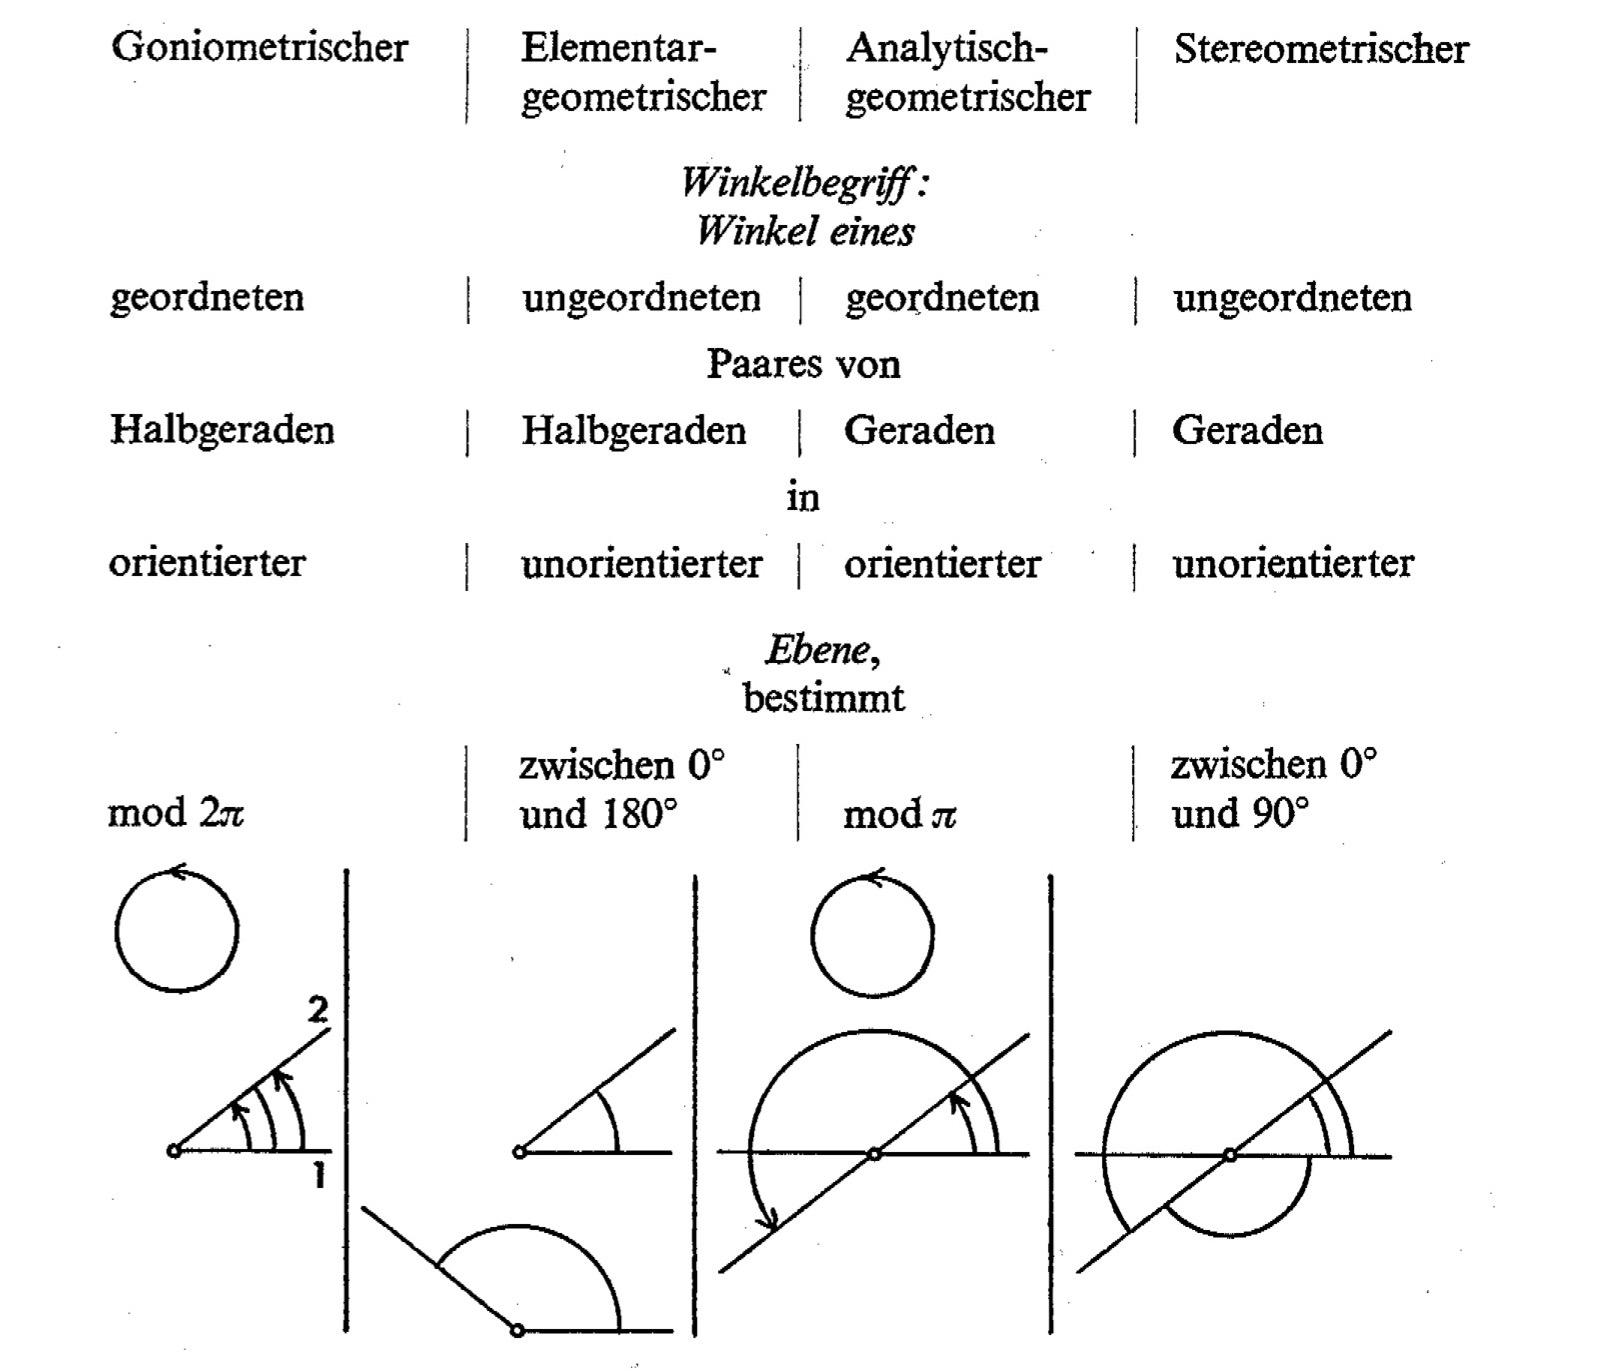
\includegraphics[width=0.75\linewidth]{pictures/1-FreudenthalWinkel} 

}

\caption{Winkelbegriffe nach Freudenthal (\citeproc{ref-Freudenthal:1973}{1973b, S. 441})}\label{fig:FreudenthalWinkel}
\end{figure}

Er diskutiert, welchen Einfluss die jeweilige Sichtweise auf dem Maßbereich hat, wie Winkel überhaupt gemessen werden können und wie mit Winkeln operiert werden kann. Was passiert denn, wenn man ein geordnetes Strahlenpaar in der orientierten Ebene spiegelt (vgl. \citeproc{ref-Freudenthal:1973}{Freudenthal, 1973b, 443~ff.})?

Wenn die Reihenfolge der Strahlen erhalten bleibt und die Winkelmessung aufgrund der Orientierung der Ebene vorgegeben ist, ändert sich damit ggf. auch das Maß des Winkels (siehe Abbildung \ref{fig:FreudenthalWinkelSpiegeln}).



\begin{figure}

{\centering 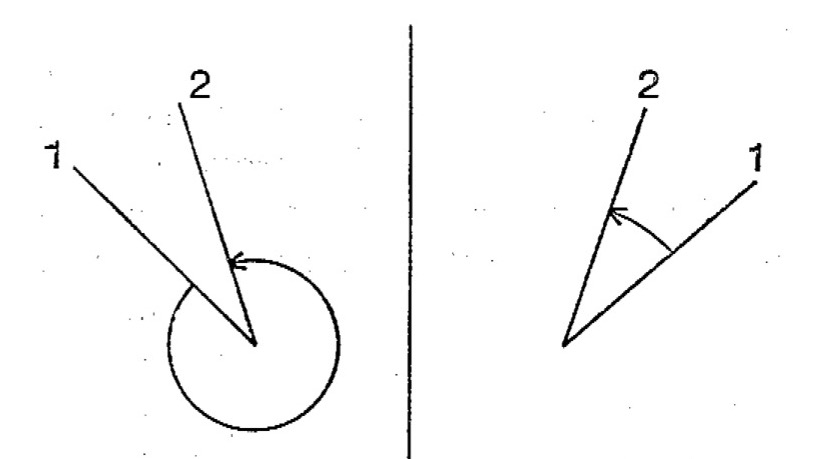
\includegraphics[width=0.5\linewidth]{pictures/1-FreudenthalWinkelSpiegeln} 

}

\caption{Spiegelung eines goniometrischen Winkels (\citeproc{ref-Freudenthal:1973}{Freudenthal, 1973b, 443})}\label{fig:FreudenthalWinkelSpiegeln}
\end{figure}

Hierzu stellt Freudenthal (\citeproc{ref-Freudenthal:1973}{1973b, 443~ff.}) weitere fachmathematische Ausführungen dar und schließt damit, dass der elementargeometrische, goniometrische und analytische Winkelbegriff aus fachlicher Sicht für den schulischen Lernpfad unentbehrlich sind (\citeproc{ref-Freudenthal:1973}{Freudenthal, 1973b, S. 449}).

Die \emph{Spezifizierung} besteht also darin, den Begriff zu schärfen und Operationen mit ihm zu beschreiben. Die \emph{Strukturierung} besteht u.~a. in der vernetzenden Analyse der verschiedenen Winkelbegriffe und der Schlussfolgerung ihrer gleichermaßen Bedeutsamkeit für den Schulunterricht.\index{Vier-Ebenen-Ansatz!formale Ebene|)}

\subsection{Semantische Ebene}\label{semantische-ebene}

Dazu,\index{Vier-Ebenen-Ansatz!semantische Ebene|(} welche Vorstellungen Schülerinnen und Schüler zum Winkelbegriff entwickeln sollen, sei u.~a. auf Krainer (\citeproc{ref-Krainer:1989}{1989}) und Mitchelmore \& White (\citeproc{ref-Mitchelmore:1998}{1998}) verwiesen. Eine grundsätzliche Schwierigkeit beim Unterrichten von Winkeln sind diverse und (scheinbar) nicht in Verbindung zu bringende Anwendungskontexte, die dennoch über denselben mathematischen Begriff beschrieben werden können. So ist das Sichtfeld eines Tieres ebenso wie die Umdrehung eines Wasserzählers über Winkel beschreibbar -- haben doch beide Situationen zunächst nichts miteinander zu tun.

Aufbauend auf den Arbeiten von Krainer (\citeproc{ref-Krainer:1989}{1989}) und Mitchelmore \& White (\citeproc{ref-Mitchelmore:1998}{1998}) können über eine Verknüpfung zur formalen Ebene mithilfe einer \emph{informationstheoretischen Winkeldefinition} (\citeproc{ref-Etzold2021}{Etzold, 2021, 39~f..}) vier Grundvorstellungen zum Winkelbegriff ausgearbeitet bzw. validiert werden:

\begin{itemize}
\tightlist
\item
  Winkel als Knick
\item
  Winkel als Feld
\item
  Winkel als Richtungsänderung
\item
  Winkel als Umdrehung
\end{itemize}

Dabei erhalten die \emph{Bestandteile} eines Winkels (Scheitelpunkt, Schenkel, ggf. Bereich zwischen den Schenkeln, Abweichungsmaß) eine besondere Bedeutung, über die sich auch eine sinnvolle Reihenfolge der Behandlung dieser Grundvorstellungen ableiten lässt. So »bietet es sich an, mit den Winkelfeldern zu beginnen. Bei diesen werden die meisten Bestandteile sichtbar (Scheitelpunkt, beide Schenkel als Begrenzungen sowie der zwischen den Schenkeln relevante Bereich) {[}\ldots{]}. Anschließend können Knicke oder Richtungsänderungen behandelt werden, woraufhin die Umdrehungen folgen.« (\citeproc{ref-Etzold2021}{Etzold, 2021, S. 60})

Die \emph{Spezifizierung} in diesem semantischen Teil ist demnach die Ausarbeitung der Grundvorstellungen. Die Begründung einer möglichen Reihenfolge kann der \emph{Strukturierung} des Lerngegenstands zugeordnet werden.\index{Vier-Ebenen-Ansatz!semantische Ebene|)}

\subsection{Konkrete Ebene}\label{konkrete-ebene}

Um\index{Vier-Ebenen-Ansatz!konkrete Ebene|(} die einzelnen Vorstellungen zu Winkeln aufzubauen, bedarf es charakteristischer Situationen, an denen der mathematische Kern der jeweiligen Vorstellung besonders gut sichtbar wird. Abbildung \ref{fig:Winkelsituationen} zeigt derartige \emph{Winkelsituationen} und die zugehörigen Grundvorstellungen (hier \emph{Winkelkontexte}).



\begin{figure}

{\centering 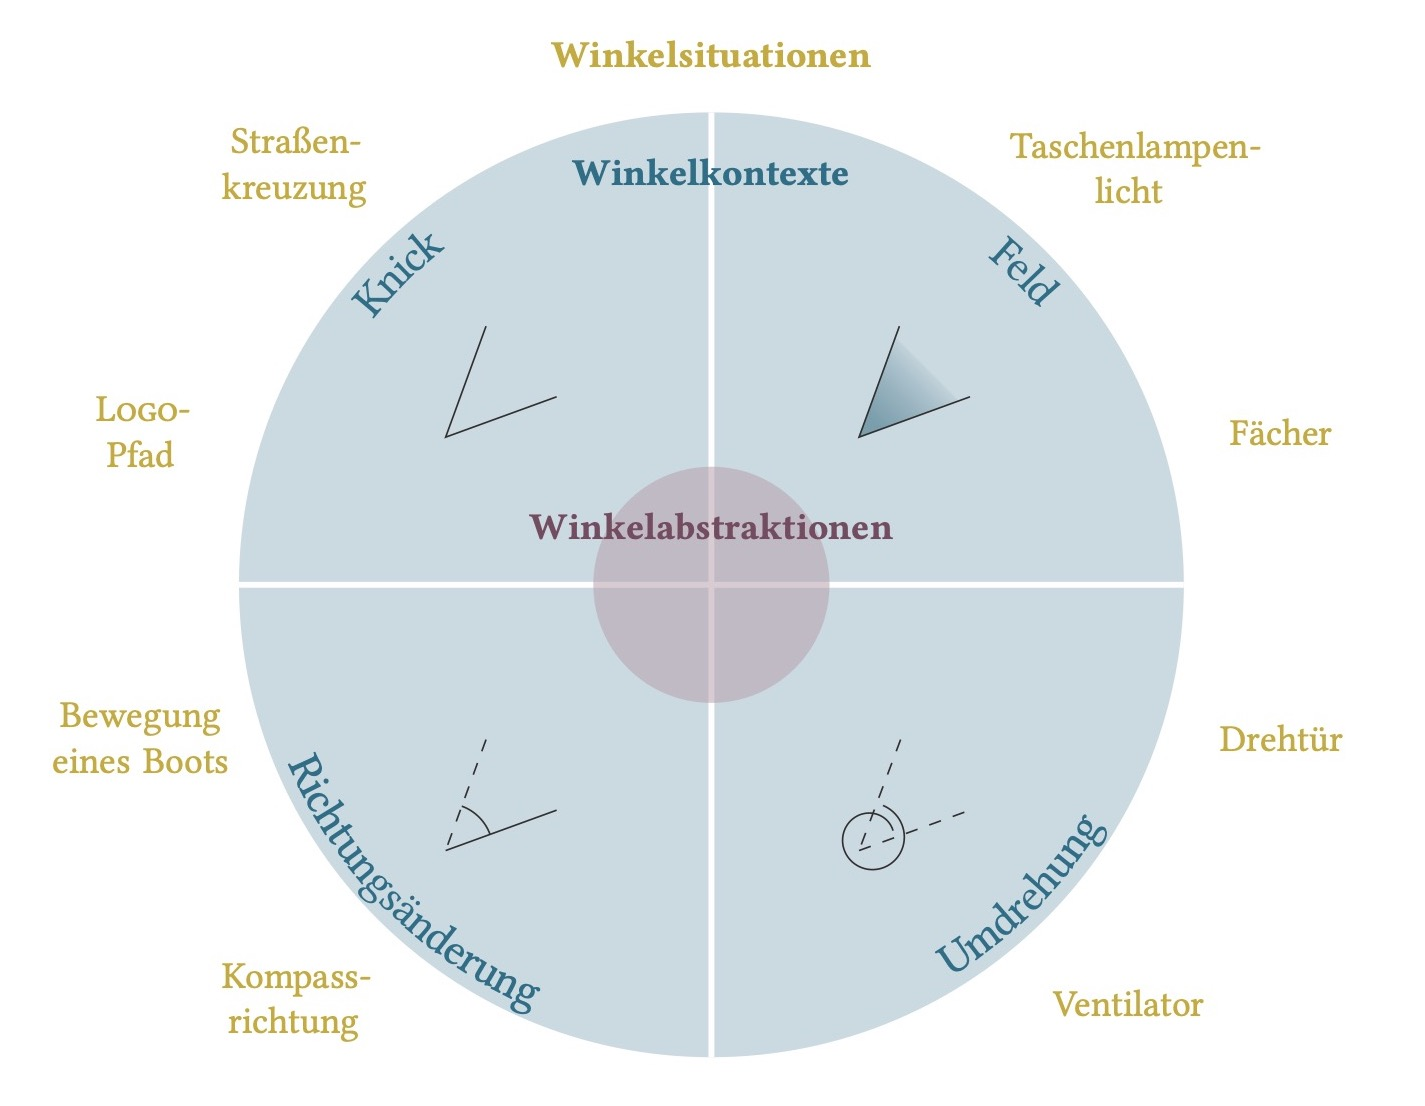
\includegraphics[width=0.75\linewidth]{pictures/1-Winkelsituationen} 

}

\caption{Winkelsituationen und -kontexte (\citeproc{ref-Etzold2021}{Etzold, 2021, S. 70})}\label{fig:Winkelsituationen}
\end{figure}

Exemplarisch für die Grundvorstellung des Winkels als Feld wird darauf aufbauend eine Lernumgebung und darin eingebettetes Unterrichtsmaterial entwickelt, mithilfe dessen die Grundvorstellung ausgebildet werden kann. An der konkreten Situation der \emph{Sichtfelder von Tieren} sollen die Schülerinnen und Schüler Handlungen ausführen, die es ihnen ermöglicht, den mathematischen Kern hinter dem konkreten Beispiel zu erkunden.

Die Schülerinnen und Schüler nutzen dazu eine App (siehe Abbildung \ref{fig:WinkelfarmApp}), in der mehrere Tiere mit ihren Sichtfeldern dargestellt werden können, und erhalten u.~a. folgende Aufgaben (vgl. \citeproc{ref-Etzold:2019Praxis4}{Etzold, 2019b, S. 8~ff.}):

\begin{enumerate}
\def\labelenumi{\arabic{enumi}.}
\tightlist
\item
  Setze das Schaf an eine Stelle, an der es von der Kuh gesehen wird, aber die Kuh selbst nicht sieht.
\item
  Setze das Schaf an eine Stelle, an der es nicht von der Kuh gesehen wird.
\item
  Das Schaf will die Kuh verwirren. Bewege es an möglichst viele Orte, an denen es von der Kuh gesehen wird.
\item
  Setze das Schaf an eine Stelle, an der es noch gerade so von der Kuh gesehen wird.
\item
  Wo muss das Schaf lang laufen, damit es die gesamte Zeit gerade so von der Kuh gesehen wird?
\end{enumerate}

An Aufgabe 5 kann z.~B. erkundet werde, dass sich das Schaf geradlinig auf der Grenze zwischen Sichtfeld und Nicht-Sichtfeld bewegen muss. In die eine Richtung ist die Bewegung beliebig fortsetzbar, in die andere durch den Kopf der Kuh begrenzt. Eine mathematische Verallgemeinerung dieser Handlung besteht dann in der Identifizierung des Schenkels (Begrenzung) als Strahl (nur in eine Richtung fortsetzbar) mit dem Scheitelpunkt (Kopf der Kuh) als \emph{Quelle} des Winkelfeldes.



\begin{figure}

{\centering 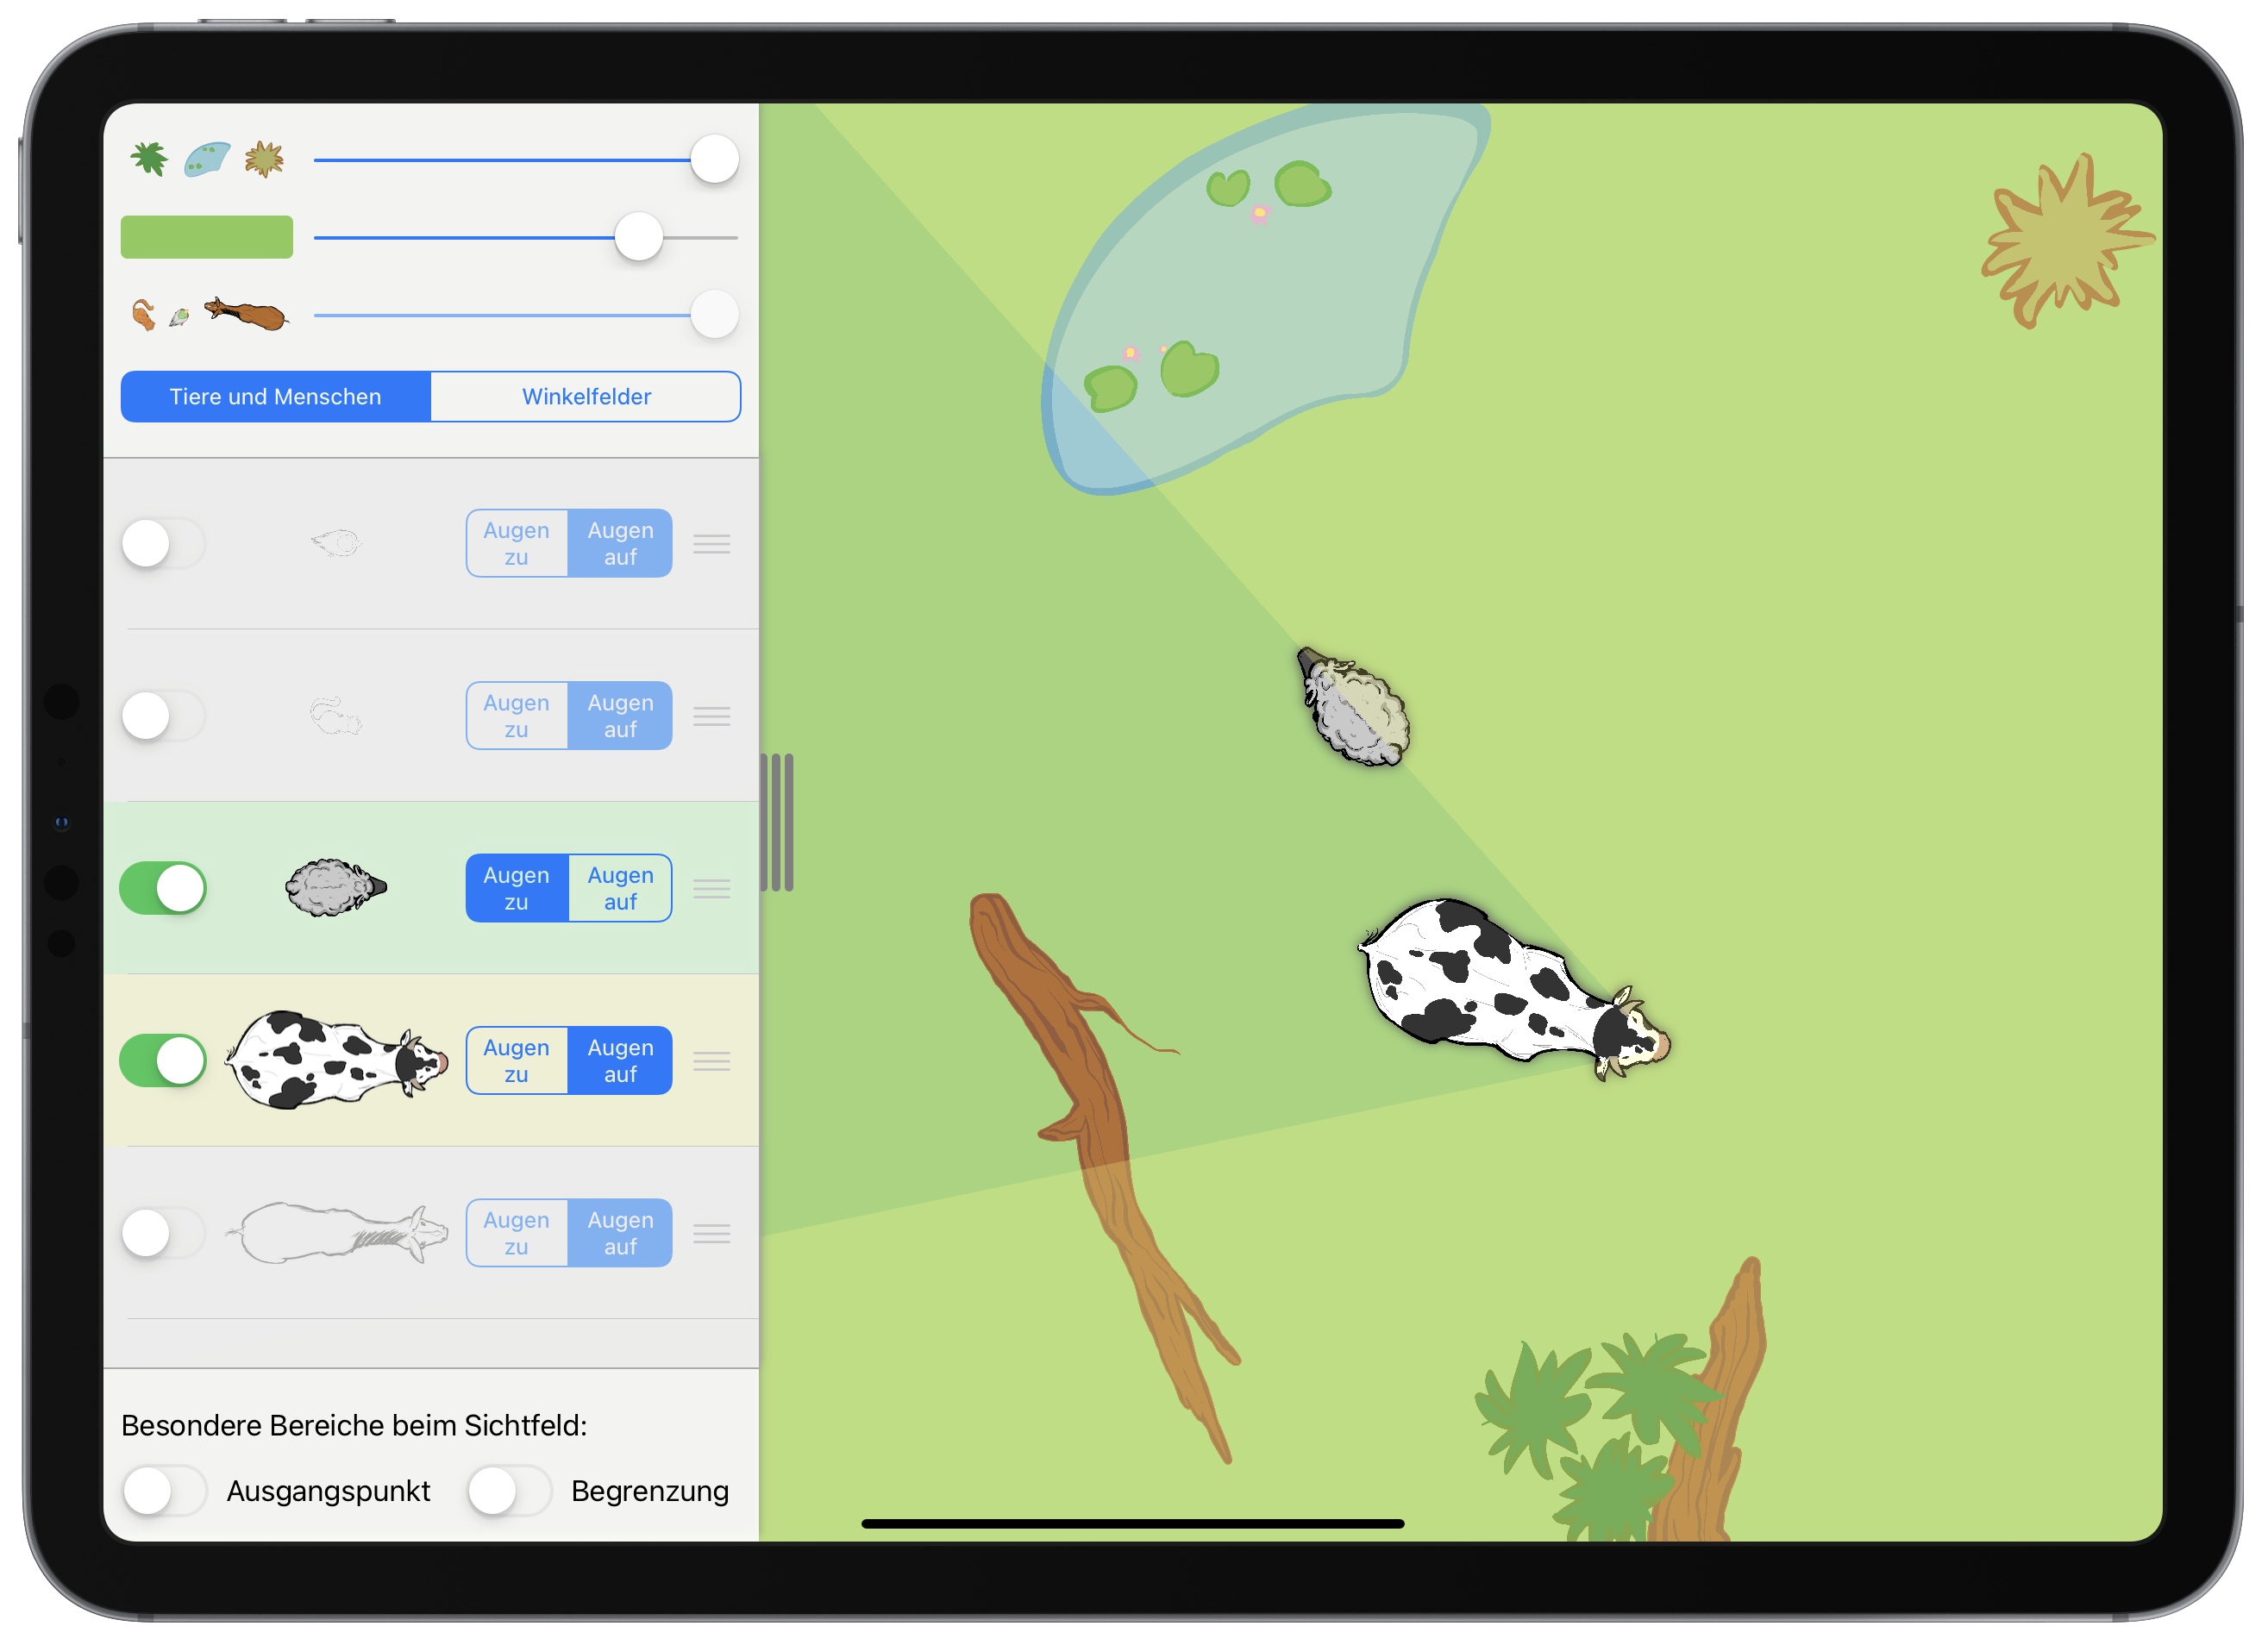
\includegraphics[width=0.75\linewidth]{pictures/1-Winkelfarm} 

}

\caption{Screenshot der App Winkel-Farm (\citeproc{ref-Etzold:2019}{Etzold, 2019a})}\label{fig:WinkelfarmApp}
\end{figure}

Als \emph{Spezifizierung} kann das Finden der Sichtfeld-Situation als charakterisches Beispiel für ein Winkelfeld angesehen werden. Die \emph{Strukturierung} führt zum dargestellten Lernpfad und den konkreten Aufgabenstellung, über die konkrete Handlungen verallgemeinert werden und damit das mathematische Verständnis aufgebaut wird.\index{Vier-Ebenen-Ansatz!konkrete Ebene|(}

\subsection{Empirische Ebene}\label{empirische-ebene}

Die\index{Vier-Ebenen-Ansatz!empirische Ebene|(} zuvor beschriebene Lernumgebung wurde in mehreren Zyklen erprobt und dabei die Qualität der Handlungen der Schülerinnen und Schüler beobachtet. Ein Ziel bestand darin, dass möglichst verallgemeinerbare Handlungen (wie oben am Beispiel des Schenkels beschrieben) durchgeführt werden.

Es wird erwartet, dass die Repräsentation eines Sichtfeldes von der Draufsicht über eine semintransparent ausgemalte Teilfläche der Ebene noch nicht bekannt ist. Um diese nachzuvollziehen und mit eigenen Erfahrungen in Bezug zu bringen, wird an den Beginn der Unterrichtsstunde ein Bild des Klassenraumes in der Draufsicht präsentiert (siehe Abbildung \ref{fig:Klassenraum}). Dann soll eine Schülerin oder ein Schüler beschreiben, was sie/er alles sieht, ohne den Kopf zu drehen. Dieser Bereich wird auf dem Bild eingezeichnet, so dass die Repräsentation des Sichtfeldes im Folgenden zur Verfügung steht.

\begin{figure}

{\centering 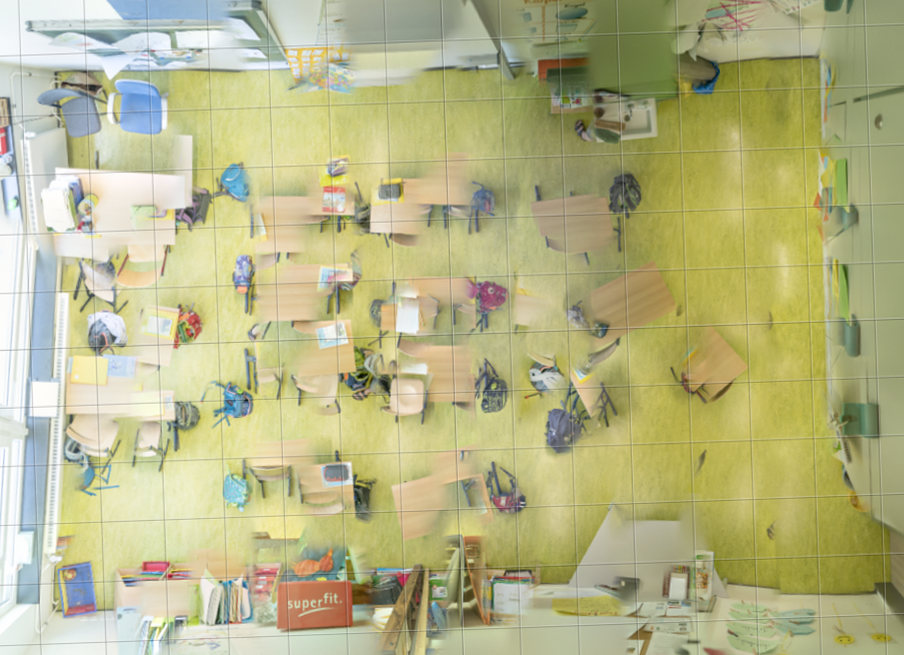
\includegraphics[width=0.75\linewidth]{pictures/1-Klassenraum} 

}

\caption{Klassenraum von oben (Foto: Christian Dohrmann)}\label{fig:Klassenraum}
\end{figure}

In der Erprobung konnte beobachtet werden, dass einige Bedienschwierigkeiten mit der Anwendung den Lernfortschritt hemmten. Dies konnte u.~a. dadurch verbessert werden, dass vor die eigentliche Erarbeitung eine freie Erkundungsphase mit der App (siehe Abbildung \ref{fig:WinkelfarmStart}) gesetzt wurde (\citeproc{ref-Etzold2021}{Etzold, 2021, S. 147, 152}). Durch spezifische Aufgabenstellungen wurden bestimmte Funktionen der App fokussiert:

\begin{figure}

{\centering 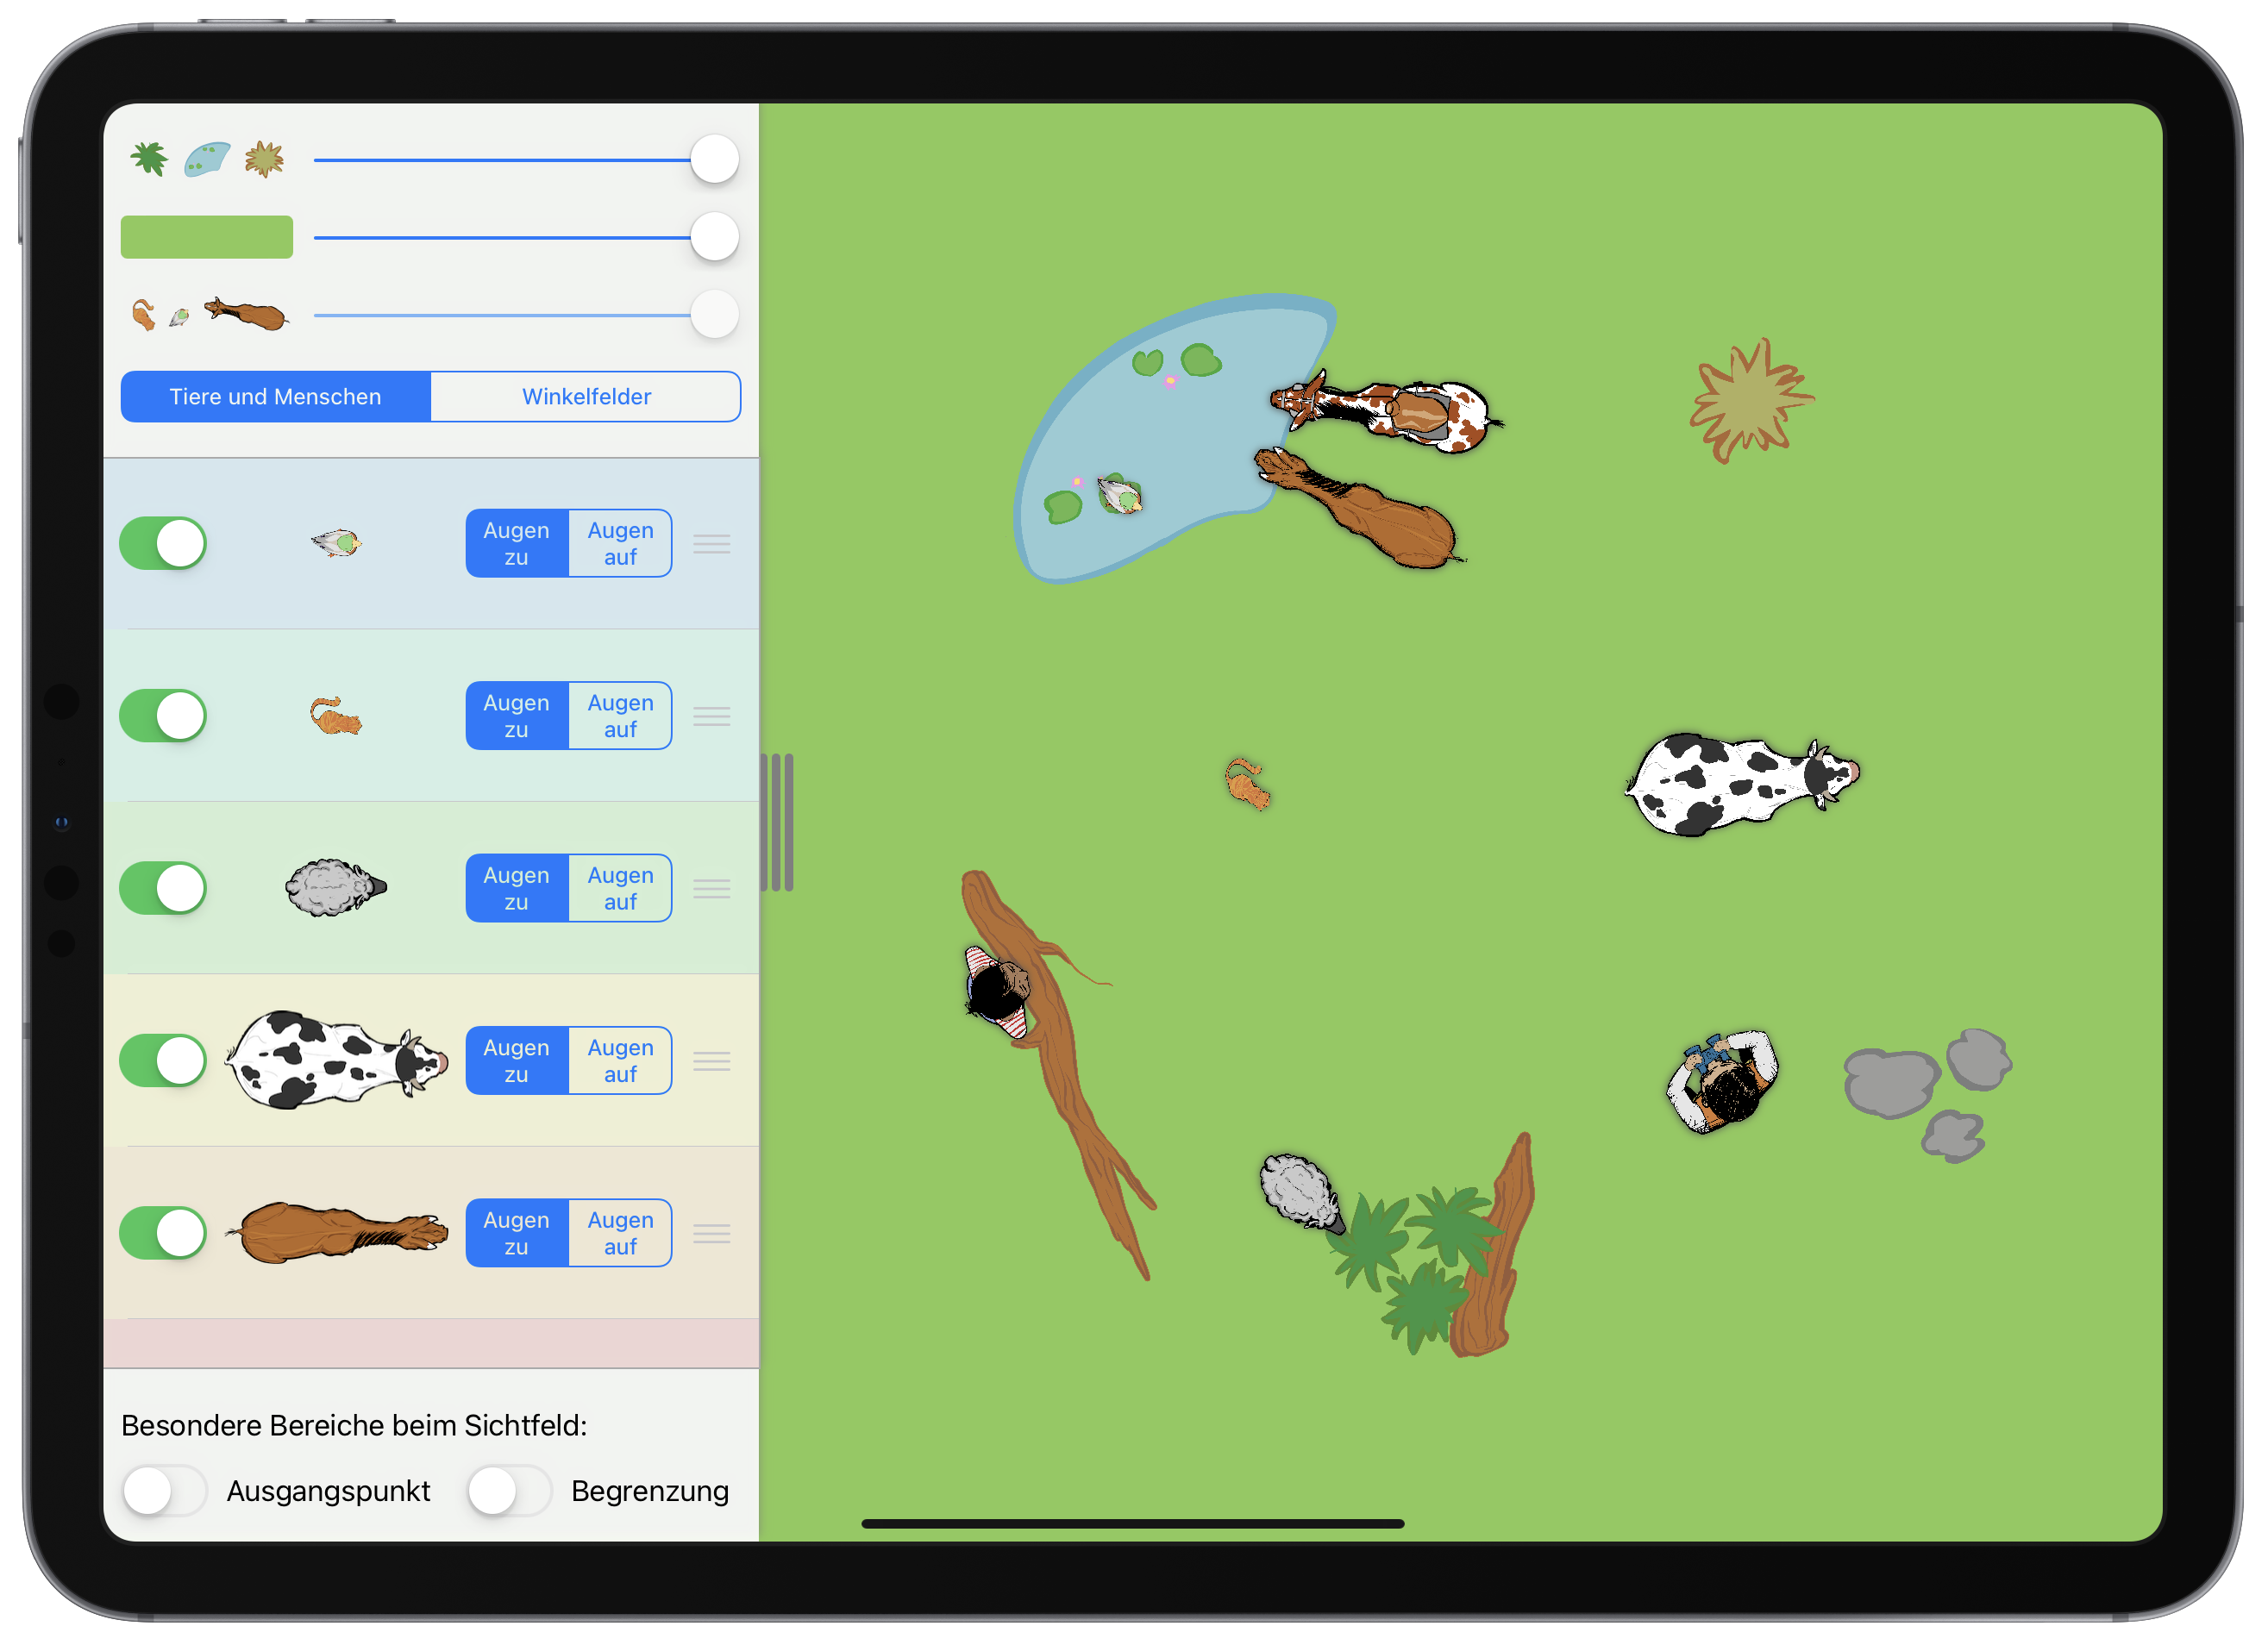
\includegraphics[width=0.75\linewidth]{pictures/1-WinkelfarmStart} 

}

\caption{Möglicher Startbildschirm für die freie Erkundungphase}\label{fig:WinkelfarmStart}
\end{figure}

\emph{»Das Pferd soll auf dem Steinpflaster stehen, die Frau soll auf dem Pferd sitzen/stehen. Das Pferd guckt in Richtung der grünen Büsche, die Frau hat die Augen zu. Gleichzeitig versteckt sich die Katze unter der Kuh.«}

Die Einführungsphase über das Klassenraumfoto folgt aus der \emph{Spezifizierung} innerhalb der empirischen Ebene. Das Hinzufügen der freien Erkundungsphase ist dagegen der \emph{Strukturierung} der Analyse zuzuordnen.\index{Winkel|)}\index{Vier-Ebenen-Ansatz!empirische Ebene|)}

\subsection{Verknüpfung der Ebenen}\label{verknuxfcpfung-der-ebenen}

An den Ausführungen ist schon sichtbar geworden, dass sich die Ebenen nicht immer trennen lassen und teilweise gegenseitig beeinflussen. Auch gehen oft Spezifizierung und Strukturierung ineinander über.

Das ist aber gar nicht schlimm, ganz im Gegenteil. Es zeigt wieder einmal, wie wichtig solch ein ganzheitlicher Ansatz ist, so dass eine stoffdidaktische Analyse aus den diversen Sichtpunkten heraus betrachtet werden sollte.

Wichtig ist v.~a., dass Sie sich als Lehrkraft stets darüber im Klaren sind, dass für eine stoffdidaktische Analyse verschiedene Perspektiven verfolgt werden müssen. Sehen Sie den Vier-Ebenen-Ansatz daher auch als Kontrollinstrument, ob Sie an alles gedacht haben, wenn Sie einen Lerngegenstand intensiv analysieren.

\section{Zum Nachbereiten}\label{vier-ebenen-nachbereitung}

\begin{enumerate}
\def\labelenumi{\arabic{enumi}.}
\tightlist
\item
  Lesen Sie den Artikel von Hußmann \& Prediger (\citeproc{ref-Hussmann:2016}{2016}) zum Vier-Ebenen-Ansatz.
\item
  Reflektieren Sie Ihre bisherige Fach- und Fachdidaktikausbildung in Mathematik dahingehend, welche der aufgeworfenen Fragen Sie zu konkreten Themenbereichen (nicht) beantworten könnten.
\end{enumerate}

\chapter{(Hoch-)Schulmathematik strukturieren}\label{hoch-schulmathematik-strukturieren}

\begin{quote}
\textbf{Ziele}

\begin{itemize}
\tightlist
\item
  Sie erkennen den Nutzen der Hochschulmathematik bei der Entscheidungsfindung zur Spezifizierung und Strukturierung der Schulmathematik auf der formalen Ebene des Vier-Ebenen-Ansatzes.
\item
  Sie kennen geeignete Quellen zur Beantwortung der Fragen auf der formalen Ebene des Vier-Ebenen-Ansatz\\
\item
  Sie kennen verschiedene Möglichkeiten, Mathematik zu strukturieren.\\
\item
  Sie können beschreiben, woher die verschiedenen Strukturierungsmöglichkeiten kommen.
\end{itemize}

\textbf{Material}

\begin{itemize}
\tightlist
\item
  Folien zum Kapitel 2 (\href{files/Stoffdidaktik2024-02-HochSchulmathematikStrukturieren.pdf}{pdf}, \href{files/Stoffdidaktik2024-02-HochSchulmathematikStrukturieren.key}{Keynote})
\end{itemize}
\end{quote}

\section{Doppelte Diskontinuität}\label{doppelte-diskontinuituxe4t}

Auf der \textcolor{formalColor}{formalen Ebene} des Vier-Ebenene-Ansatzes soll der zu betrachtende Lerngegenstand fachmathematisch untersucht werden, um eine erste Auswahl (\emph{Spezifizierung}) und Anordnung (\emph{Strukturierung}) der Lerninhalte zu ermöglichen. Dies ruft natürlich -- auch für Lerngegenstände der Grundschulmathematik -- danach, die im Studium erworbenen hochschulmathematischen Erkenntnisse zu nutzen. Dieser Ruf wird jedoch (scheinbar!) geschmälert durch eine offensichtliche Ungleichheit zwischen Schulmathematik und Hochschulmathematik. Felix Klein beschreibt dieses Phänomen, das sich insbesondere auf die Ausbildung von Lehrkräften auswirkt, bereits im Übergang vom 19. zum 20. Jahrhunderts als \textbf{\emph{doppelte Diskontinuität}}: »Der junge Student sieht sich am Beginn seines Studiums vor Probleme gestellt, die ihn in keinem Punkte mehr an die Dinge erinnern, mit denen er sich auf der Schule beschäftigt hat; natürlich vergißt er daher alle diese Sachen rasch und gründlich. Tritt er aber nach Absolvierung des Studiums ins Lehramt über, so soll er plötzlich eben diese herkömmliche Elementarmathematik schulmäßig unterrichten; da er diese Aufgabe kaum selbständig mit seiner Hochschulmathematik in Zusammenhang bringen kann, so wird er in den meisten Fällen recht bald die althergebrachte Unterrichtstradition aufnehmen, und das Hochschulstudium bleibt ihm nur eine mehr oder minder angenehme Erinnerung, die auf seinen Unterricht keinen Einfluß hat.« (\citeproc{ref-Klein1967}{Klein, 1967, S. 1})\footnote{Es handelt sich hier um den Nachdruck eines Werke, dessen erste Auflage 1908 erschien.}

Einen Ausweg, dieser doppelten Diskontinität zu entgehen, sah Klein in einer \textbf{\emph{Elementarmathematik vom höheren Standpunkte aus}} (\citeproc{ref-Klein1925}{Klein, 1925}, \citeproc{ref-Klein1955}{1955}, \citeproc{ref-Klein1967}{1967}). Dabei verfolgt er »das Ziel, im Anschluss an umfassende hochschulmathematische Erfahrungen die Schulmathematik in den erworbenen Wissenskanon fachlich einzubetten« (\citeproc{ref-Danckwerts2013}{Danckwerts, 2013, S. 78}).

Diesen Gedanken fortsetzend kann man auch »gleich am Anfang des Studiums direkt und explizit an die schulmathematischen Vorerfahrungen an{[}knüpfen{]}, bleibt inhaltlich bei diesen und arbeitet einen höheren Standpunkt heraus, der auf die vertiefte Auseinandersetzung mit der Oberstufenmathematik zielt und prinzipiell mit den bis dahin erworbenen (elementar-)mathematischen Mitteln auskommt.« (\citeproc{ref-Danckwerts2013}{Danckwerts, 2013, S. 78}) Eine solche Entwicklung hat das Projekt \emph{Mathematik Neu Denken} verfolgt, das gut 100 Jahre nach Kleins Publikationen die Lehramtsausbildung im Fach Mathematik weiterentwickeln wollte (\citeproc{ref-Beutelspacher2012}{Beutelspacher et al., 2012}). Entwickelt wird daraus eine \textbf{\emph{Schulmathematik vom höheren Standpunkt}}, die auf eine fachliche und verstehensorientierte Durchdringung der Schulmathematik zielt, »ohne im vollen Umfang auf das Instrumentarium der kanonischen {[}\ldots{]} {[}Hochschulmathematik{]} zurückgreifen zu müssen« (\citeproc{ref-Danckwerts2013}{Danckwerts, 2013, S. 87}).

Im Rahmen der Stoffdidaktik-Veranstaltung sollen beide Ansätze aufgegriffen und an konkreten Beispielen versucht werden, die Fragen der \textcolor{formalColor}{formalen Ebene} zu beantworten. Als bedeutsames Bindeglied zwischen Schul- und Hochschulmathematik stellen sich dabei fundamentale Ideen heraus, die auch schon auf die \textcolor{semanticColor}{semantische Ebene} des Vier-Ebenen-Ansatzes zielen -- siehe dazu Abschnitt \ref{fundamentale-ideen}.

\section{Geeignete Quellen}\label{geeignete-quellen}

\begin{itemize}
\item
  Neben den Werken von Felix Klein zu Beginn des 20. Jahrhunderts (\citeproc{ref-Klein1925}{Klein, 1925}, \citeproc{ref-Klein1955}{1955}, \citeproc{ref-Klein1967}{1967}) und aktuellen Ansätzen zum Umgang mit der doppelten Diskontinuität in der Lehramtsausbildung (\citeproc{ref-Ableitinger2013}{Ableitinger et al., 2013}; \citeproc{ref-Beutelspacher2012}{Beutelspacher et al., 2012}) liefern die in den 1970er Jahren von Hans Freudenthal verfassten Werke zur \emph{Mathematik als pädagogische Aufgabe} (\citeproc{ref-Freudenthal1973a}{Freudenthal, 1973c}, \citeproc{ref-Freudenthal:1973}{1973b}; englischsprachig auch digital verfügbar über \citeproc{ref-Freudenthal1973c}{Freudenthal, 1973a}) Ansätze, Schul- und Hochschulmathematik miteinander in Bezug zu bringen.
\item
  Ebenfalls hilfreich sind größere Nachschlagewerke zur Mathematik, bspw. die \emph{Kleine Enzyklopädie Mathematik} (\citeproc{ref-Gellert1986}{Gellert et al., 1986}).
\item
  Nicht zu unterschätzen für die fachmathematische Auseinandersetzung sind auch fachdidaktische Quellen, insbesondere zur \textbf{Didaktik der Sachgebiete}. Als digital verfügbare Quellen seien zu erwähnen:

  \begin{itemize}
  \tightlist
  \item
    \emph{Didaktik der Algebra: nach der Vorlage von Hans-Joachim Vollrath} (\citeproc{ref-Weigand2022}{Weigand et al., 2022})
  \item
    \emph{Didaktik der Geometrie für die Sekundarstufe I} (\citeproc{ref-Weigand2018}{Weigand et al., 2018})
  \item
    \emph{Didaktik der Analysis. Aspekte und Grundvorstellungen zentraler Begriffe} (\citeproc{ref-Greefrath2016}{Greefrath et al., 2016})
  \item
    \emph{Didaktik der Stochastik in der Sekundarstufe I} (\citeproc{ref-Kruger2015}{Krüger et al., 2015})
  \item
    \emph{Didaktik der Analytischen Geometrie und Linearen Algebra: Algebraisch verstehen -- Geometrisch veranschaulichen und anwenden} (\citeproc{ref-Henn2015}{Henn \& Filler, 2015})
  \item
    \emph{Mathematikunterricht in der Sekundarstufe II. Band 1: Fachdidaktische Grundfragen, Didaktik der Analysis} (\citeproc{ref-Tietze:2000a}{Tietze et al., 2000a})
  \item
    \emph{Mathematikunterricht in der Sekundarstufe II. Band 2: Didaktik der Analytischen Geometrie und Linearen Algebra} (\citeproc{ref-Tietze:2000}{Tietze et al., 2000b})
  \item
    \emph{Mathematikunterricht in der Sekundarstufe II. Band 3: Didaktik der Stochastik} (\citeproc{ref-Tietze:2002}{Tietze et al., 2002})
  \end{itemize}
\item
  Ebenfalls hilfreich für die fachliche Spezifizierung und Strukturierung kann die Darstellung der Fachinhalte in \textbf{Schulbüchern} sein. Hier bietet sich eine vergleichende Analyse mehrerer Schulbücher, auch unterschiedlicher Bundesländer, an.
\item
  Nur gering geeignet für die Spezifizierung und Strukturierung sind die Bildungsstandstandards und Rahmenlehrpläne. Sie bieten -- entsprechend ihrer Funktion -- bereits eine Auswahl der zu unterrichtenden Inhalte und schränken damit die fachdidaktische Diskussion diesbezüglich ein.
\end{itemize}

\section{Strukturierungsmöglichkeiten}\label{strukturierungsmuxf6glichkeiten}

Mathematik kann auf verschiedene Weisen strukturiert werden. Manche Strukturierungsmöglichkeiten orientieren sich stärker an der Fachwissenschaft (z.~B. \emph{Sachgebiete}), andere an der Bedeutung der Fachinhalte für die mathematische Kultur an sich (z.~B. \emph{Fundamentale Ideen}). Im Folgenden werden vier Strukturierungsmöglichkeiten vorgestellt.

\subsection{Sachgebiete}\label{sachgebiete}

Für die Fachwissenschaft Mathematik haben sich historisch verschiedene Unterdisziplinen entwickelt, die als Sachgebiete der Mathematik bezeichnet werden können. Schulrelevante Gebiete sind hierbei:

\begin{itemize}
\tightlist
\item
  Arithemtik
\item
  Algebra
\item
  Geometrie
\item
  Analysis
\item
  Stochastik
\item
  Lineare Algebra / Analytische Geometrie
\end{itemize}

Auch heute bilden sich diese und weitere Sachgebiete (z.~B. Numerik) in den Strukturen von universitären Lehrveranstaltungen, Forschungsrichtungen und nicht zuletzt der Strukturierung einzelner Lehrpläne der Schulen ab.

Für eine Vertiefung mit der Didaktik der Sachgebiete eignen sich u.~a. die in Abschnitt \ref{geeignete-quellen} dargestellten Quellen. Weiterhin werden Sie im Masterstudium im Modul \emph{Ausgewählte Themen der Mathematikdidaktik}\footnote{siehe Modulbeschreibung zum Modul \href{https://puls.uni-potsdam.de/qisserver/rds?state=verpublish&status=init&vmfile=no&moduleCall=modulansicht&publishConfFile=modulverwaltung&publishSubDir=up/modulbearbeiter&&modul.modul_id=3186&menuid=&topitem=Modulbeschreibung&subitem=}{MAT-LS-D3 bei PULS}} die Möglichkeit haben, sich mit der Didaktik einzelner Sachgebiete näher auseinanderzusetzen.

\subsection{Leitideen}\label{leitideen}

Die Strukturierung mathematischer Inhalte in Leitideen ist seit Anfang der 2000er Jahre im deutschen Bildungswesen etabliert, als die KMK\footnote{Mehr zur Kultusministerkonferenz (KMK) und ihrer eigentlichen Bezeichnungen siehe Wikipedia (\citeproc{ref-dewiki:228417777}{2022b}).} \textbf{Bildungsstandards} für den Mittleren Schulabschluss (2004), den Primarbereich (2005) und später auch die Allgemeine Hochschulreife (2012) herausgebracht hat. Darauf aufbauend wurden in den meisten Bundesländern die Lehrpläne angepasst.
Zwischenzeitlich wurden die Bildungsstandards für den Primarbereich sowie den Ersten und Mittleren Schulabschluss überarbeitet, für die gymnasiale Oberstufe gelten während der gerade laufenden Überarbeitung noch die von 2012. (\citeproc{ref-KMK:2012}{Sekretariat der Ständigen Konferenz der Kultusminister der Länder in der Bundesrepublik Deutschland, 2012}, \citeproc{ref-SekretariatderStandigenKonferenzderKultusministerderLanderinderBundesrepublikDeutschland2022a}{2022b}, \citeproc{ref-SekretariatderStandigenKonferenzderKultusministerderLanderinderBundesrepublikDeutschland2022}{2022a}).
In Brandenburg spiegeln sich die Bildungsstandards in den \textbf{Rahmenlehrplänen} für die Jahrgangsstufen 1~--~10 und die Gymnasiale Oberstufe wider (\citeproc{ref-MinisteriumfurBildungJugendundSportdesLandesBrandenburg2022}{Ministerium für Bildung, Jugend und Sport des Landes Brandenburg, 2022b}, \citeproc{ref-MinisteriumfuerBildungJugendundSportdesLandesBrandenburg2023}{2023}).

Im Laufe der letzten 20 Jahre haben sich für die Leitideen teils verschiedene Bezeichnungen ergeben. In den aktuellen Bildungsstandards des Ersten und Mittleren Schulabschlusses (\citeproc{ref-SekretariatderStandigenKonferenzderKultusministerderLanderinderBundesrepublikDeutschland2022}{Sekretariat der Ständigen Konferenz der Kultusminister der Länder in der Bundesrepublik Deutschland, 2022a}) werden verwendet:

\begin{itemize}
\tightlist
\item
  Leitidee Zahl und Operation
\item
  Leitidee Größen und Messen
\item
  Leitidee Strukturen und funktionaler Zusammenhang
\item
  Leitidee Raum und Form
\item
  Leitidee Daten und Zufall
\end{itemize}

Die Leitidee Zahl und Operation beispielweise »umfasst sinntragende Vorstellungen und Darstellungen von Zahlen und Operationen sowie die Nutzung von Rechengesetzen und Kontrollverfahren. Dazu gehören die sachgerechte Nutzung von Prozent- und Zinsrechnung ebenso wie kombinatorische Überlegungen und Verfahren, denen Algorithmen zu Grunde liegen.« (\citeproc{ref-SekretariatderStandigenKonferenzderKultusministerderLanderinderBundesrepublikDeutschland2022}{Sekretariat der Ständigen Konferenz der Kultusminister der Länder in der Bundesrepublik Deutschland, 2022a, S. 15}). Weiterhin werden diese Kompetenzen an spezifischen Fachinhalten konkretisiert, etwa: »Die Schülerinnen und Schüler {[}\ldots{]} • untersuchen Zahlen nach ihren Faktoren, in einfachen Fällen ohne digitale Mathematikwerkzeuge, • stellen Zahlen der Situation angemessen dar, z.B. unter anderem in Zehnerpotenzschreibweise, • rechnen mit natürlichen, ganzen und rationalen Zahlen, die im täglichen Leben vorkommen, sowohl zur Kontrolle als auch im Kopf und erklären die Bedeutung der Rechenoperationen {[}\ldots{]}« (\citeproc{ref-SekretariatderStandigenKonferenzderKultusministerderLanderinderBundesrepublikDeutschland2022}{Sekretariat der Ständigen Konferenz der Kultusminister der Länder in der Bundesrepublik Deutschland, 2022a, S. 15})

Die Leitideen werden in den Bildungsstandards als \textbf{inhaltsbezogene Kompetenzen} beschrieben, die mit Abschluss des ersten bzw. mittleren Schulabschlusses zu erreichen sind. Es handelt sich dabei um \textbf{Regelstandards}, also Kompetenzen, die »Schülerinnen und Schüler im Durchschnitt in einem Fach erreichen sollen« (\citeproc{ref-SekretariatderStandigenKonferenzderKultusministerderLanderinderBundesrepublikDeutschland2022}{Sekretariat der Ständigen Konferenz der Kultusminister der Länder in der Bundesrepublik Deutschland, 2022a, S. 2}). Diese sind abzugrenzen gegenüber \textbf{Basiskompetenzen} als »mathematisch zentrale, instrumentell bedeutsame und geradezu grundlegende Konzepte und Verfahren, die für die mathematische Kompetenzentwicklung unverzichtbar sind« (vgl. \url{https://pikas-mi.dzlm.de/node/92}). Für Basiskompetenzen gibt es derzeit in Deutschland keine politischen Dokumente wie Rahmenlehrpläne oder Bildungsstandards.

\subsection{Arten mathematischen Wissens}\label{arten-mathematischen-wissens}

Eine weitere Strukturierung mathematischen Wissens kann darin bestehen, den Blick darauf zu lenken, wie dieses Wissen angeeignet wird. So können ähnliche Aneigungsprozesse Motivation bieten, das Wissen entsprechend zu strukturieren und dies dann für die Gestaltung von Lehr-Lern-Prozessen nutzbar zu machen. Etabliert hat sich hierfür eine Unterscheidung in drei Arten mathematischen Wissens (vgl. \citeproc{ref-Vollrath2012}{Vollrath \& Roth, 2012, S. 45}~f.):

\begin{itemize}
\item
  \textbf{Begriffe.} Diese bilden das Grundgerüst der Mathematik und belegen Objekte gleicher Eigenschaft mit einem gemeinsamen Bezeichner. Neben der Begriffsfestlegung, i.~d.~R. über eine Definition, ist der Einsatz geeignter Beispiele und Gegenbeispiele essentiell beim Aufbau eines Begriffsverständnisses.
\item
  \textbf{Zusammenhänge} Diese beschreiben Eigenschaften von Begriffen und ihre Beziehungen zueinander. Klassischerweise gehören hierzu mathematische Sätze inkl. ihrer Beweise, aber auch präformale Begründungen. Bei Vollrath \& Roth (\citeproc{ref-Vollrath2012}{2012, 45~f.}) wird statt von \emph{Zusammenhängen} von \emph{Sachverhalten} gesprochen, ältere Quellen beziehen sich auch nur auf \emph{Sätze}.
\item
  \textbf{Verfahren.} Diese bestimmen, wie bestimmte Aufgaben zu lösen sind, z. B. schriftliche Rechenverfahren, Lösungsverfahren von Gleichungen und Gleichungssystemen.
\end{itemize}

Einige Autoren zählen zu den Verfahren auch heuristische Strategien zum Problemlösen oder die Anwendung des Permanenzprinzips (vgl. \citeproc{ref-Steinhofel1988}{Steinhöfel et al., 1988, S. 23}). Vollrath \& Roth (\citeproc{ref-Vollrath2012}{2012, S. 46}~ff.) ergänzen dagegen die drei Wissensarten noch:

\begin{itemize}
\tightlist
\item
  \textbf{Metamathematisches Wissen.} Darunter ist zu verstehen, \emph{wie} Mathematik betrieben wird, also bspw. welche Möglichkeiten es gibt, ein mathematisches Problem zu lösen oder eine Sachsituation mathematisch zu modellieren.
\end{itemize}

In den nächsten Kapiteln wird näher darauf eingegangen, wie Lernprozesse bei der Ausbildung der jeweiligen Wissensarten gestaltet werden können.

\subsection{Fundamentale Ideen}\label{fundamentale-ideen}

\subsubsection{Begriffsklärung}\label{fundamentale-ideen-begriffsklaerung}

Die Entwicklung Fundamentaler Ideen beruft sich auf Bruners Annahme, dass »jedes Kind {[}\ldots{]} auf jeder Entwicklungsstufe jeder Lehrgegenstand in einer intellektuell ehrlichen Form erfolgreich gelehrt werden« kann (vgl. \citeproc{ref-Bruner:1976}{Bruner, 1976, S. 77}). Voraussetzung dafür ist, dass die \emph{Struktur} eines Inhaltsbereichs in einer Art und Weise präsentiert wird, dass sie dem Kind zugänglich wird. Diese \emph{hinter den Dingen} liegende Struktur hebt sich vom konkreten Inhaltsbereich ab, ist allgemeinerer Natur und kann daher über \emph{Fundamentale Ideen} beschrieben werden.

Ziel der Orientierung des Unterrichtens an Fundamentalen Ideen besteht v.~a. darin, die (oftmals) isolierten Stoffelemente einzuordnen und in einem größeren Ganzen zu sehen. Im Umkehrschluss heißt dies aber auch, dass die Auswahl des konkreten Stoffes daran orientiert sein muss, wie dieser dazu beitragen kann, den dahinter liegenden mathematischen Kern und die zugehörigen Fundamentalen Ideen zu vertreten.

Die dazu seit den 1960er Jahren in Gang gesetzte Forschung führte zu vielfältigen Vorschlägen Fundamentaler Ideen der Mathematik -- jedoch bisher nicht zu einem allgemeingültigen Katalog. Dieser Vielfalt in den Formulierungen und Kategorisierungen kann begegnet werden, indem Fundamentale Ideen über Eigenschaften charakterisiert werden. Schwill (\citeproc{ref-Schwill:1994}{1994}) schlägt hierzu vor.

»Eine \textbf{Fundamentale Idee}\index{Fundamentale Idee|textbf} bzgl. eines Gegenstandsbereichs (Wissenschaft, Teilgebiet) ist ein \textbf{Denk-, Handlungs-, Beschreibungs- oder Erklärungsschema}, das

\begin{enumerate}
\def\labelenumi{\arabic{enumi}.}
\tightlist
\item
  in verschiedenen Gebieten des Bereichs vielfältig anwendbar oder erkennbar ist (\textbf{Horizontalkriterium}),\index{Fundamentale Idee!Horizontalkriterium|textbf}
\item
  auf jedem intellektuellen Niveau aufgezeigt und vermittelt werden kann (\textbf{Vertikalkriterium}),\index{Fundamentale Idee!Vertikalkriterium|textbf}
\item
  in der historischen Entwicklung des Bereichs deutlich wahrnehmbar ist und längerfristig relevant bleibt (\textbf{Zeitkriterium}),\index{Fundamentale Idee!Zeitkriterium|textbf}
\item
  einen Bezug zu Sprache und Denken des Alltags und der Lebenswelt besitzt (\textbf{Sinnkriterium}).\index{Fundamentale Idee!Sinnkriterium|textbf}«
\end{enumerate}

Fundamentale Ideen haben zwar ihren Ursprung in der Fachstruktur, aber sie »sind nicht Elemente der Wissenschaft an sich, sondern Produkte unseres Verstandes, die wir der Wissenschaft aufprägen. Folglich können sie nur relativ zum Menschen objektiviert werden« (\citeproc{ref-Schubert:2011}{Schubert \& Schwill, 2011, S. 62}).

\begin{quote}
\textbf{Überblick zur historischen Entwicklung Fundamentaler Ideen}

\begin{itemize}
\tightlist
\item
  von der Bank (\citeproc{ref-Bank:2016}{2016, 37~ff.}): \emph{Fundamentale Ideen der Mathematik: Weiterentwicklung einer Theorie zu deren unterrichtspraktischer Nutzung}
\end{itemize}
\end{quote}

Für Ihre stoffdidaktische Analyse können Fundamentale Ideen insbesondere hilfreich für die \textbf{Dekonstruktion} des Fachwissens und anschließende \textbf{Rekonstruktion} des Schulwissens sein.

Wenn sie also beispielsweise eine stoffdidaktische Analyse zur Flächeninhaltsberechnung durchführen, setzen Sie sich mit der Fundamentalen Idee des \emph{Messens}\index{Messen} auseinander. Dabei verstehen Sie Messvorgänge als Vergleiche zu einem Standardmaß (z.~B. Kästchen auszählen), erkennen Zerlegungs- und Ergänzungsgleichheit als notwendige Prinzipien zur präziseren Beschreibung, sehen Dreiecke als bedeutsame Basisfiguren für Flächeninhaltsberechnungen an und haben den Blick für die Integralrechnung als verallgemeinerbare Methode zur Flächeninhaltsbestimmung krummliniger Figuren (vgl. \citeproc{ref-Vohns:2000}{Vohns, 2000, 98~ff.}). Sie \emph{dekonstruieren} (zerlegen) damit Ihr eigenes mathematisches Fachwissen.

Nun sind Sie in der Lage, das Wissen zur Flächeninhaltsberechnung für Schülerinnen und Schüler neu aufzubauen, also zu \emph{rekonstruieren} und (unter Hinzunahme der Betrachtung von Grundvorstellungen und den restlichen Ebenen des Vier-Ebenen-Ansatzes) einen Lernpfad zu entwickeln. Im Zusammenhang mit der Integralrechnung kann dies z.~B. heißen, dass Sie parallel zum Bilden von Ober- und Untersummen noch einmal eine krummlinig begrenzte Fläche durch Kästchen auszählen lassen -- ggf. mit unterschiedlicher Feinheit und einer Abschätzung nach oben und nach unten. Die Fundamentalen Ideen haben für Sie damit auch eine \emph{ordnende Funktion} des Unterrichtsstoffes.

\begin{figure}

{\centering 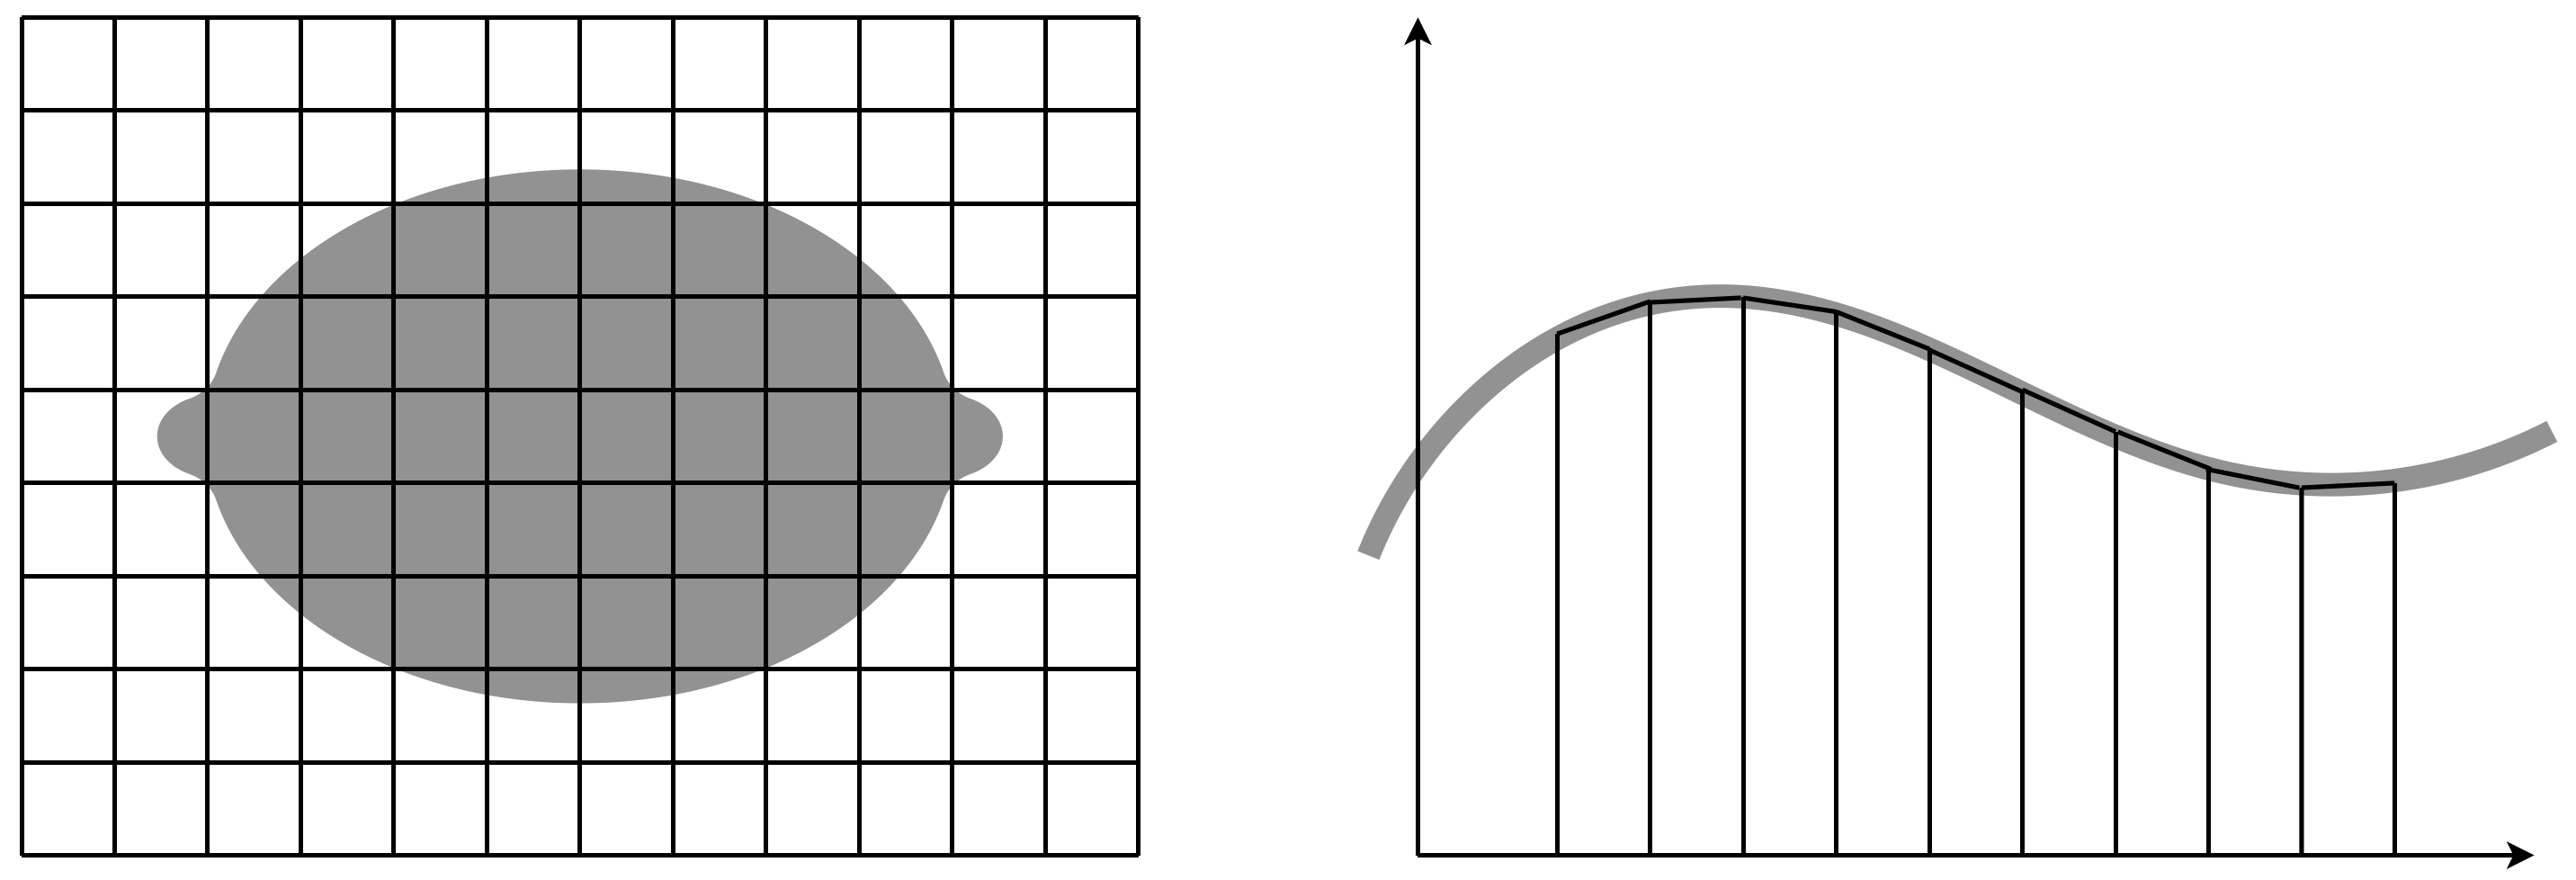
\includegraphics[width=0.75\linewidth]{pictures/3-Flaeche} 

}

\caption{Flächeninhaltsbestimmung}\label{fig:Flaeche}
\end{figure}

\subsubsection{Auswahl Fundamentaler Ideen}\label{auswahl-fundamentaler-ideen}

Das Fehlen eines allgemeingültigen Katalogs sollte nicht davon abhalten, bestehende Auflistungen und Strukturierungen Fundamentaler Ideen zu betrachten. von der Bank (\citeproc{ref-vonderBank:2013}{2013, S. 103}) und Lambert (\citeproc{ref-Lambert:2012}{2012}) diskutieren eine Kategorisierung Fundamentaler Ideen in drei Bereiche:

\begin{itemize}
\item
  \textbf{Inhaltsideen} beziehen sich auf konkrete Inhaltsbereiche der Mathematik, die die Kriterien Fundamentaler Ideen erfüllen können. Nicht ganz zufällig spiegeln diese sich in den Leitideen der Bildungsstandards wider (siehe Abschnitt \ref{leitideen}).
\item
  \textbf{Schnittstellenideen} haben die Eigenschaft, dass durch sie die »Mathe(matik) wirkt« und »auch für andere Fächer in ihrer je spezifischen Weise relevant sind« (\citeproc{ref-Lambert:2012}{Lambert, 2012}). Damit korrelieren sie mit den prozessbezogenen Kompetenzen der Bildungsstandards.
\item
  \textbf{Tätigkeitsideen} beziehen sich insbesondere auf innermathematische Tätigkeiten, die sich über verschiedene Inhaltsbereiche hinweg zeigen. Lambert (\citeproc{ref-Lambert:2012}{2012}) betont, dass es diese (über die Bildungsstandards hinaus) ebenfalls zu beachten gilt, wenn man einen reichhaltigen Mathematikunterricht bewirken möchte.
\end{itemize}

Beispiele derartiger Tätigkeitsideen sind:

\begin{itemize}
\tightlist
\item
  Approximierung
\item
  Optimierung
\item
  Linearität/Linearisierung
\item
  Symmetrie
\item
  Invarianz
\item
  Rekursion
\item
  Vernetzung
\item
  Ordnen
\item
  Strukturierung
\item
  Formalisierung
\item
  Exaktifizierung
\item
  Verallgemeinern
\item
  Idealisieren
\end{itemize}

Im Rahmen des Projektmoduls \emph{Erweitertes Fachwissen für den schulischen Kontext in Mathematik}\footnote{siehe Modulbeschreibung zum Modul \href{https://puls.uni-potsdam.de/qisserver/rds?state=verpublish&status=init&vmfile=no&moduleCall=modulansicht&publishConfFile=modulverwaltung&publishSubDir=up/modulbearbeiter&&modul.modul_id=3156&menuid=&topitem=Modulbeschreibung&subitem=}{MAT-LS-7 bei PULS}} werden Sie insbesondere Bezüge zwischen Schul- und Hochschulmathematik auf Basis Fundamentaler Ideen herstellen, wofür die Inhalts- und Tätigkeitsideen von hoher Relevanz sind.

\subsubsection{Beispiel Linearität}\label{beispiel-linearitaet}

\paragraph*{Horizontal- und Vertikalkriterium}\label{horizontal--und-vertikalkriterium}
\addcontentsline{toc}{paragraph}{Horizontal- und Vertikalkriterium}

Linearität\index{Linearität|(}\index{Fundamentale Idee!Horizontalkriterium|(}\index{Fundamentale Idee!Vertikalkriterium|(} ist ein wesentliches Konzept über die gesamte Schullaufbahn hinweg (und darüber hinaus). Dies spiegelt sich in vielfältigen Themenbereichen wider, die sowohl die Breite (\emph{Horizontalkriterium}) als auch Tiefe (\emph{Vertikalkriterium}) von Linearität und (später) auch Linearisierung zeigen. Dieser Abschnitt orientiert sich an den Darstellungen von Danckwerts (\citeproc{ref-Danckwerts:1988}{1988}).

\begin{itemize}
\tightlist
\item
  Linearität als Phänomen tritt schon im Geometrieunterricht der Grundschule mit \textbf{Geraden} als essentielle geometrische Objekte auf. In der euklidischen Geometrie sind Geraden neben Punkten die Basisobjekte eines axiomatischen Aufbaus.
\item
  Das \textbf{Distributivgesetz} \(a\cdot (b+c) = a\cdot b + a\cdot c\), das ebenfalls bereits in der Grundschule behandelt wird, beschreibt einen linearen Vorgang und bietet die Grundlage für die halbschriftliche Multiplikation. Über die Schulmathematik hinaus dient es z.~B. als eines der Vektorraumaxiome (Skalarmultiplikation).
\item
  Das Bestimmen eines \textbf{Rechteckflächeninhalts} ist ein linearer Vorgang: Ein Rechteck, das doppelt so breit ist, hat (bei gleicher Höhe) einen doppelt so großen Flächeninhalt. Betrachtet man diese Eigenschaft nicht als Phänomen, sondern als Forderung an eine Flächeninhaltsformel, so kann aus den Bedingungen \(A(a_1+a_2,b) = A(a_1,b) + A(a_2,b)\) und \(A(a,b_1+b_2) = A(a,b_1)+A(a,b_2)\) sowie der Stetigkeit in \(\mathbb{R}^+\) die Formel \(A(a,b) = a\cdot b\) abgeleitet werden.
\item
  Lineare Zuordnungen der Art \(f(x+y) = f(x)+f(y)\) werden zu Beginn der Sekundarstufe I als \textbf{proportionale Zuordnungen} behandelt. Dies wird fortgeführt bei \textbf{linearen Funktionen} der Art \(f(x) = mx+n\), in der Fachmathematik als affin-lineare Abbildungen bezeichnet.
\item
  \textbf{Lineare Gleichungen und Gleichungssysteme} sind ebenfalls bedeutsamer Bestandteil des Mathematikunterrichts. Überhaupt baut die gesamte \textbf{Lineare Algebra} auf lineare und affin-lineare Abbildungen auf.
\item
  Die \textbf{Strahlensätze} beschreiben ebenfalls ein lineares Verhalten: Geradenabschnitte in \(c\)-facher Entfernung sind \(c\) mal so lang.
\end{itemize}

\begin{figure}

{\centering 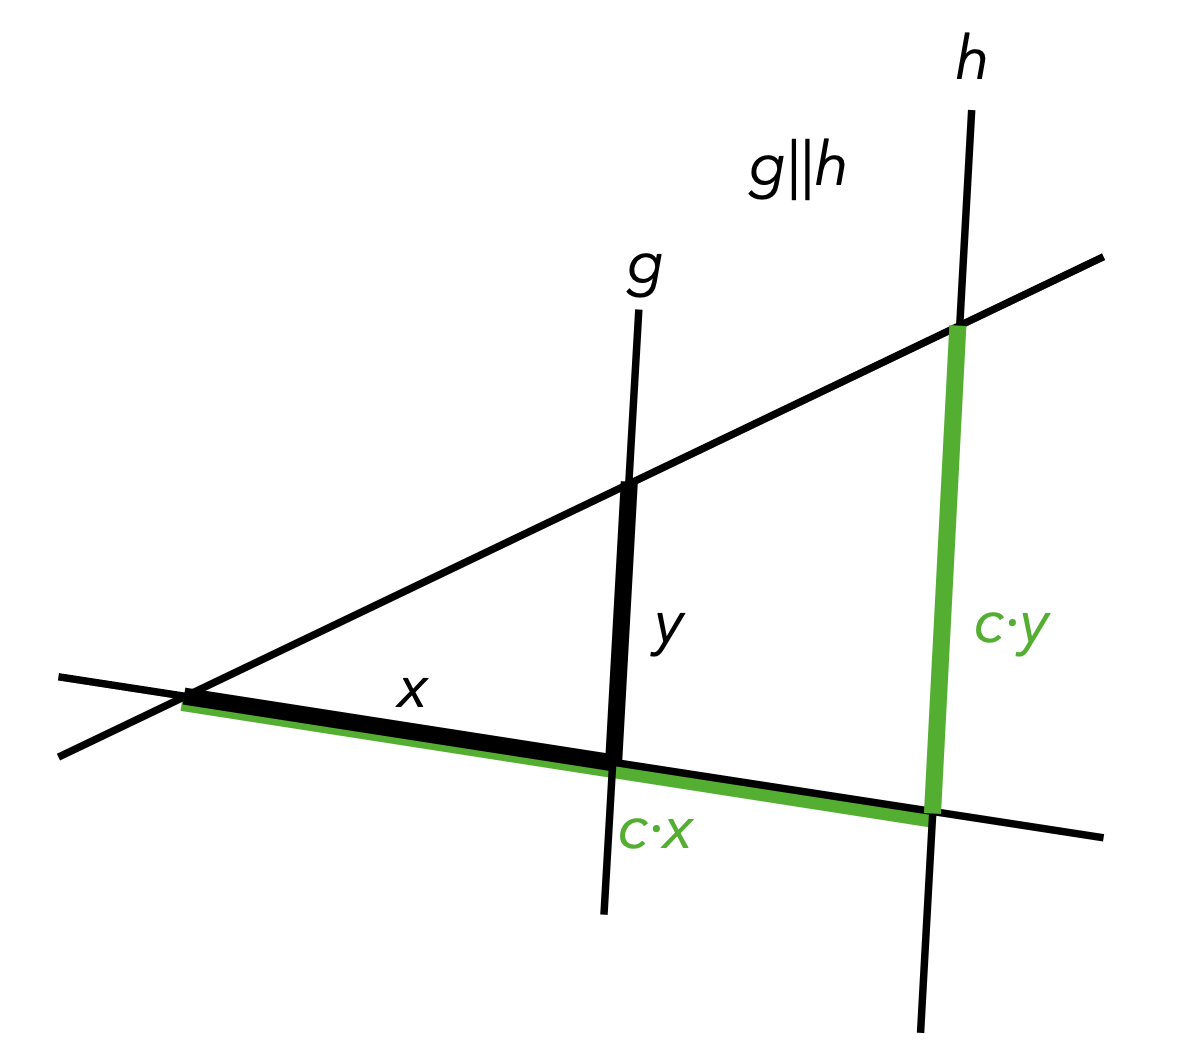
\includegraphics[width=0.5\linewidth]{pictures/3-Strahlensatz} 

}

\caption{Strahlensatzfigur}\label{fig:Strahlensatz}
\end{figure}

\begin{itemize}
\tightlist
\item
  Beim \textbf{Ableitungsbegriff} ist eine wesentliche Vorstellung, dass die Funktion in der Umgebung der zu betrachtenden Stelle linearisiert wird. Insbesondere bei höherdimensionalen Funktionen wird der Linearisierungsansatz weiterverfolgt. Die ebenfalls vorherrschende Tangentenvorstellung ist auf mehr als drei Dimensionen nicht mehr anschaulich übertragbar -- der Linearisierungsansatz weist hier aufgrund seiner algebraischen Beschreibung die bessere Verallgemeinerbarkeit auf.
\item
  Eng an den Linearisierungsansatz angelehnt ist die \textbf{lineare Approximation} von Funktionen (z.~B. \(\sin(x)\approx x\) für \(x\approx 0\)). Die führt sich in der Hochschulmathematik fort, beispielsweise bei Taylor-Reihen.
\item
  Das Bedürfnis der Linearisierung, insbesondere aus der Physik heraus, zeigt sich auch bei der Nutzung \textbf{spezifisch skalierter Diagrammachsen}, z.~B. von Logarithmuspapier. Wegen der Äquivalenz von \(y = c\cdot a^x\) und \(\ln y = (\ln a )\cdot x + \ln c\) lassen sich beliebige Exponentialfunktionen auf Logarithmuspapier als lineare Funktionen darstellen.
\item
  Verschiedene Näherungsverfahren, wie das \textbf{Newton-Verfahren}, bedienen sich ebenfalls der Linearisierung.
\end{itemize}

An dieser Stelle sei darauf hingewiesen, dass Linearität derart fundamental ist, dass selbst nicht-lineare Zusammenhänge häufig fälschlicherweise als linear angenommen werden. Dies zeigt sich zum Beispiel an den Fehlannahmen \((x+y)^2 \overset{?!}{=} x^2+y^2\), \(\sqrt{x+y} \overset{?!}{=} \sqrt{x}+\sqrt{y}\) oder \(\sin(x+y) \overset{?!}{=} \sin(x)+\sin(y)\). Derartige Fehler können Sie als Lehrkraft besser einordnen (und korrigieren), wenn Sie sich der Fundamentalen Idee \emph{Linearität} (die hier eben \emph{nicht} gilt) bewusst sind. Insbesondere spricht dies auch für ein Explizitmachen der Fundamentalen Idee Ihren Schülerinnen und Schülern gegenüber, so dass Sie derartigen Fehlern nicht nur mit Gegenbeispielen entgegen treten können, sondern auch eine strukturelle Einordnung sichtbar machen können.

Gerade wegen der genannten Fehlannahmen und der für die Schülerinnen und Schüler i.~d.~R. nicht in Zusammenhang gebrachten Dualität aus \emph{geradlinig} und \emph{additiv und homogen} sehen Tietze et al. (\citeproc{ref-Tietze:2002}{2002, S. 39}) die Linearität dagegen nicht als eine im Mathematikunterricht etablierte Fundamentale Idee, »die die Schüler erkennen und die ihr Denken ordnet und anregt«.\index{Fundamentale Idee!Horizontalkriterium|)}\index{Fundamentale Idee!Vertikalkriterium|)}

\paragraph*{Zeit- und Sinnkriterium}\label{zeit--und-sinnkriterium}
\addcontentsline{toc}{paragraph}{Zeit- und Sinnkriterium}

Linearität\index{Fundamentale Idee!Zeitkriterium|(}\index{Fundamentale Idee!Sinnkriterium|(} zeigt sich auch in der historischen Entwicklung der Mathematik als eine prägende Leitlinie, womit sie das \emph{Zeitkriterium} Fundamentaler Ideen erfüllt. In der Linearen Algebra sei beispielsweise das Lösen linearer Gleichungssysteme im 18. Jahrhundert bis hin zum Gauß-Algorithmus im 19. Jahrhundert oder die Darstellung linearer Vorgänge mit Matrizen im 17./18. Jahrhundert erwähnt (vgl. \citeproc{ref-Tietze:2000}{Tietze et al., 2000b, 73~ff.}). In der Analysis spiegelt sich die Linearität bzw. Linearisierung in der gesamten Differenzialrechnung wider, von der Interpolation nach der Jahrtausendwende über Taylors \emph{Linear perspective} von 1715 (vgl. \citeproc{ref-Bruckler:2018}{Brückler, 2018, 39,119}) bis in die Gegenwart der linearen Modellierung nichtlinearer Zusammenhänge.

\begin{quote}
\textbf{Historische Originalausgabe}

Taylor (\citeproc{ref-Taylor:1715}{1715}): \emph{Linear perspective}
\end{quote}

Auch Alltagssituationen bzw. die Alltagssprache ist von Linearität geprägt. Beispielsweise treten proportionale Zuordnungen unmittelbar beim Einkaufen auf, wenn Waren abgewogen und der Preis bestimmt wird. Auch reale Messvorgänge, wie z.~B. die Geschwindigkeitsmessung, beziehen sich in der Regel auf die Messung von (sehr kurzen) Zeitintervallen, in denen ein lineares Verhalten angenommen wird. Das \emph{Sinnkriterium} zeigt sich aber auch in Begriffen wie \emph{lineares Fernsehen} oder \emph{lineare Erzählungen}. Dies ist zwar keine mathematische Linearität im Sinne der Formel \(f(x+y) = f(x) +f(y)\), aber der Begriff findet in einer verwandten Bedeutung in der Alltagssprache Verwendung.\index{Linearität|)}\index{Fundamentale Idee!Zeitkriterium|)}\index{Fundamentale Idee!Sinnkriterium|)}

\subsubsection{Gegenbeispiele}\label{gegenbeispiele}

Zur Verständnisförderung sollen noch ein paar Gegenbeispiele für Fundamentale Ideen angebracht werden.

\begin{itemize}
\tightlist
\item
  Das bereits erwähnte \textbf{Distributivgesetz} an sich ist zwar elementar, aber ihm fehlt die Weite, womit es nicht das Horizontalkriterium erfüllt. Die \emph{Linearität} als dahinterliegende Idee ist dagegen weit genug (vgl. ähnliche Argumentation zum \textbf{Kommutativgesetz} und der dahinterliegenden Idee der \emph{Invarianz} bei \citeproc{ref-Schubert:2011}{Schubert \& Schwill, 2011, S. 63}).
\item
  Der \textbf{Umkehrfunktion} fehlt das Sinnkriterium, da dieser Begriff in der Lebenswelt außerhab der Mathematik kaum von Relevanz ist. Dahinter liegt vielmehr die Idee der \emph{Reversibilität} als »Umkehrbarkeit von Operationen mit Wiederherstellung des Ausgangszustandes« (\citeproc{ref-Schubert:2011}{Schubert \& Schwill, 2011, S. 63}).
\end{itemize}

\section{Beispiel Negative Zahlen}\label{beispiel-negative-zahlen}

Am Beispiel der negativen Zahlen soll dargestellt werden, wie eine Sichtweise vom höheren Standpunkt auf die in der Schule relevante Behandlung dieses Lerngegenstands zur Spezifizierung und Strukturierung helfen kann. Dabei beinhalten die negativen Zahlen sowohl die ganzen Zahlen als auch die rationalen Zahlen.

\subsection{Natürliche Zahlen}\label{natuxfcrliche-zahlen}

Fachmathematisch können die ganzen Zahlen aus den natürlichen Zahlen generiert werden. Hierzu sollen zunächst die natürlichen Zahlen selbst fachmathematisch eingeordnet werden. Im Prinzip bestehen zwei Sichtweisen, nämlich die Einführung über die \textbf{Peano-Axiome} sowie die Betrachtung \textbf{gleichmächtiger Mengen}.

Aus den Peano-Axiomen (\citeproc{ref-WikiPeano}{Wikipedia, 2021a}) folgt zunächst die Existenz einer Reihenfolge von Zahlen (also Nachfolger der \(0\)), die dann mit \(1\), \(2\), \(3\) usw. bezeichnet werden können.\footnote{Ab 10 wird bei der Bezeichnung jedoch das Stellenwertsystem genutzt -- das geht schon weiter als hier zulässig.} Diese Bezeichnung erlaubt jedoch noch keinerlei Berechnungen, nicht einmal eine Ordnungsrelation ist vorhanden. Es kann also (noch) nicht gesagt werden, dass \(3\) größer ist als \(1\). Vielmehr lässt sich die Situation eher mit einem Alphabet vergleichen\footnote{Ein wesentlicher Unterschied dieses Vergleiches ist, dass das Alphabet endlich ist, die Menge der natürlichen Zahlen jedoch nicht.}, bei dem auch nicht C größer als A ist.

Für eine Ordnungsrelation bedarf es zunächst der Definition der Addition über \(n+0 := n\) und \(n+k' := (n+k)'\) für alle \(n,k\in\mathbb{N}\) mit der (aus den Peano-Axiomen existierenden) Nachfolgerbildung \('\). So gilt etwa mit \(1:=0'\): \({\color{blue} 1}+{\color{red} 1} = {\color{blue} 1}+{\color{red} {0'}} = ({\color{blue} 1}+{\color{red} 0}){\color{red} '} = 1{\color{red} '} =: 2\). So kann nun induktiv jede höhere Additionsaufgabe generiert werden. Darauf aufbauend kann die Ordnungsrelation \(n<m\) über die Existenz eines \(k\in\mathbb{N}\backslash\{0\}\) mit \(m = n+k\) definiert werden. Die Subtraktion \(m-n = k\) ist nun wiederum über die Umkehroperation \(n+k = m\) definierbar, sofern \(m\geq n\).

Die Gleichmächtigkeit (z.~B. endlicher) Mengen \(M\) und \(N\) wird über die Existenz einer Bijektion zwischen diesen beiden Mengen definiert, siehe Abbildung \ref{fig:Bijektion}.

\begin{figure}

{\centering 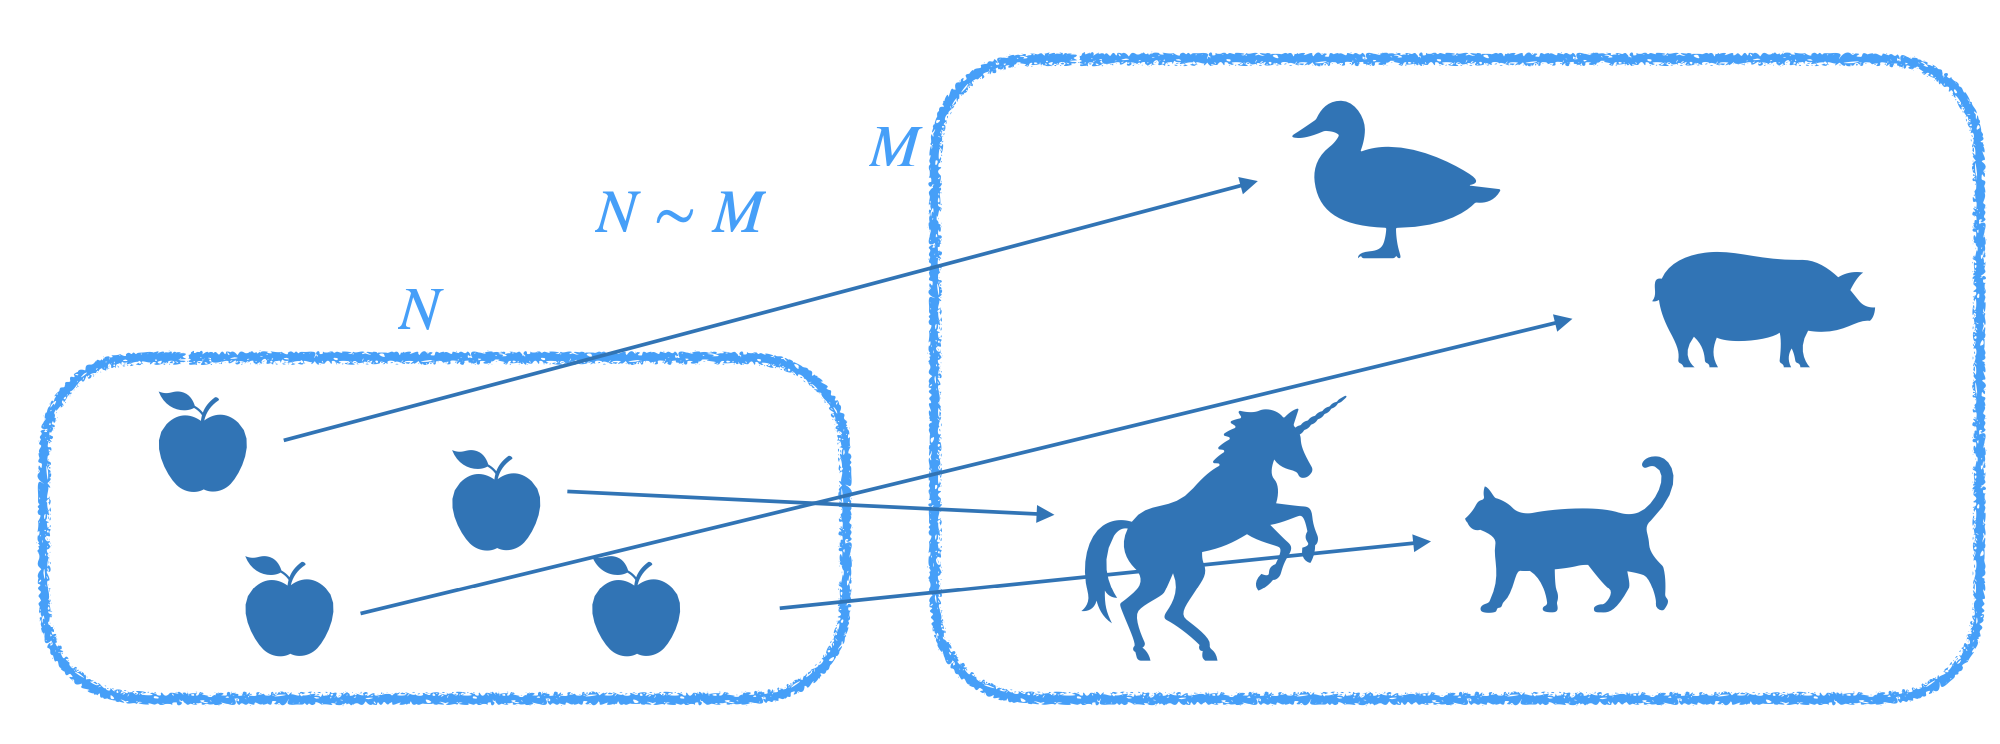
\includegraphics[width=0.75\linewidth]{pictures/2-Bijektion} 

}

\caption{Gleichmächtigkeit von Mengen}\label{fig:Bijektion}
\end{figure}

Diese Relation ist eine Äquivalenzrelation, also symmetrisch, reflexiv und transitiv. Damit können Äquivalenzklassen gebildet werden, die die Mächtigkeit der Menge angeben. \(4\) ist dann der Bezeichner für die Äquivalenzklasse von vierelementigen Mengen. Die Addition \(n+k\) entspricht dann der Mächtigkeit der Vereinigungsmenge von Mengen mit den Mächtigkeiten \(n\) und \(k\), vgl. Abbildung \ref{fig:Vereinigung}.

\begin{figure}

{\centering 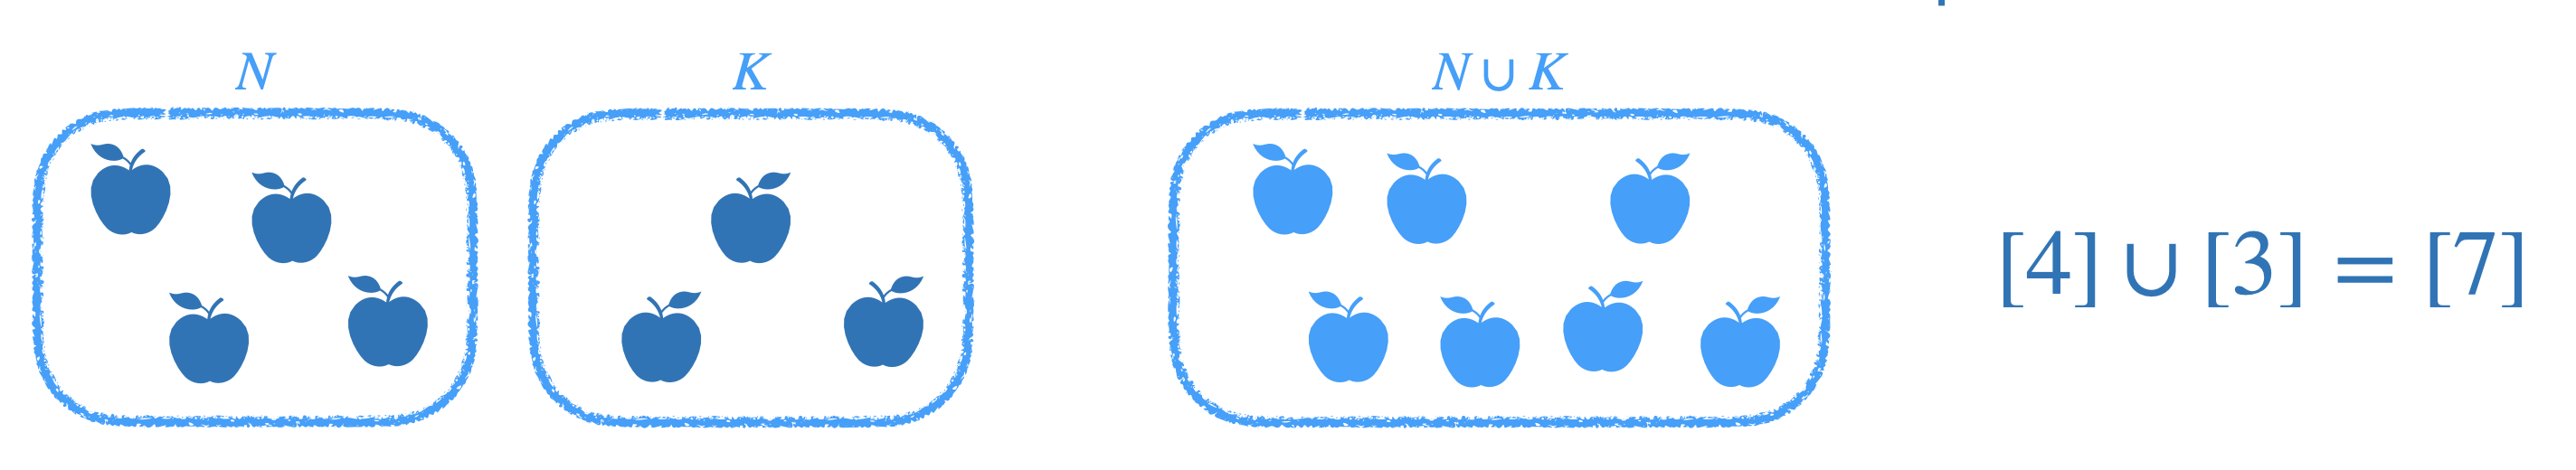
\includegraphics[width=0.9\linewidth]{pictures/2-Vereinigung} 

}

\caption{Additionsergebnis als Äquivalenzklasse der Vereinigungsmenge}\label{fig:Vereinigung}
\end{figure}

\subsection{Ganze Zahlen}\label{ganze-zahlen}

Da innerhalb der natürlichen Zahlen noch nicht beliebig subtrahiert werden darf, stehen auch keine negativen Zahlen als Ergebnisse zur Verfügung. Um dennoch das Ergebnis bspw. der Aufgabe \(2-7\) »definieren« zu können, bietet sich erneut eine \textbf{Äquivalenzrelation} über die »Differenzengleichheit« an. Konkret lässt sich für \(k,l,m,n\in\mathbb{N}\) sagen:
\((k,l)\sim (m,n):\Leftrightarrow k+n=l+m\)
Das heißt z.~B., dass die Zahlenpaare \((2,7)\), \((0,5)\) und \((4,9)\) in Relation zueinander stehen, weil sie dieselbe »Differenz« haben (obwohl es die Differenz formal noch nicht gibt). Dies ermöglicht nun die Einführung des Bezeichners \(-5\) für die Äquivalenzklasse \([(0,5)]\).

Das Vorgehen ist \emph{verträglich} mit den bisherigen Regeln in \(\mathbb{N}\), d.~h. es führt nicht zu Widersprüchen, wenn etwa das Zahlenpaar \((7,4)\) betrachtet wird mit dem Repräsentanten-Bezeichner \(3\). Die Menge aller Äquivalenzklassen (bzw. deren Kurzbezeichner) ist nun \(\mathbb{Z}\).

Die Addition und Subtraktion zweier Zahlenpaare sind nun definierbar:

\begin{align}
(k, l) + (m, n) := (k + m, l + n)\\
(k, l) − (m, n) := (k, l) + (n, m)
\end{align}

Als Alternative bietet sich ein \textbf{axiomatisches Vorgehen} an, also dass die ganzen Zahlen mit der Addition als abelsche Gruppe definiert werden -- bedeutsam ist hier insbesondere die Existenz eines Inversen zu jeder Zahl.

\subsubsection{Permanenzprinzip und Permanenzreihen}\label{permanenzprinzip-und-permanenzreihen}

Wie bereits erwähnt, führen die neu eingeführte Addition und Subtraktion in \(\mathbb{Z}\) nicht zu Konflikten mit den bisherigen analogen Operationen in \(\mathbb{N}\). Dies wird über das \textbf{\emph{Permanenzprinzip}} gefordert, nach dem neue Theorien (z.~B. das Rechnen mit negativen Zahlen) soweit wie möglich verträglich sein müssen mit bisherigen Theorien (z.~B. das Rechnen mit positiven Zahlen).

Sichtbar gemacht werden kann dieses Prinzip über \textbf{\emph{Permanenzreihen}}. Dies ist insbesondere dann hilfreich, wenn für bestimmte Rechenoperationen keine geeigneten realen Veranschaulichungen existieren. Ein typisches Beispiel hierfür ist die Multiplikation zweier negativer Zahlen. Kann die Multiplikation einer natürlichen Zahl (erster Summand) mit einer negativen Zahl (zweiter Summand) außermathematisch noch als mehrfache Verschuldung aufgefasst und die Vertauschung von erstem und zweitem Summanden über das Kommutativgesetz innermathematisch erklärt werden, bietet die Multiplikation zweier negativer Zahlen keine so naheliegende Interpretation. Abbildung \ref{fig:Permanenz} stellt eine Permanenzreihe dar, anhand derer die Rechnung \((-3)\cdot (-5)\) erklärt werden kann.

\begin{figure}

{\centering 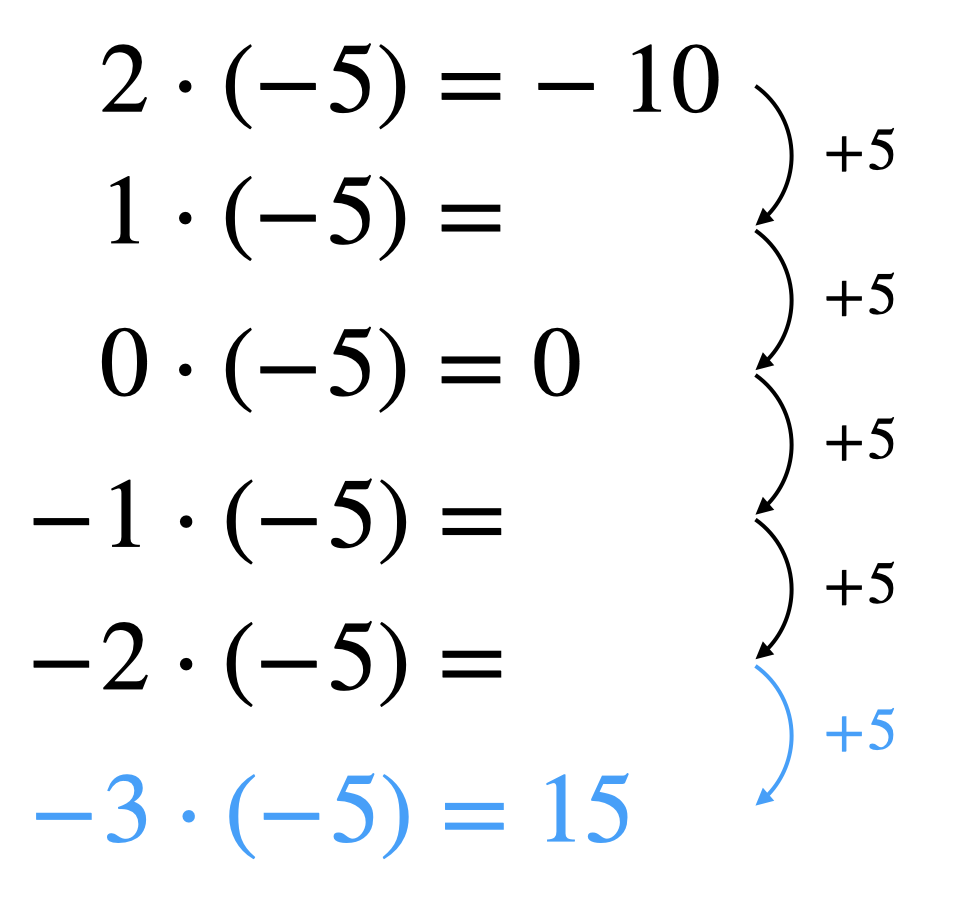
\includegraphics[width=0.3\linewidth]{pictures/2-Permanenz} 

}

\caption{Permanenzreihe zur Multiplikation zweier negativer Zahlen}\label{fig:Permanenz}
\end{figure}

Entscheidend ist beim Aufstellen von Permanenzreihen jedoch, dass der Übergang von einer Zeile zur nächsten auf einem entsprechenden Rechengesetz beruht. Im Abbildung \ref{fig:Permanenz} ist dies das Distributivgesetzt \((a-1) \cdot b = a \cdot b - b\). Varnachlässigt man die Existenz einer Übergangsregel, lassen sich plausibel erscheinende Muster fortsetzen (wie \(0^3 = 0\), \(0^2 = 0\), \(0^1 = 0\)), die dann allerdings zu falschen Schlussfolgerungen (\(0^0 = 0\)) führen. Im dargestellten Beispiel kann die Übergangsregel \(a^{m-1} = a^m : a\) wegen \(a = 0\) nicht angewandt werden.

\subsubsection{Ableitungen für den Lernpfad}\label{ableitungen-fuxfcr-den-lernpfad}

Aus all den bisherigen Überlegungen auf der formalen Ebene lassen sich für den Unterricht zentrale Fachinhalte ableiten:

\textcolor{formalColor}{Ganze Zahlen können über Zahlenpaare aus den natürlichen Zahlen oder als »Gegenzahlen« der natürlichen Zahlen entwickelt werden.}

\begin{itemize}
\tightlist
\item
  \textcolor{formalColor}{Natürliche Zahlen sind als Teilmenge in die ganzen Zahlen eingebettet.}
\item
  \textcolor{formalColor}{Die Subtraktion natürlicher Zahlen $m-n$ mit $n > m$ ist nun lösbar.}
\item
  \textcolor{formalColor}{Die Rechenregeln werden erweitert, wobei die bekannten weiter gelten. Die wird über das Permanenzprinzip begleitet, bei der Herleitung von Rechenregeln bietet sich die Nutzung von Permanenzreihen an.}
\end{itemize}

\subsection{Rationale Zahlen}\label{rationale-zahlen}

In fachlich analoger Weise lassen sich auch die rationalen Zahlen über Äquivalenzrelationen einführen. Dann fordert die »Quotientengleichheit«, dass für \(k,l,m,n\in\mathbb{N}\) mit \(l,n\neq 0\) gilt: \((k,l)\sim (m,n):\Leftrightarrow k\cdot n=l\cdot m\). Die Äquivalenzklasse \([(1,2)]\) kann dann mit \(\frac{1}{2}\) bezeichnet werden. Im Gegensatz zu den ganzen Zahlen ist es bei den rationalen Zahlen durchaus üblich, für dieselbe Zahl unterschiedliche Bezeichner zu verwenden, wie \(\frac{1}{2}\) oder \(\frac{5}{10}\). Fachmathematisch ist dies jedoch nicht relevant, also auch keine Diskussion auf der formalen Ebene (jedoch auf späteren Ebenen).

Aus Sicht der formalen Ebene lässt sich daher auch nicht ableiten, ob im Mathematikunterricht nach den natürlichen Zahlen zunächst die rationalen Zahlen (wie z.~B. in Deutschland) oder erst die ganzen Zahlen (wie z.~B. in Australien) eingeführt werden sollten. Innerhalb eines Zahlbereichs bietet jedoch die fachlogische Struktur Ansatzpunkte zur Gestaltung des Lernpfads, wie bei den negativen Zahlen dargestellt.

\section{Zum Nachbereiten}\label{mathematik-strukturieren-nachbereitung}

\begin{enumerate}
\def\labelenumi{\arabic{enumi}.}
\tightlist
\item
  Nutzen Sie verschiedene fachmathematische und fachdidaktische Quellen sowie Schulbücher, um fachlich zu klären, was »Terme« und »Gleichungen« sind.
\item
  Nutzen Sie Permanenzreihen, um weitere Rechengesetze nachzuvollziehen, z.~B. dass \(a^0 = 1\) (\(a\neq 0\)) und \(a^\frac{1}{2} = \sqrt{a}\) (\(a \geq 0\)) ist.
\item
  Wählen Sie eine Leitidee aus den Bildungsstandards aus und nennen Sie innerhalb dieser Begriffe, Zusammenhänge und Verfahren, die im Mathematikunterricht behandelt werden.
\end{enumerate}

\chapter{Grundvorstellungen}\label{grundvorstellungen}

\begin{quote}
\textbf{Ziele}

\begin{itemize}
\tightlist
\item
  Sie können die Grundvorstellungsidee beschreiben und wissen über deren Bedeutung für den Mathematikunterricht.
\item
  Ihnen ist bewusst, dass Grundvorstellungen i.~d.~R. zu Begriffen (Objekten und Operationen) existieren.
\item
  Sie kennen Grundvorstellungen zu einzelnen mathematischen Begriffen.
\end{itemize}

\textbf{Material}

\begin{itemize}
\tightlist
\item
  Folien zum Kapitel 3 (\href{files/Stoffdidaktik2024-03-Grundvorstellungen.pdf}{pdf}, \href{files/Stoffdidaktik2024-03-Grundvorstellungen.key}{Keynote})
\end{itemize}
\end{quote}

\section{Begriffsklärung}\label{grundvorstellungen-begriffsklaerung}

\subsection{Grundvorstellungsidee}\label{grundvorstellungsidee}

Als Sie zu Beginn Ihres Mathematikstudiums die Peano-Axiome zur Definition der natürlichen Zahlen \(\mathbb{N}\) kennengelernt haben, konnten Sie dies wahrscheinlich -- trotz der Neuigkeit der formalen Beschreibung -- derart mit Ihrer Lebenswelterfahrung in Verbindung bringen, dass natürliche Zahlen abgezählt werden können, also dass damit z.~B. die Platzierungen eines Wettrennens durchnummeriert werden können.

\begin{quote}
\textbf{Peano-Axiome} (\citeproc{ref-WikiPeano}{Wikipedia, 2021a})

\begin{enumerate}
\def\labelenumi{\arabic{enumi}.}
\tightlist
\item
  \(0\) ist eine natürliche Zahl.
\item
  Jede natürliche Zahl \(n\) hat eine natürliche Zahl \(n'\) als Nachfolger.
\item
  \(0\) ist kein Nachfolger einer natürlichen Zahl.
\item
  Natürliche Zahlen mit gleichem Nachfolger sind gleich.
\item
  Enthält die Menge \(X\) die \(0\) und mit jeder natürlichen Zahl \(n\) auch deren Nachfolger \(n'\), so bilden die natürlichen Zahlen eine Teilmenge von \(X\).
\end{enumerate}
\end{quote}

Dieser \textbf{Bezug auf eine bekannte Handlung} ist wesentlich dafür, dass die Definition und damit der Begriff der natürlichen Zahlen für Sie mit einem Sinn behaftet ist. Innerhalb dieser \emph{ordinalen Sichtweise} natürlicher Zahlen helfen nun geeignete\footnote{\emph{Geeignet} heißt in diesem Fall, dass sich die Kernaussage des Begriffs in der Repräsentation wiederfindet. Im Ordinalzahlaspekt ist dies v.~a. die Reihung von Zahlen. Was dabei (noch) nicht relevant ist, ist zum Beispiel die exakte Messbarkeit, wie man sie etwa auf dem Zahlenstrahl repräsentiert.} \textbf{Repräsentationen} dabei, sich Rechenoperationen vorstellen und sie \textbf{operativ}\footnote{\emph{Operativ} heißt hier zum Beispiel, dass Sie zu einer Aufgabe wie \(2+7\) Nachbaraufgaben (\(2+8\)), Umkehraufgaben (\(7-2\)), Platzhalteraufgaben (\(2+\boxed{\phantom{5}}=7\)) usw. aufstellen und lösen können.} auszuführen zu können, also bspw. das Addieren als ein Weiterzählen aufzufassen (siehe Abbildung \ref{fig:Addition}).\index{Natürliche Zahlen|)}

\begin{figure}

{\centering 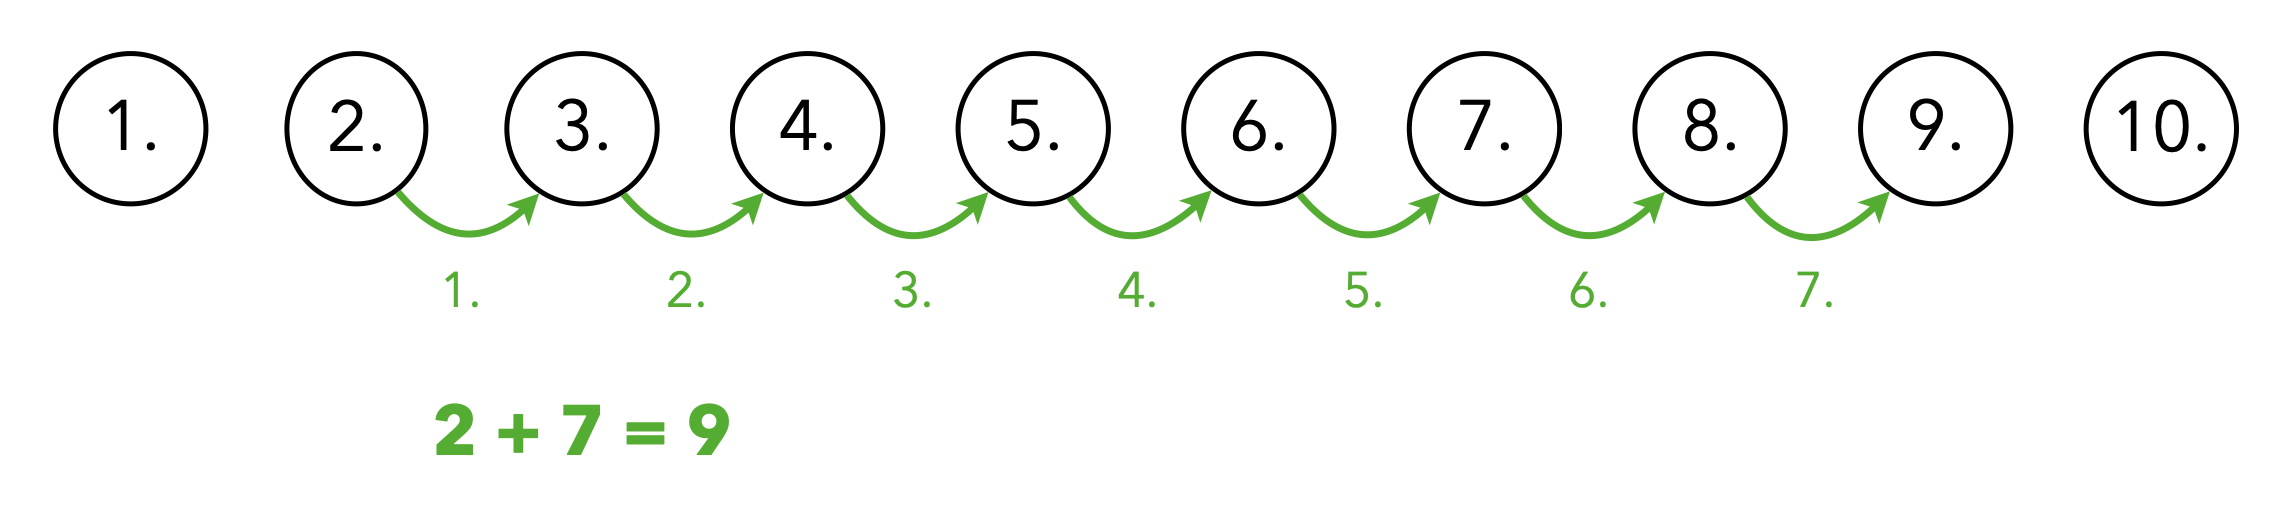
\includegraphics[width=0.75\linewidth]{pictures/4-Addition} 

}

\caption{Additionsaufgabe im ordinalen Zahlaspekt}\label{fig:Addition}
\end{figure}

Mit der Fähigkeit der Verknüpfung des mathematischen Begriffs und der Lebenswelt ist also eine \textbf{Anwendung des Begriffs auf die Wirklichkeit} möglich, insbesondere in Modellierungsprozessen. Dabei sind beide Richtungen relevant: Von der Realsituation zur Mathematik und von der Mathematik zur Realität.

Ziel des Mathematikunterrichts sollte es nun sein, für alle relevanten mathematischen Begriffe ein derartiges Verständnis aufzubauen, was auch heißt, verschiedene Vorstellungen zu einem Begriff zu vermitteln. Nach vom Hofe (\citeproc{ref-Hofe:1995}{1995, 97~f.}, Hervorhebung durch H.E.) ergibt sich daraus eine Orientierung an Grundvorstellungen im Mathematikunterricht:

\begin{definition}[Grundvorstellungen]
\protect\hypertarget{def:Grundvorstellungen}{}\label{def:Grundvorstellungen}

Die \textbf{Grundvorstellungsidee}\index{Grundvorstellung|textbf}\index{Grundvorstellungsidee|see{Grundvorstellung}} beschreibt \textbf{Beziehungen zwischen mathematischen Inhalten und} dem Phänomen der \textbf{individuellen Begriffsbildung}. In ihren unterschiedlichen Ausprägungen charakterisiert sie mit jeweils unterschiedlichen Schwerpunkten insbesondere drei Aspekte dieses Phänomens:

\begin{itemize}
\tightlist
\item
  Sinnkonstituierung eines Begriffs durch \textbf{Anknüpfung an} bekannte \textbf{Sach- oder Handlungszusammenhänge} bzw. \textbf{Handlungsvorstellungen},\index{Grundvorstellung!Sinnkonstituierung|textbf}
\item
  Aufbau entsprechender (visueller) \textbf{Repräsentationen bzw. »Verinnerlichungen«}, die \textbf{operatives Handeln} auf der Vorstellungsebene ermöglichen,\index{Grundvorstellung!Repräsentation|textbf}
\item
  Fähigkeit zur Anwendung eines Begriffs auf die Wirklichkeit durch \textbf{Erkennen der} entsprechenden \textbf{Struktur in Sachzusammenhängen} oder durch \textbf{Modellieren} des Sachproblems \textbf{mit Hilfe der mathematischen Struktur}.\index{Grundvorstellung!Modellierung|textbf}
\end{itemize}

\end{definition}

\subsection{Ausdifferenzierung}\label{ausdifferenzierung}

Weiterhin unterscheidet vom Hofe (\citeproc{ref-vomHofe2014}{2014}) zwischen \textbf{primären}\index{Grundvorstellung!primäre Grundvorstellung} und \textbf{sekundären}\index{Grundvorstellung!sekundäre Grundvorstellung} Grundvorstellungen, abhängig von der Erfahrungswelt der Handlungen. Während sich primäre Grundvorstellungen auf reale Handlungserfahrungen stützen (z.~B. mit Steckwürfeln in der Arithmetik), entstammen sekundäre Grundvorstellungen aus den Handlungen mit bereits im Mathematikunterricht aufgebauten Repräsentationen (z.~B. Operationen auf dem Zahlenstrahl).

Einige Quellen unterscheiden zwischen \textbf{Aspekten} und \textbf{Grundvorstellungen}. Nach Greefrath et al. (\citeproc{ref-Greefrath2016}{2016, S. 17}) ist ein »Aspekt eines mathematischen Begriffs {[}\ldots{]} ein Teilbereich des Begriffs, mit dem dieser fachlich
charakterisiert werden kann«, während »eine Grundvorstellung zu einem mathematischen Begriff {[}\ldots{]} eine inhaltliche Deutung des Begriffs {[}ist{]}, die diesem Sinn gibt.« Im oben angebrachte Beispiel entspräche die Definition der natürlichen Zahlen über die Peano-Axiome dem \emph{Ordinalzahlaspekt}, der mit der Grundvorstellung verbunden ist, dass die natürlichen Zahlen mit \(0\) beginnend eine feste Reihenfolge beschreiben. Da jedoch nicht alle Quellen diese Unterscheidung so präzise vornehmen und es auch teils zu Vermischungen kommt, soll diese (auf theoretischer Ebene relevante) Diskussion hier in der Stoffdidaktik-Veranstaltung nicht weiter von Relevanz sein. Für Ihre Unterrichtsgestaltung ist insbesondere relevant, dass sie einen \textbf{aspektreichen bzw. an vielfältigen Grundvorstellungen} orientierten Umgang mit Begriffen anstreben. Auch wenn Sie nicht unmittelbar und sofort jeweils alle Aspekte eines Begriffs im Unterricht ansprechen werden, hilft Ihnen das Wissen über den Aspektreichtum in der Unterrichtsplanung für die Ausbildung eines umfassenden Begriffsverständnisses.

Entsprechend ihrer Definition werden Grundvorstellungen für \textbf{Begriffe} erarbeitet -- hinsichtlich der Arten mathematischen Wissens (vgl. Abschnitt \ref{arten-mathematischen-wissens}) also anscheinend nicht für Zusammenhänge und Verfahren. Jedoch können Grundvorstellungen zu einem Begriff sowohl hinsichtlich des \emph{Objekts} an sich bestehen, als auch hinsichtlich der \emph{Operationen} mit diesem Begriff. Das Addieren ist beispielsweise im Ordinalzahlaspekt eine Operation, verbunden mit der Grundvorstellung des Weiterzählens. Insofern können auch Zusammenhänge und Verfahren durchaus mit Grundvorstellungen verknüpft werden, sofern der Fokus auf dem Operieren mit den in ihnen enthaltenen Begriffen liegt.

Die in Definition \ref{def:Grundvorstellungen} dargestellte Grundvorstellungsidee hat einen \textbf{normativen}\index{Grundvorstellung!normativ|textbf} Charakter, d.~h. es wird davon ausgegangen, dass (aus professioneller Sicht der Mathematikdidaktik) zu mathematischen Begriffen bestimmte Grundvorstellungen identifiziert werden können, die es im Unterricht zu vermitteln gilt. Oder anders gefragt: »Welche Grundvorstellungen sind zur Lösung des Problems aus der Sicht des Lehrenden adäquat?« (\citeproc{ref-Hofe:1995}{vom Hofe, 1995, S. 106}). Diese Sichtweise wird durch eine \textbf{deskriptive}\index{Grundvorstellung!deskriptiv|textbf} Perspektive ergänzt: »Welche individuellen Vorstellungen lassen sich im Lösungsversuch des Schülers erkennen?« (\citeproc{ref-Hofe:1995}{vom Hofe, 1995, S. 107}). Diese über empirische Untersuchungen zu ermittelnden Vorstellungen sind das, was sich Schülerinnen und Schüler \emph{tatsächlich} unter einem Begriff vorstellen, wozu ggf. auch typische \emph{Fehlvorstellungen}\footnote{Mit \emph{Fehlvorstellungen} sind hier individuelle Vorstellungen der Schülerinnen und Schüler gemeint, die mathematisch nicht tragfähig und daher aus fachlicher Perspektive fehlerhaft sind. So ist etwa die Vorstellung, dass Multiplizieren immer vergrößert, in den Natürlichen Zahlen tragfähig (und damit eine Grundvorstellung), in den Bruchzahlen jedoch nicht mehr tragfähig und wird dort dann zur Fehlvorstellung. Neben \emph{Fehlvorstellungen} können weitere individuelle Vorstellungen \emph{Alltagsvorstellungen}, \emph{Präkonzepte} o.~ä. sein (siehe auch \citeproc{ref-Schecker2018}{Schecker et al., 2018, 11~f.}).} gehören können. Kenntnisse darüber sind für Lehrkräfte ungemein wichtig, um Ergebnisse von Schülerinnen und Schülern interpretieren und einordnen zu können und dann ggf. entsprechende Hilfsangebote zu machen. Dies entspricht dann einer \textbf{konstruktiven}\index{Grundvorstellung!konstruktiv|textbf} Perspektive auf Grundvorstellungen: »Worauf sind etwaige Divergenzen zurückzuführen, und wie lassen sich diese beheben?« (\citeproc{ref-Hofe:1995}{vom Hofe, 1995, S. 107}).

\section{GV und Stoffdidaktik}\label{gv-und-stoffdidaktik}

Im Rahmen dieser Veranstaltung, insbesondere den von Ihnen ausgearbeiteten Seminarthemen, wird der Schwerpunkt auf \emph{normative} Grundvorstellungen gelegt, was der \textcolor{semanticColor}{semantischen Ebene} des \hyperref[tab:fragen-ebenen]{Vier-Ebenen-Ansatzes} zugeordnet werden kann, weil die mathematischen Begriffe hier mit einem Sinn versehen werden. Die \emph{deskriptive} und \emph{konstruktive} Perspektive sind dagegen der \textcolor{empiricColor}{empirischen Ebene} zuzuordnen, da hier individuelle Vorstellungen der Schülerinnen und Schüler von Relevanz sind. Dies betrifft insbesondere auch das Potenzial, (ggf. mathematisch unvollständige) individuelle Vorstellungen aufzugreifen bei der Ausbildung von (normativ erwünschten) Grundvorstellungen.

Das Identifizieren von Grundvorstellungen zu einem Begriff ist, genau wie bei den \hyperref[fundamentale-ideen]{Fundamentalen Ideen}, Aufgabe der mathematikdidaktischen Forschung (ein Modell dafür findet man bei \citeproc{ref-Salle2021}{Salle \& Clüver, 2021}). Als Lehrkraft profitieren Sie von diesen Ergebnissen und nutzen sie für Ihre stoffdidaktische Analyse.

Im Gegensatz zu den fundamentalen Ideen, die ihren Ursprung in der \emph{Sachstruktur des mathematischen Inhalts} haben, fokussieren die Grundvorstellungen stärker auf den Sinn des fachlichen Begriffs \emph{für das Individuum}. Grundvorstellungen beziehen sich auf spezifische Begriffe und Operationen mit Begriffen, während fundamentale Ideen größere, themenübergreifende Leitlinien für die Stoffauswahl und -strukturierung bilden.

Für die Unterrichtsplanung und -durchführung ist neben der Frage, \emph{welche} Grundvorstellungen von Relevanz sind (Spezifizieren im Vier-Ebenen-Ansatz) vor allem interessant, \emph{wie} diese ausgebildet werden können (Strukturieren im Vier-Ebenen-Ansatz). Letzteres wird u.~a. in den nächsten Kapiteln näher beleuchtet.

\section{Beispiele}\label{beispiele}

\subsection{Natürliche Zahlen}\label{natuxfcrliche-zahlen-1}

Betrachten Sie folgenden (fiktiven) Zeitungsartikel:\index{Natürliche Zahlen|(}

\begin{quote}
\textbf{\emph{Harlequin erneut auf dem 1. Platz}}

\emph{Bei dem traditionellen Pferderennen am 15. Mai hat das Pferd Harlequin erneut gewonnen. Unter den 10 Pferden, die an den Start gingen, belegte es mit 21,3 Sekunden den 1. Platz. Damit war es fast 2 mal so schnell unterwegs wie das letzte Pferd, das ins Ziel kam. Karten für das nächste Rennen können unter 030 23125143 bestellt werden.}
\end{quote}

In dem Text tauchen Zahlen unter vielen Aspekten auf: Der \textbf{1.} Platz und \textbf{15.} Mai sind \textbf{Ordinalzahlen}, also Zahlen, die eine Ordnung beschreiben. Wie oben schon beschrieben, lassen diese sich fachmathematisch über die Peano-Axiome beschreiben und wenn mit ihnen gerechnet, entspricht z.~B. das Addieren dem \textbf{Weiterzählen}.

Die \textbf{10} Pferde stellen eine \textbf{Kardinalzahl} dar, also die Anzahl der Elemente einer Menge. Addiert man Kardinalzahlen, so müssen \textbf{Mengen vereinigt} werden, z.~B. anschaulich, indem man sie zusammen legt.

Die \textbf{21,3} Sekunden entsprechen einer \textbf{Maßzahl}, da diese Zahl die Funktion hat, etwas auszumessen (hier die Zeit). Das Addieren in diesem Aspekt entspräche dem \textbf{Aneinanderlegen}, z.~B. wenn zwei Längenangaben addiert werden.

Dass es \textbf{2} mal so schnell wird, enspricht einem \textbf{Operatoraspekt}, mit dem die Vielfachheit eines Vorganges beschrieben wird. Das Addieren ist hierin eine \textbf{Hinereinanderausführung} eines Vorganges.

Die Telefonnumer \textbf{030 23125143} wiederum erfüllt einen \textbf{Codierungsaspekt}. Sie hat im mathematischen Sinne keine Bedeutung, nur die Anordnung der Ziffern ist von Relevanz. Entsprechend kann innerhalb dieses Aspektes auch nicht addiert werden. Weitere Beispiele hierfür wären Postleitzahlen oder Identifikationsnummern.

Hinzu kommt noch der Aspekt der \textbf{Rechenzahl}. Informationen dazu sowie eine genauere Erläuterung der Zahlaspekte und damit verbundenen Operationen findet man z.~B. bei Krauthausen (\citeproc{ref-Krauthausen:2018}{2018, 43~ff.}).\index{Natürliche Zahlen|)}

\subsection{Bruchzahlen}\label{bruchzahlen}

Nachdem\index{Brüche|(} die Schülerinnen und Schüler ihr gesamte Vorschul- und Primarstufenzeit mit Natürlichen Zahlen verbracht haben, treten mit der Einführung von Bruchzahlen Umbrüche in den subjektiven Vorstellungen auf. Zum Beispiel sind folgende (vermeintlichen) Gesetzmäßigkeiten plötzlich \emph{nicht mehr} gültig:

\begin{itemize}
\tightlist
\item
  Das Produkt zweier Zahlen ist größer als die jeweiligen Faktoren.
\item
  Die Multiplikation kann als wiederholte Addition aufgefasst werden.
\item
  Jede Zahl hat genau einen Repräsentanten.
\item
  Je mehr Stellen eine Zahl hat, desto größer ist sie.
\end{itemize}

Die Bruchzahlen selbst besitzen nach Padberg \& Wartha (\citeproc{ref-Padberg:2017}{2017, 19~ff.}) folgende Aspekte:

\begin{itemize}
\tightlist
\item
  Bruch als \textbf{Anteil eines Ganzen} oder \textbf{mehrerer Ganzer}
  (z.~B. \(\frac{2}{3}\) als zwei Drittel einer Pizza oder je ein Drittel von zwei Pizzen),
\item
  Bruch als \textbf{Maßzahl}
  (z.~B. \(\frac{1}{4}\) Liter),
\item
  Bruch als \textbf{Operator}
  (z.~B. \(\frac{1}{5}\) von 250 €),
\item
  Bruch als \textbf{Verhältnis}
  (z.~B. \(\frac{2}{3}\) mit der Bedeutung \emph{2 von 3 Schüler/-innen tragen eine Brille}),
\item
  Bruch als \textbf{Quotient}
  (z.~B. \(\frac{3}{5}\) als Ergebnis bzw. andere Schreibweise von \(3:5\)),
\item
  Bruch als \textbf{Lösung einer linearen Gleichung}
  (z.~B. \(\frac{3}{5}\) als Lösung von \(5x = 3\)),
\item
  Bruch als \textbf{Skalenwert}
  (z.~B. \(\frac{3}{2}\) als Mitte zwischen \(1\) und \(2\) auf dem Zahlenstrahl),
\item
  \textbf{Quasikardinale Auffassung} von Brüchen
  (z.~B. \(\frac{3}{5}\) als 3 mal \(\frac{1}{5}\)).
\end{itemize}

Neben den Grundrechenoperationen führt auch das Vergleichen von Brüchen zu Grundvorstellungsumbrüchen. Hinzu kommen noch besondere Operationen mit Bruchzahlen wie das Erweitern und Kürzen.

Das Multiplizieren von Brüchen kann bspw. als Anteilsbildung (\(\frac{1}{5}\) mal \ldots{} heißt \(\frac{1}{5}\) \emph{von} \ldots) oder als Rechteckfläche aufgefasst werden (\citeproc{ref-Padberg:2017}{Padberg \& Wartha, 2017, 108~ff}), siehe Abbildung \ref{fig:Bruchmultiplikation}.

\begin{figure}

{\centering 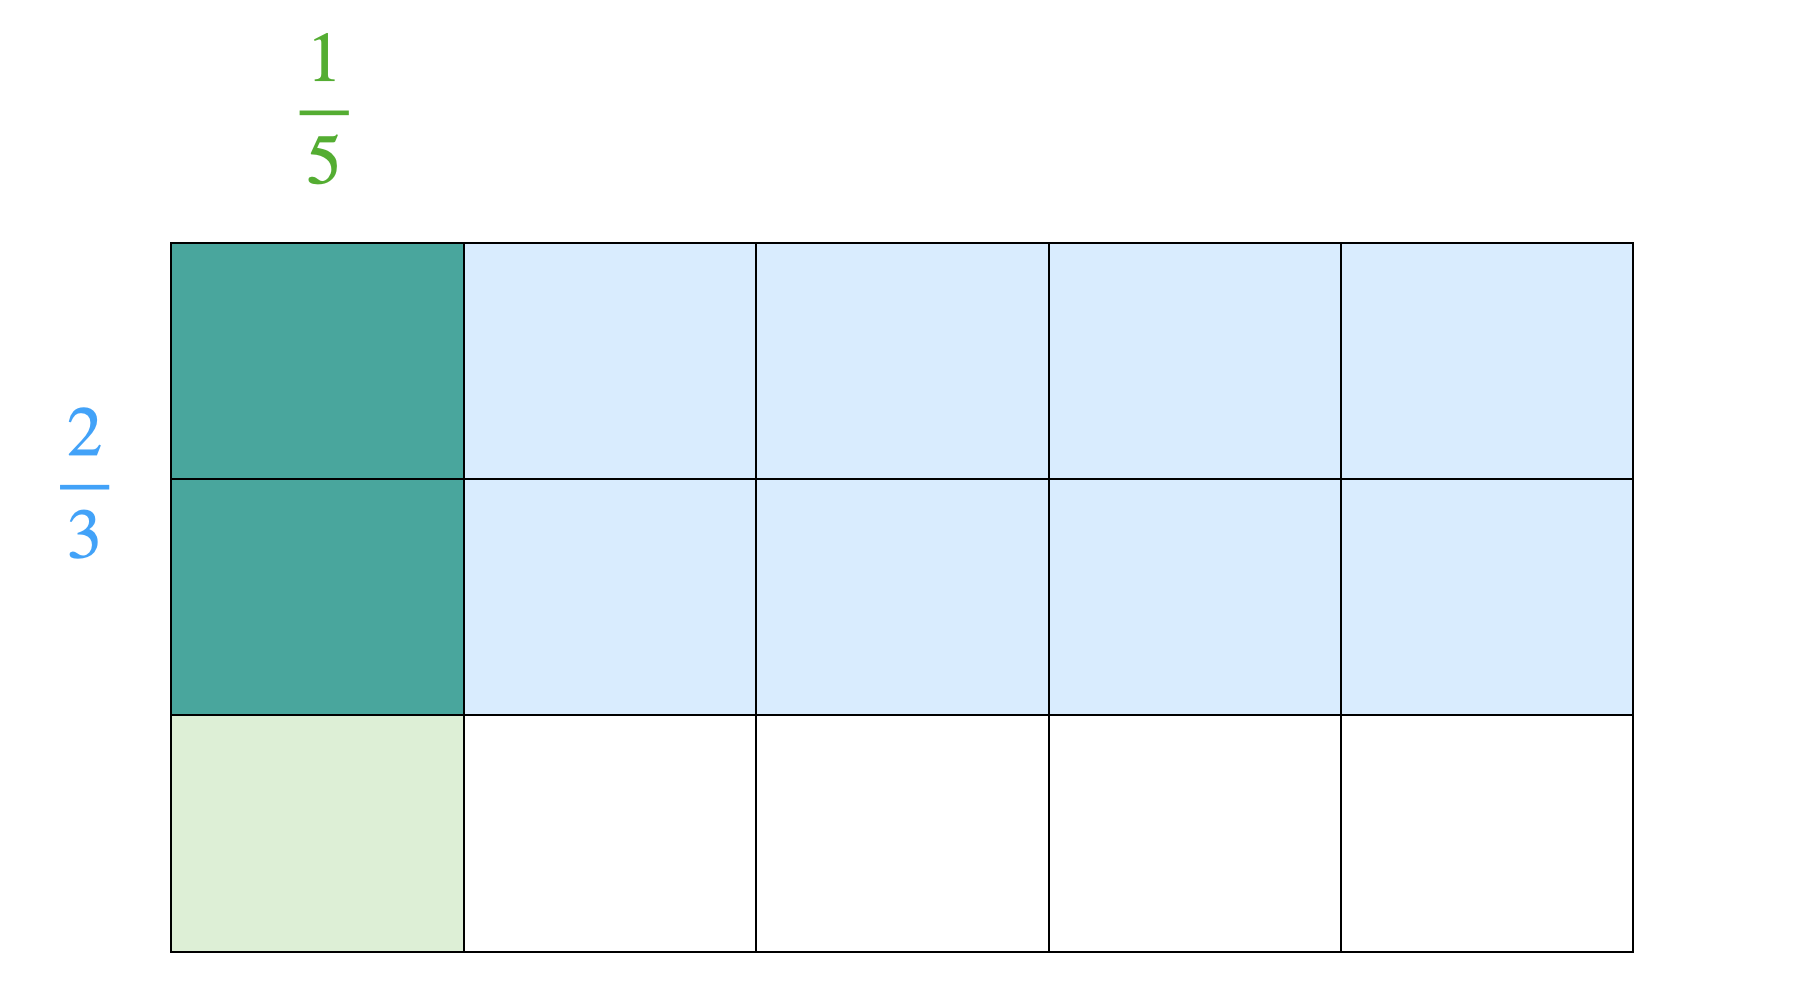
\includegraphics[width=0.5\linewidth]{pictures/4-Bruchmulti} 

}

\caption{Vorstellung von $\frac{1}{5} \cdot \frac{2}{3}$ als Rechteckfläche}\label{fig:Bruchmultiplikation}
\end{figure}

All dies zeigt, dass Brüche behutsam unterrichtet werden sollten und von einer rein kalkülorientierten Behandlung unbedingt abgesehen werden muss, da diese den nachhaltigen Lernerfolg deutlich mindert.\index{Brüche|)}

\subsection{Negative Zahlen}\label{negative-zahlen}

Aufbauend auf die in Abschnitt \ref{beispiel-negative-zahlen} erfolgte Diskussion zur \textcolor{formalColor}{formalen Ebene} von negativen Zahlen, soll zu diesen nun die Grundvorstellungsidee auf der \textcolor{semanticColor}{semantischen Ebene} diskutiert werden.

Die Einführung negativer Zahlen ist für Schülerinnen und Schüler mit zahlreichen Schwierigkeiten verbunden (\citeproc{ref-vomHofe2014a}{vom Hofe \& Hattermann, 2014}). Diese sind eigentlich auf der \textcolor{empiricColor}{empirischen Ebene} der stoffdidaktischen Analyse angesiedelt, sollen aber hier wegen ihrer Nähe zu den Grundvorstellungen schon einmal erwähnt werden.

\begin{itemize}
\tightlist
\item
  So bestehen etwa für das \textbf{Minus-Zeichen vielfältige Interpretationsmöglichkeiten} als \textbf{Vorzeichen} (z.~B. in der Rechnung \(-5+2\)), als \textbf{Rechenzeichen} (z.~B. in der Rechnung \(7-2\)) oder als \textbf{Inversionszeichen} (z.~B. bei der Darstellung \(-a\) als Gegenzahl für \(a\)).
\item
  Der in den natürlichen Zahlen vorhandene \textbf{Kardinalzahlaspekt} (dass die Zahl die Mächtigkeit einer Menge angibt), ist in den negativen Zahlen \textbf{nicht mehr tragfähig} (es existiert keine \(-4\)-elementige Menge). Auch der \textbf{Ordinalzahlaspekt} (dass die Zahl eine Position angibt) ist nur \textbf{eingeschränkt tragfähig} (eine \(-4\)-te Position bedarf vielfältiger Zwischeninterpretationen). Der \textbf{Maßzahlaspekt} (z.~B. über die Angabe einer Zahl auf dem Zahlenstrahl) dagegen ist auf die negativen Zahlen \textbf{erweiterbar}.
\item
  Die \textbf{Ordnungsrelation} wird häufig \textbf{fehlinterpretiert} über eine spiegelbildliche Interpretation (z.~B. kann fälschlicherweise \(-5>-3\) angenommen werden). Eine Ursache kann hier darin liegen, dass die Ordnungsrelation zuvor über die Mächtigkeit von Mengen hergestellt wurde, was nun nicht mehr möglich ist.
\end{itemize}

Gegenüber den natürlichen Zahlen sind also im Umgang mit negativen Zahlen einige Grundvorstellungsumbrüche zu absolvieren. Als normativ auszubildende Grundvorstellungen fassen vom Hofe \& Hattermann (\citeproc{ref-vomHofe2014a}{2014}) für rationale Zahlen (als Obermenge positiver und negativer Zahlen) zusammen:

\begin{itemize}
\tightlist
\item
  Rationale Zahlen als \textbf{relative Zahlen bezüglich einer fest gewählten Vergleichsmarke}: Dies ist etwa bei Etagen-Angaben, Temperaturen oder der Position über/unter dem Wasserspiegel der Fall. Gerade bei Temperaturen kann die Beliebigkeit der Vergleichsmarke (0~°C) gut diskutiert werden, da etwa andere Temperaturskalen (°F, K) eine andere Vergleichsmarke gewählt haben.
\item
  Rationale Zahlen als \textbf{Gegensätze}: Diese Vorstellung wird z.~B. sichtbar, wenn über Guthaben und Schulden gesprochen wird. Hat man 5~€ Schulden, so ist dies der Gegensatz von 5~€ Guthaben. Die Vergleichsmarke (0~€) ist hier nicht beliebig gewählt, sondern natürlicherweise über »weder Guthaben noch Schulden« gegeben. Auch der Betrag einer Zahl kann in dieser Vorstellung besonders gut verstanden werden.
\item
  Rationale Zahlen als \textbf{Richtungen}: Negative Zahlen beschreiben in dieser Vorstellung die entgegengesetzte Richtung der positiven Zahlen. Dies ist z.~B. bei der Verwendung von Koordinatensystemen der Fall, oder ganz allgemein bei der Zahlengeraden.
\item
  Rationale Zahlen als \textbf{Zustände und Zustandsänderungen}: In dieser Vorstellung bieten rationale Zahlen nicht nur die Möglichkeit, einen Zustand (wie Guthaben oder Schulden) zu beschreiben, sondern auch den Prozess der Änderung dieser Zustände (Erhalt von Guthaben, Erlass von Schulden, \ldots). Eine solche Vorstellung etwa ist nötig, um die verschiedenen Interpretationen des Minus-Zeichens nachvollziehen zu können.
\end{itemize}

Als bedeutsamste Repräsentation negativer Zahlen gilt die Zahlengerade. Diese stützt einerseits den Maßzahlaspekt und ermöglicht über die Darstellung von Punkten und Pfeilen (siehe Abbildung \ref{fig:Zahlengerade}) auch eine Interpretation in den verschiedenen Grundvorstellungen.

\begin{figure}

{\centering 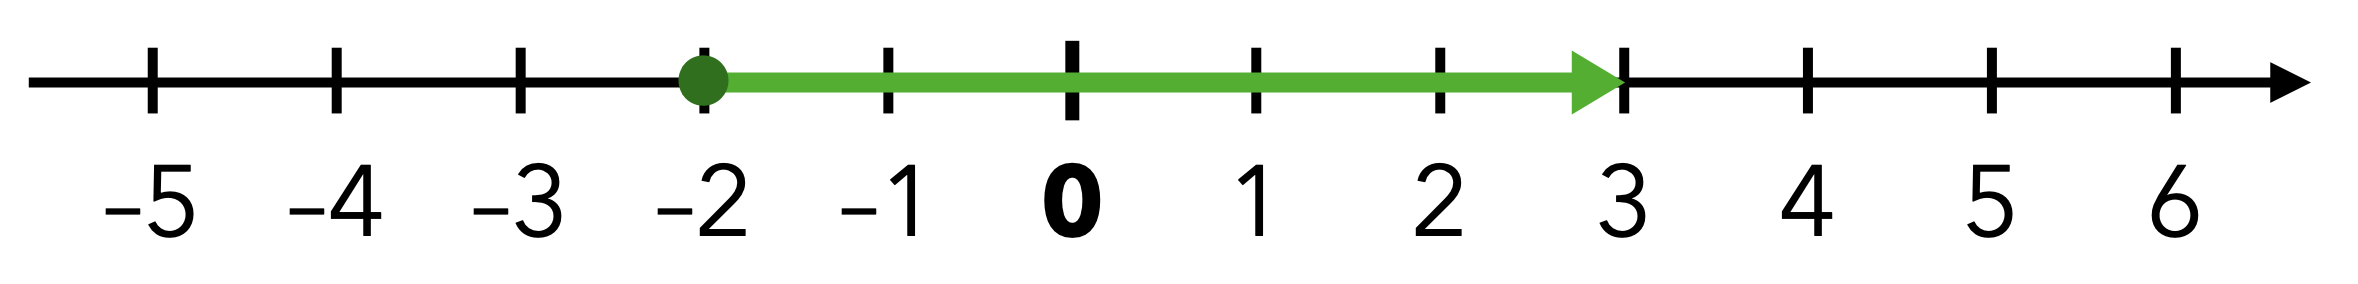
\includegraphics[width=0.75\linewidth]{pictures/4-Zahlengerade} 

}

\caption{Zahlengerade}\label{fig:Zahlengerade}
\end{figure}

Auch Operationen mit negativen Zahlen sind hierzu nun verständlich behandelbar:

\begin{itemize}
\tightlist
\item
  So kann das \textbf{Addieren/Subtrahieren} als Anlegen von Pfeilen, gerichtetes Weiter-/Zurückzählen oder als Subtraktion/Addition der Gegenzahl aufgefasst werden.
\item
  Das \textbf{Multiplizieren} kann bei der Multiplikation mit einer positiven Zahl als Streckung/Stauchung aufgefasst werden, die Multiplikation mit \(-1\) entspricht der Spiegelung an der Null und die Multiplikation mit einer beliebigen negativen Zahl ist eine Kombination aus beidem.
\item
  Der \textbf{Größenvergleich} ist nun über einen Lagevergleich auf der Zahlengeraden möglich, wobei weiter links liegende Zahlen immer kleiner sind als weiter rechts liegende.
\end{itemize}

Zusammenfassend lassen sich auf der semantischen Ebene folgende für den Lernpfad relevanten Zusammenhänge ableiten:

\begin{itemize}
\tightlist
\item
  \textcolor{semanticColor}{Rationale Zahlen sollten als relative Zahlen bezüglich einer fest gewählten Vergleichsmarke, als Gegensätze, als Richtungen sowie als Zustände und Zustandsänderungen aufgefasst werden können.}
\item
  \textcolor{semanticColor}{Die Zahlengerade ist eine wesentliche Repräsentation rationaler Zahlen, anhand derer auch die Operationen mit rationalen Zahlen sichtbar gemacht werden können.}
\end{itemize}

\section{Zum Nachbereiten}\label{grundvorstellungen-nachbereitung}

Bearbeiten Sie folgende Aufgaben entweder am Begriff \emph{Variable} oder am Begriff \emph{Term}. Als Quelle sei Weigand et al. (\citeproc{ref-Weigand2022}{2022}) zu empfehlen.

\begin{enumerate}
\def\labelenumi{\arabic{enumi}.}
\tightlist
\item
  Informieren Sie sich über die Grundvorstellungen zum gewählten Begriff.
\item
  Arbeiten Sie heraus, inwiefern die Aspekte der Grundvorstellungsidee erfüllt werden, d.~h.

  \begin{itemize}
  \tightlist
  \item
    stellen Sie die Sinnhaftigkeit des Begriffs durch mögliche Handlungserfahrungen dar,
  \item
    finden Sie geeignete Repräsentationen, anhand derer operatives Handeln ermöglicht wird und
  \item
    beschreiben Sie mögliche Modellierungsprozesse des Begriffs mithilfe der gewählten Grundvorstellung.
  \end{itemize}
\item
  Diskutieren Sie, ob es sich um primäre oder sekundäre Grundvorstellungen handelt.
\end{enumerate}

\chapter{Kernideen und Kontexte}\label{kernideen-und-kontexte}

\begin{quote}
\textbf{Ziele}

\begin{itemize}
\tightlist
\item
  Sie kennen das Konzept von Kernideen als das Wesen des Lerngegenstands.
\item
  Sie kennen Kernideen zu einzelnen Lerngegenständen.
\item
  Sie können gegebene Kontexte zu Lerngegenständen hinsichtlich ihrer Sinnstiftung beurteilen.
\item
  Sie sind sich der Möglichkeiten und Bedeutung horizontaler und vertikaler Mathematisierung bewusst.
\end{itemize}

\textbf{Material}

\begin{itemize}
\tightlist
\item
  Folien zum Kapitel 4 (\href{files/Stoffdidaktik2024-04-KernideenUndKontexte.pdf}{pdf}, \href{files/Stoffdidaktik2024-04-KernideenUndKontexte.key}{Keynote})
\end{itemize}
\end{quote}

\section{Begriffsklärung Kernidee/-frage}\label{kernidee-begriffsklaerung}

\textbf{Kernideen} haben die Aufgabe, den Lernpfad zu leiten und dabei das \emph{Wesen} des neuen Lerngegenstands sichtbar zu machen. Sie müssen dabei sowohl aus objektiver (also mathematischer) Perspektive tragfähig sein, als auch aus subjektiver Perspektive für die Schülerinnen und Schüler greifbar werden können. Kernideen bieten damit im \emph{Vorfeld} des Lernpfades eine Orientierung und im \emph{Nachgang} des Lernpfades eine Reflexionsmöglichkeit über den Lerngegenstand.\footnote{Der Begriff der Kernidee ist geprägt worden über das Dialogische Lernen nach Gallin und Ruf, spricht dort jedoch vorwiegend die Vorschauperspektive an (vgl. \citeproc{ref-Leuders2011}{Leuders et al., 2011, S. 7}).} Um bei den Schülerinnen und Schülern Lernprozesse zu einem Lerngegenstand zu initiieren, werden die Kernideen ansprechend in Form von \textbf{Kernfragen} formuliert. Kernfragen sollten daher prinzipiell aus subjektiver Sicht formuliert sein und insbesondere adressieren, wie man selbst mit dem Lerngegenstand umgehen kann.

Am Beispiel des \emph{Funktionsbegriffs}\index{Funktionsbegriff} etwa besteht eine Kernidee darin, dass Funktionen den Zusammenhang zwischen zwei Größen beschreiben und damit auch vorhersagen können (vgl. auch Aspekte des Funktionsbegriffs in einem späteren Kapitel). Als Kernfrage formuliert: »Wie kann man die Beziehung zwischen zwei sich verändernden Größen beschreiben und wie kann man damit weitere Werte bestimmen?« (\citeproc{ref-Thiel-Schneider2018}{Thiel-Schneider, 2018, S. 49}).

In der \emph{Vorschauperspektive} heißt das, die »Kernidee in Frageform schließt an individuelle Vorerfahrungen, Zielperspektiven, Denk- und Handlungsmuster der Lernenden an und initiiert die Auseinandersetzung mit dem mathematischen Gegenstand in den Worten von Schülerinnen und Schülern« (\citeproc{ref-Leuders2011}{Leuders et al., 2011, S. 8}). In der \emph{Rückschauperspektive} dagegen können über die Kernidee (dann quasi als Antwort auf die Kernfrage) »eine allgemeine Problemstellung und die zu ihrer Bewältigung notwendigen mathematischen Konzepte benannt« werden (\citeproc{ref-Leuders2011}{Leuders et al., 2011, S. 8}).

\begin{definition}[Kernidee und Kernfrage]
\protect\hypertarget{def:Kernidee}{}\label{def:Kernidee}Eine \textbf{Kernidee}\index{Kernidee|textbf} beschreibt in wenigen Worten das Wesen eines Lerngegenstands, d.~h. sie beschreibt, was den Lerngegenstand aus formaler und semantischer Perspektive auszeichnet -- insbesondere in Abgrenzung zu thematisch ähnlichen Lerngegenständen.

Eine \textbf{Kernfrage}\index{Kernfrage|textbf} stellt die Kernidee in Frageform aus der Perspektive der Schülerinnen und Schüler dar.

Kernideen und Kernfragen verfolgen eine \textbf{\emph{Vorschauperspektive}}\index{Kernidee!Vorschauperspektive|textbf}, die der Orientierung und Initiierung der Auseinandersetzung mit dem neuen Lerngegenstand dient, sowie eine \textbf{\emph{Rückschauperspektive}}\index{Kernidee!Rückschauperspektive|textbf}, die es den Schülerinnen und Schülern ermöglicht, den Lerngegenstand einzuordnen.
\end{definition}

Bestandteil Ihrer stoffdidaktischen Analyse auf der \textcolor{concreteColor}{konkreten Ebene} wird es also sein, zum Lerngegenstand passende Kernideen zu identifizieren und in Form von Kernfragen zu formulieren. Hierzu kann Ihnen die Sinnkonstituierung der jeweiligen Grundvorstellungen dienlich sein (siehe Definition \ref{def:Grundvorstellungen}).

\section{Begriffsklärung Kontext}\label{kontexte-begriffsklaerung}

\textbf{Kontexte} sollen geeignet sein, sich dem Lerngegenstand exemplarisch zu nähern. Sie weisen damit immer eine Spezialisierung bzw. Konkretisierung des zu betrachtenden Lerngegenstands auf (denn nur so können die Schülerinnen und Schüler einen Zugang dazu finden) -- sollen aber so gestaltet sein, dass an Ihnen das Allgemeine erfahrbar ist (denn nur so kann es zu einer Beschäftigung mit der dahinterliegenden Mathematik kommen). Es wird dann auch von einem \emph{sinnstiftenden Kontext} gesprochen.

Leuders et al. (\citeproc{ref-Leuders2011}{2011, S. 4}, Hervorhebungen im Original) formulieren hierzu:

\begin{definition}[Sinnstiftender Kontext]
\protect\hypertarget{def:Kontext}{}\label{def:Kontext}

Ein \textbf{sinnstiftender Kontext}\index{Kontext|textbf} ist ein Ausschnitt einer inner- oder außermathematischen Welt, der folgende Anforderungen möglichst gut erfüllt:

\begin{itemize}
\tightlist
\item
  Er ist anschlussfähig an die Erfahrungen, Interessen und die Denk- und Handlungsmuster der Lernenden \textbf{(Lebensweltbezug)}.\index{Kontext!Lebensweltbezug|textbf}
\item
  Er ermöglicht es, authentische Fragen zu bearbeiten und dabei auch etwas über den Kontext zu lernen \textbf{(Kontextauthentizität)}.\index{Kontext!Kontextauthentizität|textbf}
\item
  Er ist problemhaltig und offen genug, um Lernende zum reichhaltigen Fragen und Erkunden anzuregen \textbf{(Reichhaltigkeit)}.\index{Kontext!Reichhaltigkeit|textbf}
\end{itemize}

\end{definition}

Um einer eingeschränkten Sichtweise vorzubeugen, sei gesagt: Der \emph{Lebensweltbezug} heißt nicht zwingend, dass es sich um einen \emph{Realitätsbezug} (im Sinne einer Modellierung) handeln muss. Dies ist zwar in vielen Fällen angebracht, aber auch eine innermathematische Anschlussfähigkeit kann für die Schülerinnen und Schüler ansprechend sein (und damit Bezug zu deren -- schulischen -- Leben herstellen).

Ein möglicher Kontext, über den die oben formulierte Kernfrage bei \emph{linearen Funktionen}\index{Lineare Funktion}\index{Funktionsbegriff!Lineare Funktion|see{Lineare Funktion}} erarbeitet werden kann, wäre die Beschreibung des Abbrennverhaltens einer Kerze (vgl. \citeproc{ref-Boeer2014}{Böer et al., 2014, 108~f}). Dieser ist für die Schülerinnen und Schüler aus dem Alltag bekannt (wenn auch nicht alltäglich). Authentisch und reichhaltig ist der Kontext dahingehend, dass die meisten Kerzen zylinderförmig sind und daher tatsächlich ein lineares Abbrennverhalten haben. Auch ist es durchaus von Interesse, die Zeit bis zum vollständigen Abbrennen einer Kerze abschätzen zu können (z.~B. bei einer \emph{Kerzenuhr}, vgl. \citeproc{ref-WikiKerze}{Wikipedia, 2022a}). Weiterhin können (später) die Eigenschaften des Funktionsgraphen kontextgebunden interpretiert werden (\(y\)-Achsenabschnitt als Ursprungslänge der Kerze, Nullstelle als die Zeit bis zum vollständigen Abbrennen, Anstieg des Graphen als Abbrennverhalten, das direkt mit der Dicke der Kerze in Verbindung gebracht werden kann).

Das Finden derartiger stinnstiftender Kontexte ist enorm anspruchsvoll! Sie sollten hier auf (gute) Lehrwerke zurückgreifen und immer wieder mögliche Kontexte kritisch (mithilfe der Definition \ref{def:Kontext}) hinterfragen.

Kernideen/Kernfragen und der sinnstiftende Kontext bilden damit eine Einheit in der \textbf{Motivierung und Zielbildung} zu Beginn der Auseinandersetzung mit einem Lerngegenstand, siehe auch einen späteren Abschnitt hier im Skript.

\section{Mathematisierungstypen}\label{mathematisierungstypen}

Während Kernideen, Kernfragen und Kontexte in erster Linie der \emph{Spezifizierung} des Lerngegenstandes in Hinblick auf den Lernpfad dienen, kann zur \emph{Strukturierung} der Prozess der Mathematisierung stärker in den Blick genommen werden. Angelehnt an Treffers und Freudenthal stellt van den Heuvel-Panhuizen (\citeproc{ref-vandenHeuvel-Panhuizen2003}{2003, S. 12}) hierzu dar, dass prinzipiell zwei Wege der Mathematisierung möglich sind:

\begin{itemize}
\item
  Bei der \textbf{horizontalen Mathematisierung}\index{Horizontale Mathematisierung} werden mithilfe mathematischer Objekte und Operationen reale Situationen und alltägliche Probleme beschrieben, geordnet und gelöst. Es wird also aus der Welt des Lebens in die Welt der Symbole übergegangen.\footnote{im Original: »In the case of horizontal mathematizing, mathematical tools are brought forward and used to organize and solve a problem situated in daily life. {[}\ldots{]} to mathematize horizontally means to go from the world of life to the world of symbols« (\citeproc{ref-vandenHeuvel-Panhuizen2003}{van den Heuvel-Panhuizen, 2003, S. 12})}
\item
  Bei der \textbf{vertikalen Mathematisierung}\index{Vertikale Mathematisierung} wird innerhalb des mathematischen Systems reorganisiert und operiert, es wird sich also in der Welt der Symbole bewegt.\footnote{im Original: »Vertical mathematizing, on the contrary, stands for all kinds of re-organizations and operations done by the students within the mathematical system itself. {[}\ldots{]} to mathematize vertically means to move within the world of symbols« (\citeproc{ref-vandenHeuvel-Panhuizen2003}{van den Heuvel-Panhuizen, 2003, S. 12})}
\end{itemize}

Beide Arten sind nicht als Konkurrenten aufzufassen, sondern haben ihre gleiche Berechtigung im Mathematikunterricht. Dies ist v.~a. vor dem Hintergrund zu verstehen, dass Mathematik \emph{vom Menschen betrieben} wird. Erst durch das Zusammenwirken von horizontaler und vertikaler Mathematisierung kann Mathematik unter dieser Annahme auf ehrliche Weise durchgeführt und damit auch verstanden werden. Dies heißt insbesondere, dass in jeder Klassenstufe beide Arten der Mathematisierung ihre Berechtigung haben und entsprechend realisiert werden müssen.\footnote{im Original: »Freudenthal emphasized, however, that the differences between these two worlds are far from clear cut, and that, in his view, the worlds are not, in fact, separate. Moreover, he found the two forms of mathematizing to be of equal value, and stressed the fact that both activities could take place on all levels of mathematical activity.« (\citeproc{ref-vandenHeuvel-Panhuizen2003}{van den Heuvel-Panhuizen, 2003, S. 12})}

Das oben dargestellte Kerzenbeispiel entstammt der horizontalen Mathematisierung. Eine vertikale Mathematisierung könnte bspw. im weiteren Lernverlauf -- etwa nachdem die Funktionsgleichung \(y = m\cdot x + n\) eingeführt wurde -- die Untersuchung des Einflusses der Parameter \(m\) und \(n\) auf den Funktionsgraphen sein. Daran zeigt sich schon, wie hilfreich eine gleichermaßen Betrachtung horizontaler und vertikaler Prozesse ist, nämlich wenn etwa nach einer Veränderung von \(m\) und \(n\) rückgefragt wird, inwieweit dies noch mit den Abbrennen einer Kerze in Zusammenhang steht (was spätestens bei einem positiven \(m\) an seine Grenzen stößt). Derartige \emph{Grenzbetrachtungen} (die mathematisch greifbar sind, aber in der Realität eben an ihre Grenzen stoßen) bieten ein enormes Potenzial, sich dem abstrakten Wesen von Mathematik zu nähern.

\section{Zum Nachbereiten}\label{kernideen-kontexte-nachbereitung}

\begin{enumerate}
\def\labelenumi{\arabic{enumi}.}
\tightlist
\item
  Entwickeln Sie für den Begriff der \emph{Exponentialfunktion} eine Kernfrage.
\item
  Untersuchen Sie, inwieweit folgende Kontexte für Exponentialfunktionen sinnstiftend sind:

  \begin{itemize}
  \tightlist
  \item
    Bakterienwachstum
  \item
    Bierschaumzerfall
  \end{itemize}
\item
  Beschreiben und erklären Sie je eine geeignete Variante der horizontalen und vertikalen Mathematisierung am Lerngegenstand der Exponentialfunktion.
\end{enumerate}

\part*{Lernprozesse gestalten}\label{part-lernprozesse-gestalten}
\addcontentsline{toc}{part}{Lernprozesse gestalten}

\chapter{Lernprozesse auslösen}\label{lernprozesse-ausluxf6sen}

\begin{quote}
\textbf{Ziele}

\begin{itemize}
\tightlist
\item
  Sie kennen Möglichkeiten zur Motivierung und Zielbildung, um Lernprozesse bei Schülerinnen und Schülern auszulösen.
\item
  Sie können die verschiedenen Qualitäten der Orientierungsbildung beschreiben und erkennen Orientierungshilfen als Unterstützungsinstrumente höherwertiger Orientierungsbildung.
  +Sie können unterrichtspraktische Herangehensweisen zum Auslösen von Lernprozessen lernpsychologisch begründen.
\end{itemize}

\textbf{Material}

\begin{itemize}
\tightlist
\item
  Folien zum Kapitel 5 (\href{files/Stoffdidaktik2024-05-LernprozesseAusloesen.pdf}{pdf}, \href{files/Stoffdidaktik2024-05-LernprozesseAusloesen.key}{Keynote})
\end{itemize}
\end{quote}

\section{Lerntätigkeit und Lernhandlung}\label{lerntaetigkeit-und-lernhandlung}

Eine Grundannahme der Tätigkeitstheorie, die auf Vygotskijs psychologische Arbeiten aus den 1920er Jahren in der Sowjetunion zurück geht, ist das Verständnis, dass sich \textbf{Individuen aktiv-handelnd mit ihrer Umwelt auseinandersetzen}, \textbf{die Umwelt} dabei in der Interaktion mit der Gesellschaft \textbf{verändern}, und beide Prozesse wiederum psychisch im Individuum abgebildet werden. Dies widerspricht bspw. der \emph{behavioristischen} Annahme, dass man sich seiner Umwelt einfach nur anpasst, aber es ist auch nicht mit einer \emph{streng konstruktivistischen} Annahme zu verwechseln, nach der Individuen ein Abbild der Umwelt kognitiv rekonstruieren. Die Tätigkeitstheorie kann eher als »(moderat) konstruktivistische{[}r{]}{[}..{]} Ansatz« bezeichnet werden (\citeproc{ref-Giest2016a}{Giest, 2016, S. 47}).

Zu betonen ist dabei die \textbf{beiderseitige Wirkrichtung}: Sowohl das Individuum wirkt auf die Umwelt ein (und verändert sie, es kommt zur \emph{gesellschaftlichen Weiterentwicklung}), als auch die Umwelt auf das Individuum (was zur \emph{Persönlichkeitsentwicklung} führt). Beide Prozesse sind dabei nicht voneinander zu trennen. Eine solche Interaktion ist von (gesellschaftlich entwickelten) Motiven geprägt und wird als \textbf{\emph{Tätigkeit}} bezeichnet. Giest \& Lompscher (\citeproc{ref-Giest2006}{2006, S. 27}) formulieren: »Er {[}der Mensch{]} erschafft damit seine Kultur und zugleich die psychischen Funktionen, die ihn dazu in die Lage versetzen.« Dieses Paradoxon, dass die Tätigkeit ihre eigene Voraussetzung ist, kann aufgelöst werden, indem man zunächst kultur-historisch die gemeinschaftliche und erst dann die individuelle Tätigkeit betrachtet: »Durch (gemeinsame) Tätigkeit erfolgte die (kulturelle) Menschwerdung und über ihre individuelle Aneignung verläuft die Persönlichkeitsentwicklung« (\citeproc{ref-Giest2006}{Giest \& Lompscher, 2006, S. 27}).

Für schulische Prozesse von besonderem Interesse ist die \textbf{\emph{Lerntätigkeit}}, in der Definition nach Giest \& Lompscher (\citeproc{ref-Giest2006}{2006, S. 67}):

\begin{definition}[Lerntätigkeit]
\protect\hypertarget{def:Lerntaetigkeit}{}\label{def:Lerntaetigkeit}Lerntätigkeit kann man definieren als die speziell auf die Aneignung gesellschaftlichen Wissens und Könnens (Lerngegenstände) gerichtete Tätigkeit, wozu spezifische Mittel (Lernmittel) unter speziell gestalteten Bedingungen eingesetzt werden müssen.
\end{definition}

Giest \& Lompscher (\citeproc{ref-Giest2006}{2006, S. 67}) führen fort: »Da die Lerngegenstände und Lernmittel kultureller Natur sind, kann Lerntätigkeit auch nur im Rahmen der Kultur, der Kooperation und Kommunikation mit denen, die über diese Kultur verfügen, angeeignet werden.« Dies betont in der Unterrichtsrealität u.~a. die besondere Bedeutung und Verantwortung der Lehrkraft als wissende Person, die den Lernprozess der Schülerinnen und Schüler steuert. Dies heißt nicht, dass Unterricht lehrerzentriert gestaltet werden soll, ganz im Gegenteil: Entscheidend ist, dass die Lehrperson die Schülerinnen und Schüler dazu befähigt, sich den Lerngegenstand anzueignen, etwa indem sie geeignete Lernmittel zur Verfügung stellt und den Umgang mit ihnen schult.

Auch unabhänging vom Lernen sind Tätigkeiten stets auf einen \textbf{Gegenstand} bezogen, können also niemals inhaltsleer erfolgen. Tätigkeiten basieren dabei auf \textbf{Motiven}, d.~h. »innere Antriebe« (\citeproc{ref-Giest2006}{Giest \& Lompscher, 2006, S. 39}). Im Kontext des Lernens sind dies insbesondere die Motive \emph{Interesse}, \emph{Leistung}, \emph{Affiliation} (soziale Nähe) und \emph{Neugierde} (\citeproc{ref-Mienert2011}{Mienert \& Pitcher, 2011, S. 57}). In der Konfrontation mit einem Gegenstand bildet das Individuum, basierend auf die Motive, \textbf{Ziele} als »ideell vorweggenommene Resultate der Tätigkeit« aus (\citeproc{ref-Giest2006}{Giest \& Lompscher, 2006, S. 39}), was zu \textbf{Handlungen} im Zusammenhang mit dem Gegenstand führt. Handlungen dienen also der (zielgerichteten) Realisierung der Tätigkeit.
Im Rahmen der \emph{Lerntätigkeit} führt dies dann zu \textbf{\emph{Lernhandlungen}}. Lompscher (\citeproc{ref-Lompscher1985b}{1985, S. 46}) definiert:

\begin{definition}[Lernhandlung]
\protect\hypertarget{def:Lernhandlung}{}\label{def:Lernhandlung}Lernhandlungen sind relativ geschlossene und abgrenzbare, zeitlich und logisch strukturierte Abschnitte im Verlauf der Lerntätigkeit, die ein konkretes Lernziel realisieren, durch bestimmte Lernmotive angetrieben werden und entsprechend den konkreten Lernbedingungen durch den Einsatz äußerer und verinnerlichter Lernmittel in einer jeweils spezifischen Folge von Teilhandlungen vollzogen werden.
\end{definition}

Aufbauend auf Lernziele können nun Lernhandlungen ausgebildet (also ausgeführt und verinnerlicht) werden. So können etwa als \emph{Elementare Aneignungshandlungen} das \textbf{Identifizieren} und \textbf{Realisieren} genannt werden. Idenzifizieren ist die Prüfung der Passung eines gegebenen Objekt zur einer vorgegebenen Objektklasse und Realisieren das Erzeugen eines entsprechenden Repräsentanten. Identifizierungs- und Realisierungshandlungen sind v.~a. bei der Erstbegegnung mit einem neuen Lerngegenstand -- insbesondere bei Begriffen -- von hoher Relevanz. Sie sind, in verinnerlichter Form, Voraussetzung für die noch folgenden Handlungsarten (und damit letztlich auch Bestandteile von ihnen).
Darauf aufbauend können \emph{Grundhandlungen} (\textbf{Erkennen}, \textbf{Beschreiben}, \textbf{Verknüpfen}, \textbf{Anwenden}\footnote{Um hier einer ggf. eingeschränkten Auffassung des Vorgehens bei Sach- oder Modellierungsaufgaben (»Anwenden auf die Realität«) vorzubeugen, sei auf die Beschreibung verwiesen: »Feststellen der Übereinstimmung von den Bedingungen der Aufgabenstellung mit der Ausgangskonstellation der zu realisierenden gegebenen (oder erzeugten) Handlungsvorschrift (Identifizieren) und ggf. Herstellen einer solchen Übereinstimmung (Transferieren)« (\citeproc{ref-Feldt-Caesar2017}{Feldt-Caesar, 2017, S. 93})} und \textbf{Begründen}) sowie \emph{komplexe Handlungen} (\textbf{Suchen}, \textbf{Planen}, \textbf{Ausführen} und \textbf{Kontrollieren}) erfolgen. Diese Handlungen sind i.~d.~R. in Festigungs- und Vertiefungsphasen bzw. bei Modellierungs- und Problemlösesituationen von Relevanz. Diese Art der Handlungskategorisierung geht auf Bruder \& Brückner (\citeproc{ref-Bruder1989}{1989}) zurück und wird nahezu unverändert auch bei Feldt-Caesar (\citeproc{ref-Feldt-Caesar2017}{2017, 87~ff.}) dargestellt.



\begin{quote}
Am Beispiel des Winkelfeldes in Abschnitt \ref{konkrete-ebene} lautete eine Aufgabe für die Schülerinnen und Schüler: »Wo muss das Schaf lang laufen, damit es die gesamte Zeit gerade so von der Kuh gesehen wird?« Hierfür bewegen die Schülerinnen und Schüler in der App das Schaf entlang der Sichtfeldgrenze der Kuh, geradlinig und in Richtung der Augen der Kuh begrenzt und in die andere Richtung unbegrenzt. Sie \emph{identifizieren und realisieren} damit das mathematische Objekt \emph{Strahl}, gebunden am Kontext der Sichtfelder. Im Anschluss wird diese Handlung (kontextunabhängig) verallgemeinert und die Strahl-Eigenschaft des Schenkels charakterisiert.
\end{quote}

\begin{figure}

{\centering 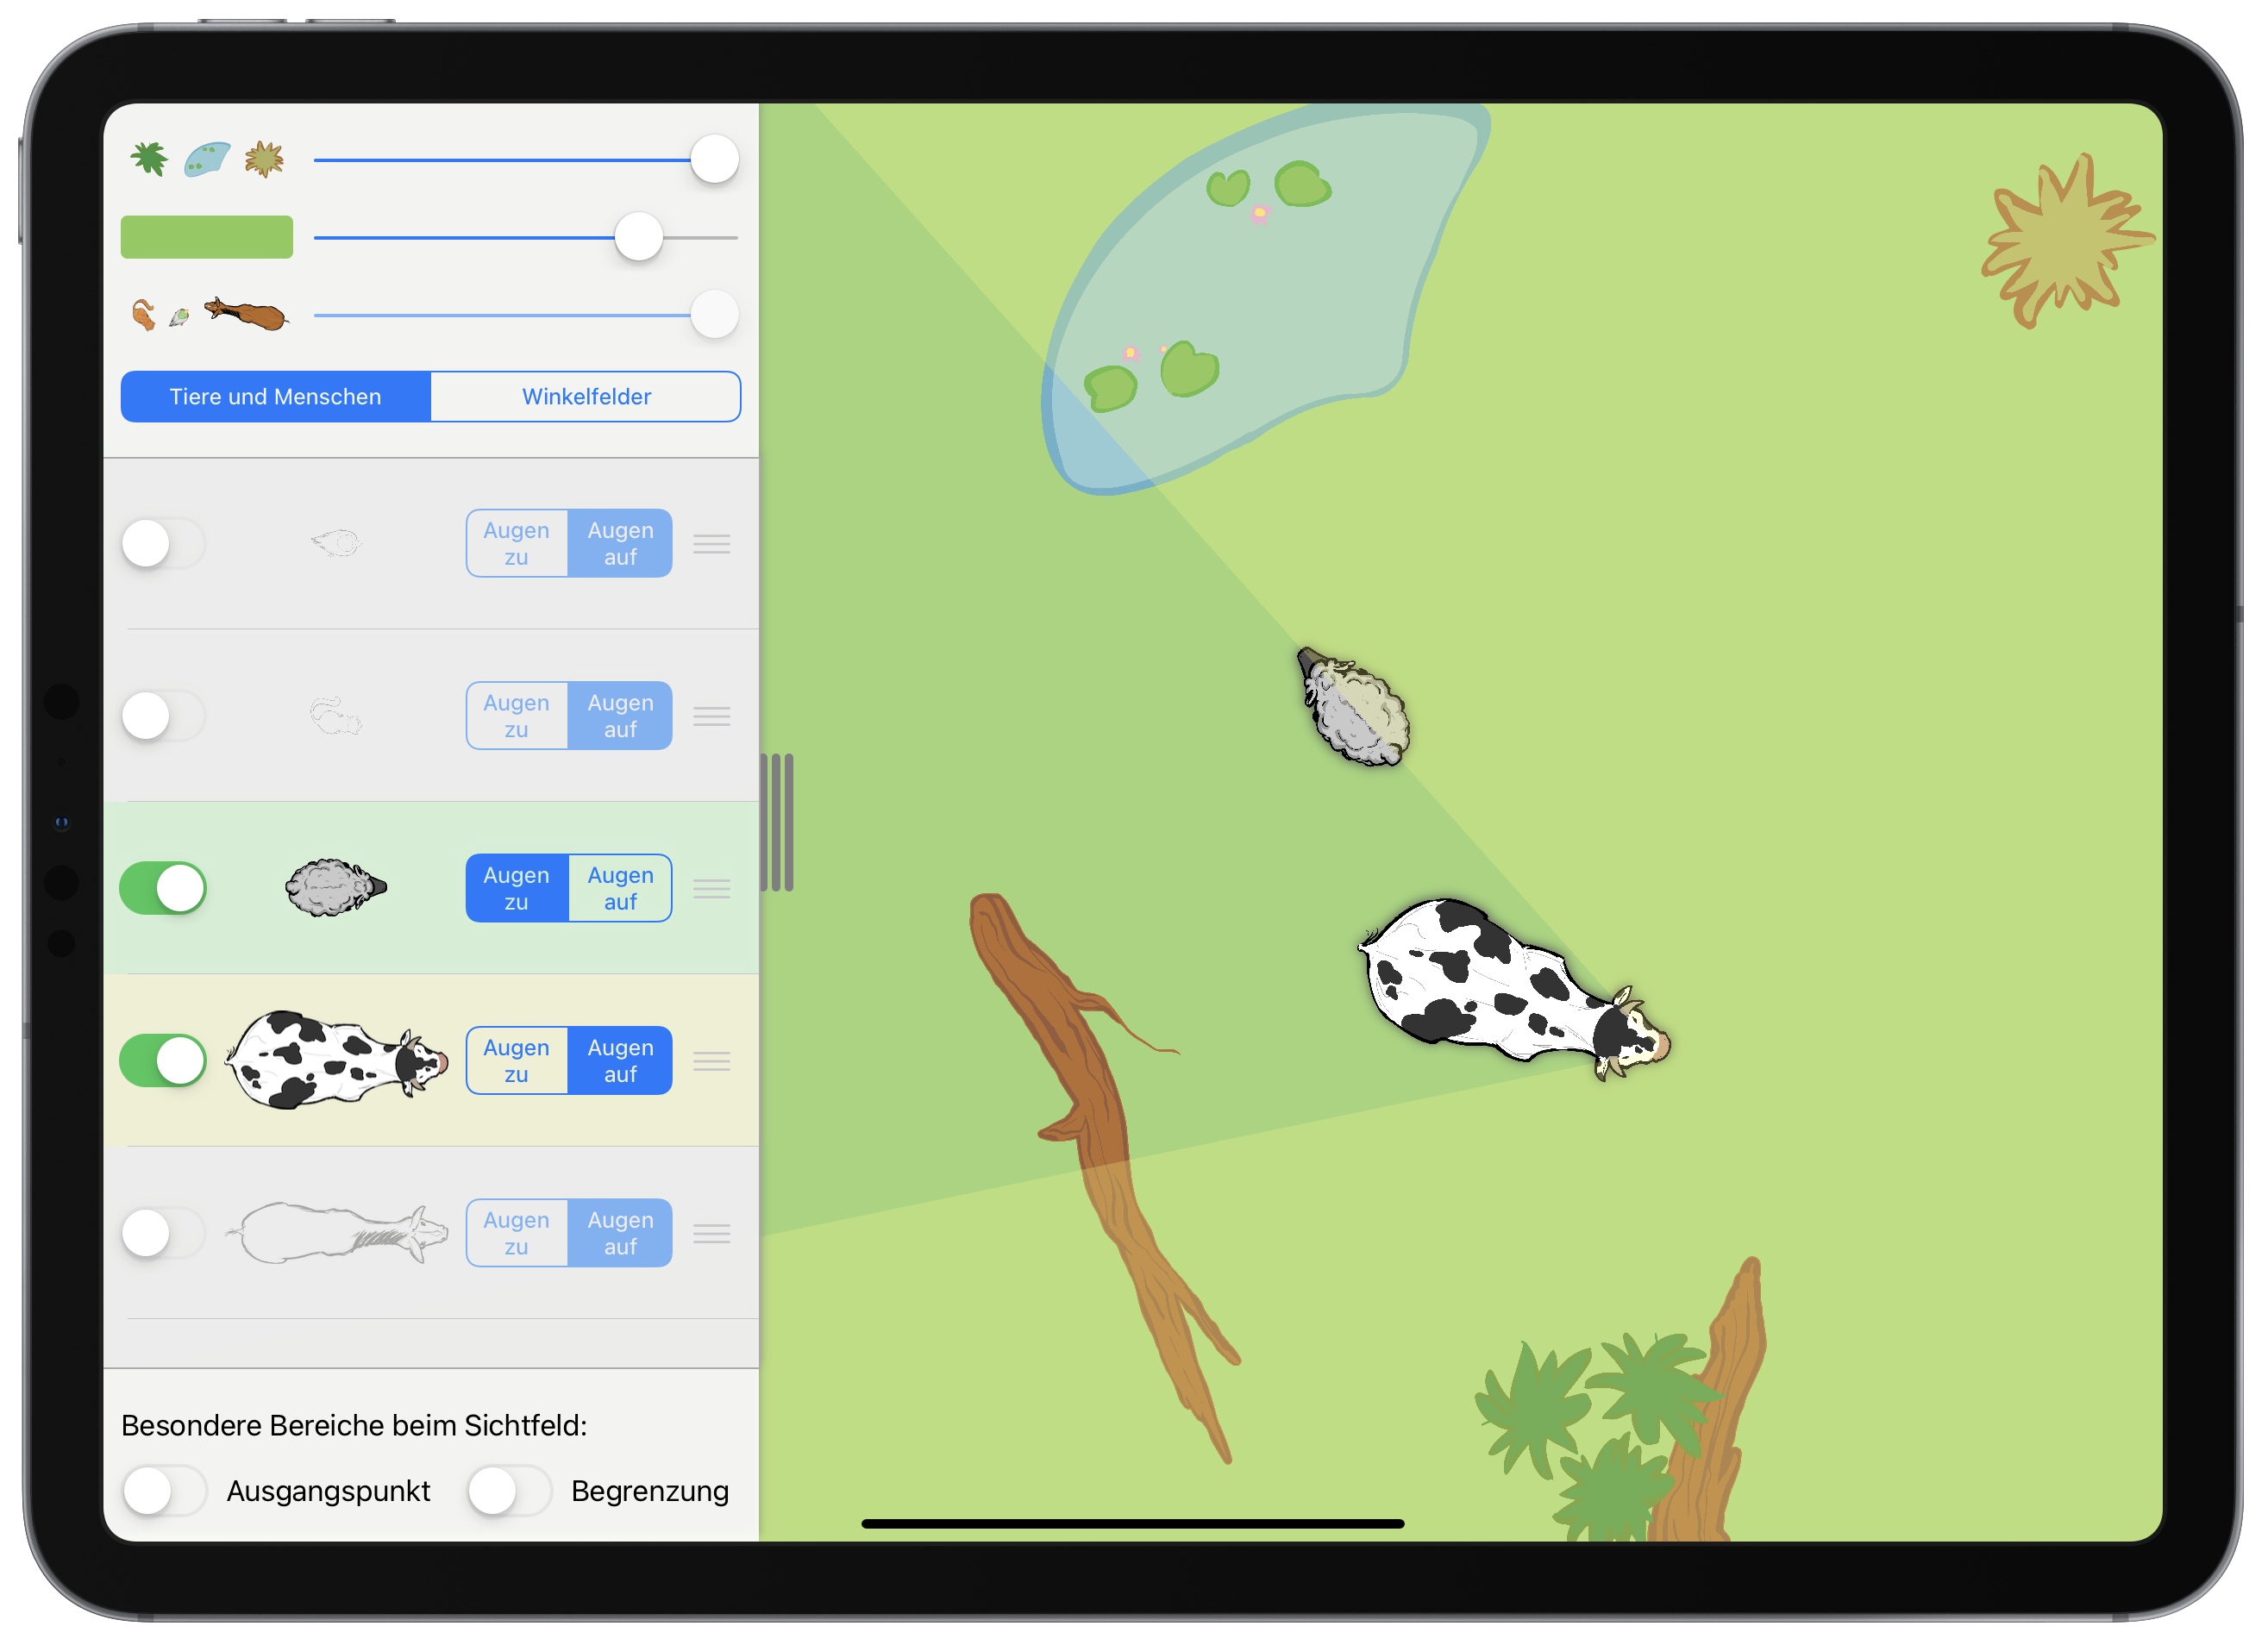
\includegraphics[width=0.5\linewidth]{pictures/1-Winkelfarm} 

}

\caption{Lernhandlung in der App \emph{Winkel-Farm} (\citeproc{ref-Etzold:2019}{Etzold, 2019a})}\label{fig:HandlungSchaf}
\end{figure}

Welche Schritte für die Ausbildung von Lernhandlungen notwendig sind, wird im nächsten Kapitel dargestellt.
Zu betonen ist, dass die Lernhandlungen zwar einerseits notwendig sind, um sich einem Lerngegenstand zu nähern, also die \textbf{Handlungen als \emph{Lernmittel}} aufgefasst werden können. Andererseits müssen die Lernhandlungen jedoch auch erst einmal ausgeprägt werden, also auch die \textbf{Handlungen als \emph{Lerngegenstand}} selbst aufgefasst werden (was wiederum nur am konkreten mathematischen Unterrichtsthema realisiert werden kann). Diese Sichtweise sollte Sie als Lehrkraft dafür sensibilisieren, dass Sie nicht per se davon ausgehen können, dass Ihre Schülerinnen und Schüler über entsprechende Handlungen verfügen, um neue mathematische Themen zu erlernen, sondern an diesen Themen die Handlungen erarbeitet und mit den Handlungen die Mathematik erarbeitet wird. Auch hier kann wieder von der zunächst gemeinschaftlichen Handlungsausführung (in der Klassensituation und mit Unterstützung von Personen, die über das anzueignende Wissen verfügen) zur individuellen Handlungsausführung (und damit persönlichen Aneignung des Lerngegenstands) übergegangen werden.

\section{Motivierung und Zielbildung}\label{motivierung-und-zielbildung}

Die obigen Überlegungen zeigen, dass die \textbf{Motivierung und Zielbildung} bedeutsame Bestandteile eines Lernprozesses sind, sich also in der Gestaltung konkreter Unterrichtssituationen widerspiegeln müssen -- durch entsprechende Phasen innerhalb einer Unterrichtsstunde. Erst wenn Motive und Ziele ausgeprägt sind, kann es in weiteren Unterrichtsphasen zur \textbf{Ausbildung der Lernhandlungen} kommen.

\subsection{Zone der nächsten Entwicklung}\label{zone-der-nuxe4chsten-entwicklung}

Die Schülerinnen und Schüler müssen zunächst in die Lage versetzt werden, sich mit dem Lerngegenstand auseinandersetzen zu \emph{wollen}. Hierzu ist es (aus lernpsychologischer Sicht) hilfreich, die Anforderungssituation in der \textbf{Zone der nächsten Entwicklung} der Schülerinnen und Schüler zu präsentieren. Dabei handelt es sich um eine Problemsituation, Aufgabe oder Fragestellung, die die Schülerinnen und Schüler zwar mithilfe ihrer bisherigen Kenntnisse, Fähigkeiten und Fertigkeiten \textbf{verstehen und nachvollziehen} können, zu ihrer Lösung sie jedoch noch \textbf{nicht selbstständig} (aber mit Unterstützung wissender Personen) in der Lage sind. Somit wird eine Motivation geschaffen, sich mit der Thematik tiefer auseinanderzusetzen. Es ist durchaus möglich, an dieser Stelle auch schon erste Lösungsversuche zu unternehmen. Daran ist besonders gut zu erkennen, »was wir nicht wissen bzw. können, um die Anforderung zu bewältigen« (\citeproc{ref-Lompscher1996}{Lompscher, 1996, S. 4}).

Dem kann die \textbf{Zone der aktuellen Leistung} gegenübergestellt werden, also Probleme bzw. Aufgaben, die die Schülerinnen und Schüler bereits selbstständig lösen können. Würde jedoch jede Anforderungssituation in der Zone der aktuellen Leistung liegen, wäre langfristig kein Lernzuwachs möglich (und insbesondere könnte sich keine Motivation zum Lernen einstellen).

Ein bestimmtes Niveau eines Individuums ist dadurch gekennzeichnet, dass es zu bestimmten Dingen selbstständig in der Lage ist, zu anderen jedoch noch nicht. Der Übergang zum nächst höheren Niveau erfolgt, indem die soeben noch nicht selbstständig lösbaren Problemstellungen (in der Zone der nächsten Entwicklung) zu selbstständig lösbaren Problemstellungen (in der Zone der aktuellen Leistung) werden. Ein solcher Niveauübergang erfolgt Lompscher (\citeproc{ref-Lompscher1985b}{1985, S. 26}) zufolge durch »pädagogische Führung«. Diese etwas sperrige Bezeichnung drückt jedoch nichts anderes aus, als dass die Lehrkraft für die Gestaltung des Lernprozesses verantwortlich ist, damit die Schülerinnen und Schüler den entsprechenden Niveauübergang vollführen können.



\begin{figure}

{\centering 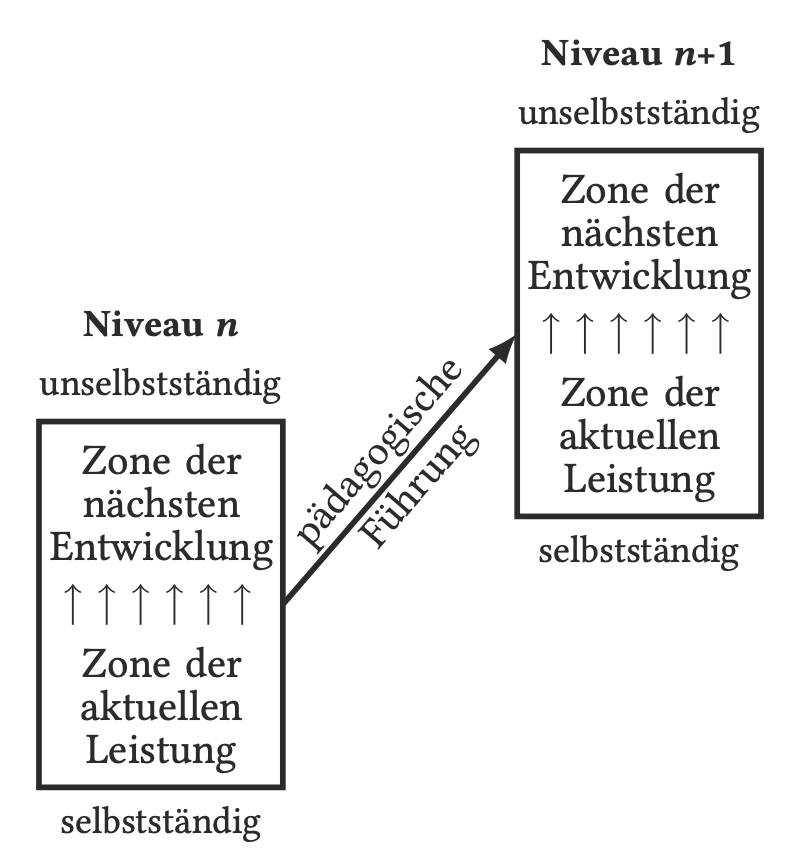
\includegraphics[width=0.5\linewidth]{pictures/5-ZdnE} 

}

\caption{Zone der nächsten Entwicklung (nach \citeproc{ref-Lompscher1985b}{Lompscher, 1985, S. 26})}\label{fig:ZdnE}
\end{figure}

\begin{quote}
Beim Winkelfeld wurden den Schülerinnen und Schülern Fotos verschiedener Tiere präsentiert, die teils ihre Augen an der Seite des Kopfes und teils nach vorn gerichtet hatten. Es wurde besprochen, was diese Tiere unterscheidet (Flucht- und Jagdtiere) und welche Bedeutung die Lage der Augen hierfür haben kann. Diese Situation ist für die Schülerinnen und Schüler nachvollziehbar, aber sie können noch nicht selbstständig beschreiben, welcher geometrische Zusammenhang zwischen der Position der Augen und der Lebensweise der Tiere besteht.
\end{quote}

\subsection{Lernzielbildung}\label{lernzielbildung}

Aus dem Motiv heraus, sich mit einem konkreten Lerngegenstand zu beschäftigen, erfolgt eine geistige Vorwegnahne, was das \emph{Ergebnis} der Lerntätigkeit ist. Darunter sind neue »Handlungen, Verhaltensweisen, Bedeutungen, Werte, Normen, Begriffe, Gesetzmäßigkeiten usw. in Form von Kenntnissen, Fähigkeiten, Einstellungen und anderen psychischen Eigenschaften« zu verstehen (\citeproc{ref-Lompscher1985b}{Lompscher, 1985, S. 40}). Solche (psychischen) Ergebnisse unterscheiden sich damit von (äußeren) \emph{Produkten} wie »Zeichnungen, schriftliche Arbeiten, Materialsammlungen, Werkstücke, mündliche Aussagen u.~a.« (\citeproc{ref-Lompscher1985b}{Lompscher, 1985, S. 40}).

Die Orientierung darauf, eines der \emph{Ergebnisse} zu erzielen, entspricht demnach dem \textbf{Lernziel}. Hier ist zu beachten, dass das \emph{Lernziel} nicht zu verwechseln ist mit dem von der Lehrkraft erwünschten \emph{Lehrziel}.\footnote{Erst recht nicht zu verwechseln ist der Begriff mit den »Lernzielen« außerhalb der Tätigkeitstheorie, die bspw. bei einer Unterrichtsplanung angegeben werden. Letztere entsprechen eher den Lehrzielen und können auch -- um Verwechslungen zu vermeiden -- als \emph{Kompetenzziele} bezeichnet werden, da sie Kompetenzen beschreiben, die am Ende der entsprechenden Unterrichtsstunde ausgebildet worden sein sollen.} Lernziele werden individuell von den Schülerinnen und Schülern ausgeprägt. Sie haben jedoch als Lehrkraft die Aufgabe, eine solche Lernzielbildung zu unterstützen und idealerweise auch zu lenken, so dass die Schülerinnen und Schüler für den Lerngegenstand adäquate Lernziele bilden. Der Grad der \textbf{Bewusstheit, Allgemeinheit und Differenziertheit} des Lernziels bestimmt dabei letztlich auch, in welcher Qualität die darauf basierenden Lernhandlungen ausgeprägt werden (vgl. \citeproc{ref-Lompscher1985b}{Lompscher, 1985, S. 43}). Möchte ein Kind einfach nur die Lösung der Aufgabe \(17+8\) ermitteln (Produktorientierung), so wird es nicht so qualitativ hochwertig und nachhaltig lernen können, als wenn es das Ziel verfolgt, grundsätzlich Additionsaufgaben mit Zehnerübergang lösen zu können (Ergebnisorientierung).

Es bietet sich eine \textbf{explizite Verbalisierung und auch das Festhalten von Lernzielen} (z.~B. an der Tafel) an, um während des Lernprozesses darauf zurückgreifen und seinen eigenen Handlungsfortschritt permanent mit den Zielen abgleichen zu können.

\begin{quote}
Anknüpfend an die Präsentation der Tierbilder zu Winkelfeldern wurde, von der Lehrkraft durch ein Lehrer-Schüler-Gespräch initiiert, als Lernziel formuliert: »Wir wollen Sichfelder von Tieren beschreiben und miteinander vergleichen« (vgl. \citeproc{ref-Etzold:2019Praxis4}{Etzold, 2019b, S. 6}). Diese Zielformulierung enthält bewusst keine mathematischen Fachbegriffe des neuen Lerngegenstandes, da diese zum entsprechenden Zeitpunkt ja noch gar nicht erarbeitet worden sind.
\end{quote}

Wie das Beispiel schon zeigt, müssen Motivierung und Zielbildung nicht als getrennte Unterrichtsphasen strukturiert werden. Relevant ist jedoch, \emph{dass} sie stattfinden und einen bedeutsamen Raum im Unterricht einnehmen. Ein Unterrichtsbeginn mit »Wir beschäftigen uns heute mit \ldots« liefert eben i.~d.~R. keine Motivation und löst in den Schülerinnen und Schülern keine Lernzielbildung aus, was für den weiteren Lernprozess extrem hinderlich ist. Auch zeigt sich hier wieder die \textbf{Bedeutung der Lehrkaft}: Sie ist diejenige, die die Schülerinnen und Schüler in die Lage versetzen kann, sich dem Lerngegenstand zu nähern. Das heißt insbesondere auch, dass ein \emph{Ostereiersuchen} vermieden werden muss (bei dem die Schülerinnen und Schüler z.~B. so lange raten, um was es denn heute gehen könnte, bis sie die richtige Antwort gefunden haben), sondern die Lehrkraft \emph{instruiert} (persönlich oder durch geeignete Aufgabenstellungen) unter Berücksichtigung der individuellen Voraussetzungen der Schülerinnen und Schüler einen ersten Zugang zum Lerngegenstand. Damit ist die Lehrkraft ein Vertreter des gesellschaftlichen Wissens und Könnens, das sich die Schülerinnen und Schüler als Kenntnisse, Fähigkeiten und Fertigkeiten aneignen werden.

\section{Orientierungsbildung}\label{orientierungsbildung}

Mit der Erfassung einer Anforderungssituation geht ad hoc eine Orientierung der Schülerinnen und Schüler bezüglich der möglichen Bearbeitung einher. Dabei wird in drei Qualitäten von \textbf{\emph{Orientierungsgrundlagen}} unterschieden (als Zitate gekennzeichnete Formulierungen sind entnommen aus \citeproc{ref-Feldt-Caesar2017}{Feldt-Caesar, 2017, 83~ff.}):

\begin{itemize}
\item
  \textbf{Probierorientierung:} Die Schülerinnen und Schüler verfügen noch nicht über für die Aufgabenbewältigung nötigen Kenntnisse, Fähigkeiten oder Fertigkeiten. Stattdessen gehen sie nach Versuch und Irrtum vor. Dabei fehlt ihnen »häufig die Einsicht, warum eine bestimmte Handlung zum Erfolg geführt hat, eine andere jedoch nicht. {[}\ldots{]} Aufgrund der mangelnden Einsicht in die wirklichen Bedingungen der Handlungen ist eine erfolgreiche Handlung nicht notwendigerweise reproduzierbar.« Dies führt dazu, dass erfolgreiche Handlungen kaum auf veränderte Situationen übertragen werden können. Eine derartige Orientierung ist also höchstens »in Aneignungsprozessen zu einem Explorieren des neuen Inhaltsbereichs« wünschenswert, darüber hinaus jedoch sollten höhere Orientierungsgrundlagen angestrebt werden.
\item
  \textbf{Musterorientierung:} Die Schülerinnen und Schüler gehen nun nicht mehr nach Versuch und Irrtum vor, sondern orientieren sich an bereits erfolgreich durchgeführten Handlungen in ähnlichen Anforderungssituationen -- die sozusagen als Muster dienen.
  »Dieser Orientierungstyp ist nur dann erfolgreich, wenn die gegebene Anforderungssituation dem erlernten Muster ähnlich genug ist, um eine Passung zu ermöglichen. Tragfähig ist ein Muster nur dann, wenn seine Handlungsbedingungen genau gekannt und stets geprüft werden.«
  Es handelt sich also zwar um eine vollständige Orientierungsgrundlage, jedoch ist eine Transferierbarkeit nicht immer gegeben. Auch kann die »fälschliche Erkennung eines Musters in einer gegebenen Anforderungssituation« zu einer fehlerhaften Übertragung führen.
\item
  \textbf{Feldorientierung:} Die Schülerinnen und Schüler sind nun »nicht an eine konkrete Anforderungssituation gebunden, sondern beziehen sich vielmehr auf ganze Anforderungsklassen. Durch das Erkennen der Passung einer solchen Anforderungsklasse kann sich der Lernende für konkrete Situationen selbst eine Orientierung schaffen. Er verfügt über einen gewissen Überblick über die Situation und ist in der Lage zu differenzieren, welche Stoffelemente und welche seiner Kenntnisse, Fähigkeiten und Fertigkeiten ihm bei der Bewältigung der Anforderung weiterhelfen können und welche nicht.« Aufgrund des hohen Maßes an Übertragbarkeit ist eine Feldorientierung insbesondere für Kenntnisse, Fähigkeiten und Fertigkeiten, die in den Bereich von Mindeststandards fallen, von Bedeutung: »Feldorientierung gilt als erstrebenswert für solche Lerninhalte, die für erfolgreiches Weiterlernen unabdingbar sind.« (\citeproc{ref-Richter2016}{Richter \& Bruder, 2016, S. 195})
\end{itemize}

Auch wenn eine Feldorientierung erstrebenswert ist, wird diese vermutlich nicht immer von allen Schülerinnen und Schülern erreicht werden können. Diesen Schülerinnen und Schülern sollten Sie jedoch dahingehend Unterstützung bieten, zumindest eine Musterorientierung zu erlangen. Hierzu gehört auch, das \emph{Erfüllen eines Musters} explizit zu machen, also bei gegebenen Aufgabenstellungen zu untersuchen, inwieweit diese einem bereits bekannten Muster entsprechen und wie sie damit lösbar sind. Ebenfalls hilfreich, und auch den Übergang zur Feldorientierung stützend, sind \textbf{Orientierungshilfen}, also Verbalisierungen oder Repräsentationen zum Lerngegenstand, die beim Finden geeigneter Lernhandlungen unterstützen. Solche Orientierungshilfen sollten gemeinsam aus der ersten Beschäftigung mit dem Lerngegenstand herausgearbeitet und in den Umgang mit ihnen eingeführt werden, damit sie sinnvoll in den Lernprozess integriert werden können.

Beispiele für Orientierungshilfen bei der Aneignung von Begriffen, Zusammenhängen und Verfahren finden sich in den nächsten Kapiteln.

\begin{quote}
Die App Winkel-Farm unterstützt die Aneignung des Begriffs »Schenkel« eines Winkel mit dessen Strahl-Eigenschaft, indem sich die Bestandteile des Winkelfeldes ein- und ausblenden lassen sowie vom \emph{Tiermodus} in den \emph{Winkelfeldmodus} gewechselt werden kann und damit das Wesen des Begriffs hervorgehoben werden kann.
\end{quote}

\section{Bezüge zur Stoffdidaktik}\label{bezuege-zur-stoffdidaktik}

\begin{itemize}
\item
  Der \textbf{Lerngegenstand} selbst als Ausschnitt des gesellschaftlichen Wissens und Könnens entspricht einem der Mathematik entstammenden \textcolor{formalColor}{**Begriff**, **Zusammenhang** oder **Verfahren**} bzw. einem Ausschnitt \textcolor{formalColor}{**metamathematischen Wissens**}. Er hat daher eine gesellschaftliche und historische Bedeutung, die es im Unterricht zu transportieren gilt.
\item
  Für die \textbf{Motivierung und Zielbildung} sollte ein \textcolor{concreteColor}{**sinnstiftender Kontext**} herangezogen werden, der in besonderer Weise charakteristisch für den zu erlernenden Lerngegenstand ist. Die \textcolor{concreteColor}{**Kernidee in der Vorschauperspektive**} unterstützt bei der Zielbildung, um das Wesen des neuen Lerngegenstands im Vorfeld deutlich machen zu können und die erwünschten Handlungsergebnisse im Blick zu haben. Es ist durchaus möglich, dass die explizite Lernzielformulierung in Form der \textcolor{concreteColor}{**Kernfragen**} erfolgt. Auch das \textcolor{semanticColor}{**Explizitmachen fundamentaler Ideen**} kann die Einordnung des neuen Lerngegenstands unterstützen.\footnote{Dies ist eine Adaption eines bei Reitz-Koncebovski et al. (\citeproc{ref-Reitz-Koncebovski2018}{2018, S. 182}) dargestellten Gestaltprinzips fachwissenschaftlicher Lehrveranstaltungen in der Lehramtsausbildung.}
\end{itemize}

Für die Unterrichtgestaltung wurde bisher verschwiegen, dass die Lernhandlungen selbstverständlich auf Vorkenntnisse und -fertigkeiten aufbauen und dieser bedürfen. Es ist daher unerlässlich, das für die neu zu erwerbenden Lernhandlungen benötigte \textbf{Ausgangsniveau zu sichern} (was dann die \emph{Zone der aktuellen Leistung} charakterisiert). Dies kann in \textbf{Wiederholungsphasen} zum aktuell benötigten Stoff erfolgen, dauerhaft und langfristig auch in (unbenoteten) \textbf{täglichen Übungen / vermischten Kopfübungen} zum »Wachhalten von Basiswissen« (siehe auch \citeproc{ref-Bruder2008b}{Bruder, 2008}).

\section{Zum Nachbereiten}\label{taetigkeitstheorie-nachbereitung}

Lösen sie folgende Aufgaben am Beispiel des Lerngegenstands \emph{Vierecksarten}.

\begin{enumerate}
\def\labelenumi{\arabic{enumi}.}
\item
  Formulieren Sie eine Anforderungssituation in der Zone der nächsten Entwicklung und stellen Sie dar, inwieweit diese zwar verstanden und nachvollzogen, aber noch nicht selbstständig gelöst werden kann.
\item
  Geben Sie mögliche Lernziele für den Lerngegenstand an.
\item
  Entwerfen Sie eine Orientierungshilfe zum Identifizieren von Vierecksarten.
\end{enumerate}

\chapter{Lernhandlungen ausbilden}\label{lernhandlungen-ausbilden}

\begin{quote}
\textbf{Ziele}

\begin{itemize}
\tightlist
\item
  Sie können typische Unterrichtssituationen im Mathematikunterricht benennen, beschreiben und lernpsychologisch begründen.
\item
  Ihnen ist die Bedeutsamkeit von Identifizierungs- und Realisierungshandlungen in der Stoffvermittlung bewusst.
\item
  Sie kennen eine Möglichkeit, wie geistige Handlungen schrittweise ausgebildet werden können.
\end{itemize}

\textbf{Material}

\begin{itemize}
\tightlist
\item
  Folien zum Kapitel 6 (\href{files/Stoffdidaktik2024-06-LernhandlungenAusbilden.pdf}{pdf}, \href{files/Stoffdidaktik2024-06-LernhandlungenAusbilden.key}{Keynote})
\end{itemize}
\end{quote}

\section{Aneignung von Lerngegenständen}\label{aneignung-von-lerngegenstaenden}

\subsection{Vermittelnde Werkzeuge}\label{vermittelnde-werkzeuge}

Nach Wygotski (\citeproc{ref-Wygotski1985a}{1985}) erfolgt eine Interaktion eines Individuums mit einem Lerngegenstand niemals direkt, sondern geschieht stets über ein \textbf{vermittelndes Werkzeug}. Es kann sich dabei um \emph{echte} Werkzeuge (wie Maschinen, Geräte und andere Hilfsmittel handeln) oder um \emph{psychische} Werkzeuge handeln, also Gesten, die Sprache, Abbildungen und Skizzen oder ähnliches. Entscheidend ist, dass dieses vermittelnde »Ding« für das Individuum die Funktion eines Vermittlers erfüllt.

Durch die Nutzung eines geeigneten Werkzeugs ist das Individuum damit einerseits in der Lage, seine Kenntnisse, Fähigkeiten und Fertigkeiten zu \textbf{\emph{externalisieren}}, d.~h. das Werkzeug zielgerichtet so einzusetzen, dass auf den Lerngegenstand eingewirkt werden kann. Andererseits kann das Werkzeug auch dabei helfen, Eigenschaften des Lerngegenstands zu \textbf{\emph{internalisieren}}, indem die Werkzeugnutzung dazu führt, dass das Individuum Kenntnisse, Fähigkeiten und Fertigkeiten über den Lerngegenstand gewinnt. Um sich also einen Lerngegenstand \emph{anzueignen}, sind sowohl stets Externalisierungs- als auch Internalisierungsprozesse notwendig. Man kann auch sagen, dass \textbf{Aneignung als Einheit aus Externalisierung und Internalisierung} aufzufassen ist.

\begin{figure}

{\centering 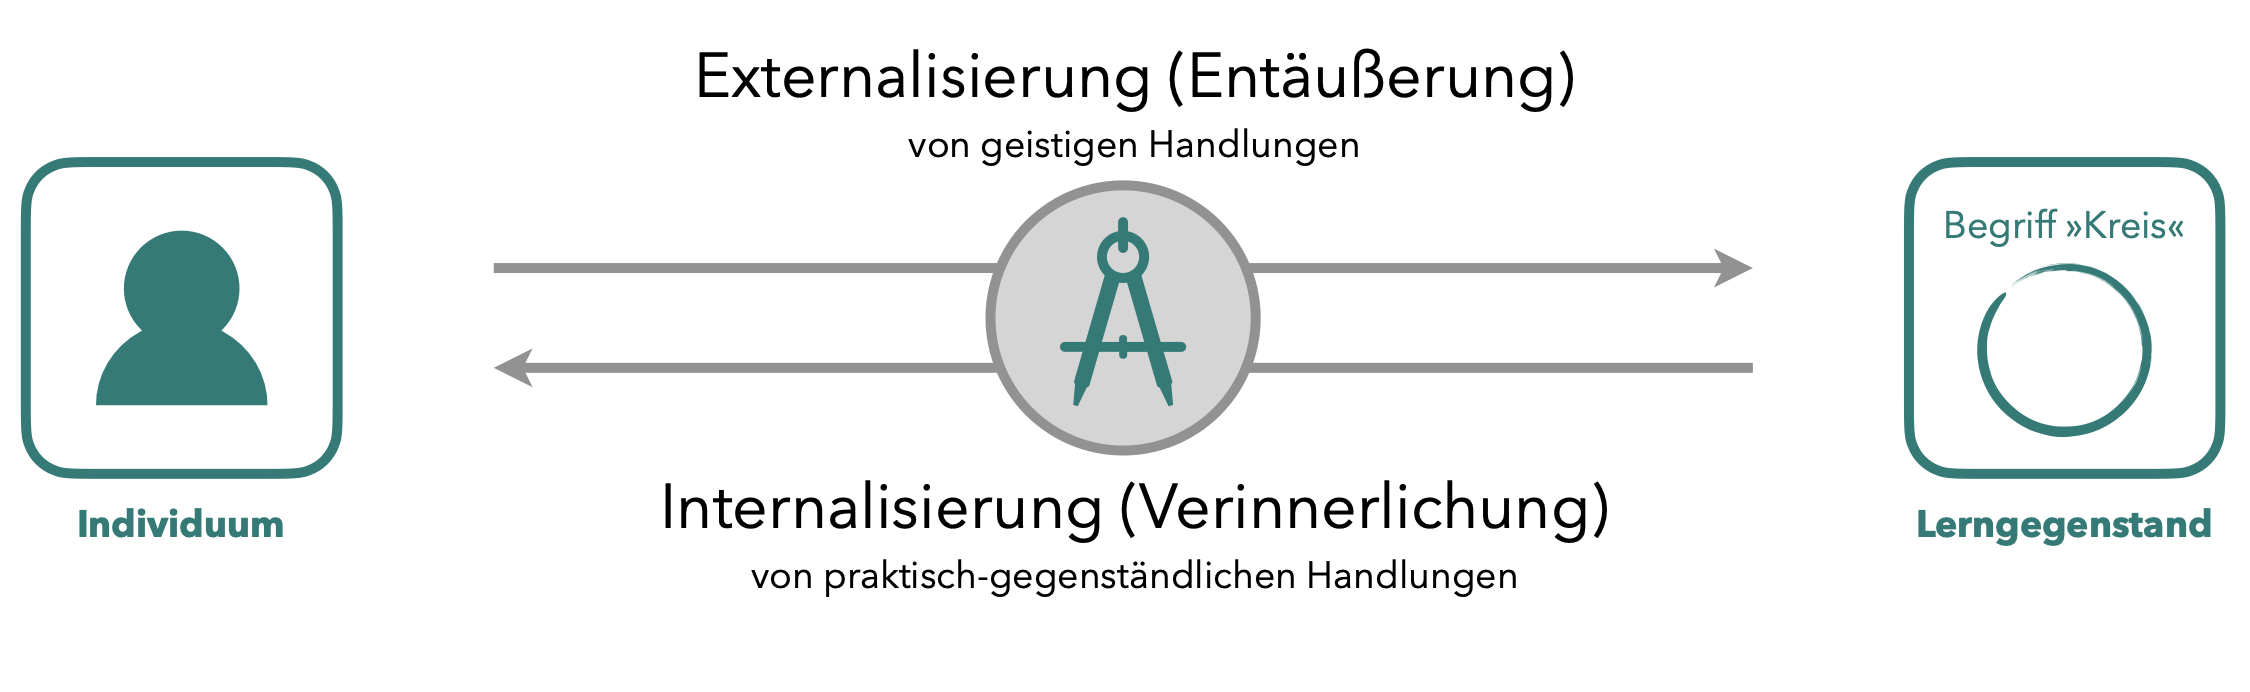
\includegraphics[width=0.75\linewidth]{pictures/6-Aneignung} 

}

\caption{Die Nutzung eines Zirkels zur Aneignung des Kreis-Begriffs}\label{fig:SubjektObjekt2}
\end{figure}

\subsection{Zur Rolle des Sprechens}\label{zur-rolle-des-sprechens}

Eine wichtige Rolle beim Aneignen spielt das \textbf{Sprechen über die durchgeführten Handlungen}. Dieses dient quasi als Bindeglied zwischen geistiger Handlung und praktisch-gegenständlicher Handlung, da es sowohl den Externalisierungsprozess unterstützt (das Geistige muss über das Sprechen externalisiert werden) als aus der Internalisierung dienlich ist (über das Sprechen wird das Praktisch-Gegenständliche psychisch verarbeitet). Damit unterstützt das Sprechen auch eine \textbf{schrittweise Abkehr vom externen Werkzeug} und damit eine geistige Durchdringung des betrachteten Lerngegenstands. Abbildung \ref{fig:GVverinnerlichen} zeigt eine entsprechende Schrittfolge zum Aufbau von Grundvorstellungen, wie sie Wartha \& Schulz (\citeproc{ref-Wartha2011}{2011, S. 11}) vorschlagen (wobei die dort verwendeten Farben nichts mit den hier im Skript genutzten Farben für die vier Ebenen zu tun haben).



\begin{figure}

{\centering 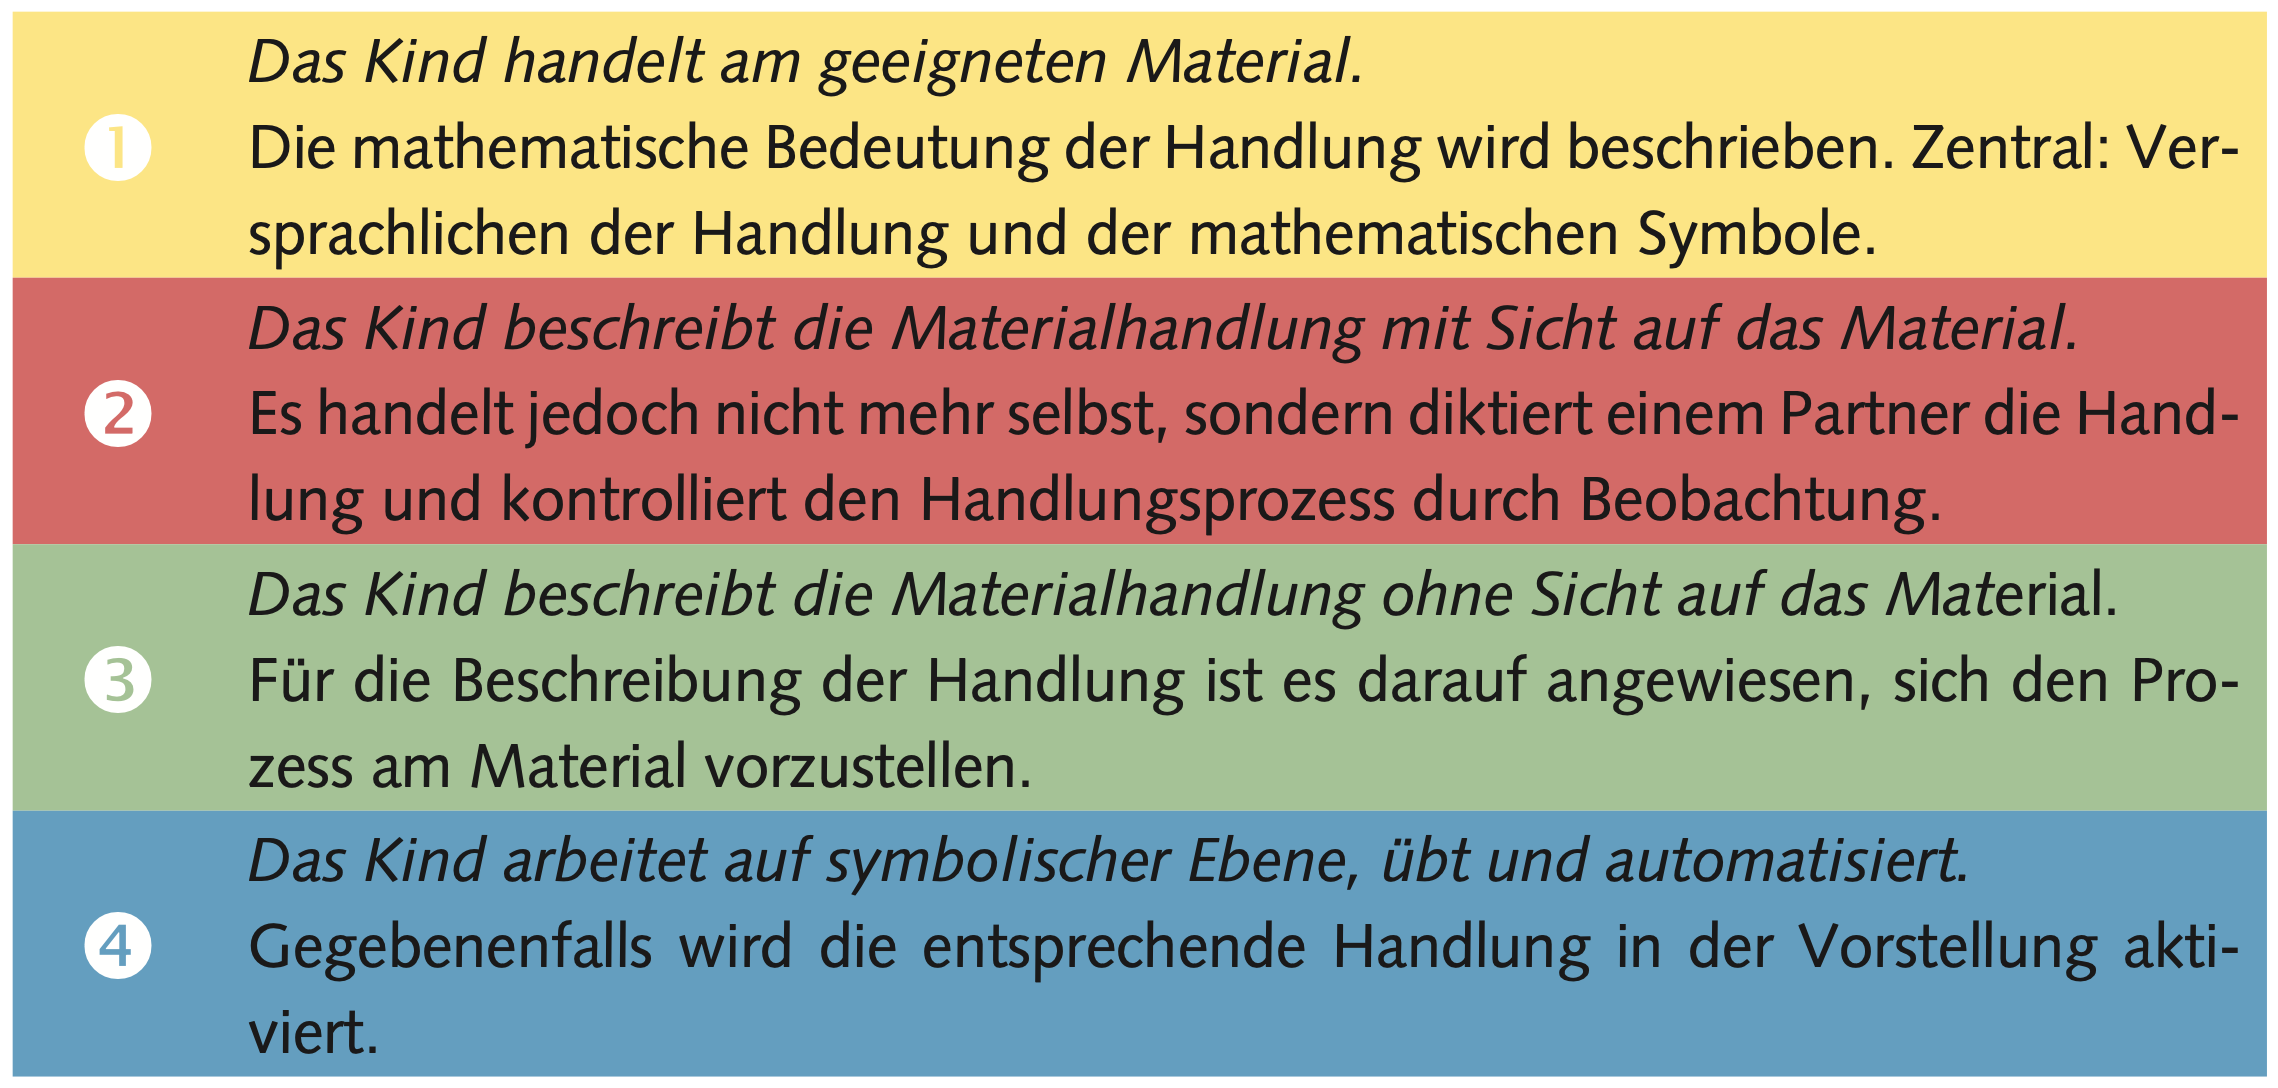
\includegraphics[width=0.75\linewidth]{pictures/6-GVverinnerlichen} 

}

\caption{Aufbau von Grundvorstellungen nach Wartha \& Schulz (\citeproc{ref-Wartha2011}{2011, S. 11})}\label{fig:GVverinnerlichen}
\end{figure}

In Abschnitt \ref{ausfuehren-und-verinnerlichen} wird diese Sichtweise noch einmal mit tätigkeitstheoretischen Theorien in Bezug gebracht.

\section{Typische Lernhandlungen}\label{typische-lernhandlungen}

Während Lern\emph{tätigkeit} allgemein auf die \emph{Aneignung} von Lerngegenständen fokussiert, kann diese nur über Lern\emph{handlungen} realisiert werden, also zielgerichtetes Vorgehen zur Auseinandersetzung mit dem Lerngegenstand.
Unabhängig von konkreten Lerngegenständen haben Bruder \& Brückner (\citeproc{ref-Bruder1989}{1989}) typische Lernhandlungen für den Mathematikunterricht strukturiert beschrieben (bereits kurz erwähnt in Abschnitt \ref{lerntaetigkeit-und-lernhandlung}), die hier noch einmal ausführlicher dargestellt und mit Beispielen belegt sind (Hervorhebungen im Original, auch dargestellt bei \citeproc{ref-Feldt-Caesar2017}{Feldt-Caesar, 2017, 87~ff.}):

\subsection{Elementare Aneignungshandlungen}\label{elementare-aneignungshandlungen}

\begin{itemize}
\item
  \textbf{Identifizieren:} »Vergleichen der aufgenommenen Informationen zu Teilen oder Eigenschaften eines Objektes mit den Merkmalen bestimmter aktualisierter Abbilder (Stoffelemente, Handlungsvorschriften \ldots) und Feststellung von Übereinstimmung oder Nichtübereinstimmung auf der Grundlage eines den jeweiligen Abbildungsmerkmalen entsprechenden \emph{Idealisierens} der gegebenen Objektsituation«

  \begin{quote}
  Beispiel: Erkennen, ob eine vorgegebene Figur ein Quadrat ist, nachdem der Begriff des Quadrats eingeführt wurde
  \end{quote}
\item
  \textbf{Realisieren:} »\emph{Transferieren}, Konkretisieren oder Spezialisieren eines vorgegebenen (bzw. identifizierten) Handlungsgegenstandes (Stoffelemente, Vorgehensstrategien \ldots) auf eine gegebene Objektsituation und \emph{Zusammenfügen} der so erzeugten Teile zu einem neuen Ganzen«

  \begin{quote}
  Beispiel: Angeben eines Beispiels für ein Zufallsexperiment, nachdem der Begriff des Zufallsexperiments eingeführt wurde
  \end{quote}
\end{itemize}

\subsection{Grundhandlungen}\label{grundhandlungen}

\begin{itemize}
\item
  \textbf{Erkennen:} »Ausgliedern wahrgenommener Informationen aus der Aufgabenstellung und Inbeziehungsetzen mit ausgegliederten bekannten (gespeicherten) Abbildern bzw. der neu zusammengefügten Abbilder, bis eine Übereinstimmung festgestellt wird«

  \begin{quote}
  Beispiel: Bestimmen der Nullstelle einer Funktion anhand des Funktionsgraphen. Hierbei muss zunächst anhand des Graphen identifiziert werden, dass die Stelle, an der der Graph die y-Achse schneidet, die Nullstelle ist. Anschließend muss der entsprechende Wert abgelesen werden.
  \end{quote}
\item
  \textbf{Beschreiben:} »Identifizieren und Realisieren einer dem gespeicherten (oder erzeugten) Abbild adäquaten umgangssprachlichen Formulierung oder Darstellung in mathematischer Terminologie und Symbolik und Entäußerung der Informationen auf sprachlicher oder materialisierter Ebene«

  \begin{quote}
  Beispiel: Vorgehen beschreiben, wie ein Kreis mit einem vorgegebenen Radius gezeichnet wird
  \end{quote}
\item
  \textbf{Verknüpfen:} »\emph{Transferieren} und \emph{Zusammensetzen} von Zusammenhängen (Sätzen, Verfahren) oder Vorgehensstrategien zu einem neuen Ganzen durch Ersetzungen in der Ausgangskonstellation von Zusammenhängen«

  \begin{quote}
  Beispiel: Finden einer Teilbarkeitsregel für 16, wenn die Teilbarkeitsregeln für 2, 4 und 8 bereits bekannt und begründet worden sind
  \end{quote}
\item
  \textbf{Anwenden:} »Feststellen der Übereinstimmung von den Bedingungen der Aufgabenstellung mit der Ausgangskonstellation der zu realisierenden gegebenen (oder erzeugten) Handlungsvorschrift (Identifizieren) und ggf. Herstellen einer solchen Übereinstimmung (Transferieren)«

  \begin{quote}
  Beispiel: Bestimmen der Lösungsmenge eines vorgegebenen linearen Gleichungssystems mithilfe des Additionsverfahrens.
  \end{quote}

  Mit \emph{Anwenden} in diesem Sinne ist nicht die Anwendung auf eine Realsituation gemeint.
\item
  \textbf{Begründen:} »a) Vergleichen eines vorgegebenen Sachverhalts mit gegebenen bzw. bekannten Normativen; b) Realisieren gegebener bzw. identifizierter elementarer Beweisverfahren«

  \begin{quote}
  Beispiel: Begründen, warum die Summe dreier aufeinanderfolgender natürlicher Zahlen durch 3 teilbar ist
  \end{quote}
\end{itemize}

\subsection{Komplexe Handlungen}\label{komplexe-handlungen}

\begin{itemize}
\item
  \textbf{Suchen:} »Ergebnis von Suchhandlungen sind zieltaugliche Mittel (Stoffelemente, Zuordnungen, Vorgehensstrategien) zur Lösung der gestellten Aufgabe -- gewonnen durch mehr oder weniger bewußte Anwendung von Suchstrategien«

  \begin{quote}
  Am Beispiel der Modellierungsaufgabe »Wie viele Luftballons passen in diesen Raum?«: Suchen des Lösungsansatzes, die Situation geometrisch zu modellieren
  \end{quote}
\item
  \textbf{Planen:} »Durch Anwenden von Vorgehensstrategien wird ein Arbeitsplan mit den erforderlichen Teilschritten zur Zielrealisierung entwickelt«

  \begin{quote}
  Am Beispiel der Modellierungsaufgabe »Wie viele Luftballons passen in diesen Raum?«: zunächst Modellieren des Raums als Quader, der Luftballons als Kugeln; dann Schätzen/Messen der Größen und Nutzen der Volumenformeln; weiterhin Inbeziehungsetzen der Volumina
  \end{quote}
\item
  \textbf{Ausführen:} »Abarbeiten eines Arbeitsplanes -- Handlungsvollzug auf der Grundalge der ausgebildeten Orientierungsgrundlage u.~a. als Berechnen, geometrisches Darstellen, Definieren, Darstellen eines Beweises«

  \begin{quote}
  Am Beispiel der Modellierungsaufgabe »Wie viele Luftballons passen in diesen Raum?«: Berechnen der entsprechenden Größen
  \end{quote}
\item
  \textbf{Kontrollieren:} »Feststellen der Zweckmäßigkeit und Exaktheit von Teilschritten des Aufgabenlösens und des Resultats (Handlungsprodukt!)«

  \begin{quote}
  Am Beispiel der Modellierungsaufgabe »Wie viele Luftballons passen in diesen Raum?«: Validieren des Ergebnisses; ggf. Entscheidung zu weiterem Durchgang des Modellierungskreislaufes
  \end{quote}
\end{itemize}

Diese Handlungen müssen nun je nach Lerngegenstand noch konkretisiert werden.

\section{Ausführen und Verinnerlichen}\label{ausfuehren-und-verinnerlichen}

Am neu zu erlernenden Lerngegenstand werden die Schülerinnen und Schüler nun \textbf{an die Ausführung geeigneter Lernhandlungen herangeführt}, was bspw. über ein Vorführen und Erklären durch die Lehrkraft erfolgen kann. Die Ausführung durch die Schülerinnen und Schüler darf jedoch nicht mit einem \emph{Nachahmen} verwechselt werden. Vielmehr erfolgen die Handlungen \textbf{einsichtig} und das \textbf{Lernziel verfolgend}, ggf. unter \textbf{Verwendung der Orientierungshilfen}. Je nach Vorkenntnissen können die Schülerinnen und Schüler auch, angeregt durch entsprechende Aufgabenstellungen, selbstständig die neuen Lernhandlungen durchführen, wobei nicht davon auszugehen ist, dass sie bereits über alle Voraussetzungen verfügen, die Lernhandlungen vollumfänglich zu nutzen (denn sonst wäre die zugehörige Anforderungssituation nicht in der Zone der nächsten Entwicklung gewesen).

Um die Lernhandlungen zu \emph{verinnerlichen} (genauer: um sie \emph{anzueignen}, was stets als Einheit aus Entäußerung und Verinnerlichung anzusehen ist -- vgl. Abschnitt \ref{aneignung-von-lerngegenstaenden}) schlägt Gal'perin eine \textbf{»etappenweise Interiorisierung«} vor (vgl. \citeproc{ref-Lompscher1985a}{Lompscher, 1983, 66~f.}):

\begin{itemize}
\item
  \textbf{Etappe der materiellen bzw. materialisierten Handlung}: Die Handlungen werden mit konkretem Material (z.~B. Arbeitsmitteln) oder anderen schriftlich vorliegenden Orientierungshilfen zum Lerngegenstand durchgeführt.
\item
  \textbf{Etappe der sprachlichen Handlung}: Die Handlungen werden ohne oder nur mit geringer Zuhilfenahme des Materials durchgeführt und dabei durch äußeres (oder inneres) Sprechen beschrieben. Dabei wird i.~d.~R. Bezug auf die vorherigen Handlungen genommen.
\item
  \textbf{Etappe der geistigen Handlung}: Die Handlungen werden nun rein kognitiv durchgeführt und bedürfen weder des Materials noch der Sprache.
\end{itemize}

Diese Etappen führen letztlich dazu, die Lernhandlungen (und damit auch den Lerngegenstand, an dem diese Handlungen durchgeführt werden) psychisch abbilden zu können, was zur »Verallgemeinerung, Verkürzung und Beherrschung« der Handlungen führt (\citeproc{ref-Steinhofel1988}{Steinhöfel et al., 1988, S. 19}). Abbildung \ref{fig:Etappen} zeigt hierzu einige Realisierungsmöglichkeiten für den Mathematikunterricht.



\begin{figure}

{\centering 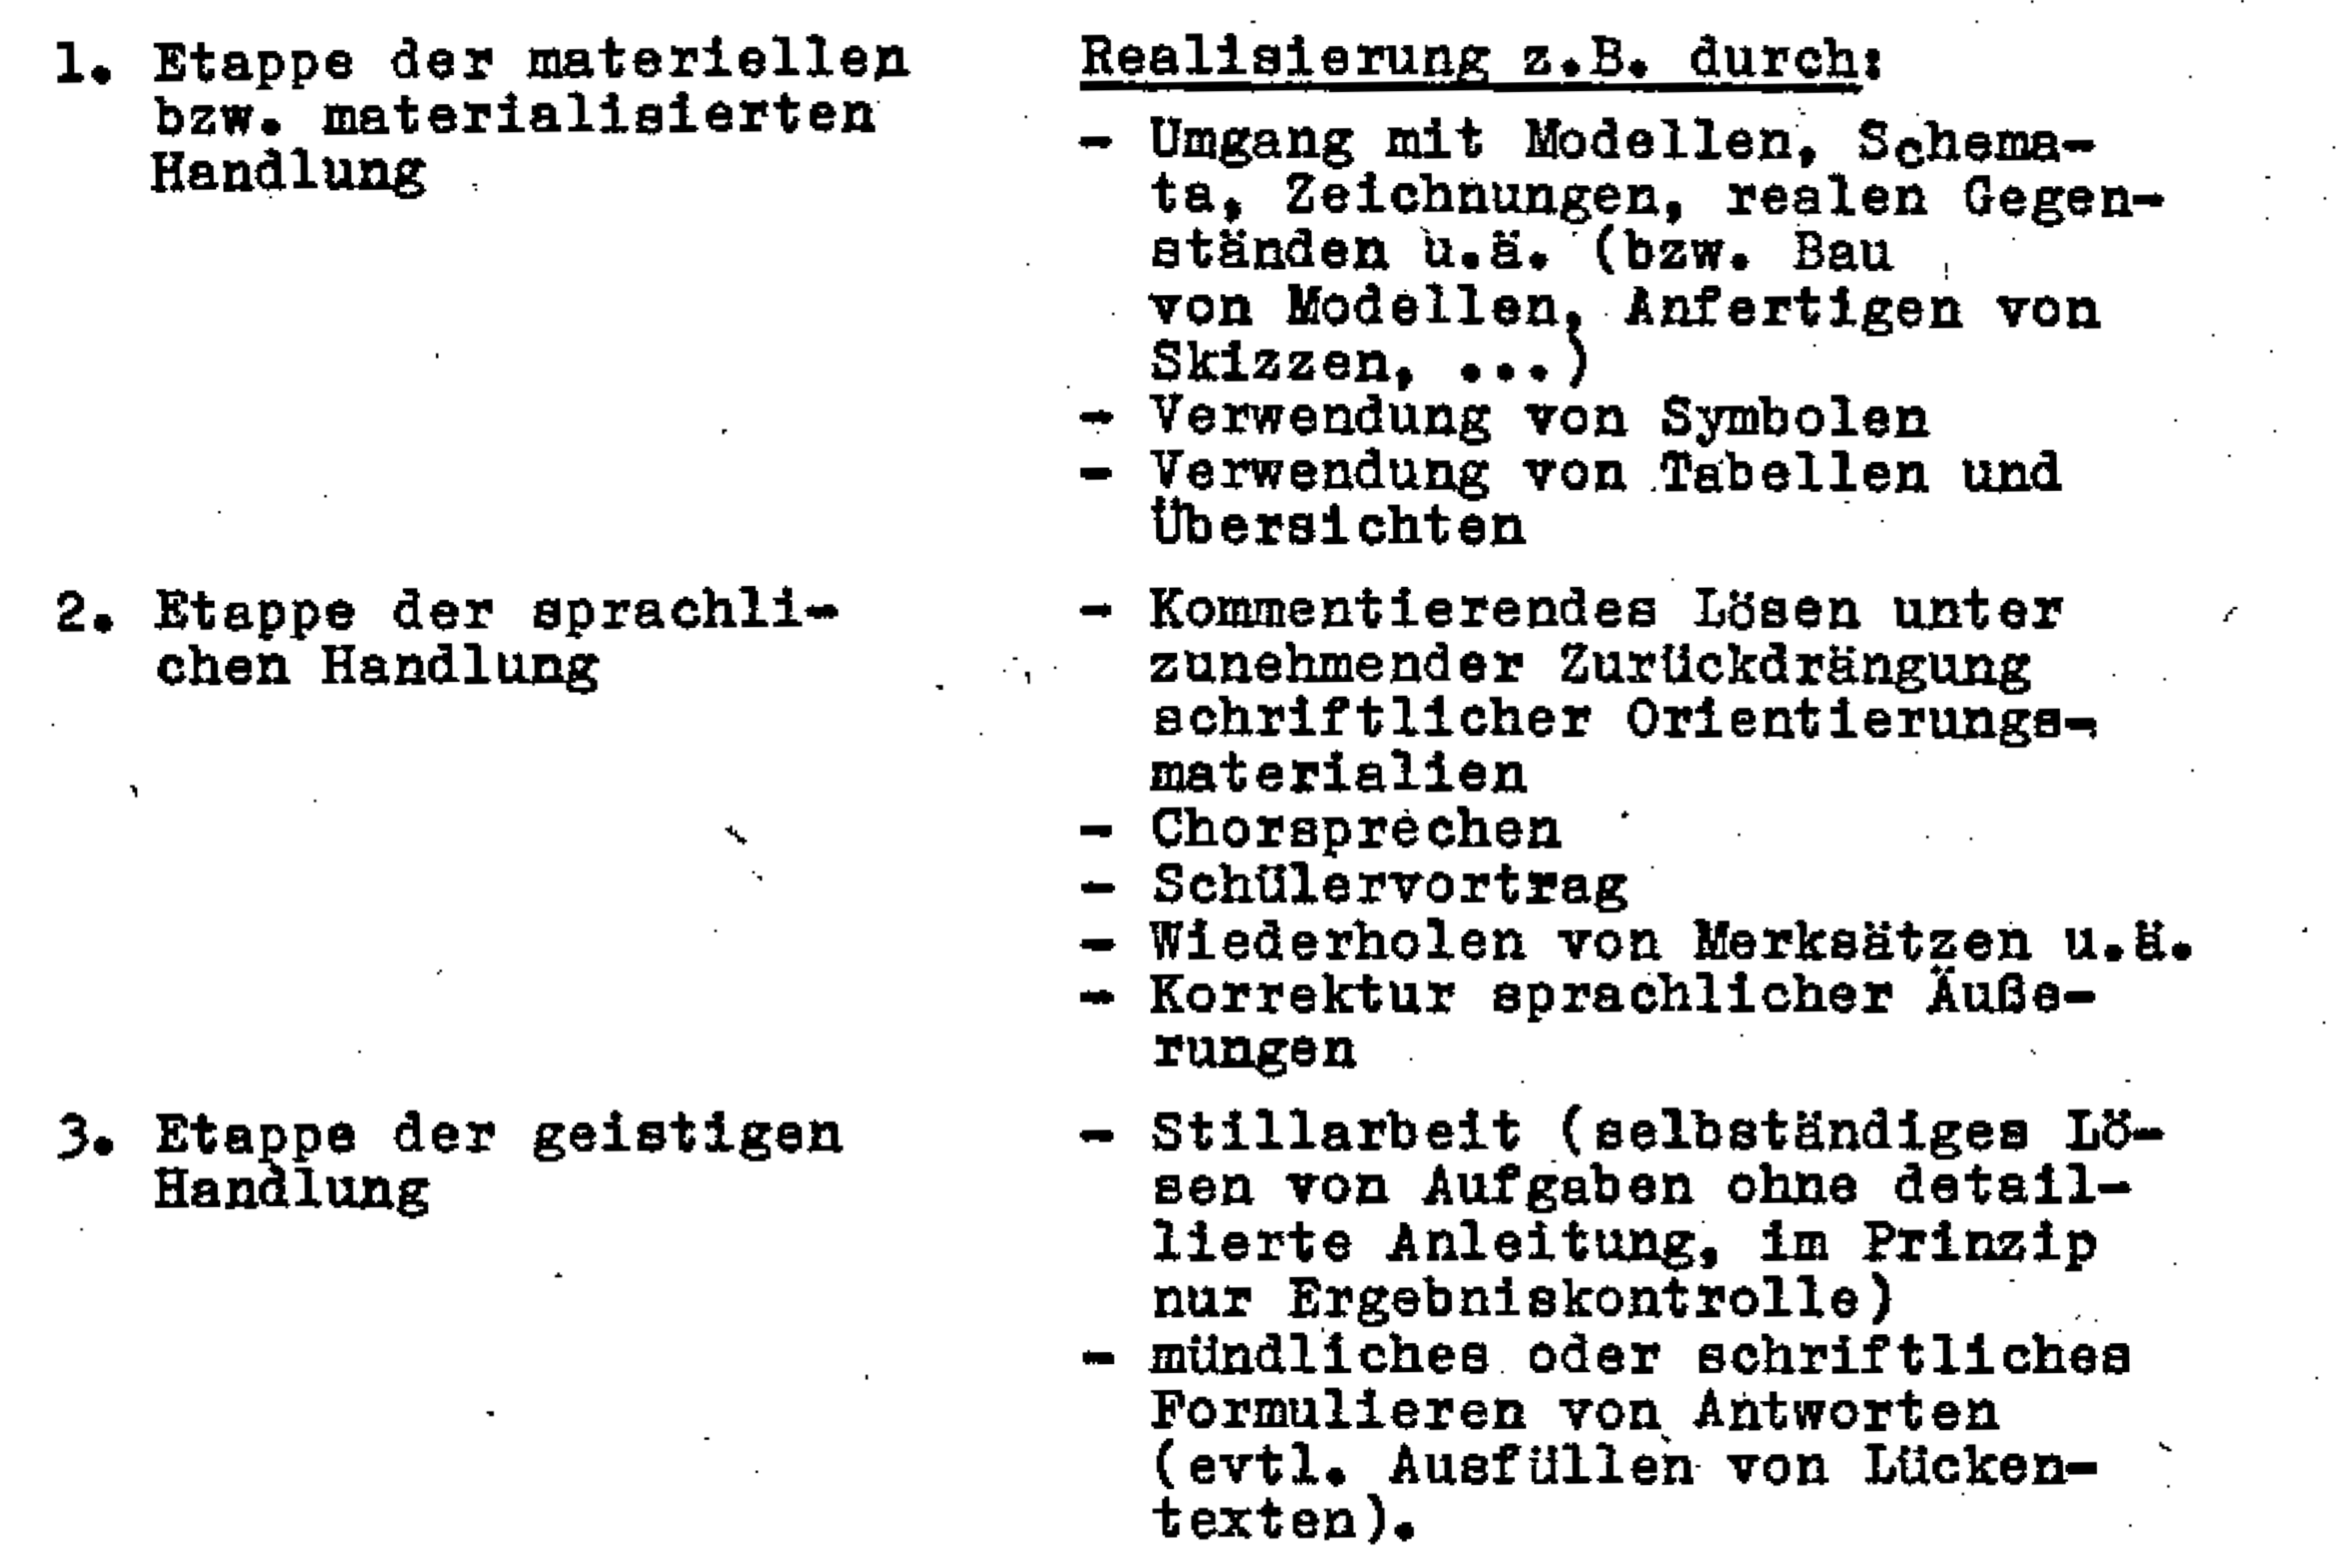
\includegraphics[width=0.9\linewidth]{pictures/6-Etappen} 

}

\caption{Beispiele zur etappenweisen Verinnerlichung von Handlungen im Mathematikunterricht nach Steinhöfel et al. (\citeproc{ref-Steinhofel1988}{1988, S. 19})}\label{fig:Etappen}
\end{figure}

Besonders bedeutsam sind derartige Verinnerlichungsprozesse für die \emph{elementaren Aneignunghandlungen} \textbf{Identifizieren und Realisieren} (vgl. Abschnitt ®ref(elementare-aneignungshandlungen). Derartige Handlungen sollten also direkter \textbf{Bestandteil der Stoffvermittlung} sein und nicht dem zufälligen Erwerb in anschließenden Übungsphasen überlassen werden.

\section{Festigung}\label{festigung}

Ist eine sogenannte \emph{Erstaneignung} eines Lerngegenstands erfolgt, kann dieser nun \textbf{gefestigt} werden. Hierzu sind sowohl automatisierende als auch produktive Übungen\footnote{Mehr dazu finden Sie z.~B. im \href{https://stoffdidaktik.heiko-etzold.de/2022/8-aufgabengestaltung.html\#produktives-üben}{Stoffdidaktik-Skript von 2022/23}.} notwendig. Steinhöfel et al. (\citeproc{ref-Steinhofel1988}{1988, S. 34}) schlagen hierfür verschiedene Maßnahmen zum Umgang mit dem Lerngegenstand vor:

\begin{itemize}
\tightlist
\item
  Verwendung von Spezial- und Extremfällen\\
\item
  Umformulieren, Bedingungen variieren, Umkehrungen bilden\\
\item
  Verwendung unterschiedlicher Bezeichnungen\\
\item
  Bekanntes Neuem gegenüberstellen und Zusammenhänge erkennen lassen
\end{itemize}

Im Sinne der Typisierung von Lernhandlungen (siehe Abschnitt \ref{typische-lernhandlungen}) bezieht sich dies v.~a. auf \emph{Grundhandlungen} und \emph{komplexe Handlungen}.

\section{Handlungskontrolle}\label{handlungskontrolle}

Die Handlungsausführung sollte stets von einer \textbf{Handlungskontrolle} begleitet werden. Das bedeutet, dass die Schülerinnen und Schüler eine bewusste Beziehung herstellen zwischen ihren (erreichten oder zu erreichenden) Handlungsergebnissen, den eingesetzten Lernmitteln sowie deren Bedingungen und der eigenen Handlungsausführung.
Die Handlungskontrolle ist dabei eine \emph{Selbstkontrolle} und muss dementsprechend auch erst einmal ausgebildet werden. Folgende methodischen Maßnahmen scheinen hierfür hilfreich zu sein:

\begin{itemize}
\item
  Ein Abgleich mit den zu erreichenden Handlungsergebnissen ist nur möglich, wenn im Vorfeld eine Zielklarheit besteht. Daher ist es so wichtig, die \textbf{Lernziele explizit zu formulieren und auch festzuhalten}.
\item
  Durch das \textbf{Anfertigen eines Lernprotokolls} (vgl. \citeproc{ref-Bruder2011}{Bruder, 2001}) erhalten die Schülerinnen und Schüler eine Möglichkeit, ihre eigenen Lernhandlungen und -ergebnisse zu dokumentieren und nachzuvollziehen. Insbesondere kann in diesem auch ohne jeglichen Bewertungsdruck dargestellt werden, wo man selbst als Schülerin oder Schüler noch Lücken sieht bzw. was man noch nicht verstanden hat.
\item
  Als weitere effektive Maßnahme in der Ausbildung der Handlungskontrolle hat sich die \textbf{gegenseitige Kontrolle der Schülerinnen und Schüler} als hilfreich herausgestellt. »Es läßt sich zunächst beim Partner leichter feststellen als bei sich selbst, inwieweit ein Handlungsergebnis bestimmten Zielkriterien entspricht, die Handlungsausführung anforderungs- und regelgerecht erfolgt, wo Abweichungen und Fehler liegen und worin die Ursachen dafür bestehen können« (\citeproc{ref-Lompscher1985a}{Lompscher, 1983, S. 72}). Durch Verinnerlichung dieses Vorgehens kann dann schrittweise auch eine Selbstkontrolle erfolgen.
\end{itemize}

Die Handlungskontrolle leistet damit einen Beitrag, die Schülerinnen und Schüler langfristig zu einer Feldorientierung über den Lerngegenstand zu befähigen.

\section{Bezüge zur Stoffdidaktik}\label{bezuege-zur-stoffdidaktik-lernhandlungen}

\begin{itemize}
\item
  Die \textbf{etappenweise Verinnerlichung von Handlungen} kann dabei unterstützen, \textcolor{semanticColor}{**Grundvorstellungen aufzubauen**}. Das in Abb. \ref{fig:GVverinnerlichen} dargestellte Phasenmodell von Wartha \& Schulz (\citeproc{ref-Wartha2011}{2011, S. 11}) erinnert stark an die etappenweise Verinnerlichung von Lernhandlungen nach Gal'perin. Dabei verwendete \textcolor{semanticColor}{**Arbeitsmittel**} und \textcolor{semanticColor}{**Repräsentationen**} können als \textbf{Orientierungshilfe} dienen und unterstützen die Aneignung.
\item
  In der \textbf{Handlungskontrolle} wird über den Abgleich zwischen Handlungszielen, -durchführung und -ergebnissen die \textcolor{concreteColor}{**Kernidee in der Rückschauperspektive**} aufgegriffen.
\end{itemize}

Insgesamt ergeben sich aus den Überlegungen \textbf{typische Unterrichtssituationen}. Abbildung \ref{fig:Unterrichtsphasen} zeigt diese in Anlehnung an Bruder (\citeproc{ref-Bruder1991}{1991}) mit ihrem Zusammenhang zu den stoffdidaktichen Theoriebestandteilen.



\begin{figure}

{\centering 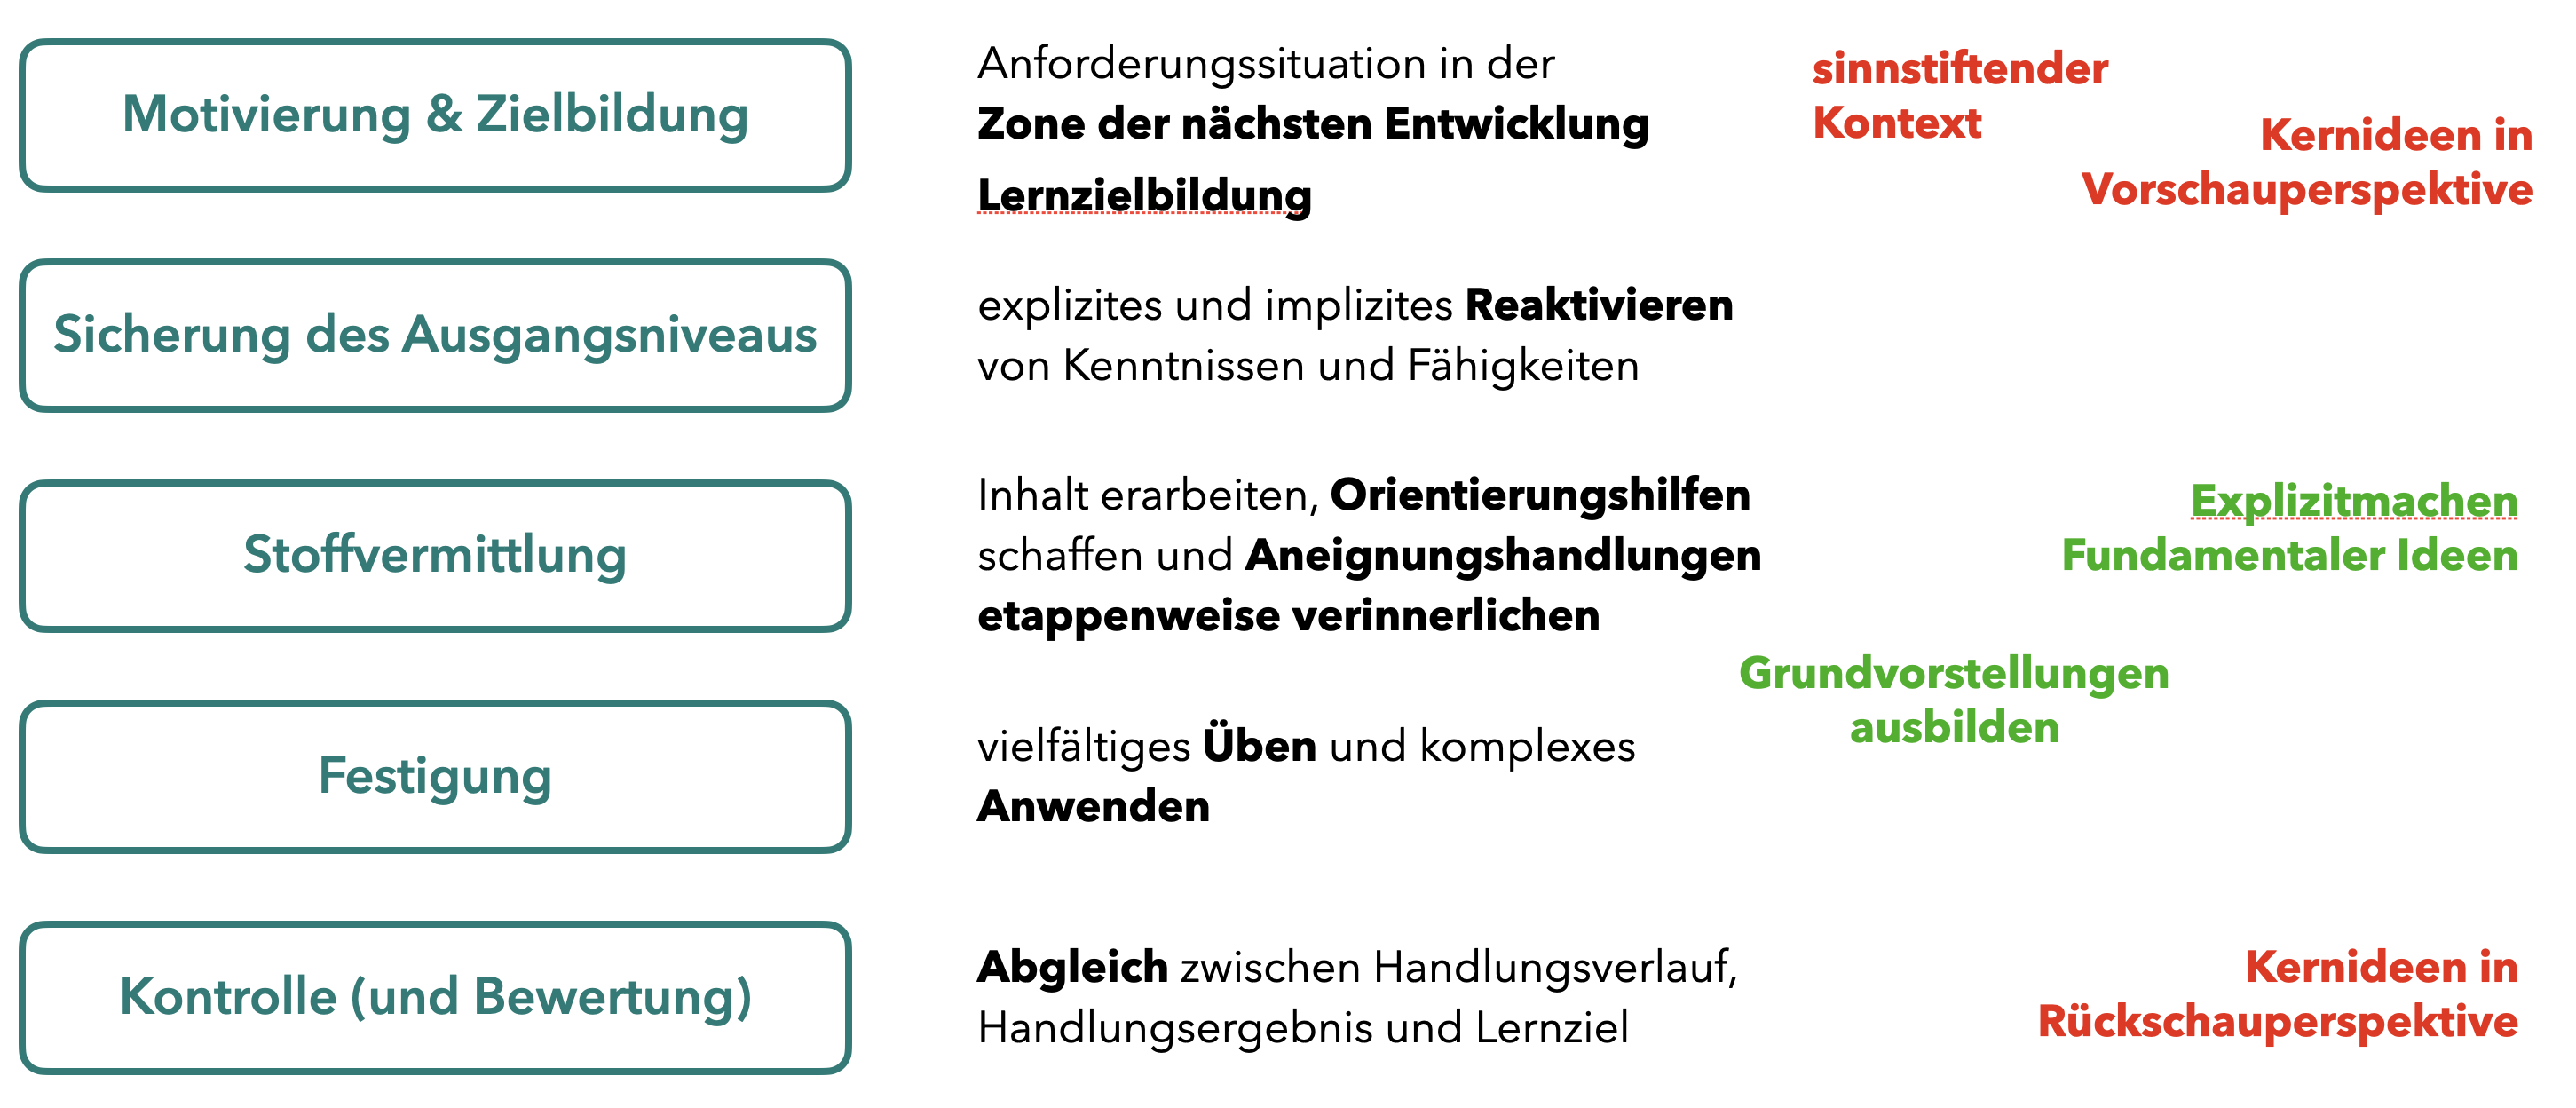
\includegraphics[width=0.95\linewidth]{pictures/6-Unterrichtssituationen} 

}

\caption{Typische Unterrichtssituationen nach Bruder (\citeproc{ref-Bruder1991}{1991})}\label{fig:Unterrichtsphasen}
\end{figure}

Im nächsten Kapitel wird -- aufgeschlüsselt nach Begriffen, Zusammenhängen und Verfahren -- insbesondere dargestellt, wie Stoffvermittlung und Festigung allgemein gestaltet werden können.
All diese Überlegungen sind jedoch nicht als starres Unterrichtsvorgehen aufzufassen, sondern sollen vielmehr Ihnen als Lehrkraft wiederum eine \emph{Orientierung} bieten, Ihren Unterricht zu strukturieren und entsprechende Lernumgebungen zu gestalten.

\chapter{Begriffe, Zusammenhänge, Verfahren}\label{begriffe-zusammenhuxe4nge-verfahren}

\begin{quote}
\textbf{Ziele}

\begin{itemize}
\tightlist
\item
  Sie kennen prinzipielle Möglichkeiten, Begriffe, Zusammenhänge und Verfahren einzuführen, Aneignungsprozesse mithilfe von Orientierungshilfen zu gestalten und die Inhalte zu festigen.\\
\item
  Sie erkennen Gemeinsamkeiten und Unterschiede in den typischen Vorgehensweisen für Begriffe, Zusammenhänge und Verfahren.\\
\item
  Sie können die Prozesse tätigkeitstheoretisch einordnen.
\end{itemize}

\textbf{Material}

\begin{itemize}
\tightlist
\item
  Folien zum Kapitel 7 (\href{files/Stoffdidaktik2024-07-BegriffeZusammenhaengeVerfahren.pdf}{pdf}, \href{files/Stoffdidaktik2024-07-BegriffeZusammenhaengeVerfahren.key}{Keynote})
\end{itemize}
\end{quote}

Aufbauend auf den tätigkeitstheoretischen Grundlagen der letzten beiden Kapitel soll in diesem Kapitel dargestellt werden, wie damit das Unterrichten von Begriffen, Zusammenhängen und Verfahren gestaltet werden kann. Dabei wird immer von drei Schritten ausgegangen:

\begin{enumerate}
\def\labelenumi{\arabic{enumi}.}
\tightlist
\item
  Begriff/Zusammenhang/Verfahren \textbf{erarbeiten}\\
\item
  Begriff/Zusammenhang/Verfahren \textbf{aneignen} über die Nutzung geeigneter Orientierungshilfen sowie der etappenweisen Ausbildung geistiger Handlungen\\
\item
  Begriff/Zusammenhang/Verfahren \textbf{festigen}
\end{enumerate}

Perspektivisch sollten Sie in der Lage sein, die hier beschriebenen Prozesse auf konkrete Lerngegenstände anzuwenden. Dabei ist jedoch zu beachten, dass es sich \emph{nicht} um eine \emph{feste Vorgehensweise} handelt, sondern vielmehr \emph{prinzipielle Gestaltungsmöglichkeiten} für die Stofferarbeitung und Festigung beschrieben werden.

\section{Begriffe}\label{begriffe}

»Man spricht allgemein von einem ›Begriff‹, wenn eine Anzahl von Objekten oder Ereignissen aufgrund gewisser übereinstimmender Merkmale mit einem gemeinsamen Namen belegt wird« (Weinert, 1974, S.~664, zitiert nach \citeproc{ref-Zech1998}{Zech, 1998, S. 165}).

Damit werden zwei Dimensionen von Begriffen sichtbar, nämlich der \textbf{Bezeichner} und das \textbf{Bezeichnete}. Während der Bezeichner das \emph{Wort} bzw. der \emph{Name} ist, mit dem das zu betrachtende Objekt oder Ereignis belegt wird, ist das Bezeichnete die \emph{Idee} hinter dem Objekt, also das Gefüge an \emph{übereinstimmenden Merkmalen}. Weder \emph{Bezeichner} noch \emph{Bezeichnetes} sind jedoch das Objekt oder Ereignis selbst.
Äquivalente, und auch in den Sprachwissenschaften bedeutsame Bezeichnungen sind \textbf{Signifikant} für den Bezeichner und \textbf{Signifikat} für das Bezeichnete (vgl. auch \citeproc{ref-Rembowski2015}{Rembowski, 2015, 13~ff.}; \citeproc{ref-dewiki:214582005}{Wikipedia, 2021c}, \citeproc{ref-dewiki:212433603}{2021b}).

Wenn etwa ein Kind den Bezeichner \emph{Quader} verwendet, um ein Viereck mit vier gleich langen Seiten und vier rechten Winkeln zu beschreiben (also eigentlich das Bezeichnete eines \emph{Quadrates} meint), kann es sich hier durchaus um eine Wortverwechslung handeln, die nicht zwingend mit einem inhaltlichen Fehlverständnis einhergehen muss.

\subsection{Begriffe bilden}\label{begriffe-bilden}

Die Einführung von Begriffen kann stets als Wechselspiel zwischen \textbf{Beispielen/Gegenbeispielen} und der \textbf{Begriffsfestlegung} aufgefasst werden. Die Richtung und Qualität dieses Zusammenhangs ermöglicht verschiedene Wege zum Begriff (siehe Abbildung \ref{fig:Begriffseinfuehrung}).

\begin{figure}

{\centering 
\includegraphics[width=0.75\linewidth]{pictures/7-Begriffe} 

}

\caption{Möglichkeiten der Begriffseinführung}\label{fig:Begriffseinfuehrung}
\end{figure}

\subsubsection{Ostensive Begriffseinführung}\label{ostensive-begriffseinfuxfchrung}

Bei der ostensiven Begriffseinführung wird das Lernen eines Begriffs als \textbf{Erfassen der Gestalt} als einprägsames Ganzes angenommen. Das heißt, der Begriff wird gar nicht formal definiert, sondern nur über Beispiele dargestellt. Dies wird insbesondere bei Arbeitsbegriffen so gehandhabt (z.~B. \emph{Bruchstrich}) oder bei der Begriffseinführung in der Grundschule, wenn deren Gestalt leicht eingänglich ist (z.~B. \emph{Kreis}).

Dabei muss jedoch die \textbf{wahrgenommene Gestalt dem Wesentlichen} des Begriffs entsprechen und der \textbf{Gestalteindruck ist häufig abhängig von der Lage}. Es ist also darauf zu achten, nicht ausschließlich Spezialfälle zu präsentieren, die dann zu einer Untergeneralisierung des Begriffs führen. Werden z.~B. zwei \emph{zueinenander senkrechte} Strecken präsentiert, sollten diese also nicht gleich lang sein, sich nicht in der Mitte schneiden und auch nicht parallel zu den Tafel-/Blatt-/Bildschirmrändern ausgerichtet sein (siehe Abbildung \ref{fig:SenkrechtOstensiv}).



\begin{figure}

{\centering 
\includegraphics[width=0.5\linewidth]{pictures/7-senkrecht} 

}

\caption{Ungeeignete und geeignete ostensive Darstellung des Begriffs \emph{senkrecht zueinander}}\label{fig:SenkrechtOstensiv}
\end{figure}

\subsubsection{Induktive Begriffseinführung}\label{induktive-begriffseinfuxfchrung}

Bei der induktiven Begriffseinführung wird zunächst eine \textbf{Vielzahl an Beispielen} präsentiert. Aus diesen heraus wird dann das \textbf{Wesentliche des Begriffs extrahiert}. Dafür werden die Objekte zunächst beschrieben und anschließend gemeinsame Eigenschaften entdeckt. Dies kann passieren, indem die ungeordneten Beispiele nach Merkmalen sortieren werden oder bereits in Teilmengen aufgeteilt präsentiert werden. Daran wird nun der Begriffsinhalt herausgearbeitet.

Dieses Vorgehen ist relativ natürlich, da es auch der Begriffsbildung im Vorschulalter bzw. im Alltag entspricht. Allerdings benötigt es sehr viel Zeit. Hinzu kommt, dass das Erkennen der gemeinsamen Merkmale in der Unterrichtssituation nicht selten zu einem \emph{Ostereiersuchen} verfällt, indem die Lehrkraft so lange nachfragt, bis die gewünschte Eigenschaft gefunden wird. Oder noch kritischer formuliert: »Die Lernenden jedoch haben noch keine Ahnung von diesem Wesen und können sie auch nicht gewinnen, da sie keinerlei Mittel dafür besitzen« (\citeproc{ref-Giest2004a}{Giest \& Lompscher, 2004}).

Beim Einsatz der induktiven Begriffseinführung müssen also insbesondere geeignete Impulsfragen im Vorhinein bedacht werden, um die Schülerinnen und Schüler durch gezielte Fragestellungen das Wesentliche des Begriffs entdecken lassen zu können.

\subsubsection{Deduktive Begriffseinführung}\label{deduktive-begriffseinfuxfchrung}

Die deduktive Begriffseinführung geht den Weg \textbf{von der Definition zu den Beispielen}. Dieses Vorgehen ist das übliche in der Hochschulmathematik und sollte -- um zum Beispiel wissenschaftspropädeutisch tätig zu sein -- auch im Schulunterricht schon vermittelt werden.

Typische Impulsfragen für das anschließende Identifizieren udn Realisieren von Repräsentanten\footnote{Diese \emph{Repräsentanten} eines Begriffs sind nicht mit dessen \emph{Repräsentationen} im Sinne der Grundvorstellungsidee zu verwechseln! Die Repräsentanten sind konkrete (reale oder ideelle) Objekte, Repräsentationen dagegen Darstellungen, die ein operatives Arbeiten ermöglichen. Beides kann aber natürlich sehr ähnlich aussehen oder sogar zusammenfallen.} bei der deduktiven Begriffseinführung nach Gabe der Definition zu unterstützen, können sein:

\begin{itemize}
\tightlist
\item
  Ist das ein \ldots?
\item
  Stelle ein \ldots{} her.
\item
  Welche Teile der Definition sind nicht erfüllt?
\item
  Was muss an dem \ldots{} verändert werden, damit es ein \ldots{} ist?
\item
  Wie prüft man, ob das ein \ldots{} ist?
\item
  Warum entsteht ein \ldots, wenn man das so und so herstellt?
\end{itemize}

\subsubsection{Aufsteigen vom Abstrakten zum Konkreten}\label{aufsteigen-vom-abstrakten-zum-konkreten}

Das Aufsteigen vom Abstakten zum Konkreten ist durch ein spezifisches \textbf{Wechselspiel von einem Beispiel, der Definition und weiterer Beispiele} geprägt. Nach Lompscher (\citeproc{ref-Lompscher1996}{1996}) sind drei Schritte relevant.

\begin{figure}

{\centering 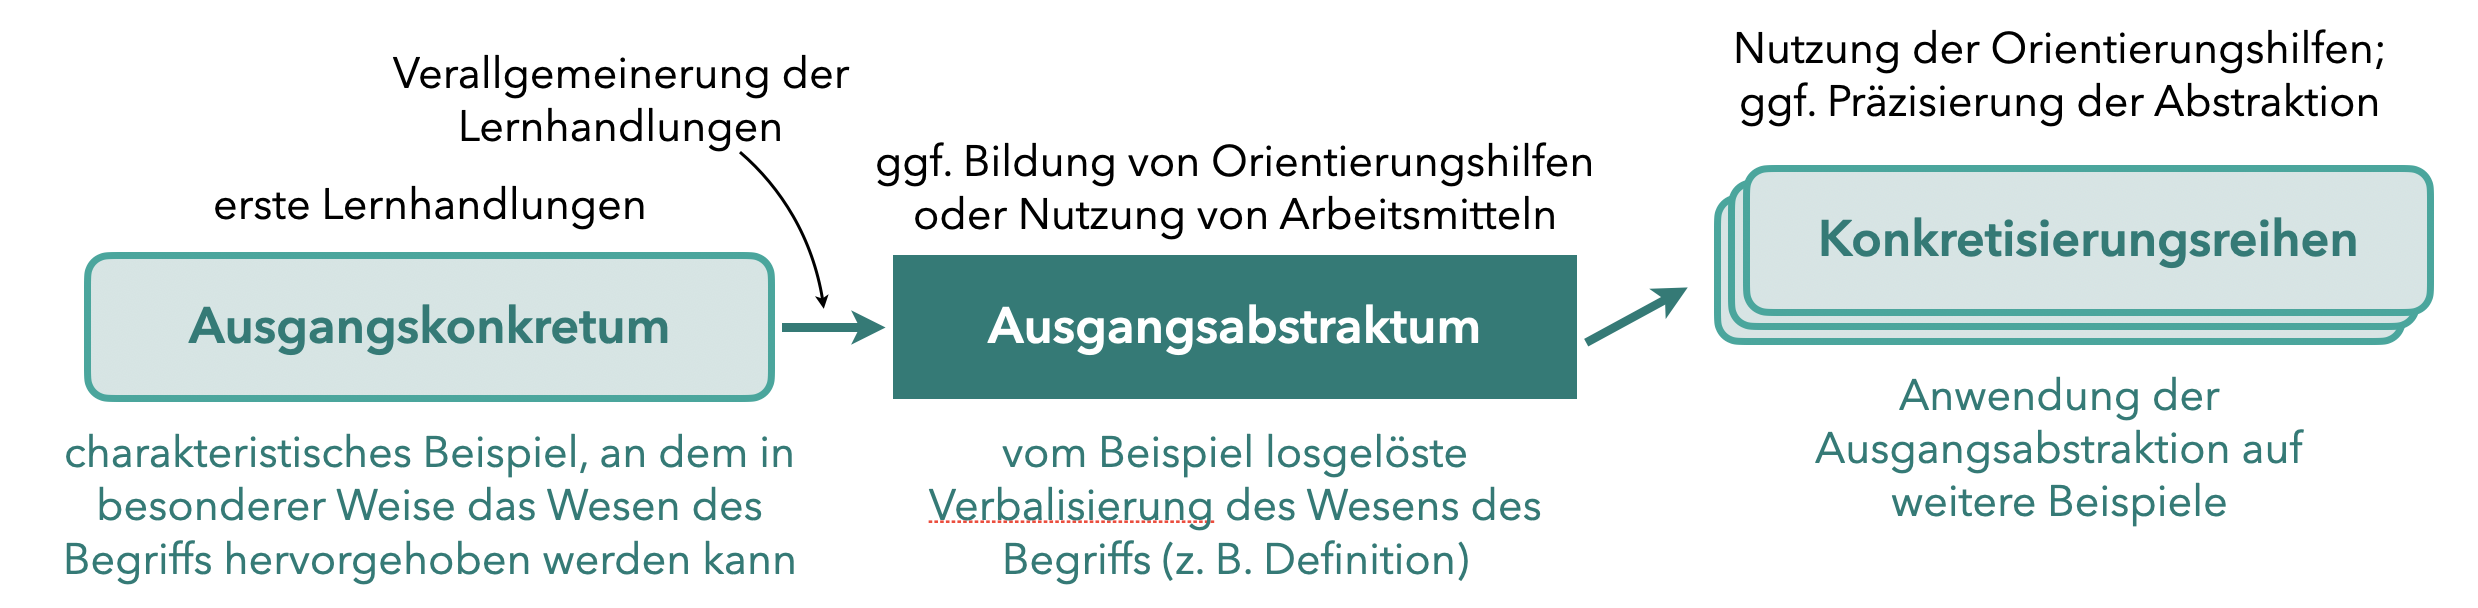
\includegraphics[width=0.9\linewidth]{pictures/7-AK} 

}

\caption{Aufsteigen vom Abstrakten zum Konkreten}\label{fig:AK}
\end{figure}

\begin{enumerate}
\def\labelenumi{\arabic{enumi}.}
\item
  Für die Einführung des Begriffs wird ein konkretes Ausgangsbeispiel gewählt, an dem das Wesen des Begriffs besonders gut deutlich wird. An diesem \textbf{Ausgangskonkretum} werden Lernhandlungen erarbeitet, die sich zwar am Beispiel orientieren, aber verallgemeinern lassen, sodass sie dem Begriffsaufbau dienlich sind.
\item
  Im Anschluss wird, mit Unterstützung der Lehrkraft, das Wesen des Begriffs herausgearbeitet und in Form einer \textbf{Ausgangsabstraktion} formuliert. Dieses Vorgehen ist vergleichbar mit dem induktiven Begriffserwerb, allerdings wird nicht aus einer Vielzahl von Beispielen eine gemeinsame Eigenschaft eliminiert, sondern am charakteristischen Beispiel wird die Eigenschaft durch eine wissende Person (Lehrkraft) in Bezug auf die Handlungserfahrungen der Schülerinnen und Schüler dargestellt. Dieser Prozess kann durch Orientierungshilfen oder Arbeitsmittel (siehe nächstes Kapitel) unterstützt werden.
\item
  Der dritte Schritt, das eigentliche Aufsteigen vom Abstrakten zum Konkreten, ist nun das Abarbeiten von \textbf{Konkretisierungsreihen}. Hierzu werden weitere Beispiele für den Begriff betrachtet, auf die das Ausgangsabstraktum angewandt wird. Orientierungshilfen/Arbeitsmittel dienen dabei als Mittler und die Lernhandlungen werden in verallgemeinerter und ggf. auch modifizierter Form angewandt. Erst auf diese Weise ist ein echtes Durchdringen des Begriffs möglich. Dieses Vorgehen ist mit dem deduktiven Vorgehen vergleichbar, allerdings nicht im dem Sinne, dass aus einer Definition heraus die Beispiele generiert werden. Vielmehr wird auf gegebene Beispiele die Definition angewandt, ausgeschärft und damit der Begriff immer besser verstanden.
\end{enumerate}

Diese Vorgehensweise hat den Vorteil, \textbf{relativ effektiv} zu sein und trotz des Verzichts auf ein deduktives Vorgehen recht schnell zu einer (ersten) Definition des Begriff zu kommen. Außerdem ist sie \textbf{ehrlich gegenüber den noch nicht vorhandenen Kenntnissen der Schülerinnen und Schüler}, da diese bei einem induktiven Vorgehen i.~d.~R. noch nicht wissen, nach welchem gemeinsamen Merkmal die Beispiele nun analysiert werden sollen, so dass es oft mit einem Raten (oder letztlich doch einer Vorgabe durch die Lehrkraft) verbunden ist, auf das zu interessierende Merkmal zu stoßen.

\subsubsection{Beispiele und Gegenbeispiele}\label{beispiele-und-gegenbeispiele}

Unabhängig davon, auf welche Art und Weise man Begriffe einführt, ist stets ein Zusammenspiel aus Beispielen, Gegenbeispielen und verbalen Erläuterungen notwendig -- und das in allen Altersklassen! Bei entsprechenden Verbalisierungen sind ggf. weniger Beispiele/Gegenbeispiele nötig, da damit das Wesen des Begriffs besser herausgearbeitet werden kann (\citeproc{ref-Zech1998}{Zech, 1998, S. 260}).

Bei der Auswahl von Beispielen und Gegenbeispielen bieten sich das \textbf{Variationsprinzip} und das \textbf{Kontrastprinzip} an. Die folgenden Überlegungen stammen hauptsächlich von Zech (\citeproc{ref-Zech1998}{1998, 260~ff.}).

\paragraph{Variationsprinzip}\label{variationsprinzip}

Beispiele sollten breit variiert werden, es darf nicht zu einer Untergeneralisierung kommen. Im Alltag als Gegenbeispiele empfundene Beispiele müssen mit angebracht werden. Wichtig erscheinende \textbf{irrelevante Merkmale} sollten mindestens einmal \textbf{variiert} werden.

Für den Rechtecktbegriff kann dies eine Variation in Größe, Seitenverhältnis, Ausrichtung und Farbe, aber auch die Präsentation von Spezialfällen (z.~B. eines Quadrates) bedeuten (siehe Abbildung \ref{fig:VariationRechteck}).



\begin{figure}

{\centering 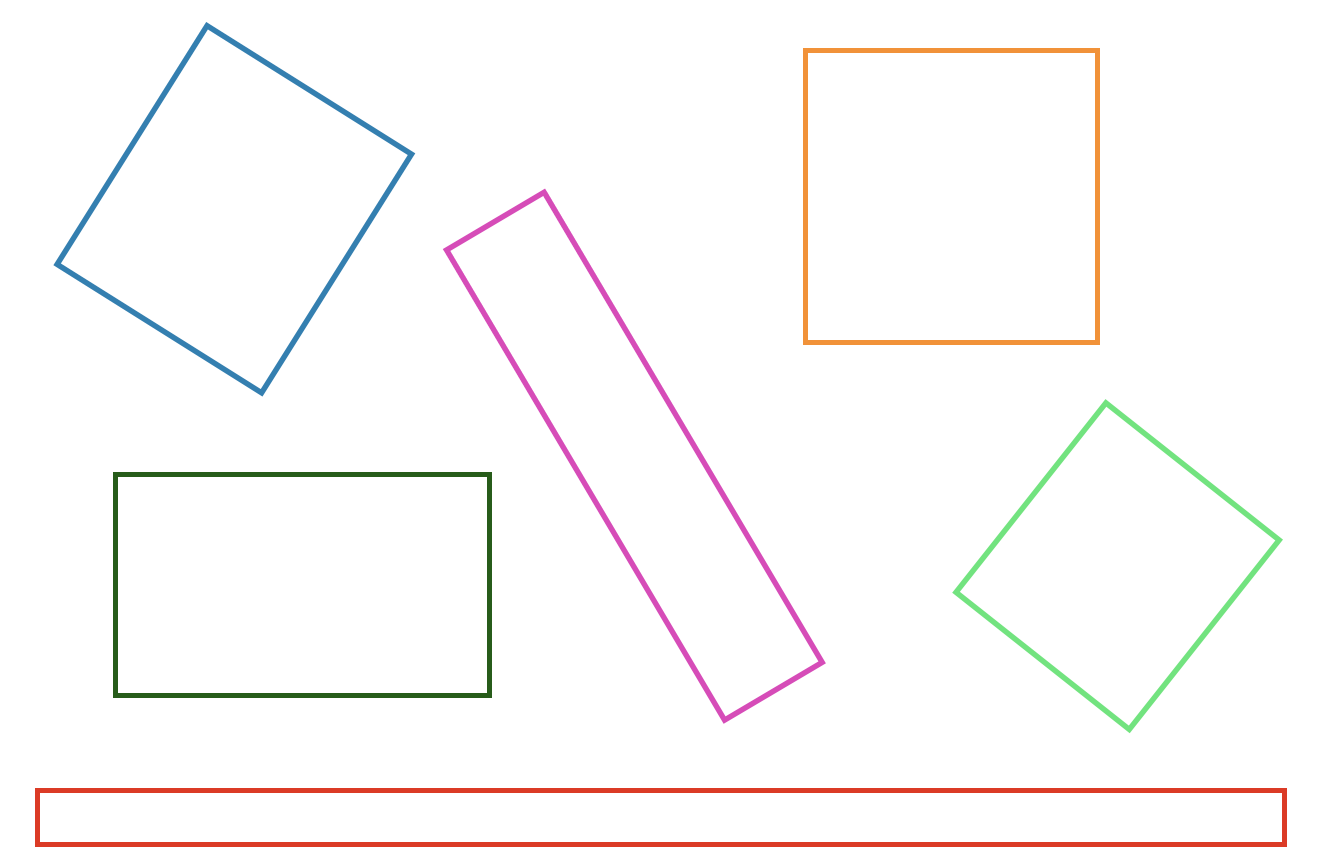
\includegraphics[width=0.75\linewidth]{pictures/7-Variation} 

}

\caption{Variationsprinzip beim Begriff \emph{Rechteck}}\label{fig:VariationRechteck}
\end{figure}

Um dieses Prinzip für einen Begriff zu realisieren, muss man sich als Lehrkraft also Gedanken über die mathematisch relevanten und irrelevanten Eigenschaften machen. Auch eine explizite Diskussion mit den Schülerinnen und Schülern, warum diese Eigenschaften variiert werden durften (und andere nicht), kann hilfreich für das Begriffsverständnis sein.

\paragraph{Kontrastprinzip}\label{kontrastprinzip}

Gegenbeispiele dürfen nicht für Beispiele gehalten werden, es darf nicht zu einer Übergeneralisierung kommen. Im Alltag als Beispiele empfundene Gegenbeispiele (sogenannte \emph{Fastbeispiele}) müssen diskutiert werden. \textbf{Relevante Merkmale} müssen mindestens einmal \textbf{fehlen}.

Für den Rechteckbegriff relevant sind etwa die rechten Winkel (was bei Beibehaltung der gleich langen, parallelen Seiten zu einem Parallelogramm führt). Auch die \emph{Ecken}-Eigenschaften und die Tatsache, dass es sich um eine Figur (und nicht um einen Körper) handelt, sind relevant (siehe Abbildung \ref{fig:KontrasRechteck}).



\begin{figure}

{\centering 
\includegraphics[width=0.5\linewidth]{pictures/7-Kontrast} 

}

\caption{Kontrastprinzip beim Begriff \emph{Rechteck}}\label{fig:KontrasRechteck}
\end{figure}

\paragraph{Darbietung von Beispielen und Gegenbeispielen}\label{darbietung-von-beispielen-und-gegenbeispielen}

Zech (\citeproc{ref-Zech1998}{1998, S. 261}) fasst zusammen: \textbf{»Beispiele und Gegenbeispiele sind dann am effektivsten, wenn sich die Beispiele möglichst stark in den irrelevanten Merkmalen unterscheiden und die Gegenbeispiele in möglichst wenigen relevanten Merkmalen unterscheiden.«}

Eine simultane Darbietung zweier stark kontrastierender Beispiele (Abbildung \ref{fig:SimultanBeispiel}) oder eines Beispiels mit einem sehr ähnlichen Gegenbeispiel (Abbildung \ref{fig:SimultanGegenbeispiel}) kann weiterhin den Fokus auf die relevanten Merkmale des Begriffs lenken.



\begin{figure}

{\centering 
\includegraphics[width=0.5\linewidth]{pictures/7-Quadrat} 

}

\caption{Simultane Darbietung zweier Beispiele zum Begriff \emph{Quadrat}}\label{fig:SimultanBeispiel}
\end{figure}



\begin{figure}

{\centering 
\includegraphics[width=0.4\linewidth]{pictures/7-Achsensymmetrie} 

}

\caption{Simultane Darbietung von Beispiel und Gegenbeispiel zum Begriff \emph{Achsensymmetrie}}\label{fig:SimultanGegenbeispiel}
\end{figure}

\subsection{Begriffe aneignen}\label{begriffe-aneignen}

Die relevanten Aneignungshandlungen beim Begriffserwerb sind das \textbf{Identifizieren} und \textbf{Realisieren}. Die Tabelle konkretisiert die Möglichkeit der Gestaltung von Orientierungshilfen und das etappenweise Ausbilden geistiger Handlungen an diesen beiden Aneignungshandlungen.

\begin{longtable}[]{@{}
  >{\raggedright\arraybackslash}p{(\columnwidth - 4\tabcolsep) * \real{0.2000}}
  >{\raggedright\arraybackslash}p{(\columnwidth - 4\tabcolsep) * \real{0.4000}}
  >{\raggedright\arraybackslash}p{(\columnwidth - 4\tabcolsep) * \real{0.4000}}@{}}
\caption{\label{tab:begriffsschritte} Teilprozesse zur Begriffsbildung und -aneignung, nach Steinhöfel et al. (\citeproc{ref-Steinhofel1988}{1988, S. 46})}\tabularnewline
\toprule\noalign{}
\begin{minipage}[b]{\linewidth}\raggedright
\end{minipage} & \begin{minipage}[b]{\linewidth}\raggedright
Identifizieren
\end{minipage} & \begin{minipage}[b]{\linewidth}\raggedright
Realisieren
\end{minipage} \\
\midrule\noalign{}
\endfirsthead
\toprule\noalign{}
\begin{minipage}[b]{\linewidth}\raggedright
\end{minipage} & \begin{minipage}[b]{\linewidth}\raggedright
Identifizieren
\end{minipage} & \begin{minipage}[b]{\linewidth}\raggedright
Realisieren
\end{minipage} \\
\midrule\noalign{}
\endhead
\bottomrule\noalign{}
\endlastfoot
\textbf{Orientierungshilfen} & System der Merkmale des Begriffs; Schrittfolge zum Prüfen der Merkmale & Handlungsvorschrift zum Herstellen oder Vervollständigen des Objekts \\
\textbf{Etappe der materiellen/materialisierten Handlung} & Überprüfung der Merkmale an gegebenen Objekten oder an Modellen (Zeichnungen, Diagramme); Orientierungshilfe liegt schriftlich vor & Beim Lösen entsprechender Aufgaben orientieren sich Schülerinnen und Schüler am Text der Handlungsvorschrift, die schriftlich vorliegt. \\
\textbf{Etappe der sprachlichen Handlung} & sprachliches Begründen des Zutreffens oder Nichtzutreffens der einzelnen Merkmale (unter zunehmender Zurückdrängung der Orientierungshilfe) & Kommentieren des Lösungsweges beim Ausführen der Handlungsschritte (Handlungsvorschrift liegt nicht mehr vor) \\
\textbf{Etappe der geistigen Handlung} & sofortiges Entscheiden, ob der Begriff zutrifft oder nicht (ohne Benutzung der Orientierungshilfe) & selbstständiges Lösen entsprechender Aufgaben (ohne Verwendung der Handlungsvorschrift) \\
\end{longtable}

\subsection{Begriffe festigen}\label{begriffe-festigen}

Vertiefende Übungen ergeben sich v.~a. durch die Einordnung des neu erlernten Begriffs in ein \textbf{Begriffssystem}. Hinzu kommt die Verwendung \textbf{alternativer Definitionen} sowie die \textbf{Variablität in der Verwendung von Bezeichnungen} (z.~B. Variablen). Auch können \textbf{Grenz- und Sonderfälle} des Begriffs diskutiert werden, um ein vertieftes Verständnis zu gewinnen (vgl. \citeproc{ref-Steinhofel1988}{Steinhöfel et al., 1988, S. 34}). Eine systematische Übersicht, auch für ein ähnliches Vorgehen bei Sachverhalten und Verfahren, bietet Tabelle \ref{tab:festigen}.

Nach Vollrath \& Roth (\citeproc{ref-Vollrath2012}{2012, S. 48}) ist ein Begriff verstanden, wenn Schülerinnen und Schüler

\begin{itemize}
\tightlist
\item
  die Bezeichnung des Begriffs kennen,
\item
  Beispiele angeben und jeweils begründen können, weshalb es sich um ein Beispiel handelt,
\item
  begründen können, weshalb etwas nicht unter den Begriff fällt,
\item
  charakteristische Eigenschaften des Begriffs kennen,
\item
  Oberbegriffe, Unterbegriffe und Nachbarbegriffe kennen,
\item
  mit dem Begriff beim Argumentieren und Problemlösen arbeiten können.
\end{itemize}

\section{Zusammenhänge}\label{zusammenhuxe4nge}

Bei Zusammenhängen (also Regeln, Gesetzen und Sätzen) bietet es sich an, in der Erarbeitung zwischen dem \textbf{Finden des Zusammenhangs}, dem \textbf{Finden einer Begründung} und der \textbf{Darstellung der Begründung} zu unterscheiden.\footnote{Spezifischer sprechen einige Quellen auch von der \emph{Satzfindung}, \emph{Beweisfindung} und \emph{Beweisdarstellung}, z.~B. Steinhöfel et al. (\citeproc{ref-Steinhofel1988}{1988, S. 59})}
Im schulischen Kontext erfüllt eine Begründung i.~d.~R. nicht nur die Funktion, den Wahrheitsgehalt des Sachverhaltes zu sichern (diese Funktion hat ein Beweis v.~a. in der Fachmathematik), sondern über die Begründung den Sachverhalt besser zu verstehen, dessen innere Struktur nachzuvollziehen und mithilfe der Begründung über den Sachverhalt zu kommunizieren.
Während die ersten beiden Teilprozesse v.~a. der \emph{Erarbeitung} des Sachverhalts dienen, sind alle drei Teilprozesse notwendige Bestandteile für die \emph{Aneignung} des Sachverhalts.

\subsection{Zusammenhänge erarbeiten}\label{zusammenhuxe4nge-erarbeiten}

\subsubsection{Zusammenhänge finden}\label{zusammenhuxe4nge-finden}

Für das Finden neuer Zusammenhänge bestehen folgende Möglichkeiten (vgl. \citeproc{ref-Vollrath2012}{Vollrath \& Roth, 2012, 247~f.}):

\begin{itemize}
\item
  Der neue Zusammenhang wird \textbf{induktiv} über das Entdecken von Merkmalen in gegebenen Situationen erarbeitet.

  \begin{quote}
  Werden bspw. Rechtecke und ihre Diagonalen gezeichnet, kann daraus entdeckt werden, dass sich die Diagonalen stets halbieren, dies also ein gültiger Zusammenhang zu sein scheint.
  \end{quote}
\item
  Der neue Zusammenhang entsteht aus dem \textbf{Widerspruch zu einer angenommenen Hypothese}.

  \begin{quote}
  Aus dem Recheckbeispiel könnte angenommen werden, dass Vierecke mit sich halbierenden Diagonalen \emph{immer} Rechtecke sind. Über ein Gegenbeispiel kann aber gezeigt werden, dass dies auch bei Parallelogrammen der Fall ist. So wurde ein neuer Zusammenhang entdeckt.
  \end{quote}
\item
  Der neue Zusammenhang wird \textbf{deduktiv} aus bisherigen Zusammenhängen gefolgert.

  \begin{quote}
  Der Kosinussatz kann über die Zerteilung eines allgemeinen Dreiecks in rechtwinklige Dreiecke und die mehrfache Anwendung des Satzes des Pythagoras gefolgert werden.
  \end{quote}
\end{itemize}

Nicht immer ist es sinnvoll, einen Zusammenhang zu \emph{finden}. So kann etwa die Lösungsformel \(x_{1,2} = -\frac{p}{2}\pm \sqrt{\left(\frac{p}{2}\right)^2-q}\) schlecht \emph{vermutet} werden, um damit die Gleichung \(0 = x^2+px+q\) zu lösen. In dem Fall wird üblicherweise mithilfe einer \textbf{Herleitung} direkt zur Begründung des Zusammenhangs übergegangen. Ein solches Vorgehen ist i.~d.~R. deduktiv.

\subsubsection{Begründungen finden}\label{begruxfcndungen-finden}

Da das Finden von Begründungen als Problemlöseprozess aufgefasst werden kann, ist es notwendig, auf \textbf{Heurismen}\footnote{Eine Übersicht über Heurismen bietet bspw. die Webseite \url{https://proffi-m.de/theorie}.} Bezug zu nehmen, um Begründungen für Zusammenhänge zu finden (vgl. \citeproc{ref-Steinhofel1988}{Steinhöfel et al., 1988, 67~ff.}).

\begin{itemize}
\tightlist
\item
  Dazu gehören heuristische Strategien, wie das \textbf{Vorwärts- und Rückwärtsarbeiten}, \textbf{Rückführung von Unbekanntem auf Bekanntes} oder \textbf{Analogieschlüsse}, die einzelne Beweisschritte leiten könnten.
\item
  Heuristische Hilfsmittel wie \textbf{informative Figuren} können den Lösungsweg erleichtern. Gerade das Einzeichnen von Hilfslinien hat für geometrische Beweise eine hohe Bedeutung und sollte entsprechend erarbeitet werden.
\item
  Über eine \textbf{Zusammenstellung wichtiger Zusammenhänge und Definitionen} stehen notwendige Beweismittel zur Verfügung, die dann auch auch Orientierungshilfen dienen können.
\end{itemize}

\subsection{Zusammenhänge aneignen}\label{zusammenhuxe4nge-aneignen}

Für die Aneignung eines neuen Zusammenhangs muss dieser an sich sowie seine Begründung angeeignet werden. Da beides eng miteinander zusammenhängt, sollte der Fokus daher auf der \emph{inneren Struktur} des Zusammenhangs liegen. Mögliche Lernhandlungen hierfür sind:

\begin{itemize}
\tightlist
\item
  \textbf{Prüfen der Voraussetzungen}, um die Anwendbarkeit und Gültigkeit der Behauptung zu schließen. Dies erfolgt i.~d.~R. anhand einer (in einer Aufgabe) gegebenen Situation. Es reicht nicht aus, den Zusammenhang nur anzuwenden, sondern das Prüfen der ihm zugrundeliegenden Voraussetzungen ist ein wesentlicher Schritt in dessen Aneignung. Im Endeffekt entspricht dieses Prüfen einer \emph{Identifizierungshandlung}.
\item
  \textbf{Angeben von Beispielen}, auf die der Zusammenhang anwendbar ist. Dies kann auch als \emph{Realisierungshandlung} aufgefasst werden.
\item
  \textbf{Herausarbeiten von Voraussetzung und Behauptung}, um die Aussage des Zusammenhangs zu verinnerlichen und dessen logische Struktur zu betonen. Dies kann auch über eine \emph{sprachliche Umformulierung} des Zusammenhangs (z.~B. als Wenn-dann-Aussage) erfolgen.
\end{itemize}

Als \textbf{Orientierungshilfen} innerhalb der genannten Lernhandlungen und zur Darstellung der Begründung sind geeignet:

\begin{itemize}
\item
  In \textbf{strukturierten Wissensspeichern} kann ein Zusammenhang oder eine Gruppe von Zusammenhängen so dargestellt werden, dass dessen/deren innere Struktur hervorgehoben wird. Hierzu bietet sich eine tabellarische Übersicht an, die neben dem Namen des Zusammenhangs auch dessen \textbf{Voraussetzungen} und \textbf{Behauptungen} sowie ggf. eine verallgemeinerte (ikonische oder symbolische) \textbf{Darstellung des Zusammenhangs} enthält.

  \begin{quote}
  \begin{longtable}[]{@{}
    >{\raggedright\arraybackslash}p{(\columnwidth - 6\tabcolsep) * \real{0.2500}}
    >{\raggedright\arraybackslash}p{(\columnwidth - 6\tabcolsep) * \real{0.2500}}
    >{\centering\arraybackslash}p{(\columnwidth - 6\tabcolsep) * \real{0.3333}}
    >{\raggedright\arraybackslash}p{(\columnwidth - 6\tabcolsep) * \real{0.1667}}@{}}
  \caption{\label{tab:wissensspeicher} Strukturierter Wissensspeicher zu Winkelsätzen, angelehnt an Steinhöfel et al. (\citeproc{ref-Steinhofel1988}{1988, S. 69})}\tabularnewline
  \toprule\noalign{}
  \begin{minipage}[b]{\linewidth}\raggedright
  Name des Satzes
  \end{minipage} & \begin{minipage}[b]{\linewidth}\raggedright
  Voraussetzung
  \end{minipage} & \begin{minipage}[b]{\linewidth}\centering
  Skizze
  \end{minipage} & \begin{minipage}[b]{\linewidth}\raggedright
  Behauptung
  \end{minipage} \\
  \midrule\noalign{}
  \endfirsthead
  \toprule\noalign{}
  \begin{minipage}[b]{\linewidth}\raggedright
  Name des Satzes
  \end{minipage} & \begin{minipage}[b]{\linewidth}\raggedright
  Voraussetzung
  \end{minipage} & \begin{minipage}[b]{\linewidth}\centering
  Skizze
  \end{minipage} & \begin{minipage}[b]{\linewidth}\raggedright
  Behauptung
  \end{minipage} \\
  \midrule\noalign{}
  \endhead
  \bottomrule\noalign{}
  \endlastfoot
  Scheitelwinkelsatz & \(\alpha\) und \(\beta\) sind ein Scheitelwinkelpaar. & 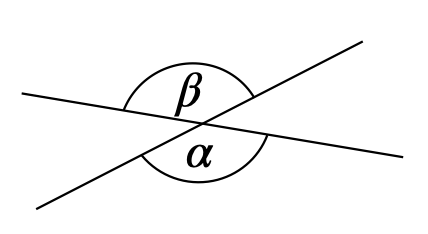
\includegraphics{pictures/7-Scheitelwinkel.png} & \(\alpha = \beta\) \\
  Nebenwinkelsatz & \(\alpha\) und \(\beta\) sind ein Nebenwinkelpaar. & 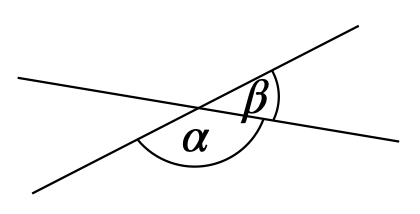
\includegraphics{pictures/7-Nebenwinkel.png} & \(\alpha + \beta = 180°\) \\
  Stufenwinkelsatz & \(\alpha\) und \(\beta\) sind Stufenwinkel an geschnittenen Parallelen. & 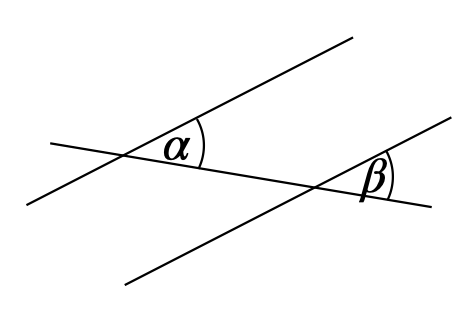
\includegraphics{pictures/7-Stufenwinkel.png} & \(\alpha = \beta\) \\
  Wechselwinkelsatz & \(\alpha\) und \(\beta\) sind Wechselwinkel an geschnittenen Parallelen. & 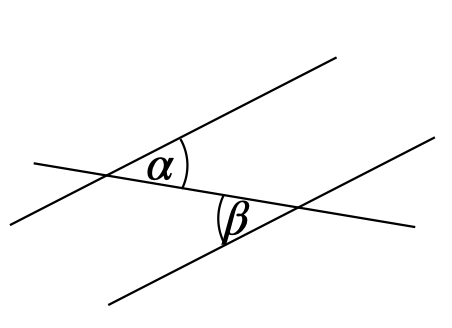
\includegraphics{pictures/7-Wechselwinkel.png} & \(\alpha = \beta\) \\
  \end{longtable}
  \end{quote}
\item
  Ebenfalls der Betonung der inneren Struktur dienlich sind \textbf{strukturbetonende Realisierungsmöglichkeiten}. In diesen wird ein Zusammenhang dargestellt und die Darstellung dient gleichzeitig als »Ausfüllhilfe«. Solche Darstellungen mit Platzhaltern bieten sich insbesondere bei algebraischen Zusammenhängen an.

  \begin{quote}
  Die erste binomische Formel lässt sich in der Form \(({\large\bigcirc} + \boxed{\phantom{X}})^2 = {\large\bigcirc}^2 + 2\cdot {\large\bigcirc}\cdot \boxed{\phantom{X}} + \boxed{\phantom{X}}^2\) darstellen, wobei die Kreise und Boxen mit entsprechenden Werten oder Variablen gefüllt werden können.
  \end{quote}
\item
  Für das \emph{Finden einer Begründung} kann folgende \textbf{Handlungsvorschrift} als Orientierungshilfe dienen (angelehnt an \citeproc{ref-Steinhofel1988}{Steinhöfel et al., 1988, S. 72}):

  \begin{enumerate}
  \def\labelenumi{\arabic{enumi}.}
  \tightlist
  \item
    Formulieren des Zusammenhangs als \textbf{Wenn-dann-Aussage}
  \item
    Feststellen von \textbf{Voraussetzung und Behauptung}
  \item
    Erstellen einer \textbf{Überlegungsfigur}, Bezeichnung wichtiger Teile sowie der Voraussetzung und Behauptung
  \item
    \textbf{Überlegung, woraus die Behauptung folgen} kann. Dabei Verwendung der Überlegungsfigur sowie Orientierung an

    \begin{itemize}
    \tightlist
    \item
      Definitionen vorkommender Begriffe
    \item
      Sätzen mit gleicher Behauptung
    \item
      Sätzen mit ähnlicher Behauptung
    \end{itemize}
  \item
    Abwägung, \textbf{welcher Satz bzw. welche Definition geeignet} ist
  \item
    \textbf{Nachweis der Behauptung} aus den bei 5. gewählten Beweismitteln
  \end{enumerate}
\item
  Für die \emph{Darstellung einer Begründung} kann ein \textbf{Beweisschema} Orientierung bieten. So können bspw. Beweise in einer Tabelle dargestellt werden, bestehend aus einer Spalte zum \textbf{Beweisschritt} und einer zur zugehörigen \textbf{Begründung}. Dies ist insbesondere für \emph{direkte} Beweise geeignet, bei denen von der Voraussetzung zur Behauptung geschlossen wird.
\end{itemize}

\subsection{Zusammenhänge festigen}\label{zusammenhuxe4nge-festigen}

Zum Festigen von Zusammenhängen eignet sich nach Steinhöfel et al. (\citeproc{ref-Steinhofel1988}{1988, S. 34}) u.~a. die \textbf{Einschränkung einer oder mehrerer Voraussetzungen} oder das \textbf{Vertauschen von Voraussetzung und Behauptung}, um die weitere Gültigkeit zu prüfen. Wie auch schon bei Begriffen sollten weiterhin \textbf{Bezeichnungen variiert} und \textbf{alternative Formulierungen} betrachtet werden. Auch bietet es sich an, \textbf{Zusammenhänge mit gleicher oder ähnlicher Behauptung} zu betrachten. Auch hier sei an die systematische Übersicht in Tabelle \ref{tab:festigen} verwiesen.

Nach Vollrath \& Roth (\citeproc{ref-Vollrath2012}{2012, S. 49}) ist ein Zusammenhang verstanden, wenn Schülerinnen und Schüler

\begin{itemize}
\tightlist
\item
  den Zusammenhang angemessen formulieren können,\\
\item
  Beispiele für den Zusammenhang angeben können,\\
\item
  wissen, unter welchen Voraussetzungen der Zusammenhang gilt,\\
\item
  den Zusammenhang begründen können,\\
\item
  Konsequenzen des Zusammenhangs kennen,\\
\item
  Anwendungen des Zusammenhangs kennen.
\end{itemize}

\section{Verfahren}\label{verfahren}

Verfahren dienen in der Mathematik der Verallgemeinerung einer \textbf{Lösung} von einem spezifischen Problem hin zu \textbf{einer ganzen Klasse von Problemen}. Für die ausführenden Schülerinnen und Schüler verschiebt sich damit der (idealerweise) \emph{kreative} Prozess bei der Behandlung von Begriffen und Zusammenhängen hin zu einem \emph{disziplinierten} Arbeiten (vgl. \citeproc{ref-Vollrath2012}{Vollrath \& Roth, 2012, 262~f.}). Dabei darf das Verfahren jedoch nicht als geistig leeres Abarbeiten eines Lösungschemas verstanden werden, sondern auch die »Herkunft des Verfahrens« (z.~B. Begründung einzelner Schritte) sind Bestandteil der Verfahrenskenntnisse.

Vollrath \& Roth (\citeproc{ref-Vollrath2012}{2012, S. 261}, Hervorhebungen im Original) zufolge beziehen sich Verfahren »in der \emph{Arithmetik} in erster Linie auf die Rechenoperationen in den verschiedenen Zahlbereichen, auf das Lösen von Sachaufgaben für Größen mit Hilfe von Funktionen sowie auf die Bestimmung von Funktionswerten; in der \emph{Algebra} betreffen sie das Lösen von Gleichungen, Gleichungssystemen und Ungleichungen; in der \emph{Geometrie} geht es um das Konstruieren, das Berechnen von Umfängen, Flächeninhalten und Rauminhalten, das Darstellen von Körpern und in der \emph{Trigonometrie} um die Dreiecksberechnungen.«

Dabei \textbf{bauen Verfahren auf Begriffe und Zusammenhänge auf} -- benötigen i.~d.~R. sogar mehrere von ihnen. Diese müssen also sicher zur Verfügung stehen. Oftmals ist eine Hierarchie von Begriffen und Zusammenhängen bzw. vorheriger Verfahren nötig, um neue Verfahren aufzubauen (z.~B. baut die schriftliche Multiplikation u.~a. auf die schriftliche Addition und das kleine Einmaleins im Kopf auf, vgl. \citeproc{ref-Vollrath2012}{Vollrath \& Roth, 2012, S. 262}). Die Behandlung von Verfahren dient damit gleichzeitig auch der vertiefenden Aneignung von Begriffen und Zusammenhängen.

\subsection{Verfahren gewinnen}\label{verfahren-gewinnen}

Entsprechend ihrer Eigenschaft, dass Verfahren dem effektiven Lösen einer Klasse von Problemen dienlich sind, können Verfahren über eine \textbf{reflektierende Betrachtung der Lösung spezifischer Probleme derselben Problemklasse} erarbeitet werden. Geeignete Reflexionsfragen sind dabei:

\begin{itemize}
\tightlist
\item
  Was haben all die betrachteten Probleme gemeinsam?
\item
  Welche Schritte haben wir jeweils durchgeführt, um das Problem zu lösen?
\item
  Wozu haben wir die Schritte durchgeführt?
\item
  Warum war es möglich, die Schritte durchzuführen?
\end{itemize}

Die letzten beiden Fragen beziehen sich auf das \emph{Ziel} (»Wozu?«) und den \emph{Weg} (»Warum?«) der jeweiligen Verfahrensschritte.\footnote{Vollrath \& Roth (\citeproc{ref-Vollrath2012}{2012, S. 264}) verweisen hier auf die umgangssprachliche Vermischung der beiden Fragen »Wozu?« und »Warum?«.} Vollrath \& Roth (\citeproc{ref-Vollrath2012}{2012, S. 264}) stellen am Beispiel des Lösens der Gleichung \(5x = 10\) dar, dass eine Unterscheidung zwischen Ziel (»die \(5\) auf die andere Seite bekommen«) und Weg (durch \(5\) dividieren) bei der Verfahrensgewinnung hilfreich sein kann. Während das Ziel die \emph{Notwendigkeit} des Schrittes begründet, nimmt der Weg Bezüge auf die im Hintergrund wirkenden Begriffe und Sachverhalte und liefert damit eine \emph{kausale Begründung} für den Verfahrensschritt.

\subsection{Verfahren aneignen}\label{verfahren-aneignen}

Die Aneignung eines Verfahrens erfolgt i.~d.~R. über dessen Anwendung. Im Sinne der etappenweisen Ausbildung bedeutet dies (\citeproc{ref-Steinhofel1988}{Steinhöfel et al., 1988, S. 118}):

\begin{itemize}
\tightlist
\item
  Auf der \textbf{Etappe der materiellen/materialisierten Handlung} liegt der Verfahrensablauf in schriftlicher Form vor.
\item
  Auf der \textbf{Etappe der sprachlichen Handlung} liegt der Verfahrensablauf nicht mehr schriftlich vor. Die einzelnen Schritte werden von den Schülerinnen und Schülern während der Ausführung kommentiert.
\item
  Auf der \textbf{Etappe der geistigen Handlung} führen die Schülerinnen und Schüler das Verfahren selbstständig und ohne schriftlich vorliegenden Verfahrensablauf aus.
\end{itemize}

Als \textbf{Orientierungshilfe} dient die schriftliche Fixierung des Verfahrensablaufs selbst -- als Wortvorschrift, als Flussdiagramm bzw. als Graph o.~Ä.

\subsection{Verfahren festigen}\label{verfahren-festigen}

Verfahren können u.~a. gefestigt werden, indem einzelne im Verfahren auftretende \textbf{Operanden spezialisiert} werden (z.~B. die beiden Summanden bei der schriftlichen Addition) -- dies entspricht im Endeffekt einer Fallunterscheidung. Auch ist die Untersuchung \textbf{unterschiedlicher Reihenfolgen der Verfahrensoperationen} oder eine \textbf{Variabilität der Darstellung des Verfahrens} (z.~B. Blockschema, Wortvorschrift, Graph, \ldots) möglich. Weiterhin können \textbf{Unter- bzw. Oberalgorithmen} betrachtet, \textbf{Umkehroperationen gebildet} oder \textbf{unterschiedliche Variablengrundbereiche} untersucht werden (vgl. \citeproc{ref-Steinhofel1988}{Steinhöfel et al., 1988, S. 34}).

Nach Vollrath \& Roth (\citeproc{ref-Vollrath2012}{2012, 49~f.}) ist ein Verfahren verstanden, wenn Schülerinnen und Schüler

\begin{itemize}
\tightlist
\item
  wissen, was man damit erreicht,\\
\item
  wissen, wie es geht,\\
\item
  es auf Beispiele anwenden können,\\
\item
  wissen, unter welchen Voraussetzungen es funktioniert,\\
\item
  wissen, warum es funktioniert.
\end{itemize}

\section{Zusammenfassung}\label{zusammenfassung}

In den letzten Abschnitten hat sich gezeigt, dass die Behandlung von Begriffen, Zusammenhängen und Verfahren grundsätzliche Ähnlichkeiten aufweisen. So konnten stets die Teilprozesse einer \textbf{Erarbeitung} (Begriffe bilden, Zusammenhänge und ihre Begründungen finden, Verfahren gewinnen), einer \textbf{Aneignung} (unter Zuhilfenahme von Orientierungshilfen mit dem Ziel der etappenweie Ausbildung geistiger Handlungen) und einer \textbf{Festigung} identifiziert werden. Für letztere zeigt Tabelle \ref{tab:festigen} noch einmal eine Gegenüberstellung von Möglichkeiten.

\begin{longtable}[]{@{}
  >{\raggedright\arraybackslash}p{(\columnwidth - 6\tabcolsep) * \real{0.2500}}
  >{\raggedright\arraybackslash}p{(\columnwidth - 6\tabcolsep) * \real{0.2500}}
  >{\raggedright\arraybackslash}p{(\columnwidth - 6\tabcolsep) * \real{0.2500}}
  >{\raggedright\arraybackslash}p{(\columnwidth - 6\tabcolsep) * \real{0.2500}}@{}}
\caption{\label{tab:festigen} Möglichkeiten zur Festigung von Begriffen, Zusammenhängen und Verfahren, nach Steinhöfel et al. (\citeproc{ref-Steinhofel1988}{1988, S. 34})}\tabularnewline
\toprule\noalign{}
\begin{minipage}[b]{\linewidth}\raggedright
\end{minipage} & \begin{minipage}[b]{\linewidth}\raggedright
Begriffe
\end{minipage} & \begin{minipage}[b]{\linewidth}\raggedright
Zusammenhänge
\end{minipage} & \begin{minipage}[b]{\linewidth}\raggedright
Verfahren
\end{minipage} \\
\midrule\noalign{}
\endfirsthead
\toprule\noalign{}
\begin{minipage}[b]{\linewidth}\raggedright
\end{minipage} & \begin{minipage}[b]{\linewidth}\raggedright
Begriffe
\end{minipage} & \begin{minipage}[b]{\linewidth}\raggedright
Zusammenhänge
\end{minipage} & \begin{minipage}[b]{\linewidth}\raggedright
Verfahren
\end{minipage} \\
\midrule\noalign{}
\endhead
\bottomrule\noalign{}
\endlastfoot
\textbf{Verwendung von Spezial- und Extremfällen} & Unterbegriffe;Grenzfälle & Einschränkung einer oder mehrerer Voraussetzungen im Gültigkeitsbereich; Fallunterscheidungen & Spezialisierung von Operanden (Fallunterscheidungen) \\
\textbf{Umformulieren} & verschiedene Definitionsarten;Definition in Merkmalssystem verwandeln & verschiedene logisch gleichwertige Formulierungen & evtl. unterschiedliche Reihenfolge der Operationen \\
\textbf{Verwendung unterschiedlicher Bezeichnungen} & Merkmale nicht an feste Variablensymbole binden & Voraussetzungen und Behauptungen nicht an feste Symbole binden & unterschiedliche Formalisierungen (Blockschema, Wortvorschrift, Graph, \ldots) \\
\textbf{Bekanntes Neuem gegenüberstellen und Zusammenhänge erkennen lassen} & Oberbegriffe; Einordnung in Begriffssystem & Sätze mit gleicher Behauptung; Sätze mit ähnlicher Behauptung & Unteralgorithmen; Oberalgorithmen \\
\textbf{Umkehrungen bilden} & & Voraussetzungen und Behauptungen vertauschen & Umkehroperationen bilden \\
\textbf{Bedingungen variieren} & Merkmalsvariation durch Weglassen bzw. Hinzufügen von Merkmalen, Ändern der log. Verknüpfung & Weglassen bzw. Hinzufügen von Voraussetzungen & unterschiedliche Variablengrundbereiche \\
\end{longtable}

Weiterführende Möglichkeiten zur Erarbeitung von Begriffen, Zusammenhängen und Verfahren stellen Vollrath \& Roth (\citeproc{ref-Vollrath2012}{2012, 227~ff.}) dar.

\section{Zum Nachbereiten}\label{begriffe-Zusammenhaenge-verfahren-nachbereitung}

\begin{enumerate}
\def\labelenumi{\arabic{enumi}.}
\item
  Beschreiben Sie für ein Verfahren aus der Sekundarstufe I unterrichtliche Möglichkeiten, dieses zu gewinnen.
\item
  Entwickeln Sie, entsprechend der Zusammenfassung in Tabelle \ref{tab:festigen}, Festigungsaufgaben zum Begriff \emph{Erwartungswert}, zum Zusammenhang \emph{Satz des Pythagoras} oder zum Verfahren \emph{Polynomdivision}.
\end{enumerate}

\chapter{Arbeitsmittel}\label{arbeitsmittel}

\begin{quote}
\textbf{Ziele}

\begin{itemize}
\tightlist
\item
  Sie können Arbeitsmittel über Anschaulichkeit, Abstraktheit und Operierbarkeit charakterisieren.
\item
  Sie kennen einen Ablauf zur Ausbildung von Grundvorstellungen mithilfe von Arbeitsmitteln. Dabei sind Sie sich der besonderen Bedeutung des Sprechens über Handlungen bewusst.
\item
  Sie können lerntheoretisch den Einsatz von Arbeitsmitteln bei der Aneignung von Lerngegenständen über Internalisierungs- und Externalisierungsprozesse erläutern.
\end{itemize}

\textbf{Material}

\begin{itemize}
\tightlist
\item
  Folien zum Kapitel 8 (\href{files/Stoffdidaktik2024-08-Arbeitsmittel.pdf}{pdf}, \href{files/Stoffdidaktik2024-08-Arbeitsmittel.key}{Keynote})
\end{itemize}
\end{quote}

Einer der Aspekte der Grundvorstellungsidee ist die Sinnkonstituierung durch Handlungsbezug (siehe Definition \ref{def:Grundvorstellungen}). Sollen Grundvorstellungen bei Schülerinnen und Schülern ausgebildet werden, ist es notwendig, diese Handlungen zu \emph{verinnerlichen} (vgl. Abschnitt \ref{aneignung-von-lerngegenstaenden}). Besonders hilfreich hat sich hierfür der Einsatz von \textbf{Arbeitsmitteln} herausgestellt, anhand derer gehandelt wird.

\section{Begriffsklärung Arbeitsmittel}\label{arbeitsmittel-begriffsklaerung}

In Abschnitt \ref{vermittelnde-werkzeuge} wurde bereits beschrieben, dass in der Tätigkeitstheorie \emph{vermittelnde Werkzeuge} bedeutsam sind in der Auseinandersetzung eines Individuums mit einem Lerngegenstand. Derartige \textbf{\emph{Lernmittel}} können, wie im entsprechenden Abschnitt beschrieben, vielfältiger Natur sein (z.~B. Zirkel und Lineal als Hilfsmittel, Gesten, Sprache, Abbildungen und Skizzen, \ldots{} ).

Als ein spezifisches Lernmittel dient in der Tätigkeitstheorie das Konzept des \textbf{\emph{Lernmodells}}. Lernmodelle sind »sinnliche Stützen geistigen Handelns« (\citeproc{ref-Giest2006}{Giest \& Lompscher, 2006, S. 225}) und können bspw. Zeichnungen, strukturierte Darstellungen, digitale Anwendungen usw. sein. Sie haben als Modelle dabei den Vorteil, dass sie »nicht die konkreten Merkmale der einzelnen Erscheinungen oder Situationen, sondern nur konstitutive, im gegebenen Kontext wesentliche Merkmale und Relationen enthalten, also \emph{abstrakt} sind« (\citeproc{ref-Lompscher1985a}{Lompscher, 1983, S. 64}, Hervorhebung im Original). Gleichzeitig sind sie aber auch »\emph{anschauliche} Abbildungen und machen damit die grundlegenden Zusammenhänge und Wesensmerkmale der Wahrnehmung und Vorstellung zugänglich« (\citeproc{ref-Lompscher1985a}{Lompscher, 1983, S. 64}, Hervorhebung im Original).

\begin{figure}

{\centering 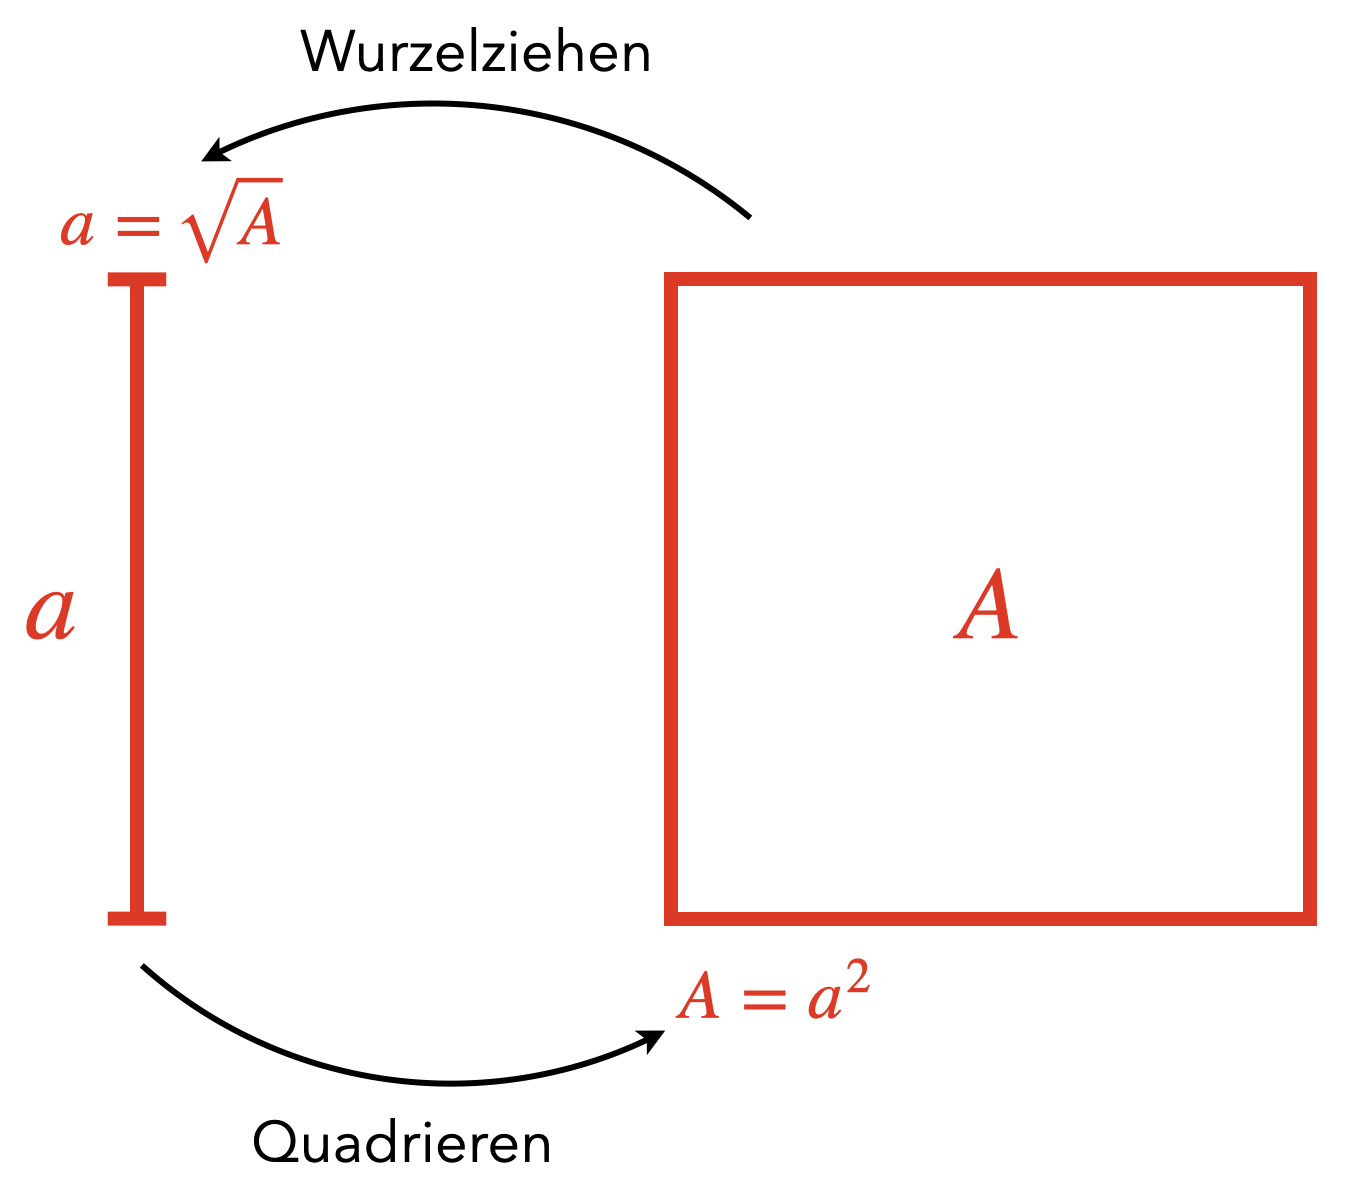
\includegraphics[width=0.25\linewidth]{pictures/8-Lernmodell} 

}

\caption{Beispiel eines Lernmodells für die Bestandteile eines Algorithmus}\label{fig:LernmodellAlgorithmus}
\end{figure}

Lernmodelle können daher insbesondere für mathematische Lerngegenstände dienlich sein, da sie die »abstrakte Struktur des Gegenstands zusammen mit dem prinzipiellen Weg {[}..{]}, der zur Aufdeckung der Struktur geführt hat«, beinhalten (\citeproc{ref-Lompscher1996}{Lompscher, 1996, S. 6}). Dass es sich dabei nicht ausschließlich um Abbildungen, sondern eben auch haptische Materialien oder digitale Anwendungen handeln kann, machen die obigen und noch folgenden Beispiele deutlich.

Die Begriffe \emph{Lernmittel} und \emph{Lernmodell} als tätigkeitstheoretisch geprägte Konzepte werden in der aktuellen Mathematikdidaktik kaum verwendet. Verbreiteter ist dagegen der Begriff des \textbf{Arbeitsmittels}. Nach Krauthausen (\citeproc{ref-Krauthausen:2018}{2018, S. 310}) sind Arbeitsmittel im Mathematikunterricht Veranschaulichungsmittel (zum Illustrieren oder Visualisieren mathematischer Konzepte) oder Anschauungsmittel (d.~h. »Darstellungen mathematischer Ideen in der Hand der Lernenden {[}\ldots{]} zur (Re-)Konstruktion mathematischen Verstehens«). Entscheidend ist hierbei eine »aktivistische« Sichtweise, also dass die Schülerinnen und Schüler die Arbeitsmittel aktiv als »Denkwerkzeug« verwenden. Die Aufgabe der Lehrkraft ist es dabei, »in den sachgerechten Gebrauch ein{[}zu{]}führen und Hilfen (zur Selbsthilfe) im Umgang mit Anschauungsmitteln {[}zu{]} gewähren« (\citeproc{ref-Krauthausen:2018}{Krauthausen, 2018, S. 310}). Reinhold et al. (\citeproc{ref-Reinhold2023}{2023, S. 525}) formulieren in inhaltlich ähnlicher Weise: »Arbeitsmittel im Mathematikunterricht repräsentieren mathematische Objekte und erlauben Handlungen mit den dargestellten Objekten.«\footnote{Den Arbeitsmitteln werden hier \emph{Anschauungsmittel} entgegengestellt, jedoch in einer eher demonstrierenden Bedeutung (\citeproc{ref-Reinhold2023}{Reinhold et al., 2023, S. 526}), was eher dem Begriff der \emph{Veranschaulichungsmittel} bei Krauthausen (\citeproc{ref-Krauthausen:2018}{2018, S. 310}) entspricht.}

In dieser Einordnung übernehmen Arbeitsmittel demnach die Aufgabe eines Lernmittels (auch wenn es weitere Lernmittel gibt, die keine Arbeitsmittel sind). In der obigen Aufzählung der Beispiele kann die \emph{digitale Stellenwerttafel} als Arbeitsmittel aufgefasst werden.

Als Definition für Arbeitsmittel, die sowohl mathematikdidaktische als auch tätigkeitstheoretische Bezüge aufgreift, wird im Folgenden gewählt:

\begin{definition}[Arbeitsmittel]
\protect\hypertarget{def:Arbeitsmittel}{}\label{def:Arbeitsmittel}

Ein Arbeitsmittel ist eine \textbf{materielle oder materialisierte\footnote{Damit sind auch Abbildungen, Strukturdiagramme oder Apps eingeschlossen.}} sowie durch die Schülerinnen und Schüler \textbf{operierbare Repräsentation} eines Lerngegenstands. Damit muss ein Arbeitsmittel folgende Bedingungen erfüllen:

\begin{itemize}
\tightlist
\item
  Es enthält die dem Wesen des Lerngegenstands entsprechenden Merkmale und Relationen \textbf{(Abstraktheit)}.
\item
  Es macht die dem Lerngegenstand zugrundeliegende Struktur der Wahrnehmung und Vorstellung zugänglich \textbf{(Anschaulichkeit)}.
\item
  Es ermöglicht, Lernhandlungen durchzuführen, die der Aneignung des Wesens des Lerngegenstands dienlich sind \textbf{(Operierbarkeit)}.
\end{itemize}

\end{definition}

Bei der Auswahl (oder Entwicklung) eines Arbeitsmittels ist es für Sie als Lehrkraft daher von besonderer Bedeutung, was der \emph{Kern} des entsprechenden mathematischen Gegenstands ist. Hierfür ist es notwendig, dass also das \textbf{Arbeitsmittel mit der \textcolor{concreteColor}{Kernidee} des Lerngegenstands in Einklang} steht. Bezugnehmend auf die \textbf{\textcolor{semanticColor}{Grundvorstellungsidee}} ermöglicht das Arbeitsmittel nun auch \textbf{operatives Handeln in Bezug auf (visuelle) Repräsentationen} und unterstützt damit auch den zweiten Aspekt von Definiton \ref{def:Grundvorstellungen}.

\section{Beispiel Äquivalenzumformungen}\label{beispiel-uxe4quivalenzumformungen}

Bevor Arbeitsmittel für Äquivalenzumformungen von Gleichungen untersucht werden, ist es zunächst notwendig, auf der \textcolor{formalColor}{formalen} und \textcolor{semanticColor}{semantischen} Ebene zu klären, was Gleichungen sind und was man sich unter diesen vorstellen kann.

\subsection{Der Gleichungsbegriff}\label{der-gleichungsbegriff}

Offensichtlich handelt es sich bei dem Ausdruck \(2+ 3 = 5\) um eine Gleichung. Auch der Ausdruck \(2 + 3 = 8\) stellt eine Gleichung dar -- jedoch eine falsche Aussage. Relevant ist bei beiden Ausdrücken, dass zwei Terme durch ein Gleichheitszeichen miteinander verbunden sind. Über den Wahrheitsgehalt einer solchen Gleichung kann jedoch nicht immer eine Aussage getroffen werden. Betrachtet man etwa \(2x = 14\), so kann es sich dabei um eine wahre Aussage (für \(x=7\)) oder um eine falsche Aussage (für \(x\neq 7\)) handeln. In dem Fall spricht man also von einer \emph{Aussageform}, die erst durch Einsetzen der Variable zu einer Aussage wird.

Zusammenfassend gilt: \textbf{Eine Gleichung ist eine Aussageform, in der zwei Terme \(T_1(x)\) und \(T_2(x)\) durch ein Gleichheitszeichen miteinander verbunden werden: \(T_1(x) = T_2(x)\)} (vgl. \citeproc{ref-Weigand2022}{Weigand et al., 2022, 242~ff.})

Liegt eine Gleichung als Aussageform vor, z.~B. \(\frac{7}{x} = 2\), interessiert in der Regel die Lösung der Gleichung, also \(x = 3,\!5\). Ob eine solche Lösung existiert, hängt jedoch von der \textbf{Grundmenge} ab, in der die Aussageform betrachtet wird. Wird für die Gleichung \(\frac{7}{x} = 2\) als Grundmenge \(\mathbb{Z}\) festgelegt, so ist sie nicht lösbar. Ist dagegen \(\mathbb{Q}\) die Grundmenge, so kann eine Lösung angegeben werden. Die Grundmenge entspricht in der Regel dem zur Verfügung stehenden Zahlbereich. Dagegen beschreibt die \textbf{Definitionsmenge} diejenige Teilmenge der Grundmenge, für die die Aussageform überhaupt definiert ist -- im obigen Fall also \(\mathbb{Z}\backslash\{0\}\). Die Menge aller Lösungen, für die die Ausageform eine wahre Aussage ergibt, wird dann als \textbf{Lösungsmenge} bezeichnet und ist demnach wiederum eine Teilmenge der Definitionsmenge.

Weigand et al. (\citeproc{ref-Weigand2022}{2022, S. 257}) unterscheiden in vier Grundvorstellungen zu Gleichungen:

\begin{itemize}
\tightlist
\item
  \textbf{Operationale Grundvorstellung.} Gleichung als Ausdruck einer Berechnung oder Umformung, z.~B. \(2+3 = 5\) oder \(V = \frac{1}{3}\pi r^2 h\).
\item
  \textbf{Relationale Grundvorstellung.} Gleichung als Anlass, Zahlen oder Terme zu ermitteln, für die beide Seiten der Gleichung denselben Wert besitzen, z.~B. \(2x +1 = 7\).
\item
  \textbf{Funktionale Grundvorstellung.} Gleichung als Ausdruck eines Vergleichs zwischen zwei Funktionstermen, z.~B. \(x+1 = -3x\).
\item
  \textbf{Objekt-Grundvorstellung.} Gleichung als ein Objekt, das charakteristische Eigenschaften hat, z.~B. \(x^2 +y^2 = r^2\) als Kreisgleichung.
\end{itemize}

Innerhalb dieser Grundvorstellungen kann nun das \textbf{Lösen von Gleichungen} unterschiedlich interpretiert werden. In der operationalen Grundvorstellung bietet sich bspw. ein Rückwärtsrechnen an, in der funktionalen Grundvorstellung die Schnittpunktbestimmung in einem Diagramm, in dem beide Terme als Funktionsgraphen dargestellt werden. In der Objekt-Grundvorstellung kann das Überprüfen der Passung von Koordinaten zum (ggf. teilweise) Lösen der Gleichung führen, während sich in der relationalen Grundvorstellung Äquivalenzumformungen anbieten.

Für letzteres ist es zunächst notwendig zu klären, was unter der \emph{Äquivalez von Gleichungen} zu verstehen ist. Einerseits ist dies über eine \textbf{Lösungsmengenäquivalenz} möglich, d.~h. zwei Gleichungen (mit derselben Grundmenge) heißen lösungsmengenäquivalent zueinander, wenn sie dieselbe Lösungsmenge besitzen. Die ist etwa bei den Gleichungen \(2x+ 1 = 7\) und \(2x + 3 = 9\) offensichtlich mit der Lösungmenge \(\{3\}\). Jedoch besitzen auch die Gleichungen \(|\mathrm{e}^{\mathrm{i}x}| = 1\) und \(\sin(x) = 0\) dieselbe Lösungsmenge, obwohl die beiden Gleichungen nicht durch offensichtliche Umformungen ineinander übergeführt werden können. Es bietet sich daher auch an, eine \textbf{Umformungsäquivalenz} zu definieren, von der man spricht, wenn zwei Gleichungen durch \textbf{\emph{Äquivalenzumformungen}} ineinander übergeführt werden können. Letztere wiederum ergeben sich, wenn auf beide Seiten der Gleichungen eine eineindeutige, also injektive Funktion angewandt wird, da diese nicht die Lösungsmenge der Gleichung ändert.\footnote{Dies folgt aus folgender Überlegung:Sei eine Gleichung \(T_1(x) = T_2(x)\) mit der Grundmenge \(\mathbb{G}\) gegeben, \(\mathbb{L}\) die Lösungsmenge der Gleichung und \(\varphi: \mathbb{G}\rightarrow \mathbb{G}\) eine injektive Funktion. Für \(x \in \mathbb{L}\) ist \(T_1(x) = T_2(x)\) eine wahre Aussage und damit \(\varphi(T_1(x)) = \varphi(T_2(x))\), also \(x\in\mathbb{L}_\varphi\), d.~h. Lösung der umgeformten Gleichung. Sei weiterhin \(y\in \mathbb{L}_\varphi\), d.~h. \(\varphi(T_1(y)) = \varphi(T_2(y))\). Dann ist wegen der Injektivität \(\varphi^{-1}(\varphi(T_1(y))) = \varphi^{-1}(\varphi(T_2(y)))\), also \(T_1(y) = T_2(y)\), also \(y\in\mathbb{L}\). Daraus folgt \(\mathbb{L} = \mathbb{L}_\varphi\).} Dabei sind die Addition, Subtraktion, Multiplikation und Division (bis auf Division durch Null) derartige injektive Funktionen, also Äquivalenzumformungen. Das Quadrieren einer Gleichung dagegen erhält im Allgemeinen nicht die Lösungsmenge, da die Funktion \(^2: x \mapsto x^2\) nicht injektiv ist.

\subsection{Umformungen verstehen}\label{umformungen-verstehen}

Um Äquivalenzumformungen nachvollziehen zu können, haben sich für den Mathematikunterricht verschiedene Unterstützungsinstrumente etabliert. Diese sollen nun kurz vorgestellt und hinsichtlich ihrer Eignung als Arbeitsmittel (also inwiefern sie die Kriterien aus Definiton \ref{def:Arbeitsmittel} erfüllen) untersucht werden. Die folgenden Betrachtungen beziehen sich ausschließlich auf lineare Gleichungen mit einer Variablen.

\subsubsection{Waage-Modell}\label{waage-modell}

Im Waage-Modell werden Gleichungen über Massestücke auf einer Balkenwaage dargestellt, wobei i.~d.~R. absolute Werte in anderer Größe oder Form dargestellt werden als die Variable. Die Gleichheit wird visualisiert über das Gleichgewicht der Waage, also dass deren Balken horizontal ausgerichtet ist.

Eine Äquivalenzumformung besteht nun darin, in beiden Waagschalen dieselbe Operation durchzuführen, so dass die Waage stets im Gleichgewicht bleibt.

\begin{figure}

{\centering 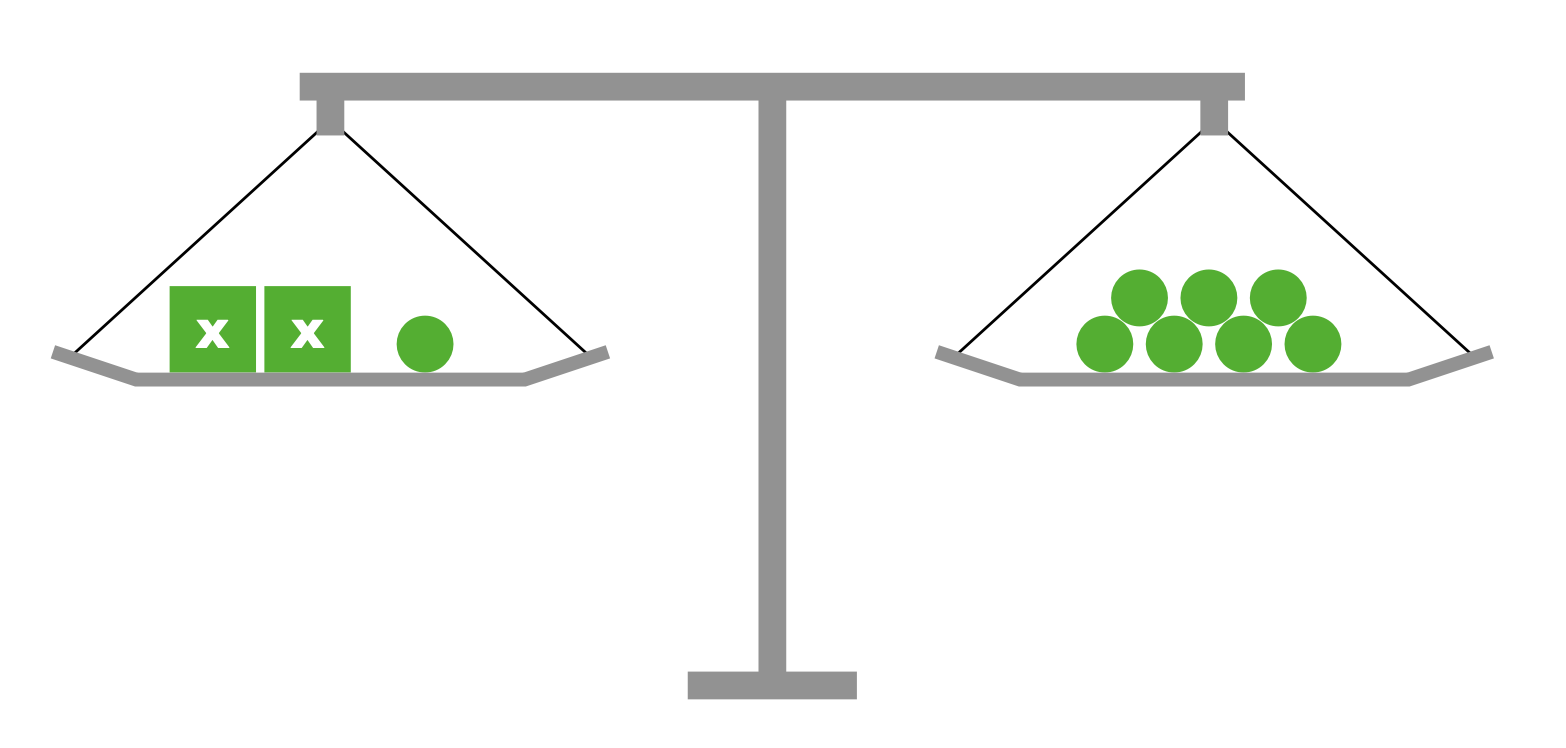
\includegraphics[width=0.75\linewidth]{pictures/8-Waage} 

}

\caption{Waage-Modell für die Gleichung $2x+1 = 7$}\label{fig:Waage}
\end{figure}

Ein Vorteil besteht in der hohen \textbf{Anschaulichkeit} des Modells. Auch die \textbf{Operierbarkeit} ist für Gleichungen mit natürlichen Vorfaktoren und ausschließlich Summen gegeben. Hier zeigen sich aber auch schon erste Schwächen. Nach Weigand et al. (\citeproc{ref-Weigand2022}{2022, 260~f.}) bestehen folgende weitere Hürden und Herausforderungen:

\begin{itemize}
\item
  Negative Zahlen können kaum sinnvoll dargestellt werden. Hier gäbe es etwa die Möglichkeit, dass z.~B. \(x-1\) als ein Massestück für \(x\) mit einem Loch der Größe \(1\) dargestellt wird. Auch ermöglichen digitale Umsetzungen, dass negative Werte eine Bewegung der Waage entgegen der Schwerkraft bewirken. So kann aber nicht mehr an die Handlungserfahrungen mit echten Balkenwaagen angeknüpft werden, in denen das Modell eigentlich seinen Ursprung hat.
\item
  Gleichzeitig muss auch zugegeben werden, dass nur noch wenige Schülerinnen und Schüler tatsächlich Erfahrungen mit Balkenwaagen haben. Der Waagetyp ist einerseits unüblich, andererseits auch sehr empfindlich gegenüber kleinen Masseabweichungen. Es ist also in der praktischen Ausführung recht kompliziert, ein Gleichgewicht herzustellen. Außerdem muss, damit das Gleichgewicht jederzeit bestehen bleibt, auf beiden Seiten gleichzeitig operiert werden.
\item
  Um die Ausgangssituation der gleichgewichteten Waage herzustellen, muss bereits bekannt sein, über welche Masse das \(x\) repräsentierende Massestück verfügt. Wird also die Situation nicht vorgegeben, erscheint das Lösen unnötig. Außerdem bestünde in der Realität die Möglichkeit, durch Versuch und Irrtum die Masse von \(x\) mit der Waage zu bestimmen, so dass Äquivalenzumformungen ggf. nicht notwendig erschienen und das Vorgehen noch nicht einmal dem Einsetzen verschiedener Werte für \(x\) in die Gleichung entspräche (was einem innermathematischen Versuchen entspräche).
\item
  Hinzu kommt, dass das Dividieren zunächst mit einem Bündeln und dann einem Wegnehmen einhergeht. Dies weist (in der äußeren Handlung) Ähnlichkeiten zum Subtrahieren auf, was es jedoch nicht ist.
\end{itemize}

All diese Einschränkungen und mögliche »Reparaturen« des Modells bzw. des Umgangs mit ihm lassen darauf deuten, dass die \textbf{Abstraktheit} des Modells zu gering ist, es also nicht in ausreichendem Maße das Wesen des Lerngegenstand darstellen kann. Der Drang, nicht mögliche Operationen in das anschauliche Modell zu »pressen«, spricht dafür, dass das Modell auf mathematischer Ebene nicht geeignet genug erscheint, um die Anforderungen an die obige Arbeitsmittel-Definition zu erfüllen.

Dies soll jedoch nicht bedeuten, dass das Modell keinesfalls genutzt werden darf. Barzel \& Holzäpfel (\citeproc{ref-Barzel2011a}{2011, S. 7}) empfehlen, »das Waage-Modell für den Einsatz mit natürlichen Zahlen auf jeden Fall zu nutzen, um das Prinzip der Äquivalenzumformungen zu erläutern.« Dabei sollten die Grenzen des Modell deutlich gemacht werden und anschließend entweder innermathematisch oder mit alternativen Modellen weitergearbeitet werden.

\subsubsection{Streichholzschachtel-Modell}\label{streichholzschachtel-modell}

Eine weitere Möglichkeit bietet das Streichholzschachtel-Modell, bei denen \(x\) die Anzahl der Streichhölzer in einer Schachtel beschreibt, die Gleichung entsprechend mit Schachteln und einzelnen Streichhölzern dargestellt und dann ähnlich wie beim Waage-Modell über gleichartiges Operieren auf beiden Seiten gelöst wird.

\begin{figure}

{\centering 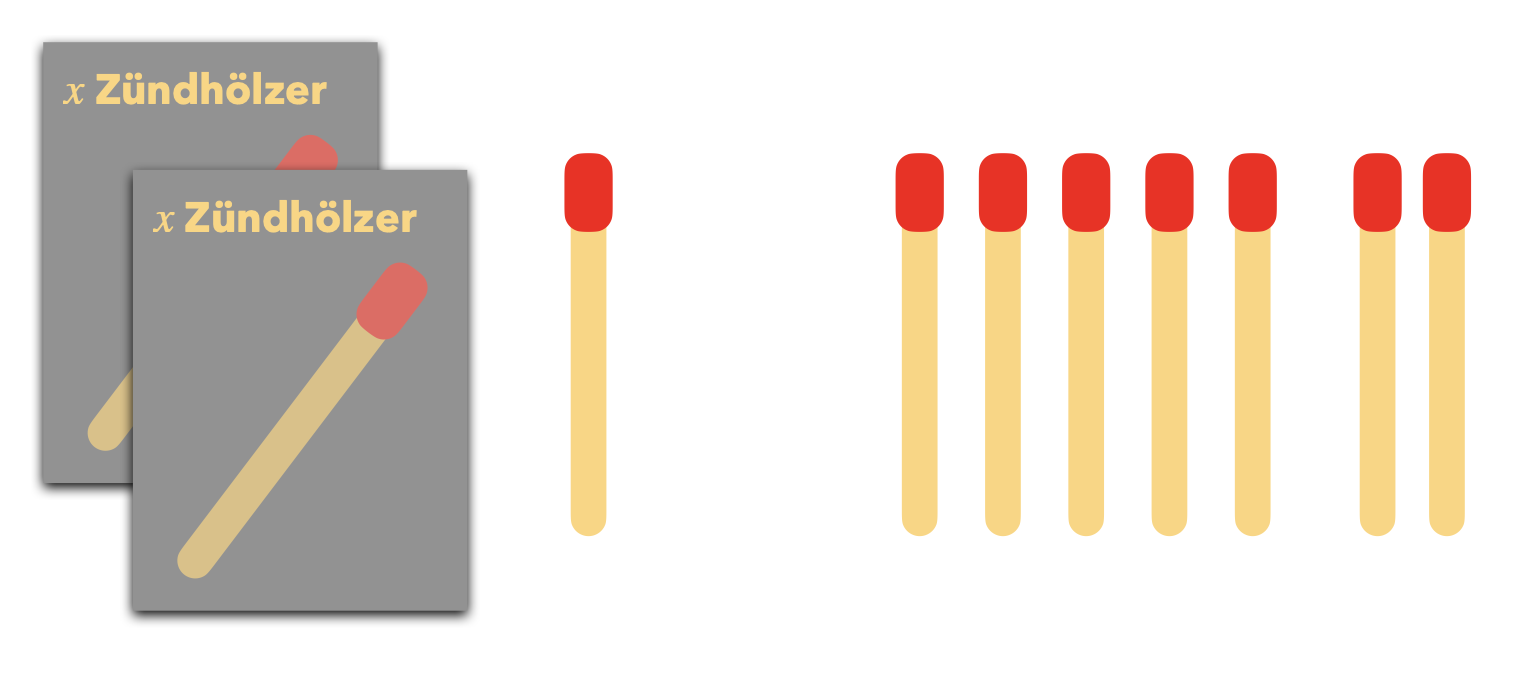
\includegraphics[width=0.75\linewidth]{pictures/8-Streichholz} 

}

\caption{Streichholzschachtel-Modell für die Gleichung $2x+1 = 7$}\label{fig:Streichholz}
\end{figure}

Gegenüber dem Waage-Modell bietet dieses Modell eine einfachere Zugänglichkeit (v.~a. in der tatsächlichen Unterrichtssituation) und die Anzahl der Hölzer pro Schachtel ist tatsächlich unbekannt. Jedoch muss man einerseits darauf vertrauen, dass in allen Schachteln dieselbe Anzahl an Streichhölzern vorhanden ist und auch die Gleichheit beider Seiten kann nicht (wie z.~B. durch die ausgeglichene Waage) visualisiert werden. In dem Sinne ist die \textbf{Anschaulichkeit} etwas geringer, die \textbf{Operierbarkeit} für die Schülerinnen und Schüler etwas besser als beim Waage-Modell.

Hinsichtlich der \textbf{Abstraktheit} sind keine Unterschiede zu verzeichnen: Es ist weiterhin nur eine Bearbeitung mit natürlichen Vorfaktoren und Variablen sinnvoll möglich.

Barzel \& Holzäpfel (\citeproc{ref-Barzel2011a}{2011, S. 6}) betonen, dass Streichholzschachteln, Plättchen oder Dosen bereits beim Aufstellen von Termen geeignete Visualisierungsinstrumente sind. Insofern bietet dieses Modell eine gute Anschlussfähigkeit zu vorherigen Erfahren.

\subsubsection{Strecken-/Pfeil-Modell}\label{strecken-pfeil-modell}

Weigand et al. (\citeproc{ref-Weigand2022}{2022, 261~f.}) beschreibt ein Modell, in dem die beiden Terme einer Gleichung über zwei Strecken dargestellt werden, jeweils zusammengesetzt aus Repräsentanten für die Variablen und für die absoluten Werte. Die Gleichheit zeigt sich dann über die gleiche Länge der Strecken. Eine Verallgemeinerung zu Pfeilen ist möglich und wird unten noch diskutiert.

\begin{figure}

{\centering 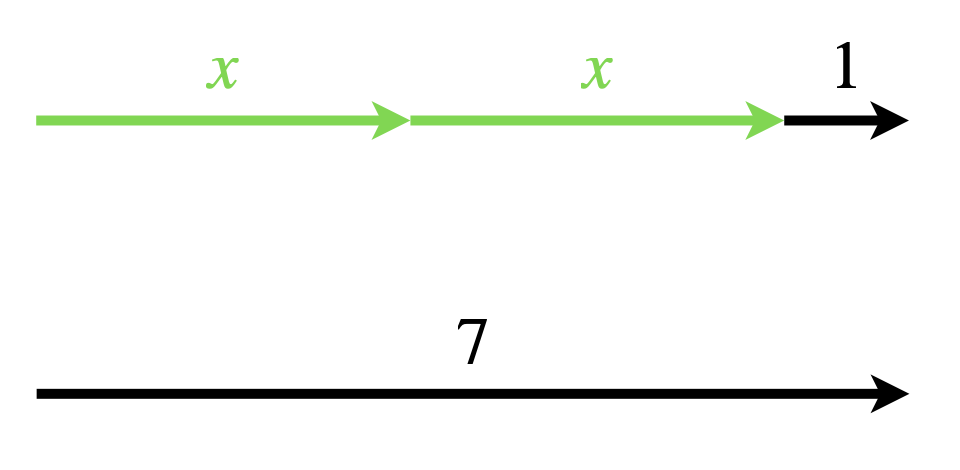
\includegraphics[width=0.5\linewidth]{pictures/8-Pfeile} 

}

\caption{Pfeil-Modell für die Gleichung $2x+1 = 7$}\label{fig:Pfeile}
\end{figure}

Äquivalenzumformungen sind nun über gleichzeitiges Abziehen oder Hinzufügen bzw. Auftrennen von (Teil-)Strecken visualisierbar. Dieses Modell greift offensichtlich nicht auf derart enaktive Erfahrungen zurück, wie es das Waage- oder Streichholzschachtel-Modell tun. Dennoch erfüllt es das Kriterium der \textbf{Anschaulichkeit}, weil es die dem Lerngegenstand zugrundeliegende Struktur der Wahrnehmung und Vorstellung zugänglich macht. Die \textbf{Operierbarkeit} ist für gedankliche Operationen und, wenn die Strecken z.~B. über Papierstreifen realisiert werden, auch in Form von real durchgeführten Operationen möglich. Eine digitale Umsetzung des Modells kann bspw. die Operierbarkeit erhöhen und zu einer virtuell-enaktiven Handlungsoption führen.

Ein großer Vorteil des Modells liegt jedoch in der \textbf{Abstraktheit}:

\begin{itemize}
\item
  So sind gleichermaßen natürliche wie (positive) gebrochenrationale Vorfaktoren visualisierbar, was sich nur in der Länge der (Teil-)Strecken auswirkt.
\item
  Auch negative Vorfaktoren können über Pfeile in die Gegenrichtung repräsentiert werden. Eine solche Darstellung ist im Umgang mit der Zahlengeraden bekannt, kann auch bei Termen wieder aufgegriffen und hier nun zum Lösen von Gleichungen weiter genutzt werden.
\end{itemize}

\begin{figure}

{\centering 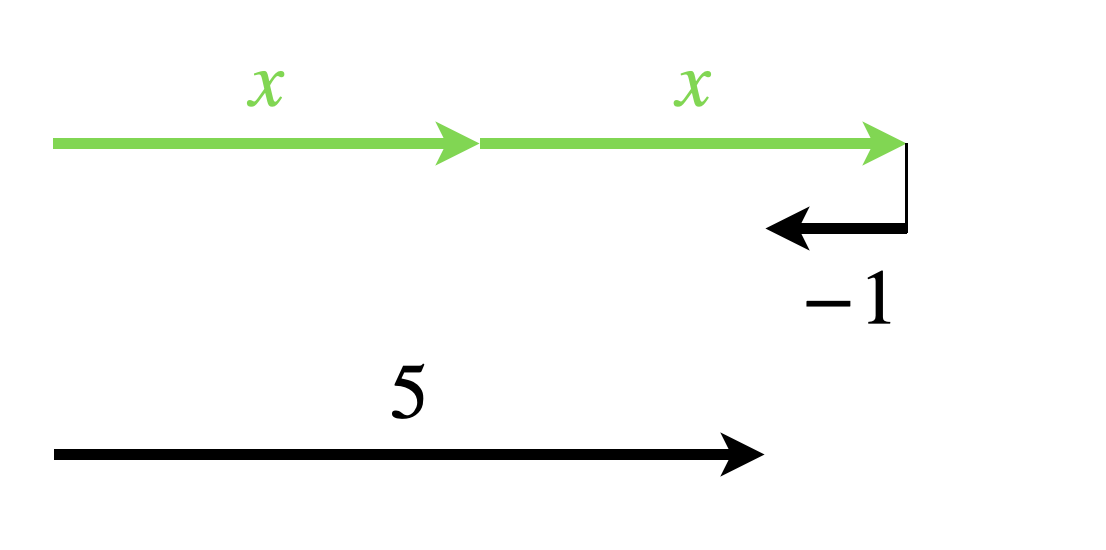
\includegraphics[width=0.5\linewidth]{pictures/8-negativePfeile} 

}

\caption{Pfeil-Modell für die Gleichung $2x-1 = 5$}\label{fig:negativePfeile}
\end{figure}

\begin{itemize}
\tightlist
\item
  Das Modell bietet weiterhin die Möglichkeit, die Gleichheit der beiden Terme abhängig vom Wert für \(x\) nachvollziehbar zu machen. Je nachdem, wie groß \(x\) ist, kann also die Gleichung \(2x+1 = 7\) wahr sein (beide Strecken gleich lang) oder eben nicht. Unterstützt werden kann dies, indem \(x\) dynamisch variiert wird, etwa in einem digitalen Arbeitsmittel.
\end{itemize}

Insofern erfüllt eine Umsetzung dieses Modells über ein digitales Arbeitsmittel, in dem virtuell-enaktiv operiert werden kann, die Forderungen aus Definition \ref{def:Arbeitsmittel}.

\section{Zum Nachbereiten}\label{arbeitsmittel-nachbereitung}

In Kapitel \ref{grundvorstellungen} sollten Sie sich in der Nachbereitung mit Grundvorstellungen zu \emph{Variablen} oder \emph{Termen} beschäftigen.

\begin{enumerate}
\def\labelenumi{\arabic{enumi}.}
\item
  Recherchieren Sie in Schulbüchern und fachdidaktischer Literatur, welche Materialien üblicherweise zur Unterstützung des Aufbaus entsprechender Grundvorstellungen verwendet werden.
\item
  Analysieren Sie eines dieser Materialien hinsichtlich der Eignung als Arbeitsmittel nach Definition \ref{def:Arbeitsmittel}.
\end{enumerate}

\part*{Didaktik der Sachgebiete}\label{part-didaktik-der-sachgebiete}
\addcontentsline{toc}{part}{Didaktik der Sachgebiete}

\chapter{Arithmetik und Algebra}\label{arithmetik-und-algebra}

\begin{quote}
\textbf{Ziele}

\begin{itemize}
\tightlist
\item
  Sie haben einen Überblick, was Arithmetik- und Algebra-Unterricht auszeichnet.\\
\item
  Sie können den Zusammenhang zwischen den Sachgebieten Arithmetik und Algebra und den zugehörigen Leitideen beschreiben.\\
\item
  Sie kennen Verfahren zum näherungsweisen Bestimmen von Quadratwurzeln sowie deren algorithmische Umsetzung.
\end{itemize}

\textbf{Material}

\begin{itemize}
\tightlist
\item
  Folien zum Kapitel 9 (\href{files/Stoffdidaktik2024-09-ArithmetikUndAlgebra.pdf}{pdf}, \href{files/Stoffdidaktik2024-09-ArithmetikUndAlgebra.key}{Keynote})
\end{itemize}

\textbf{Literaturempfehlungen}

\begin{itemize}
\tightlist
\item
  Padberg \& Benz (\citeproc{ref-Padberg2021}{2021}): \emph{Didaktik der Arithmetik: fundiert, vielseitig, praxisnah}
\item
  Weigand et al. (\citeproc{ref-Weigand2022}{2022}): \emph{Didaktik der Algebra: nach der Vorlage von Hans-Joachim Vollrath}
\end{itemize}
\end{quote}

In diesem und den folgenden Kapiteln sollen für die einzelnen Sachgebiete der Mathematik teils einige allgemeine Kommentare zur Didaktik des jeweiligen Sachgebiets getroffen und stets an ausgewählten Lerngegenständen mathematikdidaktische Hintergründe illustriert werden. Die Auswahl der Lerngegenstände erfolgt dabei interessen- und zufallsgesteuert und stellt keine systmatische Betrachtung dar.

\section{Übergang Arithmetik → Algebra}\label{uxfcbergang-arithmetik-algebra}

»In der Arithmetik sind Zahlen die Objekte des Handelns.« Weigand et al. (\citeproc{ref-Weigand2022}{2022, S. 40}) formuliert diesen Satz, um im Kontrast dazu zu beschreiben, dass sich in der Algebra »der Fokus vom Handeln mit Zahlen zum Handeln mit unbekannten Größen {[}verändert{]}. Dabei können Lernende die bekannten Regeln des Operierens mit Zahlen auf die neuartige Situation übertragen, in der Zahlen unbekannt sind.«
Der Mathematikunterricht der Sekundarstufe I ist geprägt durch diesen gedanklichen Übergang von der Arithmetik zur Algebra, der aber durchaus auch schon in der Grundschule beginnen kann, etwa beim halbschriftlichen Rechnen (siehe z.~B. \citeproc{ref-Padberg2021}{Padberg \& Benz, 2021, 191~ff.}). »Aus der Perspektive des Lehrens und Lernens von Algebra beginnt die Auseinandersetzung mit Algebra dort, wo Lernende allgemeine arithmetische Strukturen erkennen oder erkunden« (\citeproc{ref-Weigand2022}{Weigand et al., 2022, S. 39}). Die bedeutsamsten Lerngegenstände zur Algebra sind demnach \textbf{Variablen}, \textbf{Terme} und \textbf{Gleichungen}.

Die Algebra erhält im Schulunterricht drei wesentliche Bedeutungen (Zitate entnommen aus \citeproc{ref-Weigand2022}{Weigand et al., 2022, S. 1~ff.}):

\begin{itemize}
\item
  \textbf{Algebra als Formelsprache.} »Mithilfe von Variablen, Termen und Gleichungen kann ein Sachverhalt in der Formelsprache dargestellt werden.« Dies wird beispielsweise bei der binomischen Formel \((a+b)^2 = a^2+2ab+b^2\) sichtbar, die das Distributivgesetz für einen bestimmten Fall beschreibt.
\item
  \textbf{Algebra als Werkzeug.} Demnach ist die »Algebra ein Hilfsmittel und Werkzeug, um geometrische, physikalische oder Anwendungsprobleme durch Formelsprache auszudrücken und so zu lösen«. So könn etwa die Kosten in Euro für eine Taxifahrt über die Gleichung \(K = 4,4+2,1t\) beschrieben werden, wenn \(t\) die gefahrenen Minuten darstellt.
\item
  \textbf{Algebra als Denkweise.} »Algebraisches Denken zeigt sich somit im Umgang mit Denkobjekten beim Übergang von konkreten zu unbestimmten Objekten und beim Operieren auf der symbolischen Ebene.« Dies kann etwa bei der Betrachtung von Musterfolgen der Fall sein. Neben der Anzahl an Würfeln in den einzelnen Schritten in Abbildung ? könnte das Interesse darauf gelegt werden, wie sich die Anzahl von Schritt zu Schritt verändert und wie viele Würfel dann im \(n\)-ten Schritt vorhanden sind.
\end{itemize}



\begin{figure}

{\centering 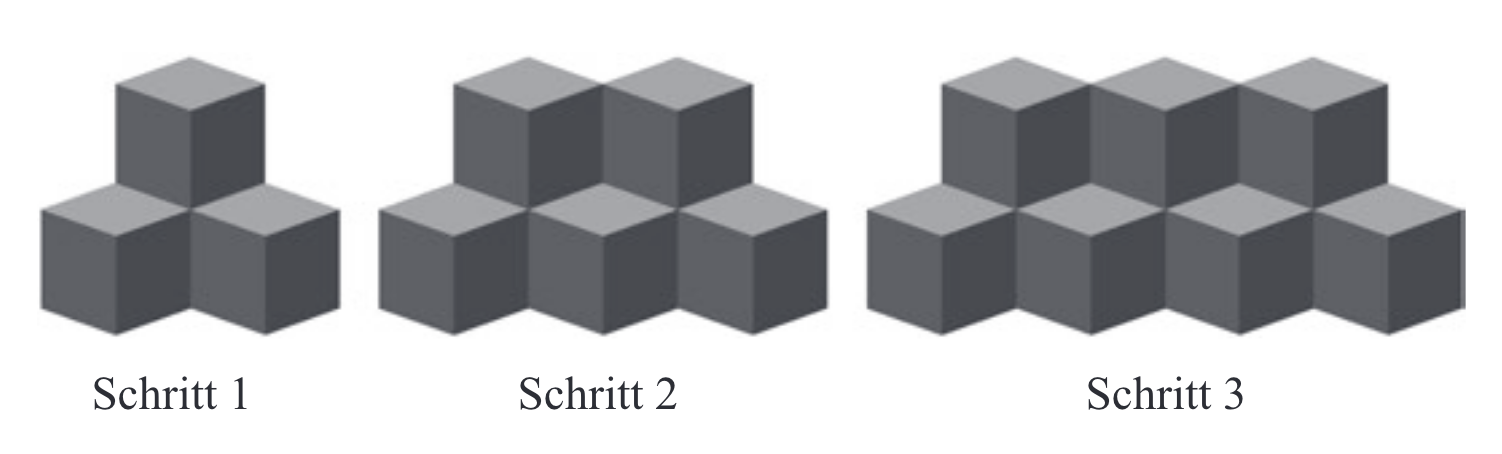
\includegraphics[width=0.75\linewidth]{pictures/9-Musterfolge} 

}

\caption{Musterfolge zum Übergang der Arithmetik zur Algebra (\citeproc{ref-Weigand2022}{Weigand et al., 2022, S. 8})}\label{fig:Musterfolge}
\end{figure}

\section{Wurzeln}\label{wurzeln}

\subsection{Begriffsverständnis}\label{wurzel-begriffsverstaendnis}

In diesem Abschnitt werden \textbf{Begriffsinhalt}, \textbf{Begriffsumfang} und \textbf{Begriffsnetz} sowie verschiedene \textbf{Stufen des Begriffsverständnisses} zum Wurzelbegriff diskutiert\footnote{Mehr zu diesen Begriffen siehe im Kapitel \href{https://stoffdidaktik.heiko-etzold.de/2021/6-begriffsbildung.html}{6.1} des Skripts von 2021/22 zur Stoffdidaktik Mathematik}.

Zunächst ist festzuhalten, dass die Wurzel bzw. das Wurzelziehen die Umkehrung des Quadrierens im Bereich der nichtnegativen Zahlen ist. Diese Nichtnegativität ist übrigens im Unterricht besonders herauszuarbeiten. Während \((-3)^2 = 9\) und \(3^2= 9\) ist, also die Gleichung \(x^2 = 9\) zwei Lösungen in den reellen Zahlen hat, ist \(\sqrt{9} = 3\) eindeutig festgelegt. Man kann also nicht pauschal von der Wurzel als die Umkehrung des Quadrates sprechen.\footnote{Dies wird bei höheren Exponenten sogar noch bedeutsamer: Dort ist \((-3)^3 = -27\). Die Gleichung \(x^3 = -27\) ist im Reellen sogar eindeutig lösbar (im Komplexen dagegen hat sie drei Lösungen), aber \(\sqrt[3]{-27}\) ist nicht definiert. Gerade, weil einige Taschenrechner fälschlicherweise die dritte Wurzel aus \(-27\) mit \(-3\) angeben, muss auf eine derartige Gefahr eingegangen werden, wenn Wurzeln höherer Exponenten behandelt werden. Dies zeigt einmal mehr, dass Sie als Lehrkraft über den aktuellen Unterrichtsstoff (z.~B. Quadratwurzeln) hinausdenken müssen (z.~B. Kubikwurzeln), um Rückschlüsse ziehen zu können, welche inhaltlichen Besonderheiten zu betonen sind.} Weiterhin gehört zum Begriffsinhalt die Eigenschaft, dass Wurzeln nicht immer rational sein müssen, auch wenn die Zahl, aus der die Wurzel gezogen wird, rational ist (z.~B. bei \(\sqrt{2}\)). Der Wert einer Wurzel lässt sich jedoch mittels rationaler Zahlen annähern\footnote{Die fachmathematische Grundlage hierfür ist, dass Cauchy-Folgen in den reellen Zahlen immer konvergieren und sich die nichtnegative Lösung der Gleichung \(x^2 = a\) mit \(a\geq 0\) über eine rationale Cauchy-Folge nähern lässt -- konkret mit dem \emph{Heron-Verfahren}.}. Das Vorgehen zum Finden einer Annäherung kann durchaus auch als Bestandteil des Begriffsinhalts aufgefasst werden.

Wurzeln können demnach alle nichtnegativen reellen Zahlen sein, da für jede (rationale oder reelle) Zahl \(a\geq 0\) eine reelle Zahl \(x\geq 0\) gefunden werden kann, für die \(x^2 = a\) gilt. Dieser Begriffsumfang kann sich jedoch erst schrittweise entwickeln, da mit der Einführung des Wurzelbegriffs in der Regel noch nicht die reellen Zahlen bekannt sind. Die Menge aller Wurzeln rationaler Zahlen besteht zwar aus nichtnegativen reellen Zahlen -- aber noch nicht aus allen (denn z.~B. \(\sqrt{\pi}\) existiert ja auch). Ein vollständiger Begriffsumfang des Wurzelbegriffs ist also erst dann ausgeprägt, wenn die reellen Zahlen eingeführt wurden.

Eng verbunden ist der Wurzelbegriff mit dem des \emph{Quadrates} (sowohl algebraisch als auch geometrisch) und den \emph{reellen Zahlen} (als \emph{Lückenfüller} der rationalen Achse). Auch das \emph{Wurzelziehen} bzw. \emph{Radizieren}\footnote{Hier lohnt es sich übrigens, auf die Wortherkunft einzugehen und zu begründen, warum Radieschen als solche bezeichnet werden.} als verwandte Arbeitsbegriffe gehören zum engen Begriffsnetz. Bei der Betrachtung der Gleichung \(x^2 = a\) sind auch \emph{Basis} und \emph{Exponent} sowie der \emph{Radikant}, v.~a. in der Schreibweise \(\sqrt{a} = x\), Bestandteile des Begriffsnetzes. Der \emph{Wurzelexponent} wird dann v.~a. bei höheren Exponenten von Bedeutung, wenn er in der Schreibweise \(\sqrt[n]{a}\) auftritt. Ob die \emph{Intervallschachtelung} als Fachbegriff im Zusammenhang mit dem Wurzelziehen auftauchen muss, sollte abhängig von der Lerngruppe entschieden werden -- bekommt damit aber eine besondere Bedeutung als Begriff eines Verfahrens.

Hinsichtlich des Wurzelbegriffs liegt ein \emph{intuitive Begriffsverständnis} vor, wenn die Schülerinnen und Schüler Wurzeln als Seitenlängen zu Quadraten mit vorgegebenen Flächeninhalten auffassen oder dies in einer algebraischen Sichtweise nachvollziehen. Zum \emph{inhaltlichen Begriffsverständnis} gehört darauf aufbauend hinzu, dass es sich stets um nichtnegative Werte handeln muss. Ein \emph{integriertes Begriffsverständnis} liegt vor, wenn die Monotonie und nicht-Linearität erkannt ist, also bspw. die näherungsweise Bestimmung einer Wurzel möglich ist. Auch der begriffliche Zusammenhang zu \emph{Quadrat}, \emph{Basis} und \emph{Exponent} kann auf dieser Stufe von den Schülerinnen und Schülern hergestellt werden. Bestandteil der Stufe ist (später) ebenfalls die Verknüpfung zu höheren Potenzen und deren \(n\)-te Wurzeln. Das \emph{formale Begriffsverständnis} geht einher mit der Kenntnis und Anwendbarkeit der Definition der Wurzel, hier insbesondere auch die Fähigkeit zu begründen, warum es keine negativen Wurzeln bzw. keine Wurzeln aus negativen Zahlen gibt.

\subsection{Wurzelbehandlung}\label{wurzelbehandlung}

Angelehnt an die \emph{Mathewerkstatt} für die Klassenstufe 9 (\citeproc{ref-Barzel2016}{Barzel et al., 2016, 92~ff.}) sowie die Überlegungen in den Kapiteln \ref{taetigkeitstheorie-und-lernen} und \ref{begriffe-sachverhalte-und-verfahren}, bietet sich folgende Behandlung des Wurzelbegriffs an:

\begin{enumerate}
\def\labelenumi{\arabic{enumi}.}
\item
  Es kann prinzipiell davon ausgegangen werden, dass den Schülerinnen und Schülern Quadrate bekannt sind und sie aus diesen Seitenlängen abmessen und den Flächeninhalt berechnen können. In Hinblick auf die \emph{Zone der nächsten Entwicklung} sind sie noch nicht in der Lage, aus gegebenen Flächeninhalten die Seitenlänge eines Quadrates zu berechnen bzw. halbquantitive Zusammenhänge zu erzeugen (z.~B. \emph{Wie ändert sich die Seitenlänge, wenn der Flächeninhalt halbiert wird?}). Jedoch können sie diese Anforderungssituation mit ihrem bisherigen Wissen verstehen.

  Der (innermathematische) \textbf{Kontext} ist also das Bestimmen einer Seitenlänge eines Quadrates bei gegebenem Flächeninhalt. Dies kann u.~a. dadurch konkretisiert werden, dass zu einem Quadrat dasjenige mit dem halben Flächeninhalt gesucht wird. Dies erhöht die Konxtauthentizität dahingehend, das es sich um ein historisch relevantes Problem handelt (vgl. \citeproc{ref-Barzel2016}{Barzel et al., 2016, S. 94}). Dabei ist es reichthaltig genug, auch von der Halbierung abzusehen und allgemeinere Zusammenhänge zu erkunden. Ein erster Lösungsversuch ist zum Beispiel über das Falten eines quadratischen Blatt Papiers möglich (indem alle vier Ecken auf den Mittelpunkt gefaltet werden). Durch einen Vergleich des ursprünglichen und des gefalteten Quadrates kann man erkennen, dass die Seitenlänge nicht einfach halbiert werden kann.
\item
  Als \textbf{Lernziel} kann herausgearbeitet und formuliert werden: \emph{Wir wollen für ein Quadrat mit einem bestimmten Flächeninhalt die Seitenlänge bestimmen können.} Dies ist allgemeiner formuliert als das Halbierungsproblem, aber eine solch allgemeine Formulierung ist durchaus sinnvoll, um das übergeordnete Ziel während des Lernprozesses stets vor Augen zu haben. Wichtig ist hierbei, dass auch das Ziel selbst von den Lernenden verstanden wird und sie jederzeit überprüfen können, inwieweit sie das Ziel schon erreicht haben.
\item
  Bei der Überlegung, welche \textbf{Lernhandlungen} geeignet sind, sich dem Wurzelbegriff zu nähern, sollen diese aus den fachlich relevanten Zusammenhängen extrahiert und am gewählten Kontext konkretisiert werden:

  \begin{itemize}
  \item
    Ein wesentlicher Zusammenhang ist, dass sich \textbf{Seitenlänge und Flächeninhalt eines Quadrates nicht proportional zueinander} verhalten, also eine doppelte Seitenlänge nicht zu einem doppelten Flächeninhalt führt. Dieser nicht-Zusammenhang gilt aber dann natürlich auch umkehrt: Der doppelte Flächeninhalt wird nicht durch eine doppelte Seitenlänge verursacht. Diese Perspektive ist wichtig, um zu erkennen, dass sich Wurzeln unbekannter Zahlen nicht so einfach linear aus Wurzeln bekannter Zahlen konstruieren lassen. Als konkrete Lernhandlung lässt sich die umsetzen, indem \textbf{zu vorgegebenen Quadraten Seitenlängen und Flächeninhalte bestimmt werden} müssen. Die Auswahl sollte derart erfolgen, dass sowohl vielfache Seitenlängen als auch vielfache Flächeninhalte auftreten, damit bei den jeweils anderen Größen erkannt wird, dass diese keine entsprechenden Vielfachen darstellen.
  \item
    Trotz der nicht-Linearität ist die bestehende \textbf{(strenge) Monotonie} ein weiterer Zusammenhang \textbf{zwischen Seitenlängen und Flächeninhalt.} Dieser kann herausgearbeitet werden, indem (nach der vorherigen Erfahrung) \textbf{Flächeninhalte und Seitenlängen von Quadraten} gegeben werden und zwischen diesen eine \textbf{Zuordnung} erfolgen muss. Dies betont den qualitativen Zusammenhang -- auch wenn ein konkretes Ausrechnen damit noch nicht möglich ist.
  \item
    Der nächste Handlungsschritt ist nun das \textbf{näherungsweise Bestimmen von Seitenlängen} über das Intervallschachtelungsprinzip. Dieses baut in fachlicher Hinsicht auf die Monotonie auf und es sind nun immer Zahlenpaare \(a_1\) und \(a_2\) gesucht, für die \(a_1^2 \leq A \leq a_2^2\) für einen gegebenen Flächeninhalt \(A\) gilt. Über eine vorstrukturierte (und ggf. auch schon über Beispiele vorausgefüllte) Tabelle kann dieses Vorgehen unterstützt werden. Begleitet werden kann dieses Vorgehen natürlich auch über ein zeichnerisches Nähern, indem den Quadraten weitere einbeschrieben werden, deren Seitenlängen gemessen und daraus der Flächeninhalt berechnet wird.
  \end{itemize}

  \begin{longtable}[]{@{}
    >{\centering\arraybackslash}p{(\columnwidth - 4\tabcolsep) * \real{0.3333}}
    >{\centering\arraybackslash}p{(\columnwidth - 4\tabcolsep) * \real{0.3333}}
    >{\centering\arraybackslash}p{(\columnwidth - 4\tabcolsep) * \real{0.3333}}@{}}
  \caption{\label{tab:intervallschachtelung} Intervallschachtelung zur Bestimmung von \(\sqrt{8}\)}\tabularnewline
  \toprule\noalign{}
  \begin{minipage}[b]{\linewidth}\centering
  \(a_1^2\)
  \end{minipage} & \begin{minipage}[b]{\linewidth}\centering
  \(a_1 \leq \sqrt{8\,\mathrm{cm}^2} \leq a_2\)
  \end{minipage} & \begin{minipage}[b]{\linewidth}\centering
  \(a_2^2\)
  \end{minipage} \\
  \midrule\noalign{}
  \endfirsthead
  \toprule\noalign{}
  \begin{minipage}[b]{\linewidth}\centering
  \(a_1^2\)
  \end{minipage} & \begin{minipage}[b]{\linewidth}\centering
  \(a_1 \leq \sqrt{8\,\mathrm{cm}^2} \leq a_2\)
  \end{minipage} & \begin{minipage}[b]{\linewidth}\centering
  \(a_2^2\)
  \end{minipage} \\
  \midrule\noalign{}
  \endhead
  \bottomrule\noalign{}
  \endlastfoot
  \(4\,\mathrm{cm}^2\) & \(2\,\mathrm{cm} \leq \sqrt{8\,\mathrm{cm}^2}\leq 3\,\mathrm{cm}\) & \(9\,\mathrm{cm}^2\) \\
  \(7{,}84\,\mathrm{cm}^2\) & \(2{,}8\,\mathrm{cm} \leq \sqrt{8\,\mathrm{cm}^2}\leq 3\,\mathrm{cm}\) & \(9\,\mathrm{cm}^2\) \\
  \(7{,}84\,\mathrm{cm}^2\) & \(2{,}8\,\mathrm{cm} \leq \sqrt{8\,\mathrm{cm}^2}\leq 2{,}9\,\mathrm{cm}\) & \(8{,}41\,\mathrm{cm}^2\) \\
  \(7{,}84\,\mathrm{cm}^2\) & \(2{,}8\,\mathrm{cm} \leq \sqrt{8\,\mathrm{cm}^2}\leq 2{,}85\,\mathrm{cm}\) & \(8{,}1225\,\mathrm{cm}^2\) \\
  & \(\vdots\) & \\
  \end{longtable}

  All die Handlungen haben gemeinsam, dass dabei zwar an konkreten Quadraten mit bestimmten Flächeninhalten und Seitenlängen agiert wird, allerdings sind sie verallgemeinerbar und in ihrer Ausführung nicht an die genutzen Größen- und Zahlenwerte gebunden. Die mit den Lernhandlungen verbunden Aufgabenstellungen sollten dabei über eine \textbf{Kernfrage} in ihrer Vorschauperspektive begleitet werden. Aus dem Lernziel heraus lässt sich beispielsweise formulieren (siehe \citeproc{ref-Barzel2016}{Barzel et al., 2016, S. 94}): »Warum ist es so schwierig, das Quadrieren rückwärts zu rechnen?«
\item
  Die \textbf{etappenweise Verinnerlichung von Handlungen} bietet sich insbesondere für die dritte Lernhandlung an (in der die Wurzeln näherungsweise bestimmt werden), da in dieser Handlung alle vorherigen Zusammenhänge integriert sind. Eine \emph{materielle bzw. materialisierte Handlung} ist schwer zu identifizieren, ggf. noch das Ausmessen der Seitenlänge eines Quadrates. In der \emph{sprachlichen Handlung} sollte das Vorgehen der Intervallschachtelung von den Schülerinnen und Schülern beschrieben werden. Die \emph{geistige Handlung} ist dann das Ausführen der Intervallschachtelung selbst (wobei natürlich die errechneten Zahlen notiert werden).

  Die bei der Diskussion der Lernhandlungen dargestellten wesentlichen Begriffseigenschaften müssen nun den Schülerinnen und Schülern über die \textbf{Verallgemeinerung der Lernhandlungen} explizit gemacht werden. Dies kann bspw. im Unterrichtsgespräch erfolgen, indem das Vorgehen am konkreten Beispiel reflektiert und dabei das Allgemeine daran herausgearbeit wird. Es müssen natürlich nicht Begriffe wie \emph{nicht-Linearität}, \emph{Monotonie} und \emph{Intervallschachtelung} genutzt werden, aber deren inhaltliche Aussagekraft muss sichtbar werden. Daraus abgeleitet bietet sich folgende Definition der Wurzel an:

  \emph{Die Wurzel einer nichtnegativen Zahl \(A\) ist diejenige nichtnegative Zahl \(a\), für die \(a^2 = A\) gilt.}

  \emph{Man schreibt: \(a = \sqrt{A}\).}

  \emph{Beispiel: \(\sqrt{9} = 3\), denn \(3^2 = 9\).}

  (ref:citeLernmodellWurzel) Veranschaulichung der \emph{Wurzel}

  \begin{figure}

   {\centering 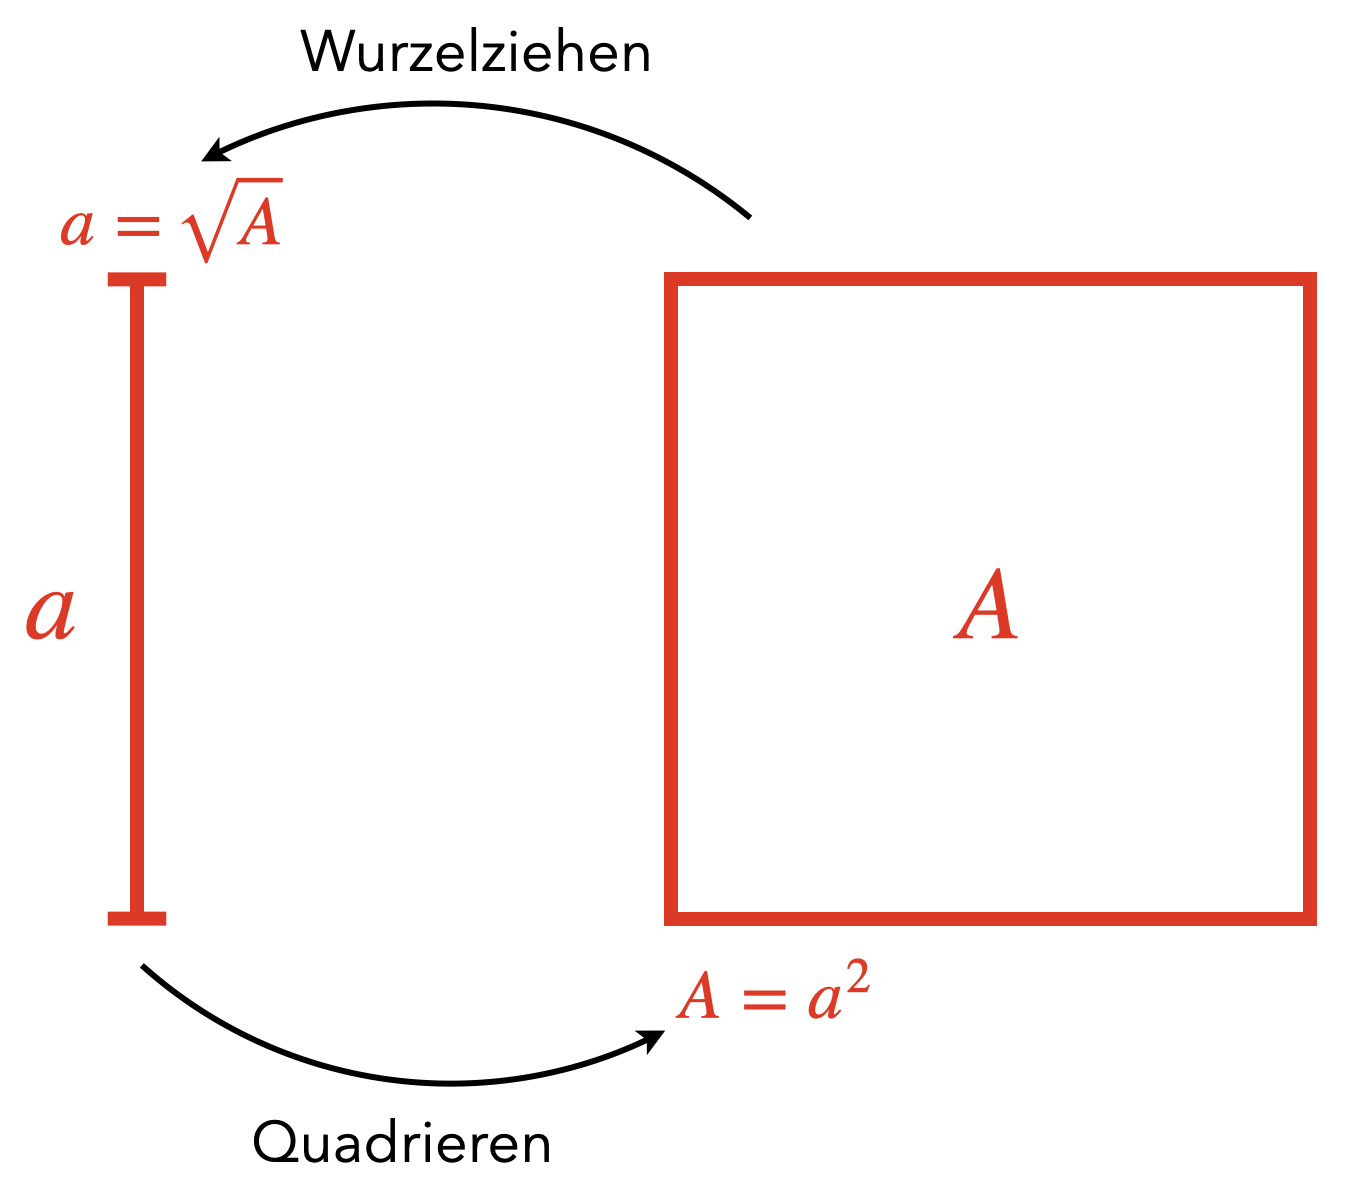
\includegraphics[width=0.5\linewidth]{pictures/9-Wurzel} 

   }

   \caption{(ref:citeLernmodellWurzel)}\label{fig:LernmodellWurzel}
   \end{figure}

  \emph{Achtung! Es ist zwar \((-3)^2 = 9\), aber \(\sqrt{9} \neq -3\), da \(-3\) negativ ist. Außerdem ist \(\sqrt{-9}\) nicht definiert, da \(-9\) negativ ist.}

  Die Auswahl des \textbf{Beispiels} \(\sqrt{9}=3\) war dabei nicht zufällig. Als Einstiegsbeispiel sollte ein leicht nachvollziehbares gewählt werden, daher sollte es sich um (möglichst kleine) natürliche Zahlen handeln und nicht mit Einheiten agiert werden. \(\sqrt{0}\) und \(\sqrt{1}\) fallen weg, da dies Spezialfälle sind, in denen die Werte für Wurzel und Quadrat identisch sind. \(\sqrt{4}\) ist ebenfalls ungünstig, weil dann bei der Erklärung der Umkehrung \(2^2 = 4\) die Ziffer \(2\) doppelt (und in verschiedenen Funktionen) auftaucht, nämlich als Basis und als Exponent. Um derartige \emph{Anfangsverwirrungen} zu vermeiden, ist dann \(\sqrt{9}\) das nächstliegende Einstiegsbeispiel. Entsprechend dem Kontrastprinzip müssen auch nahe \textbf{Gegenbeispiele} wie \(\sqrt{-9}\) sowie \(\sqrt{9}\neq -3\) gebracht werden. Das Variationsprinzip für die Auswahl von Beispielen kann über die verschiedenen Quadrate am Ausgangskonkretum erfüllt werden, in dem dort etwa nicht nur natürliche Zahlen auftreten.
\item
  Anschließend erfolgen vertiefende Übungen und die Betrachtung weiterer Zusammenhänge, anhand derer das Begriffsverständnis vertieft wird.

  \begin{itemize}
  \item
    Beim Wurzelbegriff geht dies insbesondere mit der Zahlbereichserweiterung in die reellen Zahlen einher. Dabei werden Wurzeln als Zahlen (und nicht Seitenlängen) aufgefasst und bspw. auch auf dem Zahlenstrahl geordnet.
  \item
    Eine weitere Anwendung ist die Behandlung der Wurzelgesetze, bspw. \(\sqrt{x\cdot y} = \sqrt{x}\cdot \sqrt{y}\). Bezieht man sich beim Wurzelziehen auf das Umkehren des Quadrierens, so ist eine Begründung mithilfe des Potenzgesetzes \(x^2\cdot y^2 = (x\cdot y)^2\) möglich.
  \end{itemize}
\end{enumerate}

\subsection{Heron-Verfahren}\label{heron-verfahren}

Die Bildungsstandards erfordern die Implementation eines algorithmischen Verfahrens zur Bestimmung von Quadratwurzeln (\citeproc{ref-SekretariatderStandigenKonferenzderKultusministerderLanderinderBundesrepublikDeutschland2022}{Sekretariat der Ständigen Konferenz der Kultusminister der Länder in der Bundesrepublik Deutschland, 2022a, S. 16}), wofür neben der Intervallschachtelung auch das Heron-Verfahren geeignet ist

Die Idee hinter dem Heron-Verfahren besteht darin, dass ein Rechteck mit Flächeninhalt \(A\) immer mehr zu einem Quadrat mit Flächeninhalt \(A\) überführt wird, dessen Seitenlänge zu bestimmen ist.

\begin{itemize}
\tightlist
\item
  In einem ersten Schritt kann eine Seitenlänge \(x_1\) festgelegt und daraus die zweite Seitenlänge \(y_1 = \cfrac{A}{x_1}\) bestimmt werden.\\
\item
  Um die Seitenlängen \emph{anzugleichen} wird in einem nächsten eine neue Seitenlänge \(x_2\) als Durchschnitt der vorherigen Seitenlängen bestimmt: \(x_2 = \cfrac{x_1+y_1}{2}\). So wird sichergestellt, dass das neue Rechteck \emph{quadratischer} als das alte ist. Für die zweite Rechtecksseite gilt entsprechend \(y_2 = \frac{A}{x_2}\).
\item
  Dieses Vorgehen wird nun beliebig weitergeführt, sodass stets gilt: \(x_{n+1} = \cfrac{x_n+y_n}{2} = \cfrac{x_n+\frac{A}{x_n}}{2} = \cfrac{1}{2}\left(x_n + \cfrac{A}{x_n}\right)\)
\end{itemize}

\begin{figure}

{\centering 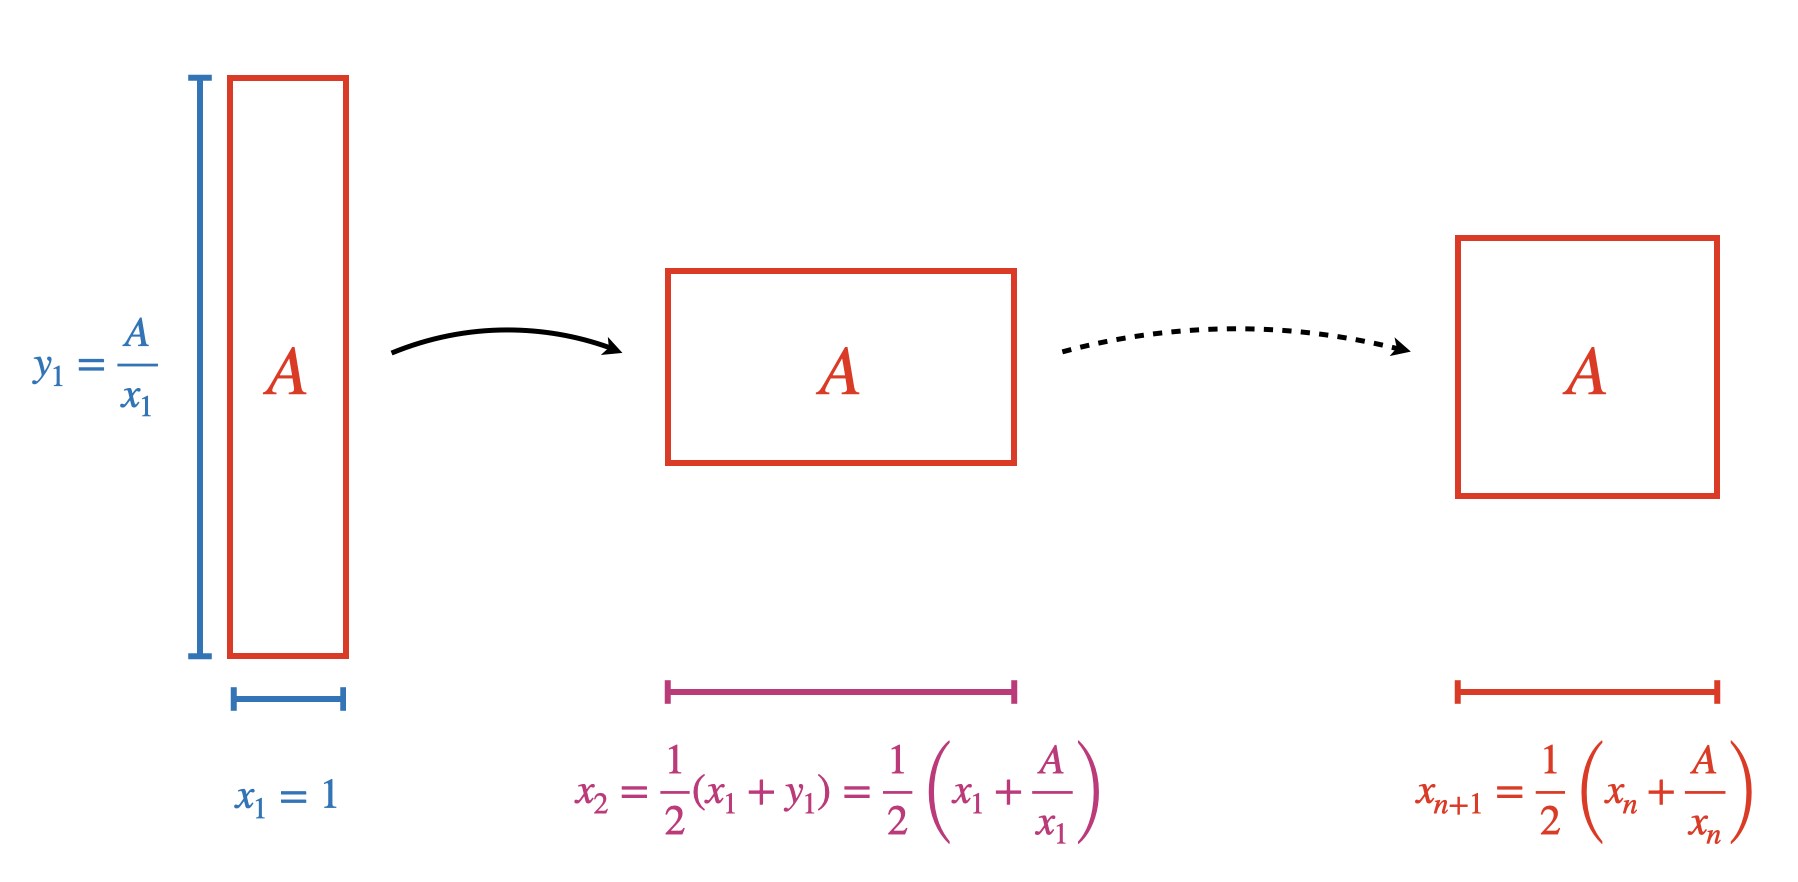
\includegraphics[width=0.9\linewidth]{pictures/9-Heron} 

}

\caption{Visualisierung des Heron-Verfahrens}\label{fig:Heron}
\end{figure}

Mit einem Startwert von bspw. \(x_1 = 1\) ergibt sich als rekursive Bildungsvorschrift für das Heron-Verfahren:

\[x_1 = 1; \quad x_n = \cfrac{1}{2}\left(x_n + \cfrac{A}{x_n}\right)\]

Einen Beweis der Konvergenz dieser Folge sollten Sie aus Ihren Analysis-Veranstaltungen kennen. Eine schrittweise Betrachtung des Folgenverhaltens kann über eine Tabellenkalkulation erfolgen, siehe Abbildung \ref{fig:WurzelTabelle}.

\begin{figure}

{\centering 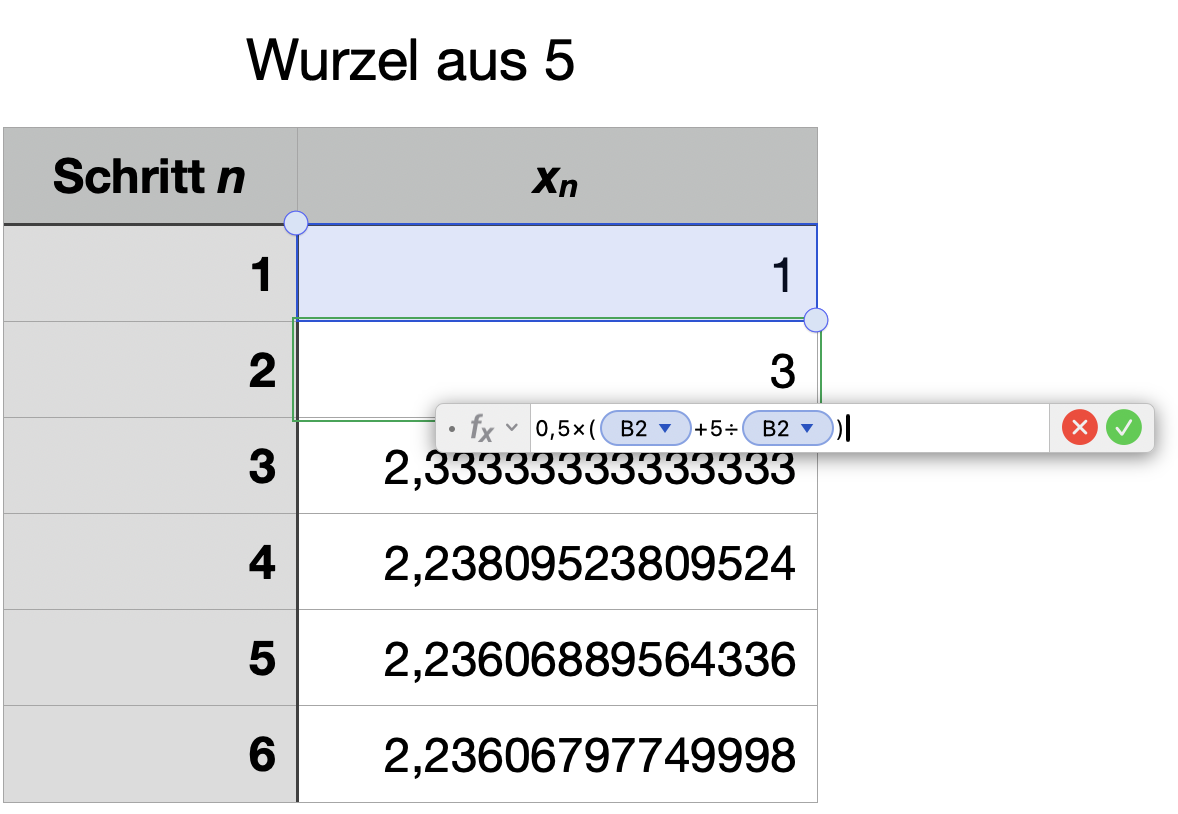
\includegraphics[width=0.5\linewidth]{pictures/9-WurzelTabelle} 

}

\caption{Heron-Verfahren in einer Tabellenkalkulation}\label{fig:WurzelTabelle}
\end{figure}

Eine Implementation in einen Algorithmus bedarf weiterhin einer \emph{Abbruchbedingung}. Dies ist bspw. darüber möglich, dass der Abstand aufeinander folgender Ergebnisse einen bestimmten Wert unterschreiten soll, also \(|x_{n+1}-x_n|<\varepsilon\) für ein vorher festgelegtes \(\varepsilon\) gelten muss. Ein exemplarischer Code für \(\sqrt{5}\) mit einer Genauigkeit von 4 Dezimalstellen sieht folgendermaßen aus:

\begin{Shaded}
\begin{Highlighting}[]
\NormalTok{A }\OtherTok{=} \DecValTok{5}
\NormalTok{x }\OtherTok{=} \DecValTok{1}
\NormalTok{eps }\OtherTok{=} \FloatTok{0.0001}
\ControlFlowTok{while}\NormalTok{(}\FunctionTok{abs}\NormalTok{(x }\SpecialCharTok{{-}}\NormalTok{ (x}\SpecialCharTok{+}\NormalTok{A}\SpecialCharTok{/}\NormalTok{x)}\SpecialCharTok{/}\DecValTok{2}\NormalTok{) }\SpecialCharTok{\textgreater{}}\NormalTok{ eps)\{}
\NormalTok{  x }\OtherTok{=}\NormalTok{ (x}\SpecialCharTok{+}\NormalTok{A}\SpecialCharTok{/}\NormalTok{x)}\SpecialCharTok{/}\DecValTok{2}
\NormalTok{\}}
\end{Highlighting}
\end{Shaded}

\chapter{Analysis}\label{analysis}

\begin{quote}
\textbf{Ziele}

\begin{itemize}
\tightlist
\item
  Sie sind sich bewusst, dass Analysis in Universität und Schule unterschiedlich strukturiert sind und dies in der Schulrealität in einen propädeutischen Grenzwertbegriff mündet.\\
\item
  Sie kennen Grundvorstellungen zum Ableitungsbegriff.\\
\item
  Sie haben einen Einblick in das Unterrichten mit CAS als Werkzeug für die Schülerinnen und Schüler.
\end{itemize}

\textbf{Material}

\begin{itemize}
\tightlist
\item
  Folien zum Kapitel 10 (\href{files/Stoffdidaktik2024-10-Analysis.pdf}{pdf}, \href{files/Stoffdidaktik2024-10-Analysis.key}{Keynote})
\end{itemize}

\textbf{Literaturempfehlungen}

\begin{itemize}
\tightlist
\item
  Greefrath et al. (\citeproc{ref-Greefrath2016}{2016}): \emph{Didaktik der Analysis. Aspekte und Grundvorstellungen zentraler Begriffe}
\item
  Danckwerts \& Vogel (\citeproc{ref-Danckwerts2010}{2010}): \emph{Analysis verständlich unterrichten}
\item
  Tietze et al. (\citeproc{ref-Tietze:2000a}{2000a}): \emph{Mathematikunterricht in der Sekundarstufe II. Band 1: Fachdidaktische Grundfragen, Didaktik der Analysis}
\end{itemize}
\end{quote}

\section{Analysis in der Sek. II}\label{analysis-in-der-sek.-ii}

Der Analysisunterricht in der Schule unterscheidet sich wesentlich von dem in der Hochschule, womit aus fachlicher wie fachdidaktischer Sicht einige Herausforderungen einhergehen. Neben der grundsätzlichen nicht streng deduktiven Herangehensweise werden i.~d.~R. zentrale Begriffe der Analysis im Schulunterricht kaum oder nur propädeutisch-anschaulich behandelt. Die betrifft zunächst einmal den \textbf{Folgen-, Grenzwert- und Stetigkeitsbegriff} (\citeproc{ref-Danckwerts2010}{Danckwerts \& Vogel, 2010, 17~ff.}; \citeproc{ref-Greefrath2016}{Greefrath et al., 2016, 23~ff.}; \citeproc{ref-Tietze:2000a}{Tietze et al., 2000a, 252~ff.}). Der Ableitungsbegriff bedarf bspw. des Grenzwertes des Differenzenquotienten. Ein solcher Grenzwert einer Funktion \(f\) an einer Stelle \(a\) existiert, wenn für alle Folgen \((x_n)_{n\in\mathbb{N}}\) mit \(x_n\rightarrow a\) auch die Folge der Funktionswerte konvergiert, also \(f(x_n)\rightarrow f(a)\). Für den Konvergenzbegriff einer Folge ist nun zum anderen die \textbf{Vollständigkeit der reellen Zahlen} von enormer Bedeutung, was ebenfalls in der Schule nicht in einer derartigen Strenge behandelt wird (siehe z.~B. \citeproc{ref-Danckwerts2010}{Danckwerts \& Vogel, 2010, 27~ff.}). Mathematisch relevant ist für die Konvergenz einer Folge \((x_n)_{n\in\mathbb{N}}\) gegen \(a\) eben nicht nur, dass die Folgeglieder dem \(a\) beliebig nahe kommen, sondern dass \(a\) im betrachteten Zahlbereich tatsächlich existiert. Ein klassisches Beispiel hierfür ist das Heron-Verfahren zum Wurzelbestimmen (vgl. Abschnitt \ref{heron-verfahren}). So liefert die rekursive Folge\(x_{n+1} = \frac{1}{2}\left(x_n + \frac{5}{x_n}\right)\) mit bspw. \(x_0 = 1\) ausschließlich Folgeglieder aus \(\mathbb{Q}\), die sich auch beliebig nahe kommen (eine sogenannte \emph{Cauchy-Folge}), der Grenzwert selbst ist aber \(\sqrt{5}\), was nicht in \(\mathbb{Q}\), sondern nur in \(\mathbb{R}\) liegt.

Ohne derartige zentrale (im fachmathematischen Sinne sauber ausgeprägte) Begriffe Analysisunterricht zu betreiben, bedarf also einer starken Orientierung an den hinter den Begriffen liegenden Grundvorstellungen, damit dennoch ein inhaltlich-anschauliches Verständnis aufgebaut werden kann und der Unterricht nicht zu einem kalkülhaften Vorgehen verkommt. Spezifische Anregungen für einzelne Lerngegenstände bieten die bereits zitierten Quellen.

\section{Grenzwertbegriff}\label{grenzwertbegriff}

\subsection{Fachliche Hinweise}\label{fachliche-hinweise}

Da in der Schule i.~d.~R. keine systematische Behandlung von Folgen erfolgt, ist auch eine formale Definition des Grenzwertbegriffes nicht möglich. Man bedient sich daher -- und so wird es auch im Brandenburgischen Rahmenlehrplan verlangt -- eines \textbf{propädeutischen Zugangs zum Grenzwertbegriff} (vgl. \citeproc{ref-MinisteriumfurBildungJugendundSportdesLandesBrandenburg2022}{Ministerium für Bildung, Jugend und Sport des Landes Brandenburg, 2022b, 25, 28}). Damit ist gemeint, dass der Begriff \emph{vorgebildet} wird, ohne auf eine formale Definition zurückzugreifen. Diese Propädeutik kann dann entweder dazu dienen, später formalisiert zu werden (was beim Grenzwertbegriff jedoch in der Schule normalerweise nicht geschieht, sondern dann erst in einem Mathematikstudium erfolgt) oder aufbauend auf die Propädeutik andere Begrifflichkeiten einzuführen (wie den Ableitungsbegriff). Dabei werden zwar fachliche Lücken hingenommen, aber dennoch versucht, ein Begriffsverständnis aufzubauen.

Formal kann der Grenzwert bzw. die Konvergenz einer Folge definiert werden:

\emph{Eine Folge \(a_n\) heißt konvergent gegen den Grenzwert \(a\), wenn für jedes \(\varepsilon > 0\) ein \(n_0\) existiert, so dass für alle \(n>n_0\) gilt: \(|a_n-a| < \varepsilon\).}

Dabei muss noch festgelegt werden, aus welchem (gemeinsamen) Zahlbereich \(a\) und die \(a_n\) stammen. Die in Abbildung \ref{fig:Grenzwert} dargestellte Visualisierung zum Grenzwertbegriff steht auch als virtuelles Arbeitsmittel über \url{https://www.geogebra.org/m/fwzbx3xa} zur Verfügung.



\begin{figure}

{\centering 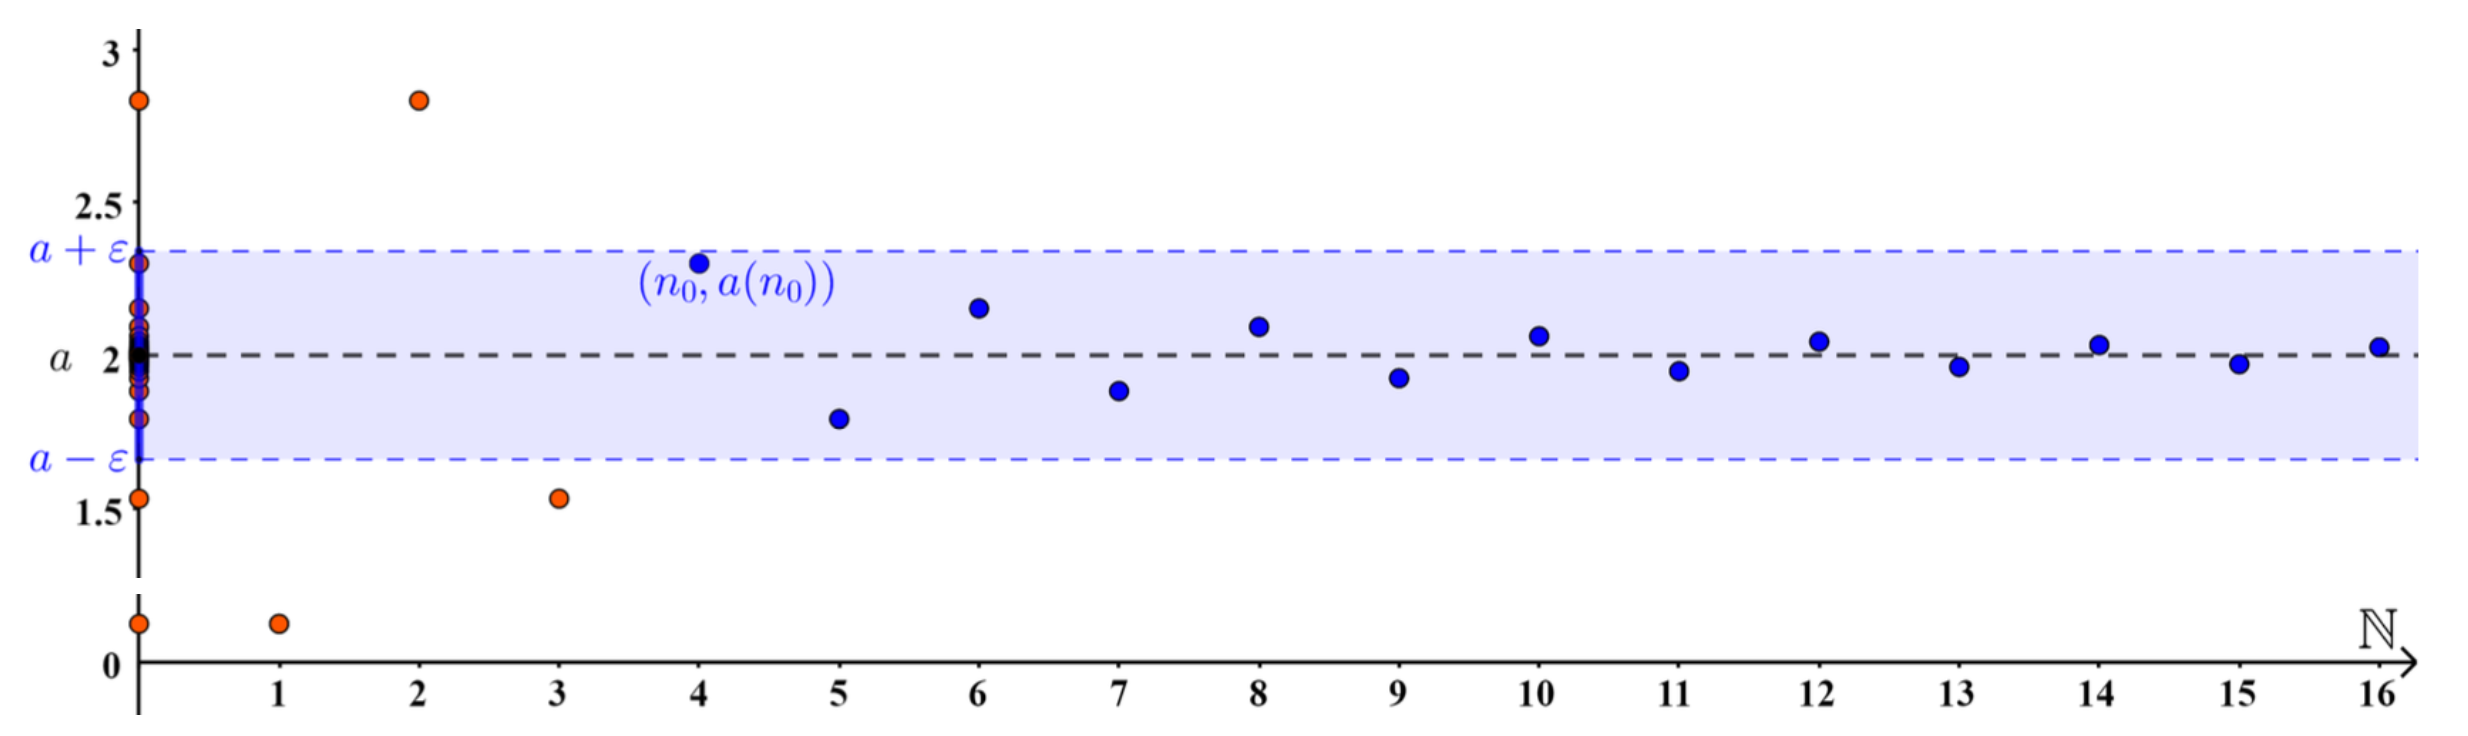
\includegraphics[width=0.9\linewidth]{pictures/12-Grenzwert} 

}

\caption{Visualisierung zum Grenzwertbegriff (\citeproc{ref-Enders2024}{Enders, 2024, S. 36})}\label{fig:Grenzwert}
\end{figure}

Aus der formalen Definition ergeben sich einige Schlussfolgerungen, die -- bei fehlender formaler Definition und einem rein intuitiven Zugang -- häufig mit fehlerhaften Vorstellungen zur Konvergenz und zum Grenzwert einhergehen. Formuliert werden im Folgenden die \emph{mathematisch korrekten} Aussagen.

\begin{itemize}
\item
  Es ist notwendig, dass der \textbf{Grenzwert} \(a\) tatsächlich \textbf{im betrachteten Zahlbereich} auch \textbf{existiert} -- ansonsten kann nicht von Konvergenz gesprochen werden. Es reicht also nicht aus, dass die Folgeglieder einander immer näher kommen.\footnote{Hierfür existiert der Begriff der \emph{Cauchy-Folge}.} Ein typisches Gegenbeispiel hierfür ist die rekursive Folge \(a_{n+1} = \frac{1}{2}\left(a_n+\frac{5}{a_n}\right)\), \(a_0 = 1\), die das Heron-Verfahren beschreibt (siehe Abschnitt \ref{heron-verfahren}). Betrachtet man diese Folge in \(\mathbb{Q}\) (wobei wegen der Grundrechenarten alle Folgeglieder in \(\mathbb{Q}\) bleiben), so ist diese dort nicht konvergent, weil es in \(\mathbb{Q}\) keine Zahl gibt, der die Folgeglieder beliebig nah kommen. Erst in \(\mathbb{R}\) ist diese Folge konvergent gegen den Grenzwert \(\sqrt{5}\).\footnote{Daher kann die Konvergenz von Cauchy-Folgen auch als Charakteristikum von \(\mathbb{R}\) genutzt werden.}
\item
  Die \textbf{Reihenfolge} der Folgeglieder ist \textbf{irrelevant} für die Konvergenz. Da bei einer konvergenten Folge \emph{fast alle} Folgeglieder (also alle bis auf endlich viele) in der \(\varepsilon\)-Umgebung des Grenzwertes liegen, kann bei einer umsortierten Folge das letzte Folgeglied gesucht werden, welches geradeso nicht mehr in der \(\varepsilon\)-Umgebung liegt und anschließend ab dessen Nachfolger das Konvergenzkriterium erfüllt werden.
\item
  Die Folgeglieder können zwar, aber \textbf{müssen dem Grenzwert nicht bei jedem Schritt immer näher kommen}. Bei der Folge \[0,33\quad 0,3\quad 0,3333 \quad 0,333 \quad0,333333 \quad  \ldots\]
  kommt bspw. nur jedes zweite Folgeglied dem Grenzwert \(\frac{1}{3}\) näher, dennoch konvergiert die Folge, weil bei vorgegebener Genauigkeit (\(\varepsilon\)) ein Folgeglied gefunden werden kann (\(a_{n_0}\)), ab dem alle diese Genauigkeit erfüllen (vgl. \citeproc{ref-Ableitinger2013b}{Ableitinger \& Heitzer, 2013, S. 7}).
\item
  Es ist \textbf{irrelevant, ob der Grenzwert erreicht wird oder nicht}. Bei den meisten Beispielen kommen die Folgeglieder dem Grenzwert immer näher, ohne ihn jemals zu erreichen. Dies ist jedoch für die Konvergenz nicht relevant. Es ist durchaus möglich, dass der Grenzwert ab einem bestimmten \(n_0\) tatsächlich erreicht wird (oder auch zwischendurch immer mal wieder). Insofern sind auch konstante Folgen konvergente Folgen.
\end{itemize}

\subsection{Unterrichtliche Zugänge}\label{unterrichtliche-zuguxe4nge}

Um trotz eines \emph{nur} propädeutischen Zugangs zum Grenzwertbegriff Schul-Analysis betreiben zu können, bedarf es (auch schon in der Sekundarstufe I) vielfältiger Erfahrungen zu Grenzprozessen, bei denen die hinter dem Grenzwertbegriff stehenden Ideen sichtbar werden. Greefrath et al. (\citeproc{ref-Greefrath2016}{2016, 107~ff.}) und Ableitinger \& Heitzer (\citeproc{ref-Ableitinger2013b}{2013, S. 3}) führen hierzu vielfältige Vorschläge auf, aus denen hier einige vorgestellt werden sollen.

\begin{itemize}
\tightlist
\item
  In \textbf{geometrischen Situationen} können Grenzprozesse betrachtet werden, etwas bei der näherungsweisen Bestimmung des Flächeninhalts eines Kreises über das Ein- und Umschreiben mittels regelmäßiger \(n\)-Ecke.
\end{itemize}

\begin{figure}

{\centering 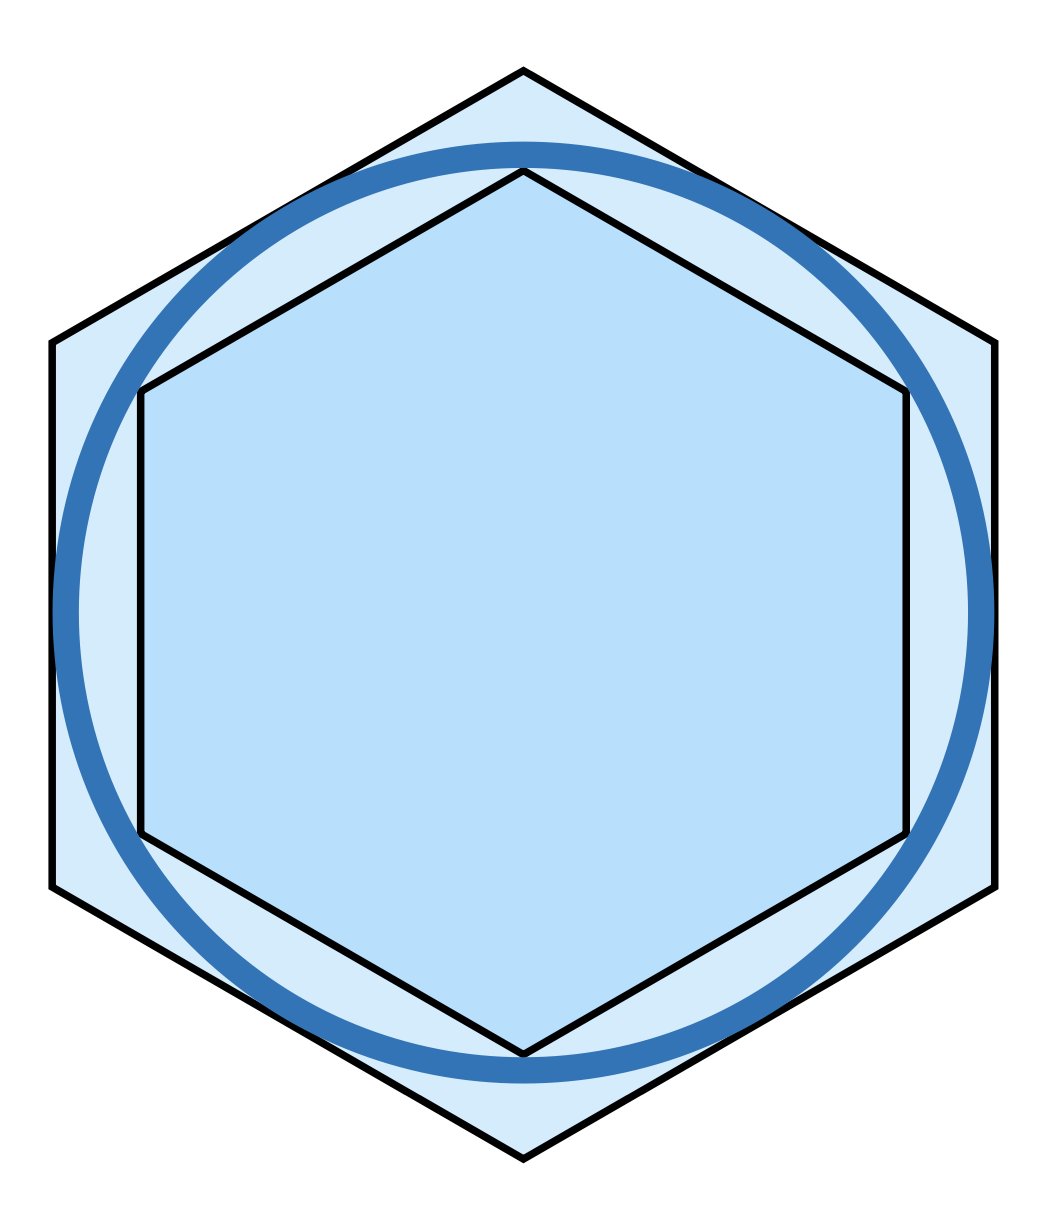
\includegraphics[width=0.5\linewidth]{pictures/12-Kreis} 

}

\caption{Näherungsweise Bestimmung des Kreisflächeninhalts}\label{fig:Kreis}
\end{figure}

\begin{itemize}
\item
  In \textbf{numerischen Situationen} kann die Idee des Grenzprozesses verdeutlicht werden, etwa wenn die Zahl \(\frac{1}{3}\) notiert wird als \(\frac{1}{3} = 0,\bar{3} = 0,3 + 0,03 + 0,003 + \ldots\) oder die Gleichheit von \(0,\bar{9} = 1\) diskutiert wird. Auch die Durchführung einer Intervallschachtelung (siehe Abschnitt \ref{wurzelbehandlung}) fördert das Verständnis für Grenzprozesse. Auch zu Beginn der Sekundarstufe können Erfahrungen gesammelt werden, z.~B. über eine Partneraufgabe, bei der eine Person eine (positive) Zahl nennen muss und die zweite Personen einen Stammbruch (also einen Bruch der Form \(\frac{1}{n}\)) finden muss, der kleiner als die genannte Zahl ist.
\item
  In der \textbf{Kombination geometrischer und numerischer Situationen} liegt ebenfalls Potenzial für die Erfahrung von Grenzprozessen. Die geometrische Interpretation des Heron-Verfahrens (vgl. Abbildung \ref{fig:Heron}) wäre ein Beispiel hierfür. Auch kann die Summation \(2 = 1 + \frac{1}{2} + \frac{1}{4} + \frac{1}{8}+\ldots\) erfahren werden, in dem ein Papierstreifen der Länge \(2\) fortlaufend halbiert wird.
\end{itemize}

\section{Ableitungsbegriff}\label{ableitungsbegriff}

Für den Ableitungsbegriff (einer Funktion an einer Stelle) haben sich sowohl historisch als auch in der fachdidaktischen Literatur zwei wesentliche Vorstellungen herausgebildet (\citeproc{ref-Danckwerts2010}{Danckwerts \& Vogel, 2010, 45~ff.}; \citeproc{ref-Greefrath2016}{Greefrath et al., 2016, 147~ff.})\footnote{Greefrath et al. (\citeproc{ref-Greefrath2016}{2016, 147~ff.}) trennen die lokale Änderungsrate noch von der Vorstellung des Anstiegs der Tangente und beschreiben als vierte Grundvorstellung die Ableitung als Verstärkungsfaktor kleiner Änderungen.}:

\begin{itemize}
\item
  Ableitung als \textbf{lokale Änderungsrate}: Die Ableitung einer Funktion an einer Stelle beschreibt, wie stark sich die Funktionswerte in der Umgebung dieser Stelle verändern. Wird sich dieser Änderungsrate graphisch genähert, erfolgt dies i.~d.~R. durch den Übergang des Anstiegs einer Sekante zu dem einer Tangente\footnote{Zur Diskussion der Vorstellung, was eine Tangente ist, siehe auch Greefrath et al. (\citeproc{ref-Greefrath2016}{2016, S. 149})}, womit die Ableitung über den \textbf{Grenzwert des Differenzenquotienten} \(\lim\limits_{h\rightarrow 0}\cfrac{f(x_0+h)-f(x_0)}{h}\) quantifiziert werden kann und dem \textbf{Anstieg der Tangente} entspricht.

  Diese Sichtweise ermöglicht, den Ableitungbegriff konstruktiv über den Sekanten-Tangenten-Übergang einzuführen und unmittelbar numerisch zu beschreiben. Auch bedienen sich vielfältige Anwendungen (z.~B. Momentan- vs.~Durchschnittsgeschwindigkeit) dieser Vorstellung.
\item
  Ableitung als \textbf{lokale lineare Approximation}: Diese Vorstellung betont noch stärker die Differenzierbarkeit als Eigenschaft einer Funktion, nämlich die Möglichkeit, sie lokal durch eine lineare Funktion annähern zu können. Eine typische Repräsentation ist das Heranzoomen an den Funktionsgraphen, sodass dabei die lokale Linearität besonders deutlich wird. Mathematisch greifbar wird diese Vorstellung darüber, dass sich die Funktion über \(f(x) = f(x_0) + m\cdot x+ r(h)\) beschreiben lässt, wobei der \emph{Fehler} \(r(h)\) so schnell gegen \(0\) geht, dass sogar \(\lim\limits_{h\rightarrow 0}\cfrac{r(h)}{h}=0\) gilt. \(m\) selbst ist dann die Ableitung und der Anstieg der \emph{besten linearen Näherung} -- was natürlich wieder die Tangente an entsprechender Stelle ist.

  Dieses Vorgehen besticht v.~a. durch seine mathematische Verallgemeinerbarkeit für die höherdimensionale Analysis. Auch entspricht es dem Bedürfnis, Prozesse linear zu approximieren (vgl. Abschnitt \ref{beispiel-linearitaet}).
\end{itemize}

\section{Computer-Algebra-Systeme}\label{computer-algebra-systeme}

Insbesondere -- aber nicht ausschließlich -- im Analysis-Unterricht spielt die Verwendung von Computer-Algebra-System (CAS) eine bedeutsame Rolle. In ihrer eigentlich Bezeichnung ist ein CAS ein digitales Werkzeug, das \textbf{symbolische Rechnungen} erlaubt, also bspw. für die Gleichung \(x^2 = 5\) die Lösungen \(\sqrt{5}\) und \(-\sqrt{5}\) ausgeben kann, während ein numerisch rechnendes System hier bspw. \(2,23607\) ausgeben (und die zweite Lösung womöglich sogar unterschlagen) würde.\footnote{Streng genommen ist dieses Beispiel hier im Kapitel falsch, da es eher ein algebraisches Problem ist. Es soll aber dennoch weiter verfolgt werden.}

Insbesondere im schulischen Alltag hat sich »CAS« mittlerweile zum Gattungsbegriff für vielfältige Arten von Taschenrechnern und anderen digitalen Werkzeugen gewandelt. Darunter werden also auch verstanden:

\begin{itemize}
\tightlist
\item
  Wissenschaftliche Taschenrechner (WTR), also Taschenrechner, die wesentliche mathematische Funktionen enthalten (z.~B. auch die Berechnung von Potenzen, dem Sinus usw.) und Punkt- vor Strichrechnung beherrschen.
\item
  Graphikfähige Taschenrechner (GTR), die neben der Funktionalität wissenschaftlicher Taschenrechner auch Funktionsgraphen darstellen können und diese numerisch untersuchen können (z.~B. Schnittpunktbestimmung). Sowohl beim GTR als auch bei CAS handelt es sich in der Regel um programmierbare Taschenrechner, d.~h. es können selbst Algorithmen implementiert werden, die dann als Funktion zur Verfügung stehen.
\item
  Tabellenkalkulationen (TK), in denen mit strukturiert notierten Daten gerechnet werden kann.
\item
  Dynamische Geometriesysteme (DGS), die die Möglichkeit bieten, geometrische Konstruktionen darzustellen. Mehr dazu finden Sie in Abschnitt \ref{dynamische-geometriesysteme}.
\end{itemize}

\subsection{Software und Hardware}\label{software-und-hardware}

Am weitesten sind an Schulen derzeit noch »echte« \textbf{Taschenrechner} mit CAS-Funktionalität verbreitet, i.~d.~R. von den Firmen Casio, TI, HP oder Sharp. Einige Bundesländer formulieren Voraussetzungen, über welche Funktionalitäten derartige Systeme verfügen müssen (und nicht verfügen dürfen), so dass sie auch in Prüfungssituationen verwendet werden können. Ab dem Prüfungsjahr 2030 soll es bundesweit einheitliche Voraussetzungen für sogenannte \textbf{modulare Mathematiksysteme (MMS)} geben, siehe \url{https://www.iqb.hu-berlin.de/abitur/dokumente/mathematik/}.

Stärkere Verbreitung finden mittlerweile \textbf{Software-Lösungen}, die spezifisch für \textbf{schulische Zwecke} entwickelt worden sind, z.~B. die CAS-Funktion von GeoGebra\footnote{\url{https://www.geogebra.org/cas}}. Auch Apps wie Photomath\footnote{\url{https://photomath.com}} können als CAS aufgefasst werden. In Schulen i.~d.~R. nicht verbreitet sind \textbf{professionelle kommerzielle Angebote} wie Maple oder Matheamtica. Es gibt jedoch auch \textbf{freie CAS-Software}, die zwar nicht explizit für schulische Zwecke entwickelt worden ist, aber dennoch für Schülerinnen und Schüler zugänglich ist und (aus fachmathematischer Sicht) »echte« CAS-Lösungen darstellt. Hierzu gehören etwa Yacas\footnote{\url{http://www.yacas.org}} oder Sage\footnote{\url{https://sagecell.sagemath.org}}, die wie GeoGebra über Online-Editoren verfügen.

\subsection{Bedienung schulen}\label{bedienung-schulen}

Das Lernen der \textbf{Bedienung} eines CAS erfolgt nicht »nebenbei« zum Lernen der mathematischen Zusammenhänge, sondern muss \textbf{explizter Lerngegenstand} werden. Hierzu ist es notwendig, die entsprechenden CAS-Befehle mit den dahinter liegenden mathematischen Handlungsfolgen in Bezug zu bringen, bspw. über eine Versprachlichung des Befehls und seiner Bestandteile.

\begin{figure}

{\centering 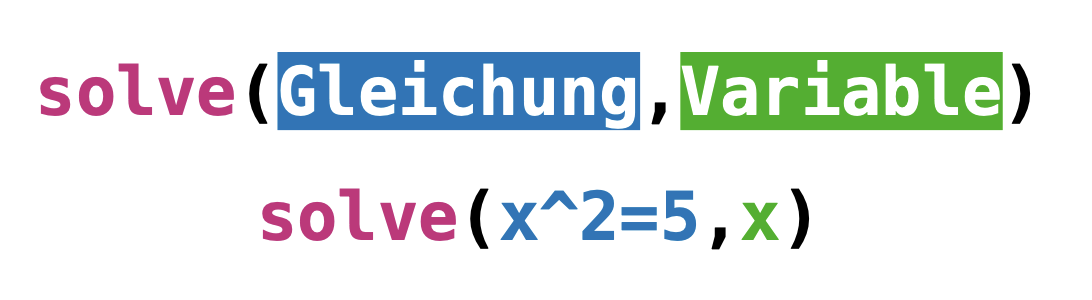
\includegraphics[width=0.5\linewidth]{pictures/12-Befehl} 

}

\caption{CAS-Befehl zum Lösen einer Gleichung}\label{fig:Befehl}
\end{figure}

Für den in Abbildung \ref{fig:Befehl} dargestellten Befehl kann als Erläuterung dienen: »Der Befehl {löst} die Gleichung {\(x^2 = 5\)}, d.~h. es werden diejenigen Werte {für \(x\)} gesucht, für die die Gleichung eine wahre Aussage ergibt.«

Derartige Bedienschulungen können dann wieder durch Identifizierungs- und Realisierungs- sowie Festigungsaufgaben angeeignet werden, das heißt u.~a.:

\begin{itemize}
\tightlist
\item
  Zu vorgegebenen Beschreibungen müssen entsprechende Befehle ins CAS eingegeben werden.
\item
  Zu gegebenen Befehle soll beschrieben werden, wofür diese dienlich sind.
\item
  Befehle oder die in ihnen enthaltenen Bestandteile müssen variiert werden und die Einflüsse der Variation untersucht bzw. beschrieben werden.
\end{itemize}

Weiterhin ist es notwendig, die \textbf{hinter dem Befehl liegende Mathematik} nachvollziehen zu können. Es reicht also nicht aus, das CAS als \textbf{Black-Box} aufzufassen, dass aus der Eingabe \texttt{solve(x\^{}2=5,x)} \emph{irgendwie} die Ausgabe \texttt{√5,-√5} erzeugt, sondern es sollten stets die dahinterliegenden Prozesse hinterfragt werden. Dies kann auch über die Darstellung von (Pseudo-)Algorithmen erfolgen, wobei nicht jeder Schritt (oder nicht einmal der komplette Algorithmus) der tatsächlichen algorithmische Umsetzung im Hintergrund des CAS entsprechen muss, solange er mathematisch nachvollziehbar ist. Im genannten Beispiel könnte ein solcher Pseudoalgorithmus, der nach der Eingabe des Befehls \texttt{solve(x\^{}2=5,x)} abläuft, lauten:

\begin{enumerate}
\def\labelenumi{\arabic{enumi}.}
\tightlist
\item
  Prüfe, ob es sich um eine quadratische Gleichung handelt.
\item
  Bringe die Gleichung in die Form \(0 = x^2+px+q\).
\item
  Bestimmte \(p\) und \(q\).
\item
  Gibt die Lösungen \(-\frac{p}{2}+\sqrt{\left(\frac{p}{2}\right)^2-q}\) und \(-\frac{p}{2}-\sqrt{\left(\frac{p}{2}\right)^2-q}\) aus.
\end{enumerate}

\subsection{Neue Aufgabenkultur}\label{neue-aufgabenkultur}

In der Verwendung von CAS ergibt sich die Notwendigkeit einer neuen Aufgabenkultur, da eine klassische Aufgabe der Art »Ermittle die Lösungsmenge der Gleichung \(x^2 = 5\)« mithilfe eines CAS, sofern der entsprechende Befehl bekannt ist, keine mathematisch-gedankliche Herausforderung mehr darstellt.

\begin{itemize}
\item
  Kortenkamp (\citeproc{ref-Kortenkamp2007}{2007}) schlägt beispielsweise vor, das \textbf{CAS als Überprüfungsinstrument} zu verwenden, um selbst erzeugte Aufgaben zu prüfen. Im oben genannten Beispiel könnte eine Aufgabenstellung lauten: »Stell eine quadratische Gleichung auf, die \(\sqrt{5}\) als Lösung hat.« Solche Aufgaben können dann schrittweise variiert und komplexer gestaltet werden (»Stell eine quadratische Gleichung auf, die nur \(\sqrt{5}\) als Lösung hat« usw.).
\item
  Die von einem CAS ausgegebene \textbf{Lösung} kann wiederum \textbf{als Anlass} genutzt werden, mathematische Fragen zu stellen. Im obigen Beispiel wäre möglich zu fragen: »Warum gibt das CAS zwei Lösungen aus?«, »Wie hängen die Lösungen miteinander zusammen?« o.~ä. Derartige Fragen sollten auf die hinter der Aufgabe liegende Struktur hinzielen.
\item
  Nicht zu verschweigen ist auch, dass sich durch die Verwendung von CAS (und anderen Taschenrechnern) sogenannte \textbf{»oHiMi«-Aufgaben} etabliert haben, also Aufgaben, die \textbf{o}hne \textbf{Hi}lfs\textbf{mi}ttel zu bearbeiten sind. Dahinter steckt die Auffassung, dass Schülerinnen und Schüler über gewisse Basiskenntnisse und -fertigkeiten verfügen sollten, die dann auch in Prüfungssituationen abgefragt werden. Entsprechende Erwartungen sind in den Lehrplänen formuliert, in Brandenburg z.~B. über eine Anlage zum Rahmenlehrplan der gymnasialen Oberstufe (\citeproc{ref-MinisteriumfurBildungJugendundSportdesLandesBrandenburg2022a}{Ministerium für Bildung, Jugend und Sport des Landes Brandenburg, 2022a}).
\end{itemize}

Eine etwas ausführlichere -- und auch über 15 Jahre nach ihrer Entstehung immer noch nicht vollumfänglich im Schulalltag angekommene -- Diskussion zum Einfluss von CAS und Graphikfähigen Taschenrechnern auf die Aufgabenkultur findet sich bei Heinrich (\citeproc{ref-Heinrich2007}{2007}).

\appendix


\chapter{Sammlung von Lernbereichen}\label{sammlung-von-lernbereichen}

Die folgende Sammlung von Lernbereichen ist im Rahmen des Seminars zur Stoffdidaktik-Veranstaltung entstanden und berücksichtigt die Brandenburger Rahmenlehrpläne für die Klassenstufen 1~--~10 bzw. die gymnasiale Oberstufe (\citeproc{ref-MinisteriumfurBildungJugendundSportdesLandesBrandenburg2022}{Ministerium für Bildung, Jugend und Sport des Landes Brandenburg, 2022b}, \citeproc{ref-MinisteriumfuerBildungJugendundSportdesLandesBrandenburg2023}{2023}).

Die Darstellung nach Klassenstufen orientiert sich an den Niveaustufen für den gymnasialen Bildungsgang (vgl. \citeproc{ref-MinisteriumfuerBildungJugendundSportdesLandesBrandenburg2023}{Ministerium für Bildung, Jugend und Sport des Landes Brandenburg, 2023, S. 20}).

Die Übersicht kann als \href{files/Stoffdidaktik2024-SammlungLernbereiche.pdf}{pdf-Datei} heruntergeladen werden.

\chapter{Beispiel: Arithmetisches Mittel}\label{beispiel-arithmetisches-mittel}

\begin{quote}
\textbf{Ziele}

\begin{itemize}
\tightlist
\item
  Sie können die Strukturierung einer Unterrichtsstunde zum arithmetischen Mittel nachvollziehen.\\
\item
  Sie erkennen den Nutzen stoffdidaktischer Analysen und tätigkeitstheoretischer Modelle für die strukturierte Planung von Mathematikunterricht.\\
\item
  Sie haben einen Einblick in die Gestaltung von Arbeitsmitteln am
  Beispiel des arithmetischen Mittels.
\end{itemize}

\textbf{Material}

\begin{itemize}
\tightlist
\item
  Folien zum Anhang (\href{files/Stoffdidaktik2024-B-ArithmetischesMittel.pdf}{pdf}, \href{files/Stoffdidaktik2024-B-ArithmetischesMittel.key}{Keynote})
\item
  Virtuelles Arbeitsmittel zum Medien und arithmetischen Mittel (\href{files/Stoffdidaktik2024-B-Lagemasse.html}{html}, \href{files/Stoffdidaktik2024-B-Lagemasse.cdy}{Cinderella})
\end{itemize}
\end{quote}

In diesem Kapitel sollen die in den Kapiteln zur Sotffdidaktischen Analyse und zur Gestaltung von Lernprozessen dargestellten Theorien auf die Planung einer 45-minütigen Unterrichtsstunde zum arithmetischen Mittel angewandt werden. Es handelt sich dabei nicht um eine ausführliche Unterrichtsplanung -- für diese wäre mindestens noch eine Bedingungsanalyse der zu unterrichtenden Klasse und eine ausführlichere didaktisch-methodische Diskussion notwendig. Vielmehr soll \emph{im Groben} dargestellt werden, welche theoriebasierten Gedankengänge in die Strukturierung einer Unterrichtsstunde fließen können.

\section{Stoffdidaktische Hintergründe}\label{stoffdidaktische-hintergruxfcnde}

Das \textcolor{formalColor}{arithmetische Mittel} ist ein Lagemaß und ist daher in den Lernbereich der \textbf{Lage- und Streumaße} einzuordnen. Bedeutsame Begriffe sind demnach das \emph{arithmetische Mittel}, der \emph{Median} und der \emph{Modalwert}, die \emph{Spannweite}, \emph{Varianz} und \emph{Standardabweichung}, sowie ggf. noch das \emph{untere} und \emph{obere Quartil} bzw. \emph{Ausreißer}. Sachverhalte und Verfahren spielen in dem Lernbereich keine so große Rolle. Gegebenenfalls ist mit Blick auf die Oberstufe und die Anwendung im Zusammenhang mit Erwartungswerten noch der \emph{Steinersche Verschiebungssatz}\footnote{\(\sum\limits_{i=1}^n (x_i-\bar{x})^2 = \left(\sum\limits_{i=1}^nx_i^2\right)-n\bar{x}^2\)} von Relevanz.

Als Lagemaß bedarf das arithmetische Mittel \textbf{metrisch skalierter Daten}, also Daten, mit denen aufgrund ihrer inneren Anordnung und Skalierung gerechnet werden darf.\footnote{Das ist auch der Grund, weshalb das arithmetische Mittel streng genommen nicht geeignet ist einen Notendurchschnitt zu bestimmen, da die Abstände zwischen den Notenstufen nicht gleich sind.} Dem gegenüber stehen \textbf{ordinal skalierte Daten}, die sich \emph{nur} in eine Reihenfolge bringen lassen oder \textbf{nominal skalierte Daten}, die mithilfe von Bezeichnungen beschrieben werden. Dabei kann jede metrische Skala auch als ordinale und jede ordinale Skala auch als nominale Skala aufgefasst werden. Diese Unterscheidung ist insbesondere dann relevant, wenn die verschiedenen Lagemaße miteinander verglichen werden, da für ordinal skalierte Daten auch der Median und für nominal skalierte Daten der Modalwert bestimmt werden können.

\begin{figure}

{\centering 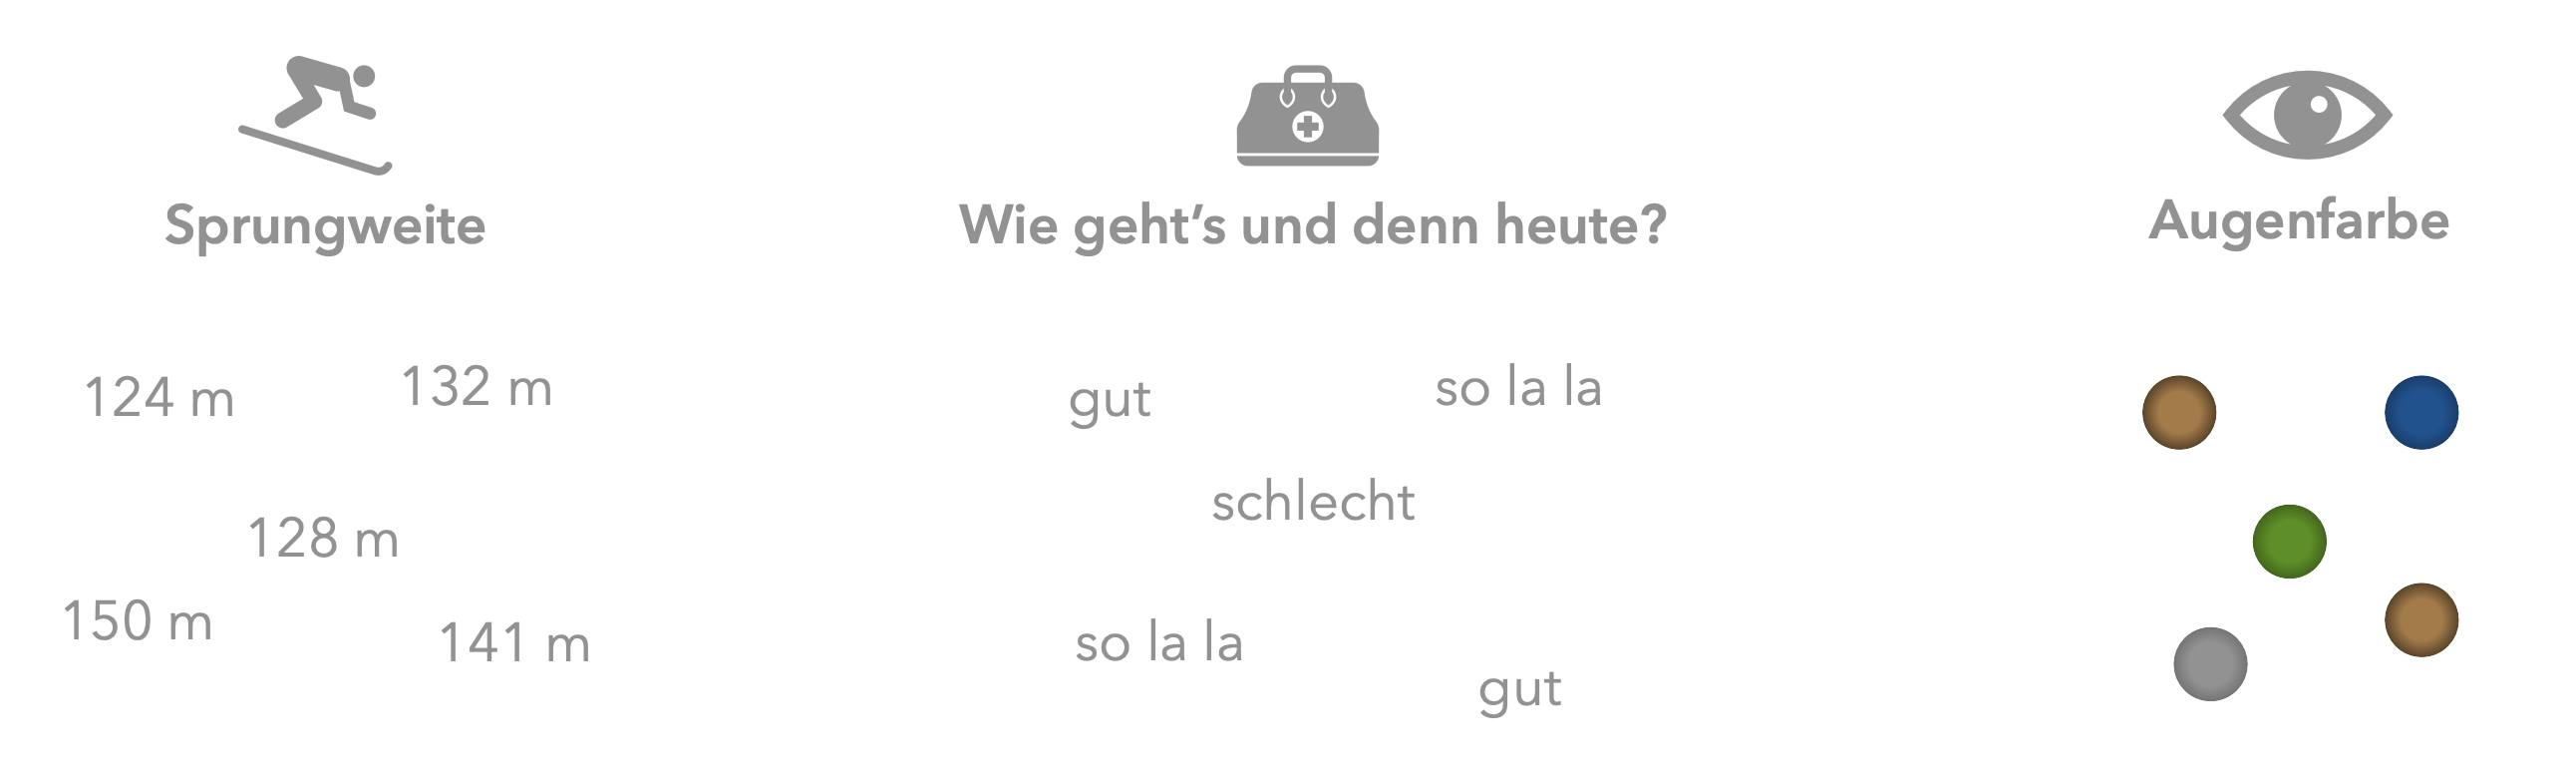
\includegraphics[width=0.9\linewidth]{pictures/B-Skalen} 

}

\caption{Beispiele für metrische, ordinale und nominale Skalen}\label{fig:Skalen}
\end{figure}

Hat man eine Messreihe mit den \(n\) Daten \(x_1,x_2,\ldots,x_n\) gegeben, lässt sich das arithmetische Mittel \(\bar{x}\) berechnen über

\[\bar{x} = \frac{x_1+x_2+\ldots + x_n}{n} = \frac{\sum\limits_{i=1}^n x_i}{n} = \sum_{i=1}^n \frac{x_i}{n}\]

In der Schule üblich ist die erste Schreibweise, in der keine Summenzeichen verwendet werden. Es gibt auch die Möglichkeit, die Berechnung nur über ihre Vorschrift einzuführen: »Bilde die Summe aller Werte und dividiere durch die Anzahl aller Werte.« (vgl. \citeproc{ref-Kruger2015}{Krüger et al., 2015, S. 56}).

Diese Sichtweise wird in der Oberstufe für nicht-diskrete Daten mithilfe des Integrals erweitert über \(\bar{x} = \frac{\int\limits_a^b f(x)}{b-a}\).

Nach Krüger et al. (\citeproc{ref-Kruger2015}{2015, 56~f.}) enthält das arithmetische Mittel folgende Aspekte:

\begin{itemize}
\tightlist
\item
  Es handelt sich um eine \textbf{fiktive Größe}, die von keinem der Messwerte erreicht werden muss bzw. im Kontext auch gar nicht realistisch erscheinen muss (wenn es sich zum beispiel um Messungen mit natürlischen Zahlen handelt, kann das arithmetische Mittel dennoch eine Bruchzahl sein).
\item
  Das arithmetische Mittel kann als \textbf{Vergleichswert} eines jeden Messwertes aufgefasst werden.
\item
  Damit ist das arithmetische Mittel auch ein \textbf{Prognosewert}, der eine Einschätzung darüber gibt, in welcher Größenordnung ein Messwert (vermutlich) liegen wird.
\item
  Außerdem kann das arithmetische Mittel als \textbf{repräsentativer Wert} einer kompletten Messreihe aufgefasst werden -- also die eigentliche Eigenschaft des Lagemaßes annehmen.
\end{itemize}

Als \textcolor{semanticColor}{Grundvorstellungen} werden von Krüger et al. (\citeproc{ref-Kruger2015}{2015, 57~ff.}) genannt, dass das arithmetische Mittel als \textbf{Ausgleichwert} sowie als \textbf{Wert einer gleichmäßigen Verteilung} aufgefasst werden kann. Letzere Vorstellung ermöglicht die Repräsentation, die \(n\) Werte als Strecken nebeneinander und im Vergleich dazu \(n\) gleich lange Strecken mit gleicher Gesamtlänge darzustellen (siehe Abbldung \ref{fig:Hefter}).

Hinsichtlich der \textcolor{concreteColor}{Kernfragen} bietet es sich an, den Nuten von Lage- und Streumaßen zu hinterfragen:

\begin{itemize}
\tightlist
\item
  Allgemein dienen Lage- und Streumaße -- neben Diagrammen -- dem Vergleich statistischer Erhebungen, also könnte eine Kernfrage lauten: \textbf{Wie kann ich statistische Erhebungen rechnerisch miteinander vergleichen?}
\item
  Konkret auf Lagemaße bezogen, ließe sich die präzisieren: \textbf{Wie kann ich die vielen Ergebnisse einer Messreihe mit nur einem Wert beschreiben?}
\item
  Die Besonderheit des arithmetischen Mittel, dass dieses bei metrisch skalierten Daten tatsöchlich eine berechnet Zahl ergibt, könnte folgendertmaßen betont werden: \textbf{Wie kann ich das durchschnittel Ergbnis einer Messreihe \emph{berechnen}?}
\end{itemize}

Als sinnstifender Kontext bieten sich \textbf{Sportliche Leistungen} an, da diese den Schülerinnen und Schülern vertraut sind (\emph{Lebensweltbezug}), Lage- und Streumaße tatsächlich zu ihrem Vergleich herangezogen werden (\emph{Authentizität}) und über vielfältige Sportarten die weiteren Lage- und Streumaße am Kontext besprochen werden können (\emph{Reichhaltigkeit}). Außerdem bietet sich dieser Kontext für fächerübergreifende oder projektartige Herangehensweisen an.

\section{Kompetenzziele}\label{kompetenzziele}

Im Gegensatz zu den \textbf{Lernzielen}, die ein psychisches Konstrukt der Lernenden sind (vgl. Abschnitt \ref{lernzielbildung}), beschreiben die \textbf{Kompetenzziele}, über welche Kompetenzen die Schülerinnen und Schüler am Ende der Unterrichtsstunde neu verfügen sollen. Beim konkreten Lerngegenstand sind für eine 45-minütige Unterrichtsstudne realistisch:

\begin{itemize}
\tightlist
\item
  Die Schülerinnen und Schüler können das arithmetische Mittel einer Messreihe berechnen.\\
\item
  Die Schülerinnen und Schüler können erklären, wofür man des arithmetischen Mittel benötigt.
\end{itemize}

\section{Unterrichtsphasen}\label{unterrichtsphasen}

Im folgenden wird davon ausgegangen, dass für diese Unterrichtsstunde keine explizite \textbf{Sicherung des Ausgangsniveaus} notwendig ist. Diese Entscheidung kann niemals pauschal, sondern muss immer abhängig von der konkreten Klasse und der Lehr-Lern-Situation getroffen werden. Hier wird von einer Klasse ausgegangen, die das Addieren und Dividieren (was für die Berechnung des arithmetischen Mittels notwendig ist) beherrscht und aufgrund des aktuellen Mathematikunterrichts Erfahrungen im Umgang mit Daten hat.

\subsection{Motivierung und Zielbildung}\label{motivierung-und-zielbildung-1}

Als auszuprägended \textbf{Lernziel} bietet sich einer Orientierung an der Kernfrage an (vgl. Abschnitt \ref{bezuege-zur-stoffdidaktik}), so dass am Ende dieser Unterrichtsphase formuliert werden sollte: \emph{Wir wollen lernen, wie man das durchschnittliche Ergebnis einer Messreihe berechnen kann.}

Im Kontext des Vergleichs sportlicher Leistung kann nun eine \textbf{Anforderungssituation in der Zone der nächsten Entwicklung} gesucht werden. Hierbei sollte nicht offensichtlich sichtbar sein, welche Person die besseren durchschnittlichen Leistungen erbracht hat, um eine Motivation für die Beschäftigung mit dem Lerngegenstand zu schaffen. Das heißt, wenn bspw. die sportlichen Leistungen zweier Personen miteinander verglichen werden:

\begin{itemize}
\tightlist
\item
  Die beiden Personen dürfen nicht gleich viele Versuche durchgeführt haben, da sonst einfach die Summe der Ergebnisse miteinander verglichen werden kann.
\item
  Die Messreihe mit weniger Daten darf keine größere Summe aufweisen als die Messreihe mit mehr Daten, da sonst eine Berechnung zum Vergleich nicht notwendig ist.
\end{itemize}

Eine mögliche \textbf{Aufgabenstellung} könnte lauten:

\emph{Mara und Lasse haben Weitsprung geübt. Wer von den beiden ist besser?}\\
\emph{Maras Sprungweiten: 3,20 m; 1,90 m; 3,00 m; 2,90 m}\\
\emph{Lasses Sprungweiten: 3,10 m; 2,90 m; 2,70 m; 2,60 m; 3,00 m}

Alternativ wäre es auch möglich, mit den Schülerinnen und Schülern Messwerte aufzunehmen. Diese müssen dann jedoch die oben genannten Kriterien erfüllen. Eine Entscheidung, welcher Weg getroffen wird, ist auch von den konkreten Rahmenbedingungen abhängig.

Eine mögliche \textbf{Abfolge} zur Gestaltung dieser Phase könnte sein:

\begin{enumerate}
\def\labelenumi{\arabic{enumi}.}
\tightlist
\item
  Die in der Aufgabenstellung präsentierte Situation wird im Plenung oder im Rahmen einer Murmelphase analysiert und es werden Vorschläge zur Lösung eingeholt. Möglich Impulse könnten sein: \emph{Wie kann ich die beiden miteinander vergleichen?} \emph{Was heißt es, besser zu sein?}
\item
  Anschließend kann das Lernziel gemeinsam im Gespräch herausgearbeitet werden. Ergänzend zur obigen Formulierung bietet es sich an, zu betonen: \emph{Wir wollen nicht nur herausfinden,} \textbf{\emph{wer}} \emph{besser ist, sondern wollen lernen,} \textbf{\emph{wie}} \emph{wir das herausfinden.}
\end{enumerate}

\subsection{Stoffvermittlung}\label{stoffvermittlung}

Da die Vorgehensweise zur Berechnung des arithmetischen Mittels nicht allzu kompliziert ist, bietet es sich an, dass diese von den Schülerinnen und Schülern selbstständig über einen \textbf{geführten Arbeitsauftrag} erarbeitet wird. Um damit die spätere Definition und eine geeignete Repräsentation vorzubereiten, kann diese im Arbeitsauftrag bereits enthalten sein.

\begin{itemize}
\tightlist
\item
  \emph{Begründe, warum es nicht ausreicht, die Gesamtweiten von Mara und Lasse miteinander zu vergleichen.}\\
\item
  \emph{Zeichne dir die Sprungweiten für Mara in einem geeigneten Maßstab nebeneinander. Stell dir vor, Mara wäre jedes mal gleich weit gesprungen. Wie weit wäre das bei der gleichen Gesamtweise jeweils gewesen?}
\end{itemize}

\begin{center}
\includegraphics[width=0.5\linewidth]{pictures/B-Einfuehrung} \end{center}

\begin{itemize}
\tightlist
\item
  \emph{Wiederhole das Vorgehen mit Lasses Sprungweiten vergleiche anschließend die durchschnittlichen Leistungen der beiden.}
\end{itemize}

Die Bearbeitung dieser Aufgabenfolge bietet sich in Parnerarbeit an. Anschließend kann im Plenum die systematische Stofferarbeitung erfolgen:

\begin{enumerate}
\def\labelenumi{\arabic{enumi}.}
\tightlist
\item
  Es wird zunächst kurz die Begründung zum ersten Arbeitsauftrag besprochen.
\item
  Anschließend beschreiben einzelne Schülerinnen und Schüler ihr Vorgehen beim zweiten Arbeitsauftrag. Dies unterstützt auch den Übergang von der materialisierten zur sprachlichen Handlung zur Aneignung des Lerngegenstands (vgl. Abschnitt \ref{ausfuehren-und-verinnerlichen}).
\item
  Die Resultate zum dritten Arbeitsauftrag sollten selbstverständlich auch besprochen werden. An dieser Stelle muss jedoch darauf aufmerksam gemacht werden, dass das konkrete Ergebnis gar nicht so relevant ist wie der \emph{Weg}, auf dem zu den Ergebnis gekommen wurde. Hier bietet sich daher ein Bezug zum ursprünglich ausgearbeiteten Lernziel an.
\item
  Nun kann unabhängig vom Sport-Kontext das allgemeine Vorgehen herausgearbeitet werden, also dass zunächst alle Werte addiert und anschließend durch die Anzahl der Werte dividiert wird. Auch hier können entsprechende Impule genutzt werden: \emph{Was muss man also allgemein tun, wenn man eine Messreihe hat und den durchschnittlichen Wert bestimmen möchte?}
\item
  Erst nach dieser inhaltlichen Erarbeitung sollte der \emph{Bezeichner} »arithmetisches Mittel« eingeführt werden, da der neue Begriff nun mit einem inhaltlichen Verständnis verknüpft werden kann.
\item
  Anschließend kann eine Defition und Vorgehensweise zur Berechnung des arithmetischen Mittels notiert werden. Hier bietet es sich an, wieder auf die bereits verwendete Repräsentation einzugehen. Abbildung \ref{fig:Hefter} zeigt einen möglichen Hefteraufschrieb.
\end{enumerate}

\begin{figure}

{\centering 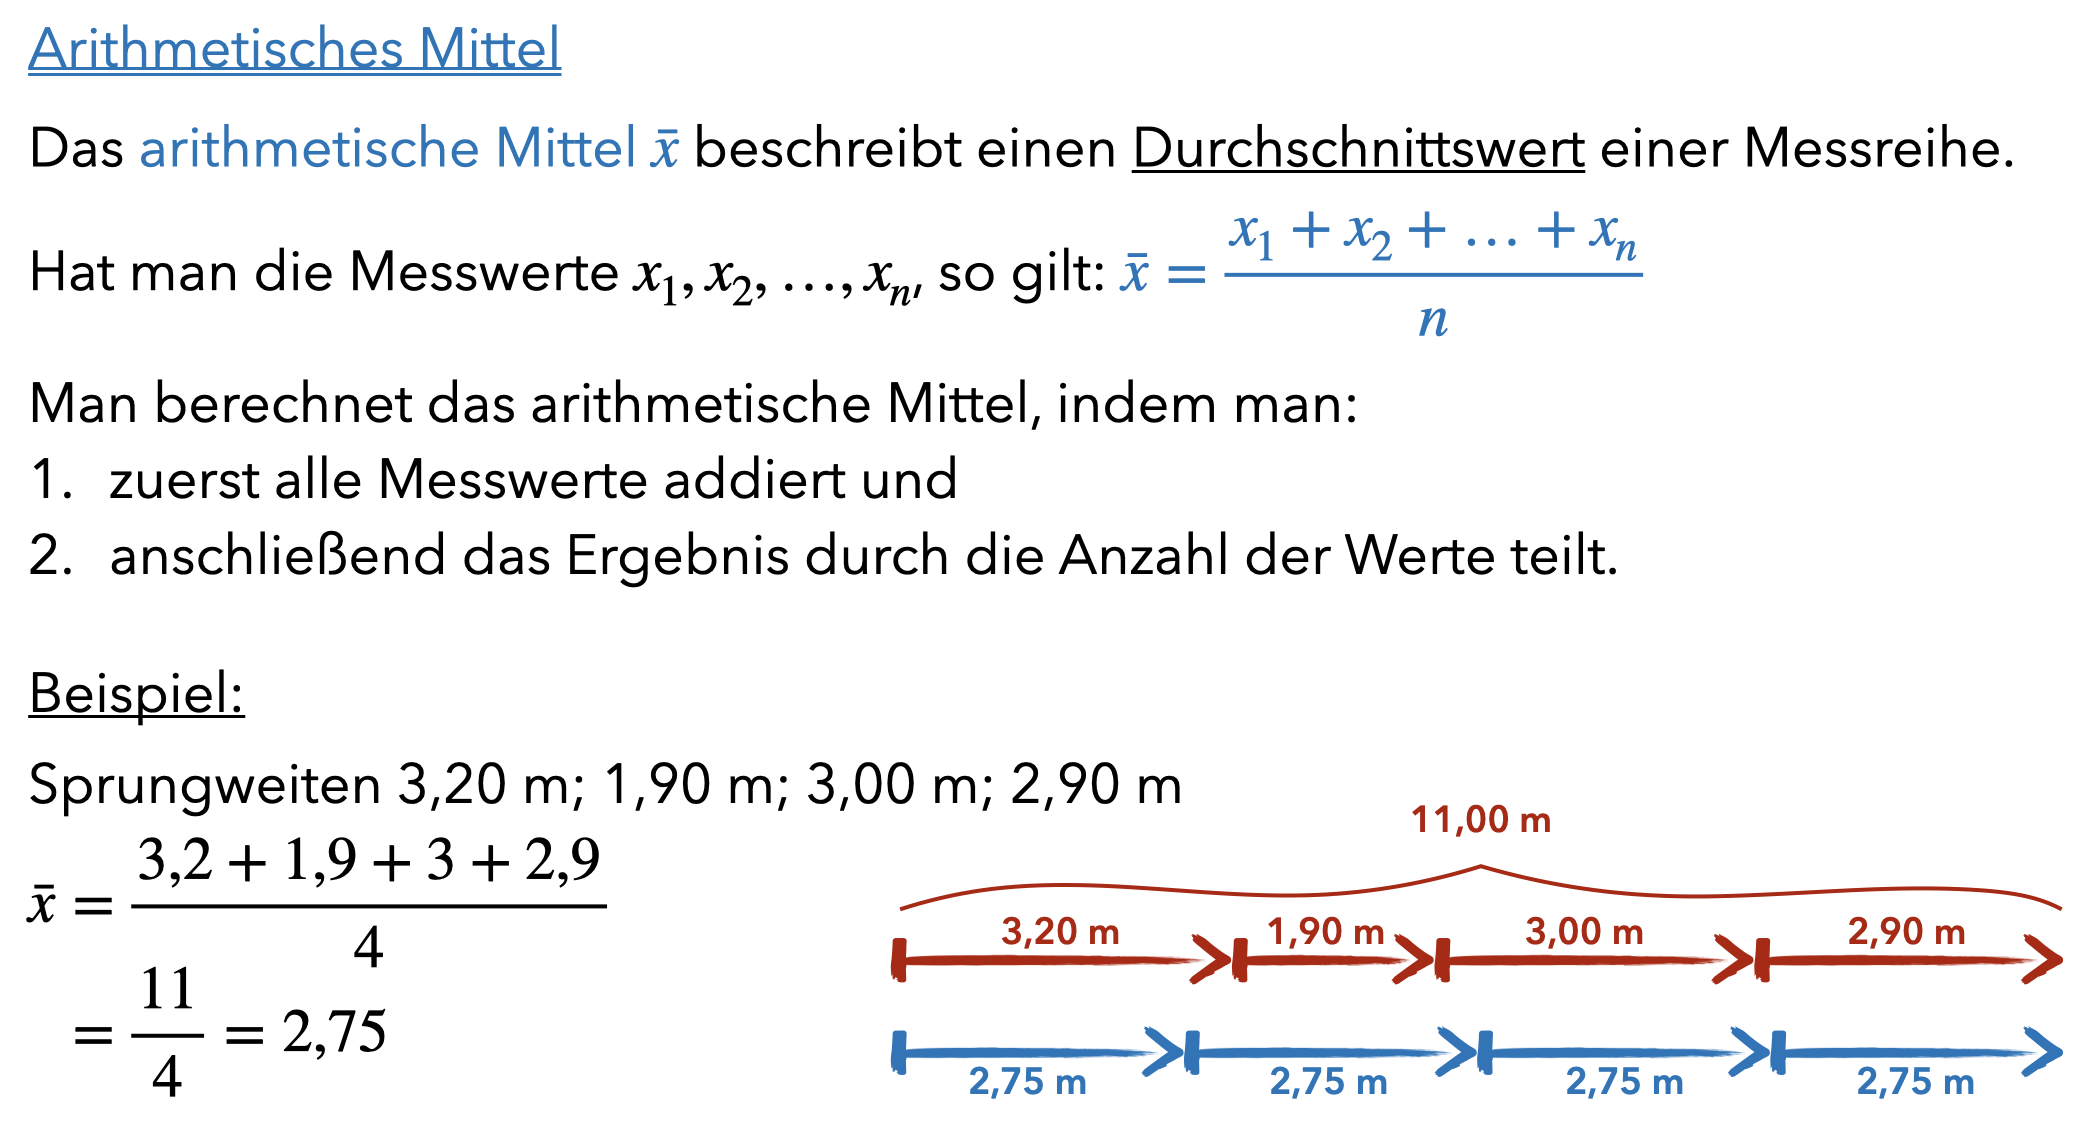
\includegraphics[width=0.9\linewidth]{pictures/B-Hefter} 

}

\caption{Hefteraufschrieb zum arithmetischen Mittel}\label{fig:Hefter}
\end{figure}

Dazu einige Kommentare:

\begin{itemize}
\tightlist
\item
  Es erfolgt zunächst eine Beschreibung, \emph{wofür} man das arithmetische Mittel verwendet und anschließend erst die formale Definition.\\
\item
  Die in der Definition enthaltene Vorgehensbeschreibung kann als \textbf{Orientierungshilfe} angesehen werden, um den Begriff des arithmetischen Mittels zu realisieren (vgl. Abschnitte @ref(orientierungsgrundöagen) und \ref{begriffe-aneignen}).\\
\item
  Das Beispiel und die Repräsentation sind Bestandteil des Aufschriebs der Definition in den Hefter, um den Schülerinnen und Schüler Anknüpfungspunkte zu bieten.
\end{itemize}

Um eine \textbf{Erstaneignung} zu ermöglichen, sollten nun einfache Identifizierungs- und Realisierungsaufgaben bearbeitet werden. Dies kann bspw. in Partnerarbeit geschehen, auch um die sprachlichen Handlungen zu unterstützen. Auch sollte die Besprechung typischer Fehler (zum Beispiel beim Eintippen in den Taschenrechner) Bestandteil der Erstaneignung sein.

\begin{itemize}
\tightlist
\item
  \emph{Berechne das arithmetisches Mittel. Beschreibe anschließend dein Vorgehen.}\\
  \emph{Person A: a) 2; 4; 3; 7; 8; b) 2,5; 1,2; 5; 7,2}\\
  \emph{Person B: a) 5; 2; 8; 3; 4; b) 3,1; 1,2; 7; 4,8}
\item
  *Erkläre, welcher Fehler, beim Berechnen des arithmetischen Mittels der Datenreihe \(10; 17; 12; 13; 20\) gemacht wurde und korrigiere ihn.
  \[\bar{x} = 10+17+12+13+20:5 = 56\]
\item
  \emph{Beschreibe, wie du beim Berechnen des arithmetischen Mittels mit dem Taschenrechner vorgehen kannst.}
\end{itemize}

\subsection{Festigung}\label{festigung-1}

Zur Festigung des arithmetischen Mittels bietet es sich an, \textbf{Aufgaben vielfältig zu variieren} (vgl. Abschnitt \ref{begriffe-festigen}) und nach dem operativen Prinzip durchzuarbeiten.\footnote{Es lohnt sich, an dieser Stelle noch einmal in die Vorlesungsunterlagen zur Einführung in die Mathematikdidaktik zu sehen.}

Speziell zum arithmetischen Mittel bietet Leuders (\citeproc{ref-Leuders2009}{2009}) hierzu eine reichhaltige Auswahl an Übungsaufgaben. Von denen müssen nun für die konkrete Unterrichtsstunde gezielt einige ausgesucht werden, ggf. auch mit Wahl- und Wahlpflichtcharakter für den differenzierenden Einsatz. Konkrete methodische Entscheidungen sind dann abhängig von der Lerngruppe zu treffen.

Sollte bereits andere Lagemaße behandelt worden sein, so bietet sich in einer Festigung auch immer ein Vergleich zwischen den Lagemaßen an. Das in Abbildung \ref{fig:ScreenshotLagemass} dargestellte \href{files/Stoffdidaktik-WiSe2223-Kap11-Lagemasse.html}{virtuelle Arbeitsmittel} ermöglicht bspw. einen \textbf{Vergleich zwischen Median und arithmetischem Mittel}.

\begin{figure}

{\centering 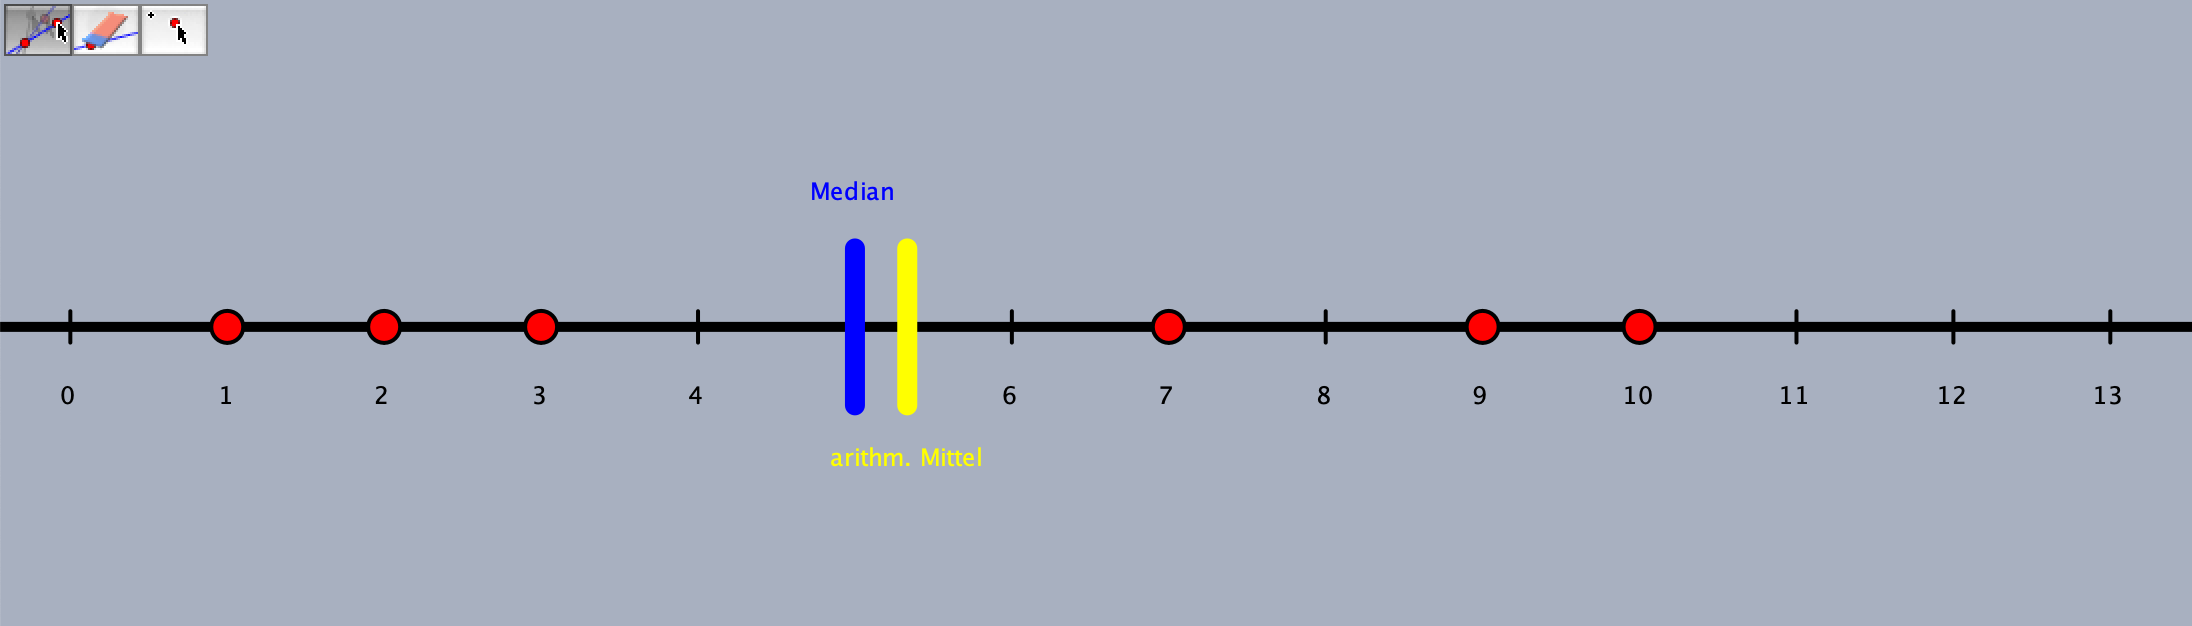
\includegraphics[width=0.75\linewidth]{pictures/B-ScreenshotLagemass} 

}

\caption{Screenshot des virtuellen Arbeitsmittels zu Lagemaßen}\label{fig:ScreenshotLagemass}
\end{figure}

Auf einer skalierten Achse sind dabei Punkte markiert und es wird das arithmetische Mittel (gelb) sowie der Median (blau) dargestellt. Die Punkte können verschoben werden und es ist möglich, neue Punkte hinzuzufügen bzw. existierende Punkte zu entfernen, wobei sich arithmetisches Mittel und Median automatisiert anpassen. Die folgenden Aufgabenstellungen zeigen exemplarisch, wie ein derartiges Arbeitsmittel genutzt werden kann, um Schülerinnen und Schüler zum operativen Durcharbeiten bezüglich dieser Lagemaße anzuregen:

\begin{itemize}
\tightlist
\item
  \emph{Verändere die Punkte so, dass Median und arithmetisches Mittel gleich sind.}
\item
  \emph{Kannst du Punkte verschieben, so dass Median oder arithmetisches Mittel unverändert bleiben? Bei welchen Punkten geht das (nicht) und warum (nicht)?}
\item
  \emph{Wie verändert sich das beobachtete Verhalten von arithmetischem Mittel und Median bei ungerader Anzahl an Punkten?}
\item
  \emph{Zeige mit dem Arbeitsmittel, dass der Median stabil gegenüber Ausreißern ist, das arithmetische Mittel jedoch nicht.}
\end{itemize}

\subsection{Handlungskontrolle}\label{handlungskontrolle-1}

Die Beurteilung der erzielten Lernergebnisse kann, bei diesem relativ übersichtlichen Lerngegenstand, durch eine kleine \textbf{Zusammenfassung am Ende der Unterrichtsstunde} erfolgen. Um hierbei auch zu prüfen, ob die gewünschten Kompetenzziele erreicht worden sind, bieten sich folgende Impulse für kurzes Plenumsgespräch an:

\begin{itemize}
\tightlist
\item
  Fasse zusammen, was wir heute neues gelernt haben.\\
\item
  Wofür benötigt man das arithmetische Mittel?
\item
  Erkläre, wie man das arithmetische Mittel berechnet.
\end{itemize}

Dabei sollte auch noch einmal ein Bezug zu den ursprünglich formulierten Lernzielen erfolgen.

Abbildung \ref{fig:Uebersicht} fasst die grundsätzliche Struktur der Unterrichtsstunde inkl. der ungefähren Zeitangabe der einzelnen noch einmal zusammen.

\begin{figure}

{\centering 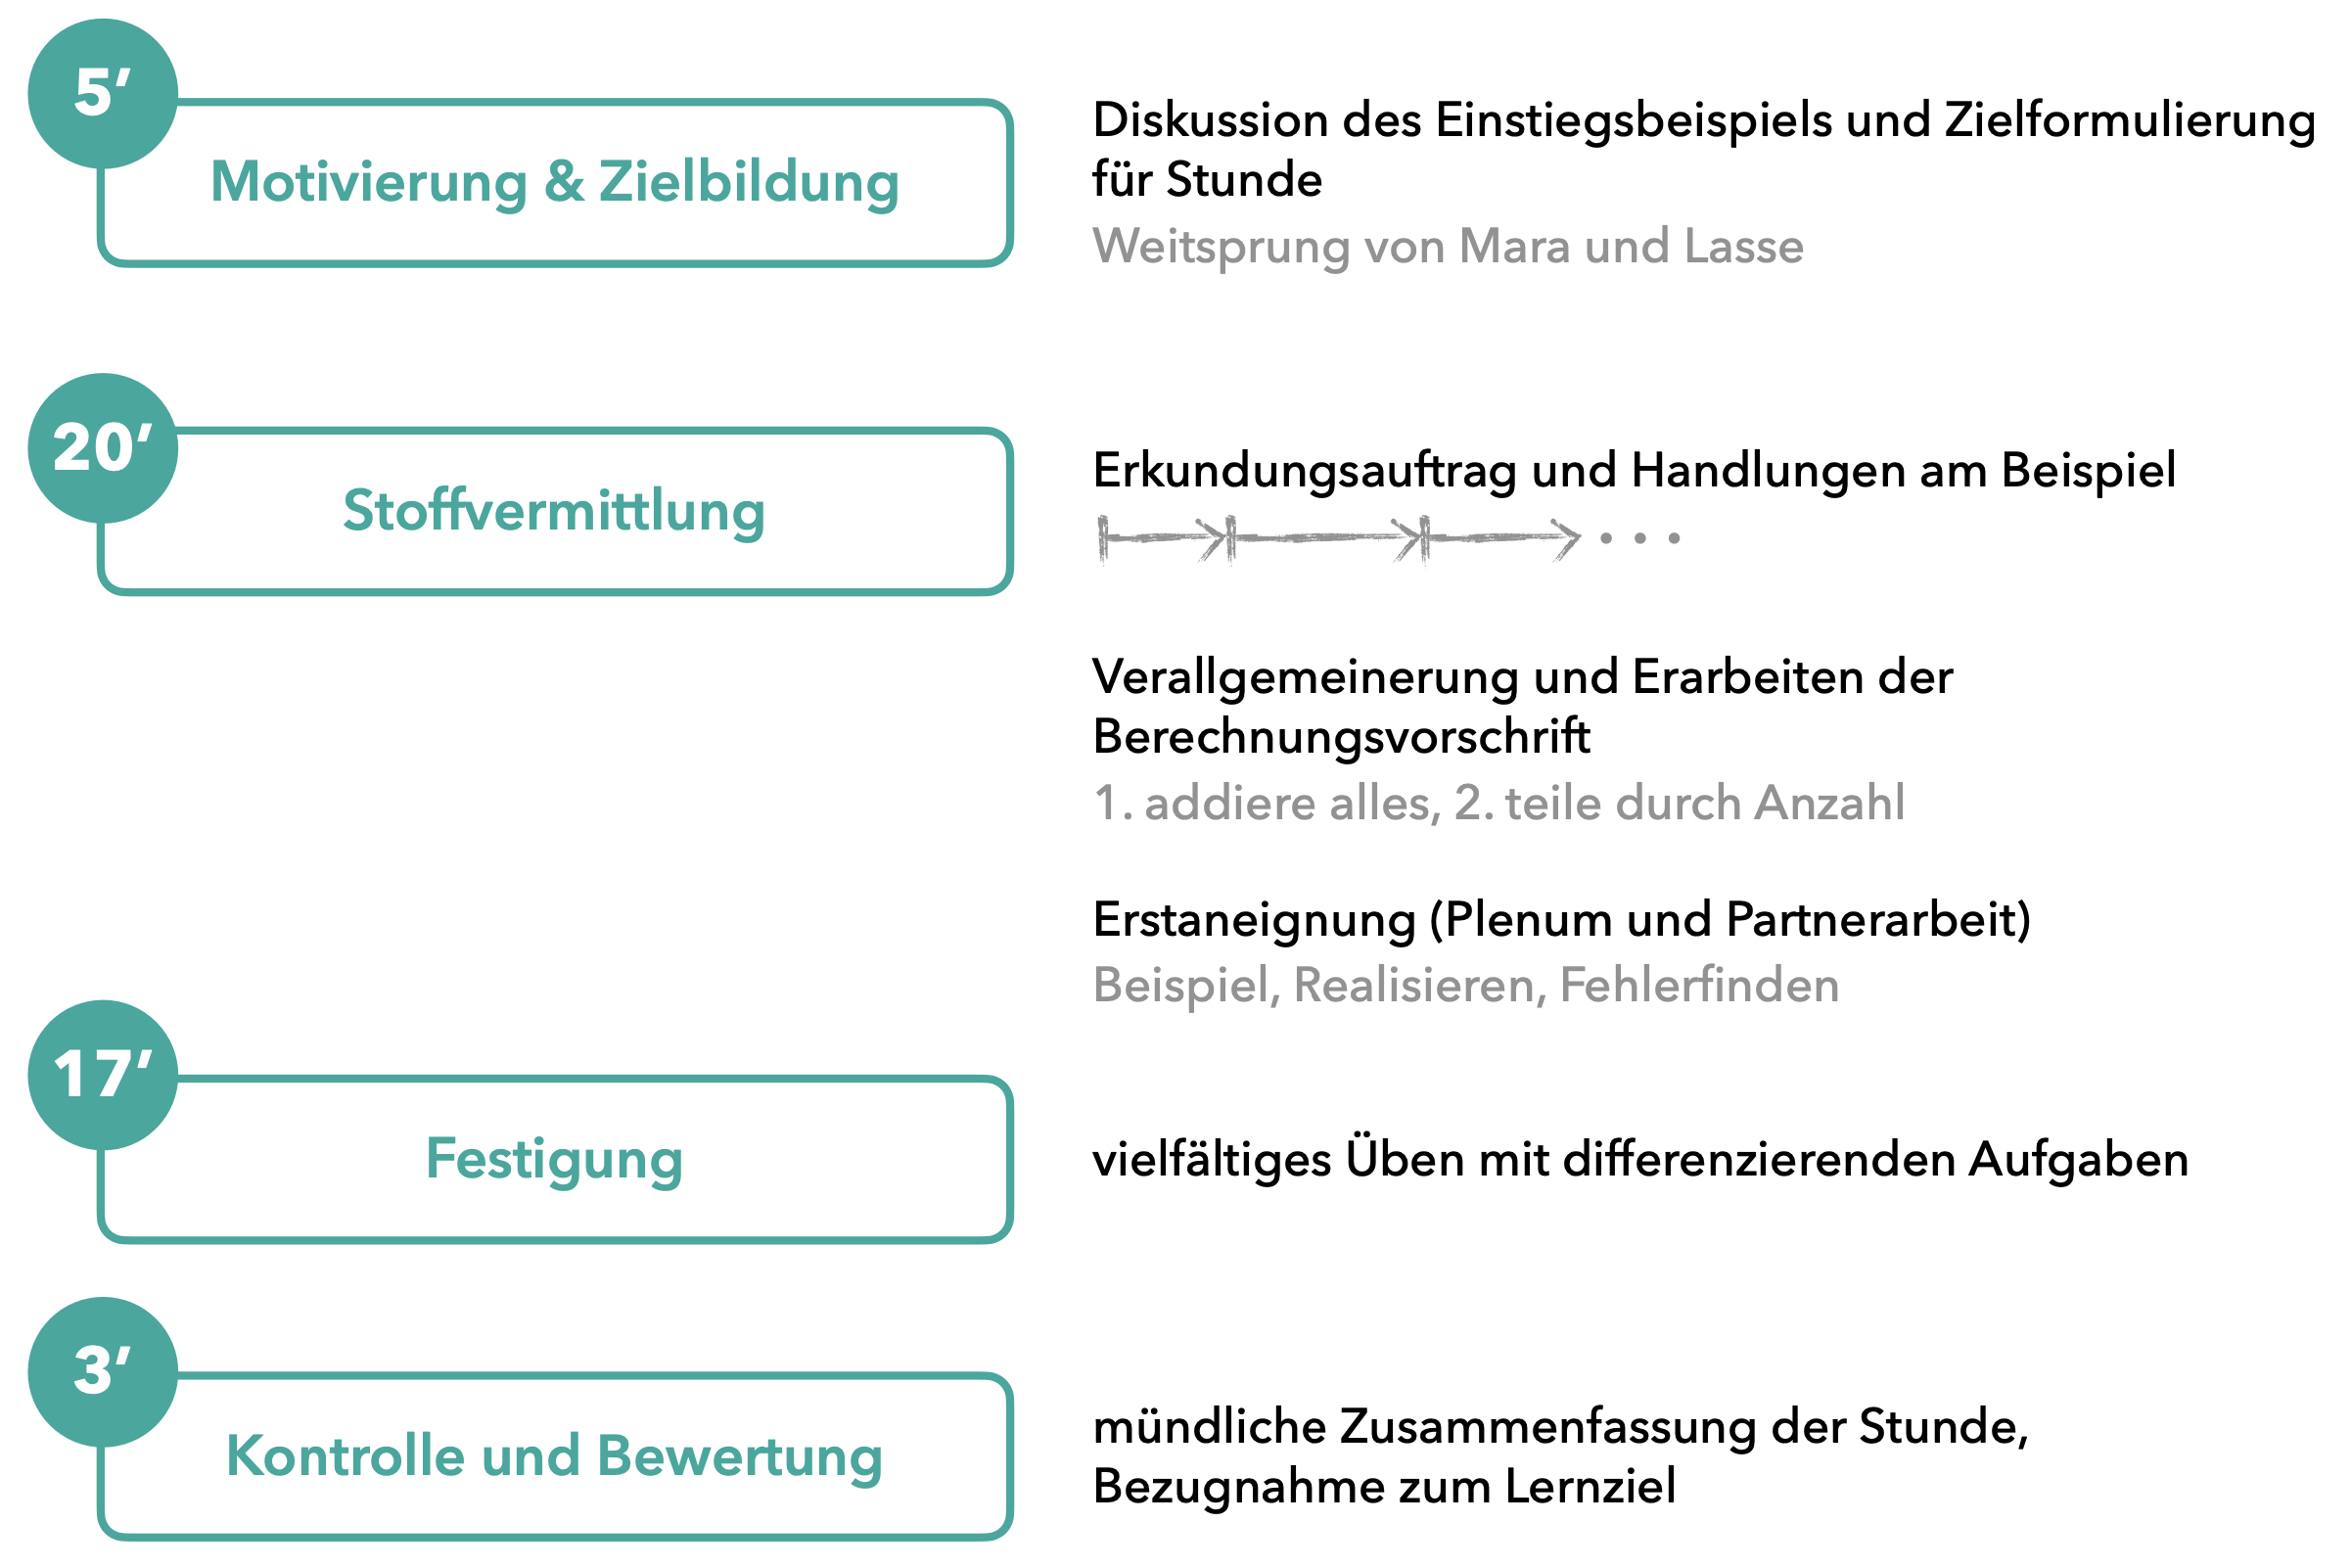
\includegraphics[width=0.9\linewidth]{pictures/B-Uebersicht} 

}

\caption{Übersicht einer Unterrichtsstunde zum arithmetischen Mittel}\label{fig:Uebersicht}
\end{figure}

\section{Zum Nachbereiten}\label{beispiel-arithmetisches-mitttel-nachbereitung}

Stellen Sie eine Sammlung geeigneter Übungsaufgaben für die Festigungsphase zum arithmetischen Mittel zusammen. Begründen Sie die Auswahl der Aufgaben mithilfe mathematikdidaktischer Theorien.

\chapter{Orientierungshilfen für Lehrhandlungen}\label{orientierungshilfen-fuxfcr-lehrhandlungen}

Dieser Anhang enthält verschiedene Orientierungshilfen für einzelne Planungs- und Durchführungshandlungen beim Lehren von Mathematik. Mehr Hinweise dazu, inwieweit Orientierungshilfen Unterstützung bieten können, finden sich in den vorherigen Kapiteln.

\section{Formale Ebene}\label{orientierungshilfe-formale-ebene}

Die Orientierungshilfe soll unterstützen, sich den Fragen der formalen Ebene einer stoffdidaktischen Analyse zu nähern.

\begin{figure}

{\centering 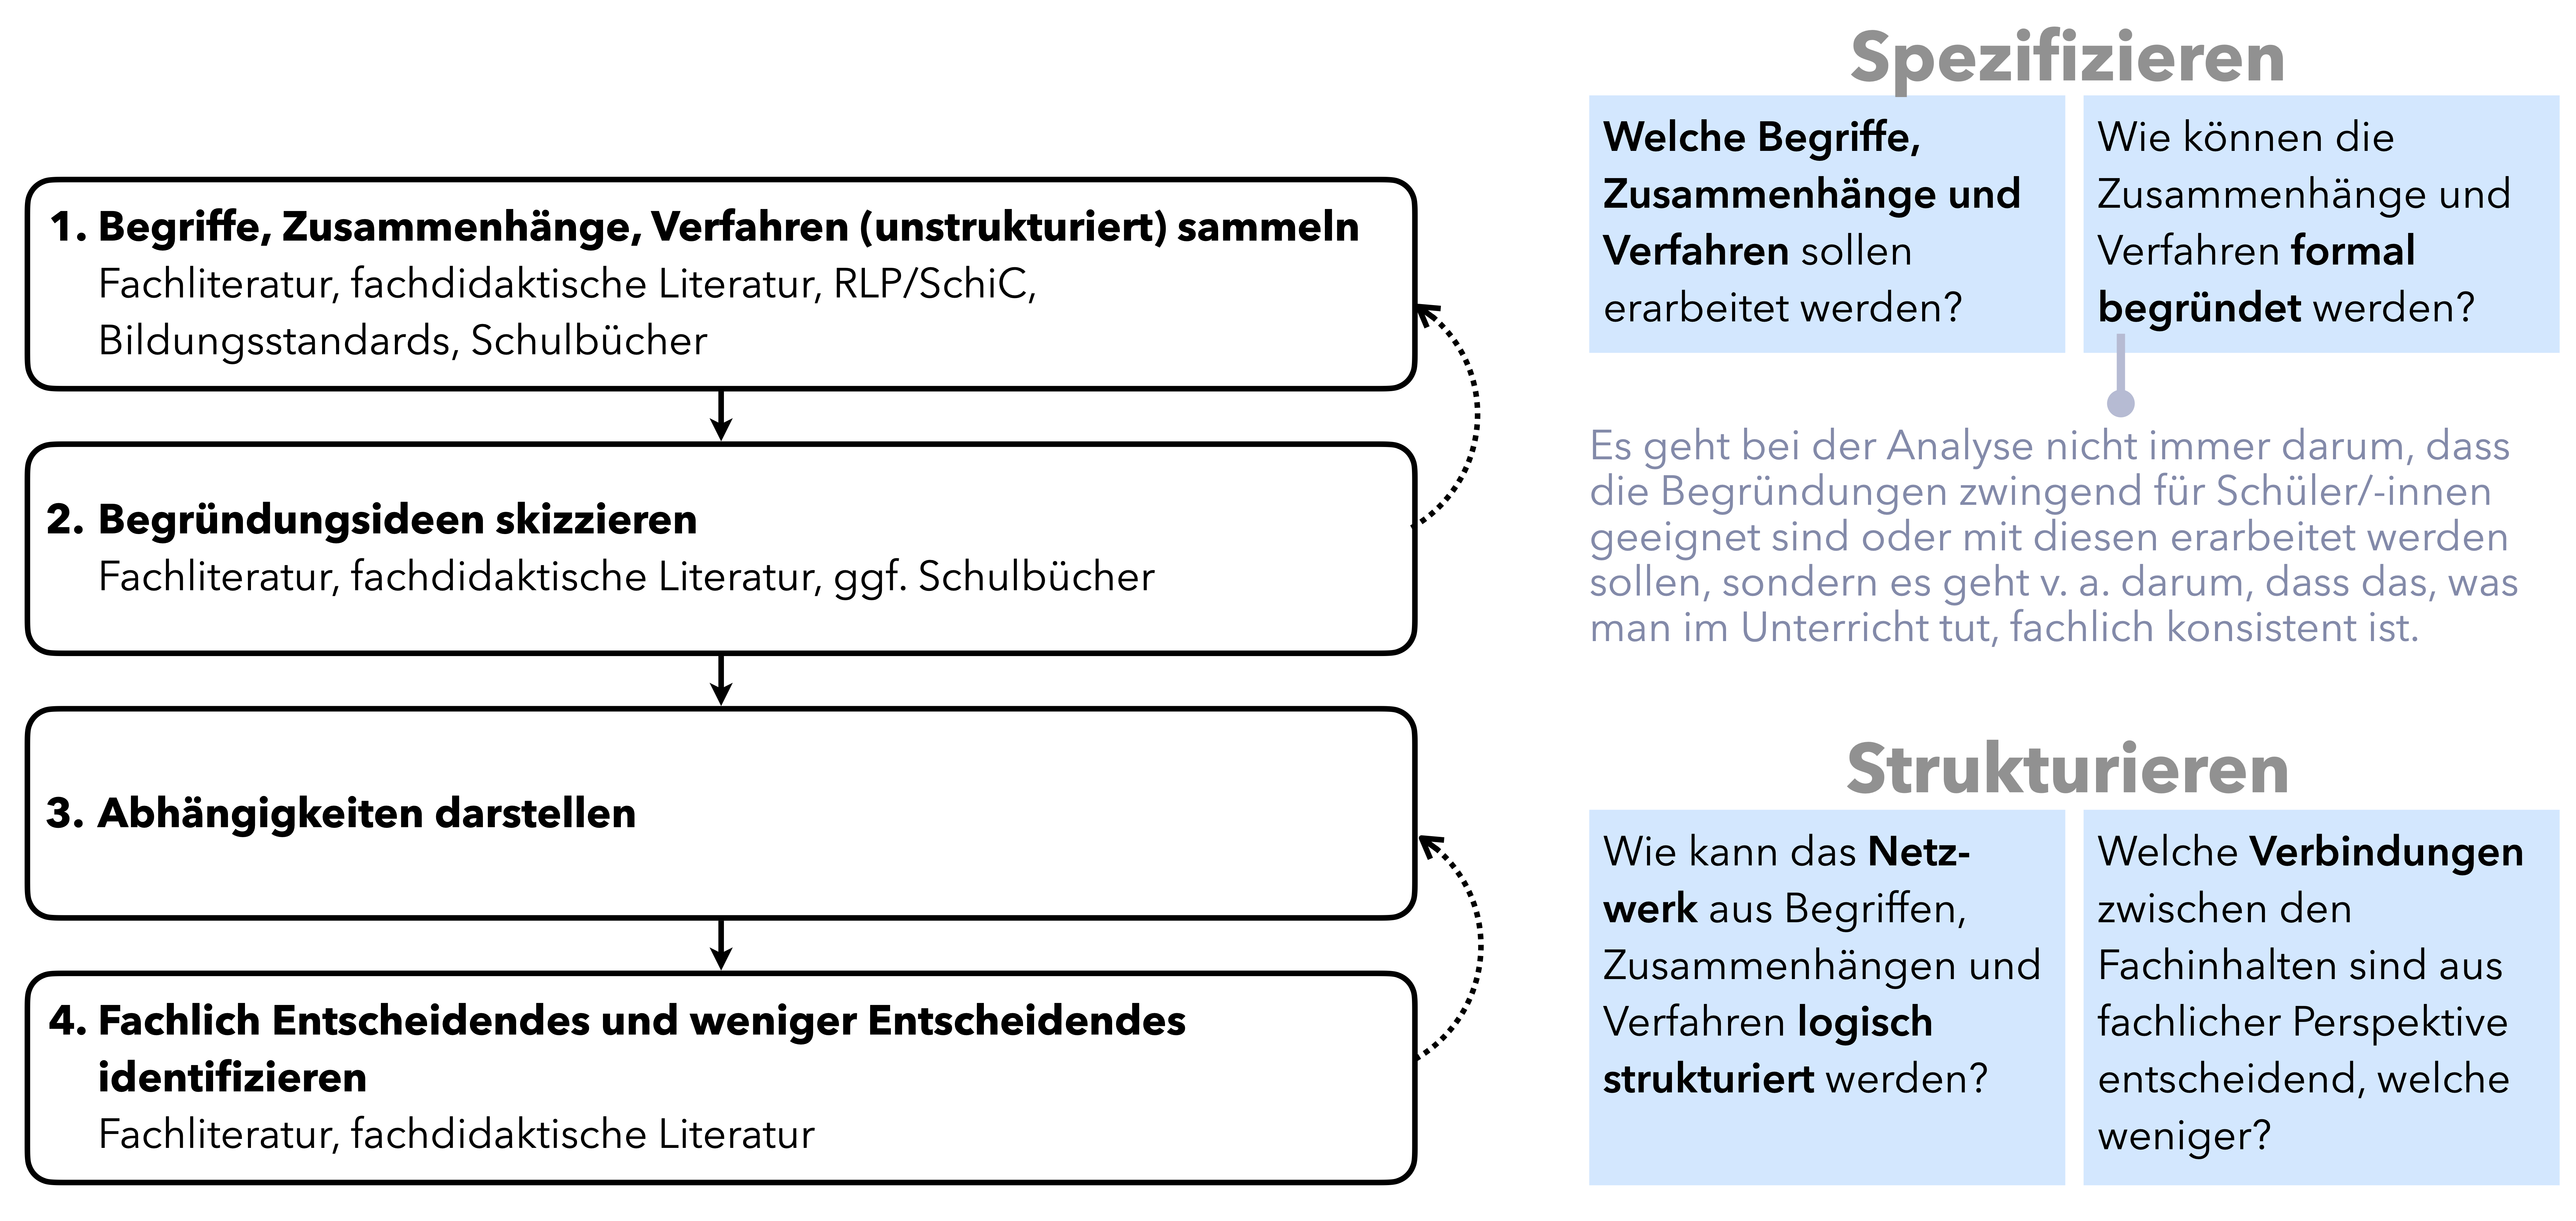
\includegraphics[width=0.9\linewidth]{pictures/C-OrientierungshilfeFormaleEbene} 

}

\caption{Orientierungshilfe zur formalen Ebene}\label{fig:OrientierungFormal}
\end{figure}

Die Übersicht kann als \href{files/Stoffdidaktik2024-OrientierungshilfeFormaleEbene.pdf}{pdf-Datei} heruntergeladen werden.

\section{Kernideen/Kernfragen finden}\label{orientierungshilfe-kernideen-finden}

Die Orientierungshilfe dient einem möglichen Vorgehen, Kernideen als das Wesen eines Lerngegenstands zu finden und diese als Kernfragen zu formulieren.

\begin{figure}

{\centering 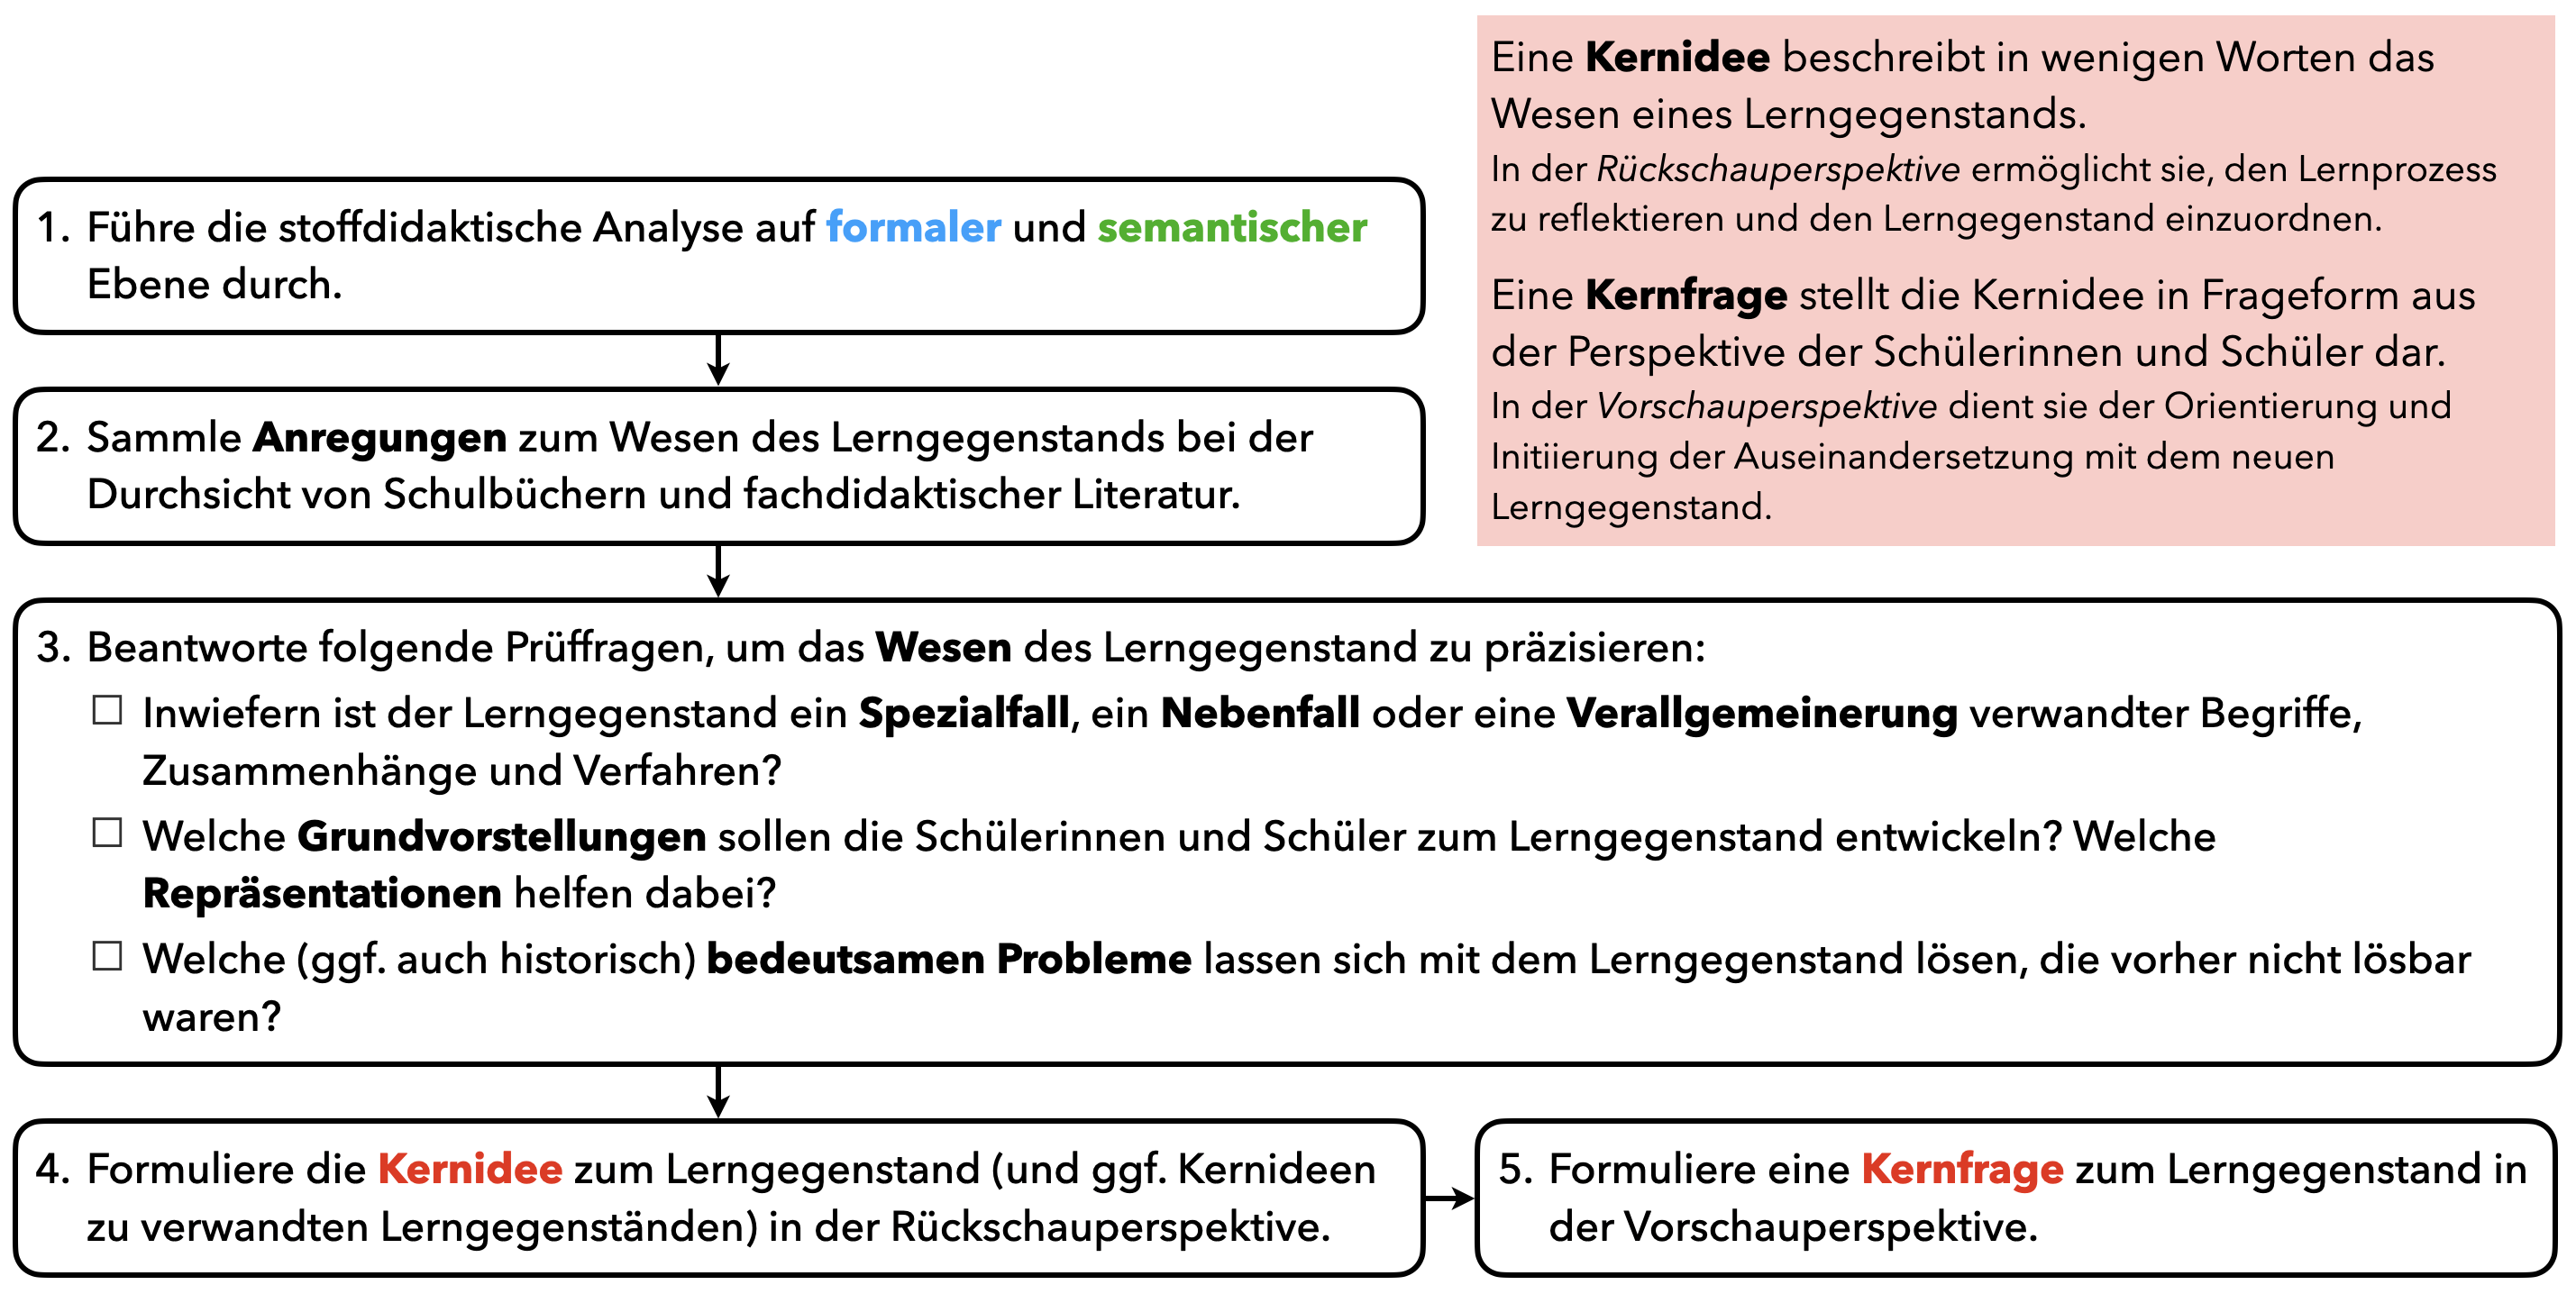
\includegraphics[width=0.9\linewidth]{pictures/C-OrientierungshilfeKernidee} 

}

\caption{Orientierungshilfe zum Finden von Kernideen und Kernfragen}\label{fig:OrientierungKernidee}
\end{figure}

Die Übersicht kann als \href{files/Stoffdidaktik2024-OrientierungshilfeKernidee.pdf}{pdf-Datei} heruntergeladen werden.

\section{Lernprozesse auslösen}\label{orientierungshilfe-lernprozesse-ausloesen}

Die Orientierungshilfe beschreibt eine Möglichkeit, die Motivierung und Zielbildung im Mathematikunterricht zu gestalten, um Lernprozesse auszulösen.

\begin{figure}

{\centering \includegraphics[width=0.9\linewidth]{pictures/C-OrientierungshilfeLernprozesseAusloesen} 

}

\caption{Orientierungshilfe zum Auslösen von Lernprozessen}\label{fig:OrientierungAusloesen}
\end{figure}

Die Übersicht kann als \href{files/Stoffdidaktik2024-OrientierungshilfeLernprozesseAusloesen.pdf}{pdf-Datei} heruntergeladen werden.

\chapter{Quellenarbeit}\label{quellenarbeit}

Um Ihre Recherche nach geeigneter fachdidaktischer Literatur zu unterstützen, sollen an dieser Stelle einige Hinweise zur Quellenarbeit gegeben werden.

\begin{itemize}
\item
  Auf der Webseite \url{https://juergen-roth.de/zeitschriften/} finden Sie eine Übersicht über \textbf{mathematikdidaktische Zeitschriften}. Als besonders geeignet für unterrichtspraktische und zugleich theoretisch fundierte Ideen soll die Zeitschrift \textbf{\emph{mathematik lehren}} empfohlen werden. Einen Themenüberblick bietet die Seite \url{https://juergen-roth.de/zeitschriften/mathematik-lehren/}, die Universitätsbibliothek Potsdam (\url{https://opac.ub.uni-potsdam.de}) verfügt über nahezu alle Ausgaben.\footnote{Bei der Suche nach dem Standort der Zeitschrift sollten Sie in der Recherche nach Zeitschriften filtern.} Auf der Webseite des Zeitschriftenverlags (\url{https://www.friedrich-verlag.de}) können Sie eine Stichwortsuche durchführen, so dass sie auch erfahren, in welchen Ausgaben einzelne Artikel enthalten sind.
\item
  Über die Webseite \url{https://eldorado.tu-dortmund.de} gelangen Sie an die \textbf{\emph{Beiträge zum Mathematikunterricht}} (BzMU). Dies sind Sammelbände, die jährlich zur Tagung der Gesellschaft für Didaktik der Mathematik (GDM) herausgegeben werden, bei der sich nahezu die komplette mathematikdidaktische Community im deutschsprachigen Raum trifft. Die Beiträge haben i.~d.~R. nur eine Länge von vier Seiten und geben einen kurzen Überblick über aktuelle Forschungsthemen. Am sinnvollsten erscheint eine Stichwortsuche über die Webseite. Die Beiträge selbst durchlaufen jedoch keinen \emph{Review-Prozess}, es kann also nicht per se eine Aussage über deren Qualität getroffen werden.
\item
  Aus dem universitätsinternen Netz bietet \url{https://link.springer.com} eine große Auswahl an \textbf{Monographien und Zeitschriften}. Einige der bei \url{https://juergen-roth.de/zeitschriften/} dargestellten Zeitschriften werden über Springer vertrieben.
\item
  Über die Seite \url{https://www.fachportal-paedagogik.de} können Sie zu den von Ihnen präferierten Stichworten Beiträge finden, die dort auch kurz zusammengefasst werden. Dies ist inbesondere für kurze \textbf{Überblicksrecherchen} sinnvoll. Die Verfügbarkeit der entsprechenden Beiträge wird dann über das Fachportal dargestellt.
\item
  Inbesondere \textbf{digital zugängliche Publikationen} lassen sich über die Webseite \url{https://www.base-search.net} recherchieren. Eine ähnliche Funktionalität, aber eher international orientiert, bietet die Seite \url{https://eric.ed.gov}.
\end{itemize}

\chapter{Vollständiges Literaturverzeichnis}\label{vollstuxe4ndiges-literaturverzeichnis}

\phantomsection\label{refs}
\begin{CSLReferences}{1}{0}
\bibitem[\citeproctext]{ref-Ableitinger2013b}
Ableitinger, C., \& Heitzer, J. (2013). Grenzwerte unterrichten. {Propädeutische} {Erfahrungen} und {Präzisierungen}. \emph{mathematik lehren}, \emph{180}, 2--10.

\bibitem[\citeproctext]{ref-Ableitinger2013}
Ableitinger, C., Kramer, J., \& Prediger, S. (Hrsg.). (2013). \emph{Zur doppelten {Diskontinuität} in der {Gymnasiallehrerbildung}: {Ansätze} zu {Verknüpfungen} der fachinhaltlichen {Ausbildung} mit schulischen {Vorerfahrungen} und {Erfordernissen}}. Springer Fachmedien Wiesbaden. \url{https://doi.org/10.1007/978-3-658-01360-8}

\bibitem[\citeproctext]{ref-Barzel2011a}
Barzel, B., \& Holzäpfel, L. (2011). Gleichungen verstehen. \emph{mathematik lehren}, \emph{169}, 2--7.

\bibitem[\citeproctext]{ref-Barzel2016}
Barzel, B., Hußmann, S., Leuders, T., \& Prediger, S. (Hrsg.). (2016). \emph{Mathewerkstatt. 9, {Schulbuch}} (Mittlerer Schulabschluss, allgemeine Ausg., 1. Aufl.). Cornelsen.

\bibitem[\citeproctext]{ref-Beutelspacher2012}
Beutelspacher, A., Danckwerts, R., Nickel, G., Spies, S., \& Wickel, G. (2012). \emph{Mathematik {Neu} {Denken}}. Vieweg+Teubner Verlag. \url{https://doi.org/10.1007/978-3-8348-8250-9}

\bibitem[\citeproctext]{ref-Boeer2014}
Böer, H., Göckel, D., Kliemann, S., Koepsell, A., Puscher, R., Schmidt, W., \& Vernay, R. (2014). \emph{Mathe live. 8, {Schülerbuch}} (1. Aufl.). Klett.

\bibitem[\citeproctext]{ref-Bruckler:2018}
Brückler, F. M. (2018). \emph{Geschichte der {Mathematik} kompakt: {Das} {Wichtigste} aus {Analysis}, {Wahrscheinlichkeitstheorie}, angewandter {Mathematik}, {Topologie} und {Mengenlehre}}. Springer Spektrum. \url{https://doi.org/10.1007/978-3-662-55574-3}

\bibitem[\citeproctext]{ref-Bruder1991}
Bruder, R. (1991). Unterrichtssituationen -- ein {Modell} für die {Aus}- und {Weiterbildung} zur {Gestaltung} von {Mathematikunterricht}. \emph{Wissenschaftliche Zeitschrift der Universität Potsdam}, \emph{35}(2), 129--134.

\bibitem[\citeproctext]{ref-Bruder2011}
Bruder, R. (2001). Mathematik lernen und behalten. \emph{Pädagogik (Weinheim)}, \emph{53}(10), 15--18.

\bibitem[\citeproctext]{ref-Bruder2008b}
Bruder, R. (2008). Üben mit {Konzept}. \emph{mathematik lehren}, \emph{147}, 4--11.

\bibitem[\citeproctext]{ref-Bruder1989}
Bruder, R., \& Brückner, A. (1989). Zur {Beschreibung} von {Schülertätigkeiten} im {Mathematikunterricht} -- ein allgemeiner {Ansatz}. \emph{Pädagogische Forschung. Wissenschaftliche Nachrichten}, \emph{30}(6), 72--82.

\bibitem[\citeproctext]{ref-Bruner:1976}
Bruner, J. S. (1976). Die {Bedeutung} der {Struktur} im {Lernprozeß}. In A. Holtmann (Hrsg.), \emph{Das sozialwissenschaftliche {Curriculum} in der {Schule}: {Neue} {Formen} und {Inhalte}} (S. 77--90). VS Verlag für Sozialwissenschaften. \url{https://doi.org/10.1007/978-3-322-85275-5}

\bibitem[\citeproctext]{ref-Danckwerts:1988}
Danckwerts, R. (1988). Linearität als organisierendes Element zentraler Inhalte der Schulmathematik. \emph{Didaktik der Mathematik}, \emph{16}(2), 149--160.

\bibitem[\citeproctext]{ref-Danckwerts2013}
Danckwerts, R. (2013). Angehende {Gymnasiallehrer}(innen) brauchen eine „{Schulmathematik} vom höheren {Standpunkt}``! In C. Ableitinger, J. Kramer, \& S. Prediger (Hrsg.), \emph{Zur doppelten {Diskontinuität} in der {Gymnasiallehrerbildung}} (S. 77--94). Springer Fachmedien Wiesbaden. \url{https://doi.org/10.1007/978-3-658-01360-8_5}

\bibitem[\citeproctext]{ref-Danckwerts2010}
Danckwerts, R., \& Vogel, D. (2010). \emph{Analysis verständlich unterrichten} (1. Aufl., 2. Nachdruck). Spektrum Akad. Verl.

\bibitem[\citeproctext]{ref-Enders2024}
Enders, J. (2024). \emph{Analysis {I} ({Lehramt}). {Skript} zur {Veranstaltung} im {WS} 2023/24} {[}Unveröffentlichtes Skript{]}.

\bibitem[\citeproctext]{ref-Etzold:2019}
Etzold, H. (2019a). \emph{Winkel-{Farm}} (Version 2) {[}App{]}. \url{https://apps.apple.com/de/app/winkel-farm/id1369585218}

\bibitem[\citeproctext]{ref-Etzold:2019Praxis4}
Etzold, H. (2019b). \emph{Winkel-{Farm} -- {Leitfaden} für {Lehrerinnen} und {Lehrer}} (Version 2). Zenodo. \url{https://doi.org/10.5281/zenodo.4747700}

\bibitem[\citeproctext]{ref-Etzold2021}
Etzold, H. (2021). \emph{Neue Zugänge zum Winkelbegriff} {[}Dissertation, Universität Potsdam{]}. \url{https://doi.org/10.25932/publishup-50418}

\bibitem[\citeproctext]{ref-Feldt-Caesar2017}
Feldt-Caesar, N. (2017). \emph{Konzeptualisierung und {Diagnose} von mathematischem {Grundwissen} und {Grundkönnen}}. Springer Fachmedien Wiesbaden. \url{https://doi.org/10.1007/978-3-658-17373-9}

\bibitem[\citeproctext]{ref-Freudenthal1973c}
Freudenthal, H. (1973a). \emph{Mathematics as an {Educational} {Task}}. Springer Netherlands. \url{https://doi.org/10.1007/978-94-010-2903-2}

\bibitem[\citeproctext]{ref-Freudenthal1973a}
Freudenthal, H. (1973c). \emph{Mathematik als pädagogische {Aufgabe}} (Bd. 1). Klett.

\bibitem[\citeproctext]{ref-Freudenthal:1973}
Freudenthal, H. (1973b). \emph{Mathematik als pädagogische {Aufgabe}} (Bd. 2). Klett.

\bibitem[\citeproctext]{ref-Gellert1986}
Gellert, W., Küstner, H., Hellwich, M., Kästner, H., \& Reichardt, H. (Hrsg.). (1986). \emph{Kleine {Enzyklopädie} {Mathematik}} (13. Aufl.). VEB Bibliographisches Institut.

\bibitem[\citeproctext]{ref-Giest2016a}
Giest, H. (2016). Kulturhistorische {Didaktik} und {Bildungstheorie}. \emph{Tätigkeitstheorie. Journal für tätigkeitstheoretische Forschung in Deutschland}, \emph{14}, 24--48. \url{http://www.ich-sciences.de/media/journal/Ausgabe_14/heft_14.pdf}

\bibitem[\citeproctext]{ref-Giest2004a}
Giest, H., \& Lompscher, J. (2004). Tätigkeitstheoretische Überlegungen zu einer neuen {Lernkultur}. \emph{Sitzungsberichte der Leibniz-Sozietät}, \emph{72}, 101--123. \url{https://leibnizsozietaet.de/wp-content/uploads/2012/11/07_giest.pdf}

\bibitem[\citeproctext]{ref-Giest2006}
Giest, H., \& Lompscher, J. (2006). \emph{Lerntätigkeit -- {Lernen} aus kultur-historischer {Perspektive}. {Ein} {Beitrag} zur {Entwicklung} einer neuen {Lernkultur} im {Unterricht}}. Lehmanns Media.

\bibitem[\citeproctext]{ref-Greefrath2016}
Greefrath, G., Oldenburg, R., Siller, H.-S., Ulm, V., \& Weigand, H.-G. (2016). \emph{Didaktik der {Analysis}. {Aspekte} und {Grundvorstellungen} zentraler {Begriffe}} (F. Padberg \& A. Büchter, Hrsg.; 4. Aufl.). Springer Spektrum. \url{https://doi.org/10.1007/978-3-662-48877-5}

\bibitem[\citeproctext]{ref-Hefendehl-Hebeker:2016}
Hefendehl-Hebeker, L. (2016). Subject-matter didactics in {German} traditions: {Early} historical developments. \emph{Journal für Mathematik-Didaktik}, \emph{37}(S1), 11--31. \url{https://doi.org/10.1007/s13138-016-0103-7}

\bibitem[\citeproctext]{ref-Heinrich2007}
Heinrich, R. (2007). Grafikfähige {Taschencomputer} in zentralen {Prüfungen}. In \emph{Beiträge zum {Mathematikunterricht} 2007, 41. {Jahrestagung} der {Gesellschaft} für {Didaktik} der {Mathematik} vom 25.3. bis 30.3.2007 in {Berlin}}. \url{https://doi.org/10.17877/DE290R-6165}

\bibitem[\citeproctext]{ref-Henn2015}
Henn, H.-W., \& Filler, A. (2015). \emph{Didaktik der {Analytischen} {Geometrie} und {Linearen} {Algebra}: {Algebraisch} verstehen -- {Geometrisch} veranschaulichen und anwenden}. Springer Spektrum.

\bibitem[\citeproctext]{ref-Hussmann:2016}
Hußmann, S., \& Prediger, S. (2016). Specifying and Structuring Mathematical Topics: A Four-Level Approach for Combining Formal, Semantic, Concrete, and Empirical Levels Exemplified for Exponential Growth. \emph{Journal für Mathematik-Didaktik}, \emph{37}(S1), 33--67. \url{https://doi.org/10.1007/s13138-016-0102-8}

\bibitem[\citeproctext]{ref-Hussmann:2016a}
Hußmann, S., Rezat, S., \& Sträßer, R. (2016). Subject {Matter} {Didactics} in {Mathematics} {Education}. \emph{Journal für Mathematik-Didaktik}, \emph{37}(S1), 1--9. \url{https://doi.org/10.1007/s13138-016-0105-5}

\bibitem[\citeproctext]{ref-Jahnke:2010}
Jahnke, T. (2010). Vom mählichen {Verschwinden} des {Fachs} aus der {Mathematikdidaktik}. \emph{GDM-Mitteilungen 89}, 21--24. \url{https://ojs.didaktik-der-mathematik.de/index.php/mgdm/article/view/559/550}

\bibitem[\citeproctext]{ref-Klein1925}
Klein, F. (1925). \emph{Elementarmathematik vom {Höheren} {Standpunkte} aus {II}. {Geometrie}}. Springer Berlin Heidelberg. \url{https://doi.org/10.1007/978-3-642-90852-1}

\bibitem[\citeproctext]{ref-Klein1955}
Klein, F. (1955). \emph{Elementarmathematik vom {Höheren} {Standpunkte} aus {III}. {Präzisions}- und {Approximationsmathematik}} (C. H. Müller, Hrsg.). Springer Berlin Heidelberg. \url{https://doi.org/10.1007/978-3-662-00246-9}

\bibitem[\citeproctext]{ref-Klein1967}
Klein, F. (1967). \emph{Elementarmathematik vom {Höheren} {Standpunkte} aus {I}. {Arithmetik}, {Algebra}, {Analysis}}. Springer Berlin Heidelberg. \url{https://doi.org/10.1007/978-3-662-11652-4}

\bibitem[\citeproctext]{ref-Kortenkamp2007}
Kortenkamp, U. (2007). {CAS} und {DGS} im {Dialog} -- oder: {Wieviel} {CAS} braucht der {Mensch}? In \emph{Beiträge zum {Mathematikunterricht} 2007, 41. {Jahrestagung} der {Gesellschaft} für {Didaktik} der {Mathematik} vom 25.3. bis 30.3.2007 in {Berlin}}. \url{https://doi.org/10.17877/DE290R-6158}

\bibitem[\citeproctext]{ref-Krainer:1989}
Krainer, K. (1989). \emph{Lebendige {Geometrie}. Überlegungen zu einem integrativen {Verständnis} von {Geometrieunterricht} anhand des {Winkelbegriffs}} {[}Dissertation{]}. Alpen-Adria-Universität Klagenfurt.

\bibitem[\citeproctext]{ref-Krauthausen:2018}
Krauthausen, G. (2018). \emph{Einführung in die {Mathematikdidaktik}} (F. Padberg \& A. Büchter, Hrsg.; Mathematik Primarstufe und Sekundarstufe I + II). Springer Spektrum. \url{https://doi.org/10.1007/978-3-662-54692-5}

\bibitem[\citeproctext]{ref-Kruger2015}
Krüger, K., Sill, H.-D., \& Sikora, C. (2015). \emph{Didaktik der {Stochastik} in der {Sekundarstufe} {I}}. Springer Berlin Heidelberg. \url{https://doi.org/10.1007/978-3-662-43355-3}

\bibitem[\citeproctext]{ref-Lambert:2012}
Lambert, A. (2012). \emph{Gedanken zum aktuellen {Kompetenzbegriff} für den ({Mathematik}-)unterricht} {[}Vortrag{]}. Eingangsstatement zur Podiumsdiskussion im Rahmen des 3. Fachdidaktischen Kolloquiums an der Universität des Saarlandes, Saarbrücken. \url{https://www.uni-saarland.de/fileadmin/upload/einrichtung/zfl/PDF_Fachdidaktik/PDF_Kolloquium_FD/Kompetenzbegriff_für_den_Mathematikunterricht_Statement_mit_Folien.pdf}

\bibitem[\citeproctext]{ref-Leuders2009}
Leuders, T. (2009). Intelligent üben und {Mathematik} erleben. In T. Leuders, L. Hefendehl-Hebeker, \& H.-G. Weigand (Hrsg.), \emph{Mathemagische {Momente}} (S. 130--143). Cornelsen. \url{https://home.ph-freiburg.de/leudersfr/preprint/2009_leuders_intelligent_ueben_mathemagische_momente.pdf}

\bibitem[\citeproctext]{ref-Leuders2011}
Leuders, T., Hußmann, S., Barzel, B., \& Prediger, S. (2011). Das macht {Sinn}! {Sinnstiftung} mit {Kontexten} und {Kernideen}. \emph{Praxis der Mathematik in der Schule}, \emph{53}(37), 2--9. \url{https://www.researchgate.net/publication/233978329}

\bibitem[\citeproctext]{ref-Lompscher1985a}
Lompscher, J. (1983). Die {Ausbildung} von {Lernhandlungen}. In J. Lompscher (Hrsg.), \emph{Persönlichkeitsentwicklung in der {Lerntätigkeit}} (S. 53--78). Volk und Wissen.

\bibitem[\citeproctext]{ref-Lompscher1985b}
Lompscher, J. (1985). Die {Lerntätigkeit} als dominierende {Tätigkeit} des jüngeren {Schülers}. In J. Lompscher (Hrsg.), \emph{Persönlichkeitsentwicklung in der {Lerntätigkeit}} (S. 23--52). Volk und Wissen.

\bibitem[\citeproctext]{ref-Lompscher1996}
Lompscher, J. (1996). \emph{Aufsteigen vom {Abstrakten} zum {Konkreten} - {Lernen} und {Lehren} in {Zonen} der nächsten {Entwicklung}}. \url{https://publishup.uni-potsdam.de/opus4-ubp/frontdoor/deliver/index/docId/444/file/AUFSTEIG.pdf}

\bibitem[\citeproctext]{ref-Mienert2011}
Mienert, M., \& Pitcher, S. (2011). \emph{Pädagogische {Psychologie}}. VS Verlag für Sozialwissenschaften. \url{https://doi.org/10.1007/978-3-531-92095-5}

\bibitem[\citeproctext]{ref-MinisteriumfurBildungJugendundSportdesLandesBrandenburg2022a}
Ministerium für Bildung, Jugend und Sport des Landes Brandenburg (Hrsg.). (2022a). \emph{Anlage zum {Rahmenlehrplan} für die gymnasiale {Oberstufe}. {Teil} {C}. {Mathematik}}. \url{https://bildungsserver.berlin-brandenburg.de/fileadmin/bbb/unterricht/rahmenlehrplaene/gymnasiale_oberstufe/curricula/2022/Teil_C_RLP_GOST_2022_Mathematik_Anlage_OHiMi.pdf}

\bibitem[\citeproctext]{ref-MinisteriumfurBildungJugendundSportdesLandesBrandenburg2022}
Ministerium für Bildung, Jugend und Sport des Landes Brandenburg (Hrsg.). (2022b). \emph{Rahmenlehrplan für die gymnasiale {Oberstufe}. {Teil} {C}. {Mathematik}}. \url{https://bildungsserver.berlin-brandenburg.de/fileadmin/bbb/unterricht/rahmenlehrplaene/gymnasiale_oberstufe/curricula/2022/Teil_C_RLP_GOST_2022_Mathematik.pdf}

\bibitem[\citeproctext]{ref-MinisteriumfuerBildungJugendundSportdesLandesBrandenburg2023}
Ministerium für Bildung, Jugend und Sport des Landes Brandenburg (Hrsg.). (2023). \emph{Rahmenlehrplan {Brandenburg}. {Teil} {C}, {Mathematik}, {Jahrgangsstufen} 1~--~10}. \url{https://bildungsserver.berlin-brandenburg.de/fileadmin/bbb/unterricht/rahmenlehrplaene/Rahmenlehrplanprojekt/amtliche_Fassung/getrennt_2023/BB_RLP_2023_Teil_C_Ma_GenF_1.pdf}

\bibitem[\citeproctext]{ref-Mitchelmore:1990}
Mitchelmore, M. (1990). Psychologische und mathematische Schwierigkeiten beim Lernen des Winkelbegriffs. \emph{mathematica didactica}, \emph{13}, 19--37.

\bibitem[\citeproctext]{ref-Mitchelmore:1998}
Mitchelmore, M., \& White, P. (1998). Development of {Angle} {Concepts}: {A} {Framework} for {Research}. \emph{Mathematics Education Research Journal}, \emph{10}(3), 4--27.

\bibitem[\citeproctext]{ref-Padberg2021}
Padberg, F., \& Benz, C. (2021). \emph{Didaktik der {Arithmetik}: fundiert, vielseitig, praxisnah} (5., überarbeitete Aufl.). Springer Spektrum.

\bibitem[\citeproctext]{ref-Padberg:2017}
Padberg, F., \& Wartha, S. (2017). \emph{Didaktik der {Bruchrechnung}} (5. Aufl.). Springer Spektrum. \url{https://doi.org/10.1007/978-3-662-52969-0}

\bibitem[\citeproctext]{ref-Reinhold2023}
Reinhold, F., Walter, D., \& Weigand, H.-G. (2023). Digitale {Medien}. In R. Bruder, A. Büchter, H. Gasteiger, B. Schmidt-Thieme, \& H.-G. Weigand (Hrsg.), \emph{Handbuch der {Mathematikdidaktik}} (S. 523--559). Springer Berlin Heidelberg. \url{https://doi.org/10.1007/978-3-662-66604-3_17}

\bibitem[\citeproctext]{ref-Reitz-Koncebovski2018}
Reitz-Koncebovski, K., Kortenkamp, U., \& Goral, J. (2018). Gestaltungsprinzipien für fachwissenschaftliche {Einführungsveranstaltungen}. In A. Borowski, A. Ehlert, \& H. Prechtl (Hrsg.), \emph{{PSI}-{Potsdam}. {Ergebnisbericht} zu den {Aktivitäten} im {Rahmen} der {Qualitätsoffensive} {Lehrerbildung} (2015-2018)} (S. 175--188). Universitätsverlag Potsdam. \url{https://nbn-resolving.org/urn:nbn:de:kobv:517-opus4-420301}

\bibitem[\citeproctext]{ref-Rembowski2015}
Rembowski, V. (2015). \emph{Eine semiotische und philosophisch-psychologische {Perspektive} auf {Begriffsbildung} im {Geometrieunterricht}. {Begriffsfeld}, {Begriffsbild} und {Begriffskonvention} und ihre {Implikationen} auf {Grundvorstellungen}} {[}Dissertation, Universität des Saarlandes{]}. \url{https://doi.org/10.22028/D291-26661}

\bibitem[\citeproctext]{ref-Richter2016}
Richter, K., \& Bruder, R. (2016). Das {Tätigkeitskonzept} als {Analyseinstrument} für technologiegestützte {Lernprozesse} im {Fach} {Mathematik}. In G. Heintz, H.-J. Elschenbroich, G. Pinkernell, \& F. Schacht (Hrsg.), \emph{Digitale {Werkzeuge} für den {Mathematikunterricht}: {Festschrift} für {Hans}-{Jürgen} {Elschenbroich}} (1. Auflage, S. 188--214). Verlag Klaus Seeberger.

\bibitem[\citeproctext]{ref-Salle2021}
Salle, A., \& Clüver, T. (2021). Herleitung von {Grundvorstellungen} als normative {Leitlinien} -- {Beschreibung} eines theoriebasierten {Verfahrensrahmens}. \emph{Journal für Mathematik-Didaktik}. \url{https://doi.org/10.1007/s13138-021-00184-5}

\bibitem[\citeproctext]{ref-Schecker2018}
Schecker, H., Wilhelm, T., Hopf, M., \& Duit, R. (Hrsg.). (2018). \emph{Schülervorstellungen und {Physikunterricht}: {Ein} {Lehrbuch} für {Studium}, {Referendariat} und {Unterrichtspraxis}}. Springer Berlin Heidelberg. \url{https://doi.org/10.1007/978-3-662-57270-2}

\bibitem[\citeproctext]{ref-Schubert:2011}
Schubert, S., \& Schwill, A. (2011). \emph{Didaktik der {Informatik}} (2. Aufl). Spektrum, Akad. Verl. \url{https://doi.org/10.1007/978-3-8274-2653-6}

\bibitem[\citeproctext]{ref-Schupp:2016}
Schupp, H. (2016). Gedanken zum „{Stoff}`` und zur „{Stoffdidaktik}`` sowie zu ihrer {Bedeutung} für die {Qualität} des {Mathematikunterrichts}. \emph{Mathematische Semesterberichte}, \emph{63}(1), 69--92. \url{https://doi.org/10.1007/s00591-016-0159-y}

\bibitem[\citeproctext]{ref-Schwill:1994}
Schwill, A. (1994). \emph{Fundamentale {Ideen} in {Mathematik} und {Informatik}}. Herbsttagung des Arbeitskreises Mathematikunterricht und Informatik, Wolfenbüttel. \url{http://www.informatikdidaktik.de/didaktik/Forschung/Wolfenbuettel94.pdf}

\bibitem[\citeproctext]{ref-KMK:2012}
Sekretariat der Ständigen Konferenz der Kultusminister der Länder in der Bundesrepublik Deutschland. (2012). \emph{Bildungsstandards im {Fach} {Mathematik} für die {Allgemeine} {Hochschulreife}. (Beschluss der Kultusministerkonferenz vom 18.10.2012)}. \url{https://www.kmk.org/fileadmin/Dateien/veroeffentlichungen_beschluesse/2012/2012_10_18-Bildungsstandards-Mathe-Abi.pdf}

\bibitem[\citeproctext]{ref-SekretariatderStandigenKonferenzderKultusministerderLanderinderBundesrepublikDeutschland2022}
Sekretariat der Ständigen Konferenz der Kultusminister der Länder in der Bundesrepublik Deutschland. (2022a). \emph{Bildungsstandards für das {Fach} {Mathematik} {Erster} {Schulabschluss} ({ESA}) und {Mittlerer} {Schulabschluss} ({MSA}). ({Beschluss} der {Kultusministerkonferenz} vom 15.10.2004 und vom 04.12.2003, i.d.{F}. vom 23.06.2022)}. \url{https://www.kmk.org/fileadmin/Dateien/veroeffentlichungen_beschluesse/2022/2022_06_23-Bista-ESA-MSA-Mathe.pdf}

\bibitem[\citeproctext]{ref-SekretariatderStandigenKonferenzderKultusministerderLanderinderBundesrepublikDeutschland2022a}
Sekretariat der Ständigen Konferenz der Kultusminister der Länder in der Bundesrepublik Deutschland. (2022b). \emph{Bildungsstandards für das {Fach} {Mathematik} {Primarbereich}. ({Beschluss} der {Kultusministerkonferenz} vom 15.10.2004, i.d.{F}. vom 23.06.2022)}. \url{https://www.kmk.org/fileadmin/Dateien/veroeffentlichungen_beschluesse/2022/2022_06_23-Bista-Primarbereich-Mathe.pdf}

\bibitem[\citeproctext]{ref-Steinhofel1988}
Steinhöfel, W., Reichold, K., \& Frenzel, L. (1988). \emph{Zur {Gestaltung} typischer {Unterrichtssituationen} im {Mathematikunterricht}}. Ministerium für Volksbildung.

\bibitem[\citeproctext]{ref-Strehl:1983}
Strehl, R. (1983). Anschauliche {Vorstellung} und mathematische {Theorie} beim {Winkelbegriff}. \emph{mathematica didactica}, \emph{6}, 129--146.

\bibitem[\citeproctext]{ref-Taylor:1715}
Taylor, B. (1715). \emph{Linear perspective}. printed for R. Knaplock at the Bishop's-Head in St. Paul's Church-Yard. \url{https://nl.sub.uni-goettingen.de/id/0590700700}

\bibitem[\citeproctext]{ref-Thiel-Schneider2018}
Thiel-Schneider, A. (2018). \emph{Zum {Begriff} des exponentiellen {Wachstums}}. Springer Fachmedien Wiesbaden. \url{https://doi.org/10.1007/978-3-658-21895-9}

\bibitem[\citeproctext]{ref-Tietze:2000a}
Tietze, U.-P., Klika, M., \& Wolpers, H. (Hrsg.). (2000a). \emph{Mathematikunterricht in der {Sekundarstufe} {II}. {Band} 1: {Fachdidaktische} {Grundfragen}, {Didaktik} der {Analysis}} (2. Aufl.). Vieweg+Teubner Verlag. \url{https://doi.org/10.1007/978-3-322-90568-0}

\bibitem[\citeproctext]{ref-Tietze:2000}
Tietze, U.-P., Klika, M., \& Wolpers, H. (Hrsg.). (2000b). \emph{Mathematikunterricht in der {Sekundarstufe} {II}. {Band} 2: {Didaktik} der {Analytischen} {Geometrie} und {Linearen} {Algebra}}. Vieweg+Teubner Verlag. \url{https://doi.org/10.1007/978-3-322-86479-6}

\bibitem[\citeproctext]{ref-Tietze:2002}
Tietze, U.-P., Klika, M., \& Wolpers, H. (Hrsg.). (2002). \emph{Mathematikunterricht in der {Sekundarstufe} {II}. {Band} 3: {Didaktik} der {Stochastik}}. Vieweg+Teubner Verlag. \url{https://doi.org/10.1007/978-3-322-83144-6}

\bibitem[\citeproctext]{ref-vandenHeuvel-Panhuizen2003}
van den Heuvel-Panhuizen, M. (2003). The didactical use of models in realistic mathematics education: {An} example from a longitudinal trajectory on percentage. \emph{Educational Studies in Mathematics}, \emph{54}, 9--35. \url{https://doi.org/10.1023/B:EDUC.0000005212.03219.dc}

\bibitem[\citeproctext]{ref-Vohns:2000}
Vohns, A. (2000). \emph{Das {Messen} als fundamentale {Idee}} {[}1. Staatsexamensarbeit, Universität-Gesamthochschule Siegen{]}. \url{https://wwwu.aau.at/avohns/pdf/messen.pdf}

\bibitem[\citeproctext]{ref-Vollrath2012}
Vollrath, H.-J., \& Roth, J. (2012). \emph{Grundlagen des {Mathematikunterrichts} in der {Sekundarstufe}} (F. Padberg, Hrsg.; 2. Aufl.). Spektrum Akademischer Verlag. \url{https://doi.org/10.1007/978-3-8274-2855-4}

\bibitem[\citeproctext]{ref-Hofe:1995}
vom Hofe, R. (1995). \emph{Grundvorstellungen mathematischer {Inhalte}}. Spektrum Akademischer Verlag.

\bibitem[\citeproctext]{ref-vomHofe2014}
vom Hofe, R. (2014). Primäre und sekundäre {Grundvorstellungen}. In J. Roth \& J. Ames (Hrsg.), \emph{Beiträge zum {Mathematikunterricht} 2014, 48. {Jahrestagung} der {Gesellschaft} für {Didaktik} der {Mathematik} vom 10.03.2014 bis 14.03.2014 in {Koblenz}}. WTM. \url{https://doi.org/10.17877/DE290R-8808}

\bibitem[\citeproctext]{ref-vomHofe2014a}
vom Hofe, R., \& Hattermann, M. (2014). Zugänge zu negativen {Zahlen}. \emph{mathematik lehren}, 2--7.

\bibitem[\citeproctext]{ref-vonderBank:2013}
von der Bank, M.-C. (2013). Fundamentale {Ideen}, insbesondere {Optimierung}. In A. Filler \& M. Ludwig (Hrsg.), \emph{Wege zur {Begriffsbildung} für den {Geometrieunterricht}. {Ziele} und {Visionen} 2020. {Vorträge} auf der 29. {Herbsttagung} des {Arbeitskreises} {Geometrie} in der {Gesellschaft} für {Didaktik} der {Mathematik} vom 14. bis 16. {September} 2012 in {Saarbrücken}} (S. 83--124). Franzbecker. \url{https://www.math.uni-sb.de/service/lehramt/AKGeometrie/AKGeometrie2012.pdf}

\bibitem[\citeproctext]{ref-Bank:2016}
von der Bank, M.-C. (2016). \emph{Fundamentale {Ideen} der {Mathematik}: {Weiterentwicklung} einer {Theorie} zu deren unterrichtspraktischer {Nutzung}} {[}Dissertation, Universität des Saarlandes{]}. \url{https://doi.org/10.22028/D291-26673}

\bibitem[\citeproctext]{ref-Wartha2011}
Wartha, S., \& Schulz, A. (2011). \emph{Aufbau von {Grundvorstellungen} (nicht nur) bei besonderen {Schwierigkeiten} im {Rechnen}}. IPN Kiel. \url{http://www.sinus-an-grundschulen.de/fileadmin/uploads/Material_aus_SGS/Handreichung_WarthaSchulz.pdf}

\bibitem[\citeproctext]{ref-Weigand2018}
Weigand, H.-G., Filler, A., Hölzl, R., Kuntze, S., Ludwig, M., Roth, J., Schmidt-Thieme, B., \& Wittmann, G. (2018). \emph{Didaktik der {Geometrie} für die {Sekundarstufe} {I}}. Springer Berlin Heidelberg. \url{https://doi.org/10.1007/978-3-662-56217-8}

\bibitem[\citeproctext]{ref-Weigand2022}
Weigand, H.-G., Schüler-Meyer, A., \& Pinkernell, G. (2022). \emph{Didaktik der {Algebra}: nach der {Vorlage} von {Hans}-{Joachim} {Vollrath}}. Springer Berlin Heidelberg. \url{https://doi.org/10.1007/978-3-662-64660-1}

\bibitem[\citeproctext]{ref-WikiPeano}
Wikipedia. (2021a). \emph{Peano-Axiome --- Wikipedia{,} die freie Enzyklopädie}. \url{https://de.wikipedia.org/w/index.php?title=Peano-Axiome&oldid=216675163}

\bibitem[\citeproctext]{ref-dewiki:212433603}
Wikipedia. (2021b). \emph{Signifikant --- Wikipedia{,} die freie Enzyklopädie}. \url{https://de.wikipedia.org/w/index.php?title=Signifikant&oldid=212433603}

\bibitem[\citeproctext]{ref-dewiki:214582005}
Wikipedia. (2021c). \emph{Signifikat --- Wikipedia{,} die freie Enzyklopädie}. \url{https://de.wikipedia.org/w/index.php?title=Signifikat&oldid=214582005}

\bibitem[\citeproctext]{ref-WikiKerze}
Wikipedia. (2022a). \emph{Kerzenuhr --- Wikipedia{,} die freie Enzyklopädie}. \url{https://de.wikipedia.org/w/index.php?title=Kerzenuhr&oldid=227115991}

\bibitem[\citeproctext]{ref-dewiki:228417777}
Wikipedia. (2022b). \emph{Kultusministerkonferenz --- Wikipedia{,} die freie Enzyklopädie}. \url{https://de.wikipedia.org/w/index.php?title=Kultusministerkonferenz&oldid=228417777}

\bibitem[\citeproctext]{ref-Wittmann:2015}
Wittmann, E. C. (2015). Strukturgenetische didaktische {Analysen} -- empirische {Forschung} „erster {Art}``. \emph{mathematica didactica}, 239--255. \url{http://www.mathematica-didactica.com/altejahrgaenge/md_2015/md_2015_Wittmann_Stoffdidaktik.pdf}

\bibitem[\citeproctext]{ref-Wygotski1985a}
Wygotski, L. (1985). Die instrumentelle {Methode} in der {Psychologie}. In J. Lompscher (Hrsg.), \emph{Lew {Wygotski}. {Ausgewählte} {Schriften}. {Teil} 1: {Arbeiten} zu theoretischen und methodologischen {Problemen} der {Psychologie}} (S. 309--317). Volk und Wissen.

\bibitem[\citeproctext]{ref-Zech1998}
Zech, F. (1998). \emph{Grundkurs {Mathematikdidaktik}} (9. Aufl.). Beltz Verlag.

\end{CSLReferences}

% \printindex

\end{document}
